\documentclass[12pt,a4paper]{report}

% ==========================================
% PREAMBULE
% ==========================================

\usepackage[utf8]{inputenc}
\usepackage[T1]{fontenc}
\usepackage[french]{babel}
\usepackage{graphicx}
\usepackage{geometry}
\geometry{margin=2.5cm}
\usepackage[table,xcdraw]{xcolor}   % UN SEUL appel xcolor suffit
\usepackage{microtype}
\usepackage{tcolorbox}
\tcbuselibrary{skins}               % "shadows" retiré (non reconnu MiKTeX 25.12)
\usepackage{lmodern}
\usepackage{setspace}
\onehalfspacing
\hyphenpenalty=10000
\exhyphenpenalty=10000
\usepackage{hyperref}
\hypersetup{
    colorlinks=true,
    linkcolor=black,
    filecolor=magenta,
    urlcolor=blue,
    citecolor=black,
}
\usepackage{longtable}
\usepackage{tabularx}
\usepackage{array}
\usepackage{makecell}
\usepackage{multirow}
\usepackage{booktabs}
\usepackage[export]{adjustbox}
\usepackage{enumitem}
\usepackage{xltabular}
\usepackage{colortbl}
\usepackage{titlesec}
\setcounter{secnumdepth}{4}

\titleformat{\chapter}[display]
{}
{}
{0pt}
{
    \vspace*{1cm}
    \noindent
    \makebox[\textwidth][s]{%
        \rule[0.5ex]{0.35\textwidth}{3pt}%
        \hfill
        {\Large \textsc{Chapitre \thechapter}}%
        \hfill
        \rule[0.5ex]{0.35\textwidth}{3pt}%
    }%
    \newline
    \vspace{-0.2cm}
    \rule{\textwidth}{0.5pt}
    \vspace{0.3cm}
    \begin{center}
    \singlespacing\Huge\bfseries
}
[
    \end{center}
    \vspace{0.2cm}
    \rule{\textwidth}{0.5pt}
]
\titlespacing*{\chapter}{0pt}{0pt}{1.5cm}

\usepackage{tocloft}
\renewcommand{\cftchappresnum}{Chapitre }
\renewcommand{\cftchapaftersnum}{ :}
\setlength{\cftchapnumwidth}{6em}
\setlength{\cftfignumwidth}{3.5em}
\setlength{\cfttabnumwidth}{3.5em}
\renewcommand{\cftfigpresnum}{Fig. }
\renewcommand{\cfttabpresnum}{Tab. }

\newcommand{\unchapter}[1]{%
    \clearpage
    \thispagestyle{plain}
    \vspace*{2cm}
    \begin{center}
        {\Huge\bfseries #1}
    \end{center}
    \vspace{1cm}
    \addcontentsline{toc}{chapter}{#1}%
}

\setlist[itemize]{
    label=\textbullet,
    leftmargin=*,
    itemsep=6pt,
    parsep=0pt,
    topsep=6pt,
    partopsep=0pt
}
\setlist[enumerate]{
    nosep,
    leftmargin=*,
    itemsep=2pt,
    parsep=0pt,
    topsep=4pt
}

\newcommand{\pz}{PaieZone RH}
\renewcommand{\chaptername}{Chapitre}
\usepackage{needspace}
\usepackage{float}
\usepackage{amsmath}

% ==========================================
% CORPS DU DOCUMENT
% ==========================================

\begin{document}
\pagenumbering{gobble}

\begin{titlepage}
    \centering

    %--- Ligne 1 : Logo gauche + texte institutionnel centre + Logo droit ---
    \begin{minipage}[t]{0.25\textwidth}
        
\includegraphics[width=\textwidth]{logo_tunisie.png}\\[0.1cm]
    {\fontsize{8}{10}\selectfont
    \textbf{Direction Générale des Études Technologiques}\\[0.1cm]
    \textbf{}}
    \end{minipage}
    \hfill
    \begin{minipage}[t]{0.52\textwidth}

    \end{minipage}
    \hfill
    \begin{minipage}[t]{0.25\textwidth}
        \centering
        
\includegraphics[width=0.6\textwidth]{logo_iset.png}\newline
{\fontsize{8}{10}\selectfont
    \textbf{Institut Supérieur des Études Technologiques de mahdia}\\[0.05cm]
    \textbf{}} 
\end{minipage}
    %--- Ligne 2 : Code du projet à gauche ---
    \begin{flushleft}
        \fbox{\parbox{5.5cm}{\centering\small\textbf{Code du projet : 25-3/085}}}
    \end{flushleft}

    \vspace{0.5cm}

    %--- Titre principal ---
    {\fontsize{20}{23}\selectfont\textbf{PROJET}}\\[0.15cm]
    {\fontsize{20}{23}\selectfont\textbf{DE FIN D'ÉTUDES}}

    \vspace{0.35cm}

    {\fontsize{12}{15}\selectfont PRÉSENTE POUR OBTENIR LE TITRE :}\\[0.29cm]
    {\fontsize{14}{16}\selectfont\textbf{DIPLÔME NATIONAL DE LICENCE}}\\[0.12cm]
    {\fontsize{14}{16}\selectfont\textbf{En Technologies de l'Informatique}}\\[0.12cm]
    {\fontsize{14}{16}\selectfont\textbf{Parcours :~~Développement des Systèmes d'Information}}

    \vspace{0.35cm}

    %--- Cadre Thème du projet (sans ombre, compatible toutes versions MiKTeX) ---
   \begin{tcolorbox}[
    enhanced,
    width=\textwidth,
    colback=white,
    colframe=black,
    boxrule=0.8pt,
    arc=0pt,
    outer arc=0pt,
    borderline west={4pt}{-4pt}{black!30},
    borderline north={4pt}{-4pt}{black!30},
    left=0.8cm,
    right=0.8cm,
    top=0.4cm,
    bottom=0.4cm,
    halign=center,
]   
    {\fontsize{18}{21}\selectfont\textbf{Thème du projet}}\\[0.2cm]
    {\fontsize{12}{15}\selectfont\textbf{Conception et développement d'un module RH et d'un chatbot assistant RH piloté par l'IA pour la solution logicielle ComptaZone}}
    \end{tcolorbox}
    \vspace{0.1cm}

  %--- Réalisé par ---
\begin{flushleft}
    {\fontsize{13}{16}\selectfont\textbf{Réalisé par :}} \hspace{1cm} {\fontsize{13}{16}\selectfont\textbf{Bouguerra Chayma}}\\[0.3cm]
    \hspace{4cm} {\fontsize{13}{16}\selectfont\textbf{Boughmadi Takwa}}
\end{flushleft}

\vspace{0.1cm}

    %--- Soutenance ---
    {\hspace{0.2cm} \fontsize{10}{12.5}\selectfont SOUTENU LE \textbf{19/06/2026} DEVANT LE JURY D'EXAMEN }
    %--- Jury ---
    \begin{flushleft}
    \begin{tabular}{@{}p{3cm} p{6.5cm} p{7cm}@{}}
        \fontsize{11}{14}\selectfont \textbf{Mme} & \fontsize{11}{14}\selectfont\textbf{Jguirim Moufida}  & \textbf{Président} \\[0.15cm]
        \fontsize{11}{14}\selectfont \textbf{M.}  & \fontsize{11}{14}\selectfont\textbf{Boukthir Hafedh}   & \textbf{Rapporteur} \\[0.15cm]
        \fontsize{11}{14}\selectfont \textbf{Mme} & \fontsize{11}{14}\selectfont\textbf{Hechkel Amina}     & \textbf{Encadrant-ISET} \\[0.15cm]
        \fontsize{11}{14}\selectfont \textbf{M.}  & \fontsize{11}{14}\selectfont\textbf{Hmidi Salim }       & \textbf{Encadrant-Entreprise} \\
    \end{tabular}
    \end{flushleft}

    \vspace{0.7cm}

    %--- A.U. centré sous le jury ---
    {\fontsize{10}{12}\selectfont\textbf{A.U. : 2025-2026}}

    %--- Pied de page ---
    \rule{\textwidth}{0.8pt}\\[0.2cm]
    {\tiny ISET Mahdia, Avenue Elmourouj 5111 Hiboun Mahdia Tunisie\\
    Tél : (+216)73 68 34 07 ~ (+216)73 68 34 10 \quad Fax : (+216)73 68 33 99}

\end{titlepage}


% ==========================================
% PAGES PRÉLIMINAIRES (numérotation romaine)
% ==========================================
\pagenumbering{roman}
\setcounter{page}{1}

% --- Table des matières ---
\clearpage
\tableofcontents
\addcontentsline{toc}{chapter}{Table des Matières}
\newpage

% --- Liste des Figures ---
\clearpage
\renewcommand{\listfigurename}{Liste des Figures}
\listoffigures
\addcontentsline{toc}{chapter}{Liste des Figures}
\newpage

% --- Liste des Tableaux ---
\clearpage
\renewcommand{\listtablename}{Liste des Tableaux}
\listoftables
\addcontentsline{toc}{chapter}{Liste des Tableaux}
\newpage

% ==========================================
% CORPS PRINCIPAL (numérotation arabe)
% ==========================================
\pagenumbering{arabic}
\setcounter{page}{1}

% --- Introduction Générale ---
\unchapter{Introduction Générale}

Texte de l'introduction générale ici...

\newpage

% --- Chapitres ---
% ==========================================
% CHAPITRE 1
% ==========================================
\chapter{Contexte Général}

\vspace{2.5cm}

\noindent \textbf{\Large Plan}
\vspace{0.8cm}

\begin{enumerate}[label=\textbf{\arabic*}, leftmargin=1.5cm, labelsep=0.8cm]
    \item \textbf{Organisme d'accueil} \dotfill \pageref{sec:organisme}
    \item \textbf{Présentation du projet} \dotfill \pageref{sec:presentation}
    \item \textbf{La démarche adoptée} \dotfill \pageref{sec:demarche}
    \item \textbf{Langage de Modélisation UML} \dotfill \pageref{sec:uml}
\end{enumerate}

\vfill
\newpage

\section*{Introduction}
Dans ce chapitre, nous présenterons tout d'abord l'entreprise d'accueil dans laquelle nous avons effectué notre stage de fin d'études. Nous procéderons ensuite à une analyse de l'existant sur le marché, afin d'identifier les pratiques et solutions actuellement utilisées. Enfin, nous détaillerons la démarche méthodologique adoptée pour la conception et le développement de notre projet.

\section{Organisme d'accueil : Grow Up Technologies}\label{sec:organisme}

Le présent projet de fin d'études a été réalisé au sein de \textbf{Grow Up Technologies}, une entreprise tunisienne innovante spécialisée dans le développement de solutions logicielles sur mesure. En se positionnant comme un partenaire technologique agile, l'entreprise se distingue par l'intégration systématique de l'Intelligence Artificielle (IA) au cœur de ses processus, accompagnant ainsi les PME et les grandes organisations dans leur transformation numérique à travers la Tunisie, l'Europe (France, Belgique, Suisse) et l'Amérique du Nord (Québec).

\vspace{0.3cm}
L'expertise de l'entreprise s'articule autour de quatre axes majeurs :
\begin{itemize}[label=\textbullet, leftmargin=1.5cm]
    \item \textbf{Ingénierie logicielle Web et Mobile :} Conception d'applications personnalisées, performantes et évolutives, répondant aux exigences spécifiques de chaque secteur d'activité.
    \item \textbf{Automatisation des processus :} Mise en œuvre de solutions intelligentes visant à optimiser la productivité opérationnelle en réduisant les tâches manuelles chronophages.
    \item \textbf{Chatbots et agents IA :} Développement de systèmes conversationnels avancés pour fluidifier les interactions utilisateurs et moderniser le support client.
    \item \textbf{Solutions d'IA générative :}~\cite{llm_survey} Exploitation de modèles de pointe pour la production de contenus et l'aide à la décision dans divers contextes professionnels.
\end{itemize}
\vspace{0.5cm}

\noindent La vision de Grow Up Technologies repose sur la fusion entre l'ingénierie logicielle classique et les technologies de rupture. Cette synergie permet de transformer des problématiques complexes en leviers de croissance concrets, tout en démocratisant l'accès aux outils d'intelligence artificielle pour l'ensemble de ses partenaires francophones.

\begin{figure}[h!]
    \centering
    
\includegraphics[width=0.6\textwidth]{logo grow up .png}
    \caption{Logo de Grow Up Technologies}
    \label{fig:logo_growup}
\end{figure}

\section{Présentation du Projet}\label{sec:presentation}
PaieZone RH est un module métier développé dans le cadre de la plateforme SaaS ComptaZone, une solution intégrée destinée aux experts-comptables et aux cabinets comptables tunisiens. ComptaZone a pour ambition de centraliser l'ensemble des outils de gestion utilisés par les professionnels du chiffre --- comptabilité générale, facturation, déclarations fiscales, gestion RH et paie --- au sein d'une seule plateforme en ligne, accessible depuis n'importe quel appareil et en tout lieu.

\subsection{Analyse de l'Existant}
Il est nécessaire, avant la réalisation d'un tel projet, d'étudier les projets similaires dans le but de profiter de leurs avantages et de dégager leurs inconvénients.

\subsection{État de l'art : Le marché de la gestion RH et paie en Tunisie}

L'analyse du marché tunisien révèle une coexistence entre méthodes traditionnelles et solutions numériques émergentes. Ces approches peuvent être classifiées en trois catégories principales selon leur maturité technologique et leur accessibilité.

\vspace{0.4cm}

\noindent \textbf{1. Les feuilles de calcul (Approche manuelle)} \\
Excel reste la solution la plus répandue dans les PME tunisiennes pour le calcul de la paie.
Son utilisation est souvent le résultat d'un manque de budget ou d'une méconnaissance des
outils spécialisés. Le comptable crée manuellement des formules de calcul CNSS et IRPP,
maintient des tableaux de suivi des congés et génère des bulletins en formatant manuellement
des cellules.

\vspace{0.3cm}

\noindent \textbf{2. Les logiciels Desktop (Solutions locales spécialisées)} \\
Plusieurs logiciels de gestion de paie desktop sont disponibles sur le marché tunisien. Parmi
les plus utilisés, on retrouve des solutions comme les logiciels proposés par Megasoft ERP,
PGPRO Tunisie, DSPAYE et d'autres éditeurs locaux. Ces solutions offrent des
fonctionnalités de calcul de bulletin de paie, de gestion des cotisations CNSS, de gestion des
congés et d'édition de déclarations. Elles sont généralement installées sur un poste de travail
et fonctionnent avec une base de données locale (SQL Server, Access).

\vspace{0.3cm}

\noindent \textbf{3. Les solutions Cloud et Plateformes (SaaS)} \\
Paie-tunisie.com est décrit comme le premier site tunisien dédié à la gestion en ligne de la
paie et aux informations juridico-sociales. Lancé par des experts comptables et des
compétences en ingénierie informatique, il permet aux PME, professions libérales et
structures moyennes de gérer en ligne l'édition de fiches de paie. La plateforme propose un
simulateur de paie intégrant le barème d'imposition de la Loi de Finances 2026~\cite{loifinance},
une solution d'essai gratuite d'un mois, et des solutions payantes avec abonnement mensuel.
Elle inclut également une base documentaire sur les réglementations (code du travail,
conventions collectives, CNSS~\cite{cnss_reg}, lois de finances).

\begin{figure}[h!]
    \centering
    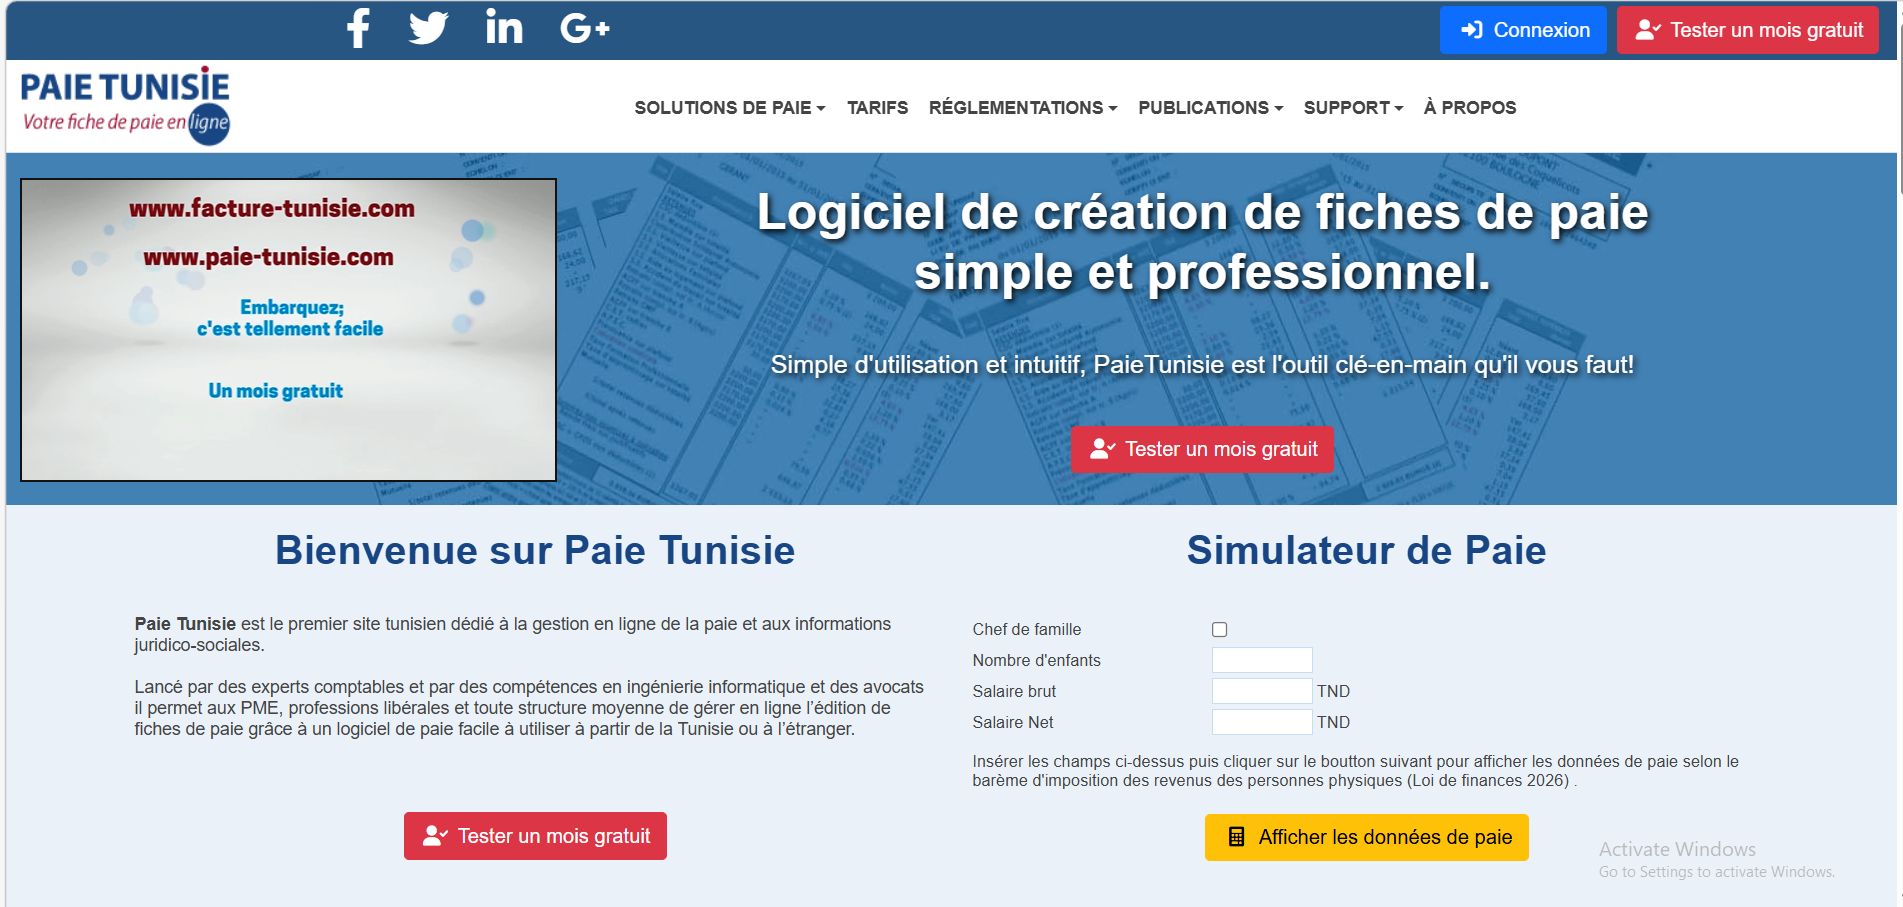
\includegraphics[width=0.9\textwidth]{paie tunisie.png}
    \caption{Paie tunisie}
\end{figure}

\subsection{Comparaison avec l'existant}
Le tableau~\ref{tab:comparaison_finale} présente une étude comparative détaillée des principales solutions de gestion RH et paie disponibles sur le marché tunisien, en les confrontant à la solution proposée PaieZone RH.

\renewcommand{\arraystretch}{2.2}
\begin{longtable}{|>{\raggedright\arraybackslash\bfseries}p{3.5cm}|>{\centering\arraybackslash}p{2.3cm}|>{\centering\arraybackslash}p{2.3cm}|>{\centering\arraybackslash}p{2.8cm}|>{\centering\arraybackslash}p{2.3cm}|}

\hline
\rowcolor[HTML]{EFEFEF}
Critères de comparaison & Excel & Logiciel Desktop & paie-tunisie.com & PaieZone RH \\ \hline
\endfirsthead

\hline
\rowcolor[HTML]{EFEFEF}
Critères de comparaison & Excel & Logiciel Desktop & paie-tunisie.com & PaieZone RH \\ \hline
\endhead

\hline
\endfoot

\caption{Étude comparative détaillée des solutions de gestion RH et paie}
\label{tab:comparaison_finale}
\endlastfoot

Accessibilité & Local uniquement & Local uniquement & Web navigateur & Web et API \\ \hline
Multi-tenant (Cabinet) & Non & Non & Non & Oui (Schéma dédié) \\ \hline
Calcul CNSS / IRPP & Manuel (formules) & Automatique & Automatique & Automatique + versionné \\ \hline
Mise à jour (Loi 2026) & Manuelle & Mise à jour éditeur & Partielle & Automatique centralisée \\ \hline
Gestion des congés & Tableau manuel & Basique & Basique & Workflow multi-niveaux \\ \hline
Pointage et Temps & Non & Partiel & Non & Complet (Badge, Import) \\ \hline
GED / Documents RH & Non & Non & Non & Oui (Archivage + Expiry) \\ \hline
Intégration comptable & Non & Partielle & Non & Auto (Plan comptable) \\ \hline
Déclarations officielles & Non & Oui & CNSS uniquement & CNSS, CAVIS, IRPP \\ \hline
Chatbot IA / RAG & Non & Non & Non & \textbf{Oui (Multi-canal)} \\ \hline
Authentification 2FA & Non & Non & Non & Oui (TOTP) \\ \hline
Journal d'audit & Non & Non & Non & Complet (Toutes actions) \\ \hline
API REST documentée & Non & Non & Non & Oui (Swagger) \\ \hline

\end{longtable}
\renewcommand{\arraystretch}{1.0}

L'analyse des solutions de gestion RH et paie disponibles sur le marché tunisien met en évidence plusieurs lacunes technologiques et fonctionnelles qui freinent l'efficacité opérationnelle des entreprises.

\begin{itemize}[label=\textbullet, leftmargin=1.5cm]
    \item \textbf{Absence d'IA et d'automatisation intelligente :}
    Aucune solution locale n'intègre actuellement d'intelligence artificielle~\cite{llm_survey}. Les interactions restent purement manuelles : l'employé doit solliciter directement le service RH pour chaque besoin (attestations, bulletins, congés). L'absence de chatbots ou d'agents conversationnels s'exprimant en langage naturel s'accompagne d'une surcharge de travail pour les gestionnaires et d'une expérience utilisateur limitée~\cite{chatbot_hr}.

    \item \textbf{Déficit de mobilité et de flexibilité (Cloud/SaaS) :}
    La prédominance des logiciels desktop restreint l'accès aux données à un poste de travail physique unique~\cite{saas}. Cette architecture interdit le travail à distance pour le comptable, la validation mobile pour le manager et la consultation en libre-service pour l'employé. De plus, le manque d'architecture multi-tenant~\cite{multitenant} empêche une gestion unifiée de plusieurs portefeuilles clients pour les cabinets d'expertise.

    \item \textbf{Lourdeur des processus administratifs :}
    La gestion des dossiers (contrats, documents administratifs, pointages) repose encore sur de nombreuses saisies répétitives. Les solutions actuelles manquent de \textit{workflows} de validation multi-niveaux automatisés (Employé $\rightarrow$ Manager $\rightarrow$ RH) et de systèmes de notifications intelligentes pour les événements critiques, tels que l'expiration des contrats CDD ou les reliquats de congés.

    \item \textbf{Complexité des mises à jour réglementaires :}
    L'évolution annuelle de la législation (notamment la \textbf{Loi de Finances 2026}~\cite{loifinance}) impose une veille constante. Sur les logiciels classiques, la mise à jour des barèmes IRPP, des taux CNSS~\cite{cnss_reg} ou du SMIG nécessite une intervention manuelle ou une réinstallation logicielle. Ce processus rigide augmente le risque d'erreurs de calcul, pouvant entraîner des bulletins non conformes et des sanctions fiscales.
\end{itemize}

\vspace{0.3cm}

\noindent Ces insuffisances justifient le besoin d'une solution moderne, centrée sur l'automatisation par l'IA et l'accessibilité SaaS~\cite{saas}, afin de répondre aux exigences de conformité et de productivité des organisations tunisiennes.

\subsection{Solution Proposée : La Plateforme PaieZone RH}\label{sec:solution}

Pour répondre aux lacunes du marché, nous proposons le développement de \textbf{PaieZone RH}, une solution SaaS multi-tenant~\cite{multitenant} nativement conçue pour moderniser la gestion sociale en Tunisie.

\subsubsection{Description et Périmètre Fonctionnel}
L'application repose sur une architecture moderne de microservices logiques. Elle centralise l'intégralité du cycle RH à travers les axes suivants :
\begingroup
\begin{itemize}[label=\textbullet, leftmargin=1.5cm]
    \item \textbf{Gestion administrative et contractuelle :} Suivi exhaustif des dossiers employés et pilotage des contrats spécifiques au droit tunisien~\cite{cdt} (CDI, CDD, CIVP, KARAMA, Stage).
    \item \textbf{Moteur de paie conforme :} Calcul automatisé intégrant les règles fiscales et sociales de la Loi de Finances 2026~\cite{loifinance} (CNSS~\cite{cnss_reg}, CAVIS, IRPP).
    \item \textbf{Pilotage des temps et activités :} Gestion dématérialisée des congés avec workflows de validation et suivi automatisé du pointage.
    \item \textbf{Déclarations et comptabilité :} Génération automatique des documents légaux et intégration fluide des écritures comptables.
    \item \textbf{Innovation IA :} Intégration d'un Chatbot RH intelligent~\cite{chatbot_hr} basé sur une architecture \textbf{RAG} (Retrieval Augmented Generation)~\cite{rag_paper}, permettant une interaction en langage naturel avec la base documentaire de l'entreprise.
\end{itemize}
\endgroup
\subsubsection{Valeur ajoutée du modèle SaaS et de l'IA}
L'adoption d'une architecture Cloud~\cite{saas} couplée à l'intelligence artificielle offre des avantages stratégiques déterminants :
\begingroup
\begin{itemize}[label=\textbullet, leftmargin=1.5cm]
    \item \textbf{Accessibilité et Mobilité :} Disponibilité universelle sur tous les terminaux, éliminant les contraintes d'installation locale et favorisant le travail collaboratif.
    \item \textbf{Efficience Multi-tenant :} Capacité pour un cabinet comptable ou une direction RH de piloter plusieurs entités (tenants)~\cite{multitenant} via une interface unique, sécurisée et isolée au niveau de la base de données.
    \item \textbf{Agilité Réglementaire :} Déploiement centralisé et instantané des mises à jour fiscales~\cite{loifinance}, garantissant une conformité permanente sans intervention manuelle des utilisateurs.
    \item \textbf{Self-service Employé par l'IA :}
    L'intégration du Chatbot RH IA~\cite{chatbot_hr} apporte une dimension innovante au self-service employé en garantissant une disponibilité continue 24h/24. Cette réactivité permet aux salariés d'obtenir un support immédiat pour leurs requêtes courantes sans solliciter directement les gestionnaires RH, optimisant ainsi le temps de chacun. Au-delà de la simple assistance, le chatbot est capable d'effectuer des automatisations directes, telles que la soumission d'une demande de congé ou la récupération instantanée d'un bulletin de paie. Enfin, grâce au système RAG~\cite{rag_paper}, l'outil fait preuve d'une véritable intelligence documentaire en interprétant de manière précise le règlement intérieur et les conventions collectives de l'entreprise pour fournir des réponses contextualisées et fiables.
    \item \textbf{Sécurité et Flexibilité :} Protection renforcée des données et modèle économique évolutif (Starter, PME, Business) adapté à la croissance de l'organisation.
\end{itemize}
\endgroup

\section{Démarche Adoptée}\label{sec:demarche}
Dans un contexte marqué par la complexité croissante des systèmes informatiques, le recours à des méthodologies de développement adaptées devient indispensable. Ces dernières visent à assurer un suivi continu du projet durant tout son cycle de vie, dans le but de produire un logiciel de haute qualité, fiable et conforme aux exigences des clients.

\subsection{Choix du cadre méthodologique}
Le développement de PaieZone RH s'inscrit dans un contexte d'incertitude partielle sur les priorités fonctionnelles et de contraintes réglementaires évolutives. Face à cette réalité, la méthodologie agile Scrum~\cite{scrum} a été choisie pour sa capacité à livrer de la valeur de manière incrémentale, à s'adapter aux changements réglementaires en cours de développement, et à impliquer régulièrement les parties prenantes dans la validation des fonctionnalités.

\subsection{Présentation de Scrum}
Scrum est un framework agile de gestion de projet~\cite{scrum} utilisé pour le développement de produits complexes et innovants. Contrairement aux méthodes traditionnelles en cascade, Scrum repose sur une approche itérative et incrémentale, ce qui permet à l'équipe de livrer progressivement des fonctionnalités tout en s'adaptant aux changements et aux retours des parties prenantes.

Le cœur de Scrum repose sur les sprints, des cycles de travail courts et réguliers au cours desquels l'équipe progresse de manière itérative pour atteindre des objectifs précis. À la fin de chaque sprint, un incrément fonctionnel du produit est livré, permettant de recueillir des retours et d'ajuster le projet si nécessaire.

\begin{figure}[htbp]
    \centering
    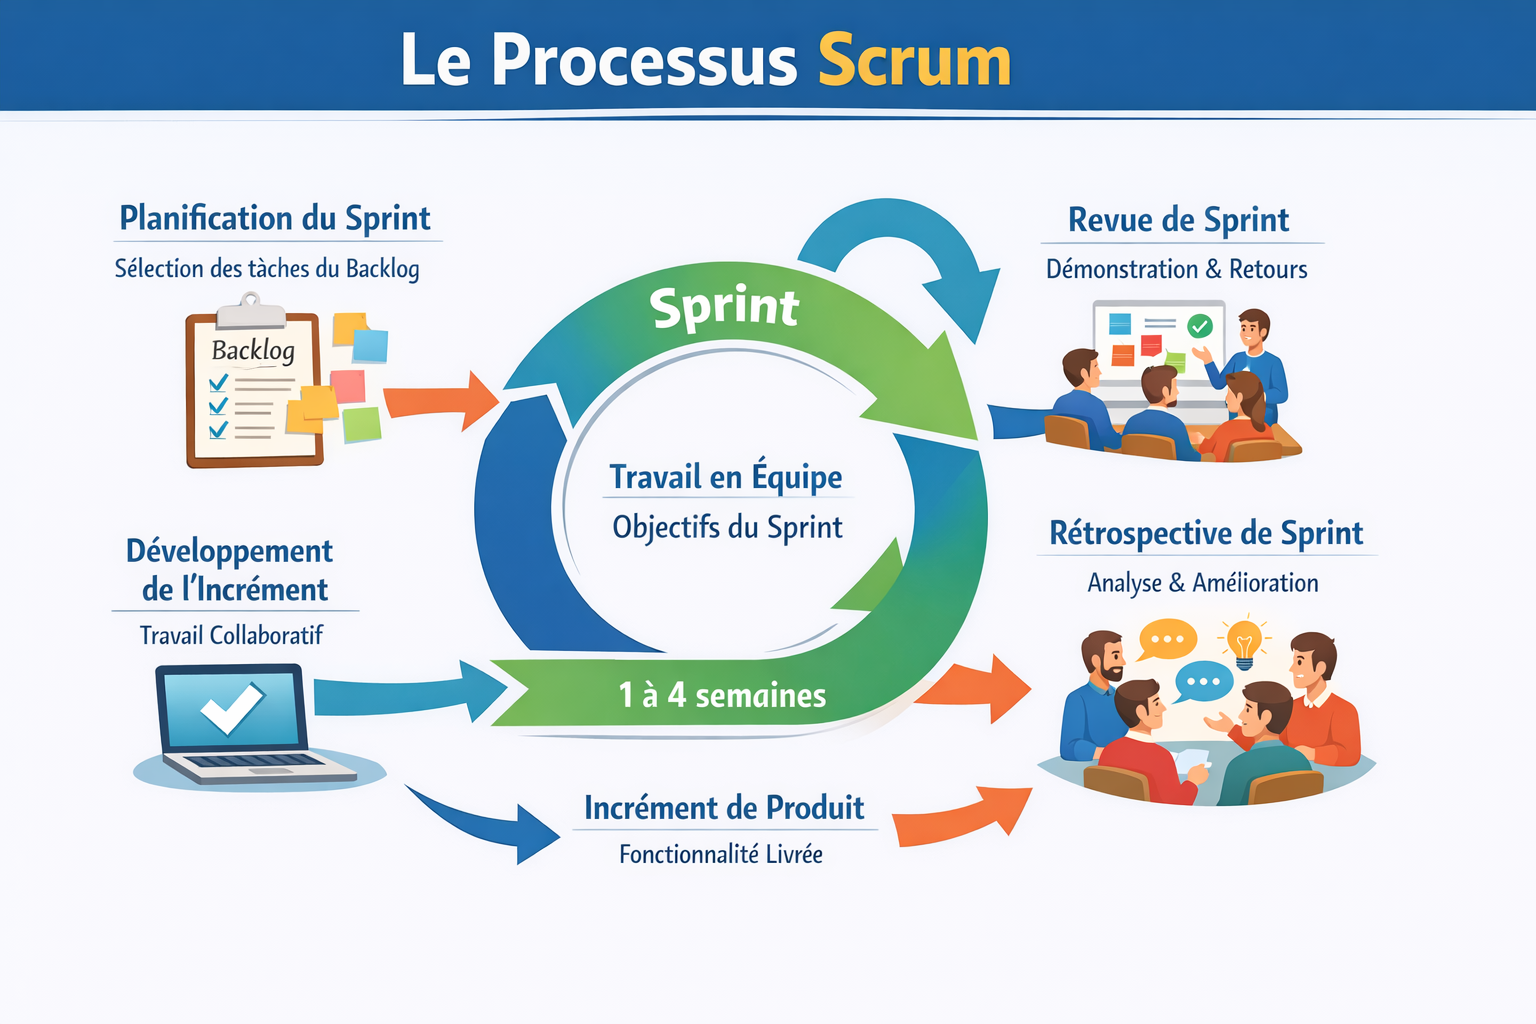
\includegraphics[width=0.9\textwidth]{scrum.png}
    \caption{Diagramme du cycle Scrum}
    \label{fig:scrum}
\end{figure}

\subsection{Raisons du choix de Scrum}
Le choix de Scrum~\cite{scrum} pour ce projet repose sur plusieurs avantages clés :
\begin{itemize}[label=\textbullet, leftmargin=1.5cm]
    \item \textbf{Livraison continue et incréments testables :} Chaque sprint produit un incrément fonctionnel et vérifiable, réduisant le risque de livrer un produit non conforme aux attentes.
    \item \textbf{Flexibilité :} Scrum permet d'intégrer facilement les changements et les nouvelles exigences tout au long du projet, sans perturber l'avancement global.
    \item \textbf{Transparence :} Les cérémonies régulières (revue, rétrospective, daily stand-up) assurent une visibilité claire sur l'état du projet et favorisent une communication fluide entre les parties prenantes.
    \item \textbf{Satisfaction client :} L'approche itérative et centrée sur la valeur métier garantit la livraison rapide de fonctionnalités utiles et adaptées aux besoins réels des clients.
    \item \textbf{Engagement de l'équipe :} Scrum encourage la collaboration, l'auto-organisation et l'amélioration continue, renforçant la motivation et l'implication des membres de l'équipe.
\end{itemize}

\subsection{Les rôles Scrum}
\begin{itemize}[label=\textbullet, leftmargin=1.5cm]
    \item \textbf{Product Owner (PO) :}
    Responsable de maximiser la valeur du produit, il gère le backlog produit, définit les priorités selon la valeur métier et communique les besoins des parties prenantes à l'équipe de développement.

    \item \textbf{Scrum Master (SM) :}
    Garant de l'application de Scrum, il facilite les cérémonies, supprime les obstacles rencontrés par l'équipe et accompagne celle-ci dans l'amélioration continue de ses pratiques.

    \item \textbf{Équipe de développement :}
    Composée de professionnels multidisciplinaires, elle est auto-organisée et responsable de la réalisation des incréments de produit à chaque sprint. L'équipe décide collectivement de la meilleure manière de transformer les éléments du backlog en fonctionnalités livrables.
\end{itemize}

\section{Langage de modélisation UML}\label{sec:uml}

Dans le cadre de la formalisation et du développement de nos idées, UML (Unified Modeling Language) constitue un langage de modélisation graphique standardisé par l'Object Management Group~\cite{uml}. Il permet de structurer, représenter et documenter un système logiciel de manière indépendante du langage de programmation utilisé. UML est également un outil de communication efficace entre les acteurs techniques et métier, offrant une représentation claire de la structure statique et du comportement dynamique des systèmes à travers différents types de diagrammes.

\begin{itemize}[label=\textbullet, leftmargin=1.5cm]
    \item \textbf{Diagramme de cas d'utilisation :}
    Le diagramme de cas d'utilisation illustre les interactions entre les acteurs et le système. Il identifie les utilisateurs (acteurs) et les fonctionnalités accessibles (cas d'utilisation). Les relations include et extend permettent de gérer les comportements communs ou optionnels. Ce diagramme constitue généralement le premier livrable dans l'analyse fonctionnelle, définissant le périmètre du système.

    \item \textbf{Diagramme de classes :}
    Le diagramme de classes représente la structure statique d'un système. Il décrit les classes, leurs attributs, leurs méthodes ainsi que les relations qui les unissent (associations, héritage, composition, agrégation). Ce diagramme sert souvent de référence pour la conception de la base de données et pour guider la génération du code.

    \item \textbf{Diagramme de séquence :}
    Le diagramme de séquence décrit la dynamique des interactions entre les composants du système dans le temps. Il montre l'ordre chronologique des messages échangés entre acteurs, objets et services pour réaliser un scénario donné. Ce diagramme est particulièrement utile pour modéliser des flux complexes incluant conditions, boucles et appels à des services externes.
\end{itemize}

\begin{figure}[htbp]
    \centering
    
\includegraphics[width=0.5\textwidth]{UML_logo.png}
    \caption{Langage de modélisation UML}
    \label{fig:uml}
\end{figure}

\section*{Conclusion}
Ce chapitre a présenté le contexte du projet, analysé les limites des solutions existantes et justifié les choix méthodologiques adoptés. Ces éléments constituent le cadre de référence sur lequel s'appuie l'ensemble du travail de conception et de développement présenté dans les chapitres suivants.

% ==========================================
% CHAPITRE 2
% ==========================================
\newpage
\chapter{Analyse et planification du projet}
\vspace{2cm}

\noindent \textbf{\Large Plan}
\vspace{1cm}
\begin{enumerate}[label=\textbf{\arabic*}, leftmargin=1.5cm, labelsep=0.8cm]
    \item[] \hspace*{-1.5cm}\textbf{Introduction} \dotfill \pageref{sec:intro_ch2}
    \item \textbf{Identification des acteurs} \dotfill \pageref{sec:acteurs}
    \item \textbf{Spécification des besoins} \dotfill \pageref{sec:besoins}
    \item \textbf{Pilotage du projet avec Scrum} \dotfill \pageref{sec:scrum_pilotage}
    \item \textbf{Backlog du Produit} \dotfill \pageref{sec:backlog}
    \item \textbf{Diagramme de cas d'utilisation global} \dotfill \pageref{sec:use_case}
    \item \textbf{Planification préliminaire des sprints} \dotfill \pageref{sec:planif_sprints}
    \item \textbf{Environnement de travail} \dotfill \pageref{sec:env_tech}
    \item \textbf{Architecture du projet} \dotfill \pageref{sec:architectures}
    \item[] \hspace*{-1.5cm}\textbf{Conclusion} \dotfill \pageref{sec:conclusion_ch2}
\end{enumerate}
\vfill
\newpage

\section*{Introduction}\label{sec:intro_ch2}
Ce chapitre constitue le pivot méthodologique entre la compréhension du contexte projet et la réalisation technique. Il couvre l'intégralité de la phase d'analyse et de planification de PaieZone RH, structurée autour de
quatre axes complémentaires.
Dans un premier temps, nous procédons à l'identification des acteurs du système et à la spécification exhaustive
des besoins fonctionnels et non fonctionnels. Dans un second temps, nous détaillons le pilotage agile du projet :
composition de l'équipe Scrum, construction du Product Backlog de 61 User Stories et planification préliminaire des
quatre sprints. Nous présentons ensuite l'environnement de travail — matériel et logiciel — ayant servi au
développement. Enfin, nous exposons les deux niveaux d'architecture retenus pour la solution : l'architecture
physique de déploiement trois-tiers et l'architecture logique N-tiers conforme aux recommandations JHipster, qui
constituent le cadre technique structurant l'ensemble du développement.
\section{Identification des acteurs}\label{sec:acteurs}
L'identification des acteurs permet de comprendre qui interagit avec le système et quelles sont leurs responsabilités respectives au sein de la solution SaaS.

Conformément au formalisme UML, une relation de généralisation lie les acteurs Admin et RH Comptable : l'acteur
Admin hérite de l'ensemble des droits et fonctionnalités de l'acteur RH Comptable, et dispose en sus de ses propres
prérogatives d'administration

Le tableau \ref{tab:acteurs} présente les différents acteurs du système ainsi que leurs responsabilités respectives.
\renewcommand{\arraystretch}{2.2}

\begin{longtable}{|>{\raggedright\arraybackslash\bfseries}p{3.5cm}|p{\dimexpr\linewidth-3.5cm-4\tabcolsep-2\arrayrulewidth}|}

\hline
\rowcolor[HTML]{EFEFEF}
\textbf{Acteur} & \textbf{Description et responsabilités} \\
\hline
\endfirsthead

\hline
\rowcolor[HTML]{EFEFEF}
\textbf{Acteur} & \textbf{Description et responsabilités} \\
\hline
\endhead
\hline
\endfoot
\hline
\caption{Tableau des acteurs et responsabilités}
\label{tab:acteurs}
\endlastfoot
Visiteur &
\begin{itemize}[label=\tiny\textbullet, nosep, leftmargin=0.4cm]
    \item Accès à la plateforme PaieZone en tant qu'internaute non authentifié.
    \item Soumission du formulaire d'inscription pour l'adhésion au service.
    \item Création simultanée du compte Administrateur et provisionnement de l'espace isolé de l'entreprise (Tenant Provisioning).
    \item Acquisition automatique du rôle Admin Entreprise à l'issue de la démarche d'inscription.
\end{itemize} \\ \hline

Utilisateur \newline (tous rôles) &
\begin{itemize}[label=\tiny\textbullet, nosep, leftmargin=0.4cm]
    \item Authentification sécurisée sur la plateforme PaieZone.
    \item Authentification à double facteur (2FA) obligatoire pour les profils Super Admin et Admin Entreprise.
\end{itemize} \\ \hline

Super Admin &
\begin{itemize}[label=\tiny\textbullet, nosep, leftmargin=0.4cm]
    \item Visualisation et supervision globale des tenants (entreprises clientes).
    \item Gestion des abonnements et des quotas de la plateforme SaaS.
    \item Maintenance globale et supervision technique du système.
    \item Configuration et mise à jour des paramètres réglementaires globaux~\cite{loifinance}.
    \item Gestion et injection automatisée par IA des matrices de conventions collectives sectorielles tunisiennes~\cite{cdt}.
\end{itemize} \\ \hline

Admin Entreprise &
\begin{itemize}[label=\tiny\textbullet, nosep, leftmargin=0.4cm]
    \item Héritage intégral des droits et fonctionnalités du profil RH Comptable.
    \item Gestion des utilisateurs internes et des rôles au sein de l'entreprise.
    \item Consultation et suivi des journaux d'audit de sécurité.
    \item Modification et mise à jour des informations légales de l'entreprise (Raison sociale, identifiant unique).
    \item Invitation de nouveaux collaborateurs sur la plateforme par email.
\end{itemize} \\ \hline

RH Comptable &
\begin{itemize}[label=\tiny\textbullet, nosep, leftmargin=0.4cm]
    \item Configuration et paramétrage de la structure organisationnelle (départements, postes).
    \item Gestion complète des dossiers salariés et des contrats de travail~\cite{cdt}.
    \item Pilotage du cycle complet de la paie et validation finale des bulletins mensuels~\cite{loifinance, cnss_reg}.
    \item Gestion opérationnelle des temps (congés, absences) et traitement des demandes d'avances.
    \item Configuration de l'intégration comptable, génération des écritures et des déclarations réglementaires.
    \item Interaction avec le chatbot IA~\cite{chatbot_hr} pour le support interne et réglementaire.
\end{itemize} \\ \hline

Employé &
\begin{itemize}[label=\tiny\textbullet, nosep, leftmargin=0.4cm]
    \item Consultation de l'espace personnel sécurisé.
    \item Visualisation, consultation et téléchargement des bulletins de paie électroniques.
    \item Soumission et suivi des demandes de congés et d'avances sur salaire.
    \item Interaction avec le chatbot IA~\cite{chatbot_hr} pour l'assistance et les requêtes RH internes.
\end{itemize} \\ 
\end{longtable}
\section{Spécification des besoins}\label{sec:besoins}

Dans cette section, nous allons nous intéresser aux besoins des utilisateurs de notre plateforme en définissant les spécifications fonctionnelles et non fonctionnelles. L'objectif est de concevoir une application performante et adaptée aux attentes du client, afin d'élaborer le Backlog du produit de manière claire et structurée.

\subsection{Besoins fonctionnels}

Les besoins fonctionnels de PaieZone ont été identifiés et organisés par acteur.

Le tableau \ref{tab:besoins-fonctionnels} présente, pour chaque acteur, l'ensemble des fonctionnalités attendues du système.

\renewcommand{\arraystretch}{1.8}

\begin{longtable}{|p{3.5cm}|p{\dimexpr\linewidth-3.5cm-4\tabcolsep-2\arrayrulewidth}|}

\hline
\rowcolor[HTML]{EFEFEF}
\textbf{Acteur} & \textbf{Fonctionnalité} \\ \hline
\endfirsthead

\hline
\rowcolor[HTML]{EFEFEF}
\textbf{Acteur} & \textbf{Fonctionnalité} \\ \hline
\endhead

\hline
\endfoot
\hline
\caption{Tableau des besoins fonctionnels par acteur}
\label{tab:besoins-fonctionnels}
\endlastfoot

% ── Utilisateur ──────────────────────────────────────────
\textbf{Utilisateur} & S'authentifier au système (2FA~\cite{totp} pour comptes sensibles) \\ \hline

% ── Super Admin ──────────────────────────────────────────
{\textbf{Super Admin}}
    & Visualiser et superviser les tenants (entreprises clientes) \\ \cline{2-2}
    & Gérer les entreprises (supprimer, suspendre, réactiver) \\ \cline{2-2}
    & Gérer les abonnements (affecter, modifier) \\ \cline{2-2}
    & Gérer les paramètres réglementaires~\cite{loifinance} (consulter, ajouter, modifier, consulter l'historique) \\ \cline{2-2}
    & Gérer les abonnements (affecter, modifier) \\ \cline{2-2}
    & Gérer le référentiel des conventions sectorielles~\cite{cdt} (consultation, modification et ajout intelligent par IA)\\ \hline

\textbf{Admin Entreprise}
    & Créer et enregistrer une entreprise \\ \cline{2-2}
    & Modifier les informations légales de l'entreprise (raison sociale, identifiant unique) \\ \cline{2-2}
    & Superviser et suivre le type d'abonnement souscrit \\ \cline{2-2}
    & Gérer les utilisateurs internes (créer, modifier, désactiver) \\ \cline{2-2}
    & Consulter et filtrer le journal d'audit \\ \cline{2-2}
    & Gérer la structure organisationnelle (départements, postes) \\ \cline{2-2}
    & Gérer les employés (créer, modifier, désactiver, consulter) \\ \cline{2-2}
    & Gérer les contrats de travail~\cite{cdt} (associer, modifier, résilier) \\ \cline{2-2}
    & Gérer les documents administratifs et légaux \\ \cline{2-2}
    & Gérer les périodes de paie (créer, modifier, clôturer) \\ \cline{2-2}
    & Gérer les rubriques et primes de paie \\ \cline{2-2}
    & Gérer les demandes d'avance (valider, refuser) \\ \cline{2-2}
    & Générer les bulletins de paie~\cite{loifinance} \\ \cline{2-2}
    & Gérer les congés et absences (types, validation, jours fériés) \\ \cline{2-2}
    & Configurer et exporter les données comptables \\ \cline{2-2}
    & Générer les déclarations réglementaires (CNSS~\cite{cnss_reg}, CAVIS, IRPP~\cite{loifinance}) \\ \cline{2-2}
    & Générer les documents officiels (attestation de salaire, certificat de travail) \\ \hline

% ── RH / Comptable ───────────────────────────────────────
\textbf{RH / Comptable}
    & Gérer la structure organisationnelle (départements, postes) \\ \cline{2-2}
    & Gérer les employés (créer, modifier, désactiver, consulter) \\ \cline{2-2}
    & Gérer les contrats de travail~\cite{cdt} (associer, modifier, résilier) \\ \cline{2-2}
    & Gérer les documents administratifs et légaux \\ \cline{2-2}
    & Consulter l'historique des modifications du dossier employé \\ \cline{2-2}
    & Gérer les périodes de paie (créer, modifier, clôturer) \\ \cline{2-2}
    & Gérer les rubriques et primes de paie \\ \cline{2-2}
    & Gérer les demandes d'avance (valider, refuser) \\ \cline{2-2}
    & Générer les bulletins de paie~\cite{loifinance} \\ \cline{2-2}
    & Gérer les congés et absences (types, validation, jours fériés) \\ \cline{2-2}
    & Configurer et exporter les données comptables \\ \cline{2-2}
    & Générer les déclarations réglementaires (CNSS salarié~\cite{cnss_reg}, CNSS employeur~\cite{cnss_reg}, CAVIS, IRPP~\cite{loifinance}) \\ \cline{2-2}
    & Générer les documents officiels (attestation de salaire, certificat de travail) \\ \hline

% ── Employé ──────────────────────────────────────────────
\textbf{Employé}
    & Consulter son espace personnel (profil, informations contractuelles) \\ \cline{2-2}
    & Visualiser et télécharger ses bulletins de paie \\ \cline{2-2}
    & Soumettre et suivre ses demandes de congés \\ \cline{2-2}
    & Consulter son solde de congés \\ \cline{2-2}
    & Soumettre une demande d'avance sur salaire \\ \cline{2-2}
    & Accéder aux services RH via le chatbot intelligent~\cite{chatbot_hr,rag_paper} (questions RH, demandes) \\ \hline

\end{longtable}

\renewcommand{\arraystretch}{1.0}

\subsection{Besoins non fonctionnels}

Au-delà des fonctionnalités métier, la qualité d'une plateforme SaaS repose sur un ensemble de contraintes non fonctionnelles qui conditionnent sa fiabilité, sa sécurité et son acceptabilité par les utilisateurs. Les exigences non fonctionnelles de PaieZone sont les suivantes :

\begin{itemize}[label=\textbullet, leftmargin=*, itemsep=6pt, topsep=6pt, parsep=0pt]
    
    \item \textbf{Sécurité et Confidentialité } La sécurité de PaieZone repose sur plusieurs mécanismes complémentaires : (i)
  l'authentification par tokens JWT à durée de vie limitée, renforcée par une authentification à deux facteurs (TOTP)
  pour les comptes à accès sensible (Super Admin, Admin) ; (ii) le contrôle d'accès basé sur les rôles (RBAC) via
  l'annotation @PreAuthorize de Spring Security, assurant que chaque utilisateur n'accède qu'aux ressources
  autorisées par son profil ; (iii) l'isolation totale des données de chaque entreprise cliente (tenant) via un
  schéma PostgreSQL dédié, rendant toute fuite inter-tenant architecturalement impossible ; (iv) un journal d'audit
  immuable (append-only) enregistrant chaque action sensible avec horodatage, identité de l'auteur, adresse IP et
  valeurs avant/après modification.

    \item \textbf{Réactivité :} L'application Angular~\cite{angular} est une Single Page Application (SPA) bénéficiant d'un design adaptatif. Les temps de réponse des API REST doivent être inférieurs à 2~secondes pour les opérations courantes. Le moteur de calcul de paie doit traiter l'intégralité des bulletins d'une société de 500 employés en moins de 30~secondes.
    
    \item \textbf{Compatibilité :} L'interface utilisateur est conçue pour fonctionner de manière optimale sur les principaux navigateurs modernes (Chrome, Firefox, Edge) et s'adapte automatiquement aux résolutions desktop et tablette, garantissant une accessibilité universelle depuis n'importe quel terminal.
    
    \item \textbf{Extensibilité :} L'architecture modulaire permet d'ajouter des modules ou des types de déclarations sans modifier l'existant. Les taux légaux sont stockés en base de données pour une mise à jour facile et modifiables via l'interface sans redéploiement applicatif, garantissant l'adaptation annuelle aux évolutions de la Loi de Finances tunisienne~\cite{loifinance}.
    
    \item \textbf{Performance :} Le système doit maintenir des temps de réponse acceptables sous charge concurrente, y compris avec
    plusieurs dizaines de tenants actifs simultanément. Le traitement des événements asynchrones (alertes d'expiration
    de contrat, notifications, messages du chatbot) ne doit pas bloquer les transactions métier synchrones. Ces
    exigences sont satisfaites grâce aux choix architecturaux détaillés à la section architecture physique.
    \item \textbf{Maintenabilité :} L'architecture modulaire de \pz\ permet l'ajout de nouveaux modules sans modification de l'existant (principe Open/Closed). Les migrations de schéma sont intégralement gérées par Liquibase de manière versionnée, garantissant la traçabilité et la reproductibilité de tout changement de base de données.
    
    \item \textbf{Portabilité :} L'ensemble des services (backend Spring Boot, base de données PostgreSQL, broker de messages) est conteneurisé via Docker, assurant un déploiement uniforme et reproductible quel que soit l'environnement cible (développement, recette, production).
    
    \item \textbf{Disponibilité :} En tant que solution SaaS, \pz\ est conçue pour une disponibilité continue. Les mises à jour réglementaires (taux CNSS, barèmes IRPP) sont déployées de manière centralisée sans interruption de service pour les tenants actifs.
\end{itemize}


\section{Pilotage du projet avec Scrum}\label{sec:scrum_pilotage}
Le pilotage de PaieZone RH s'inscrit dans le cadre méthodologique Scrum présenté au chapitre 1. Cette section
détaille la composition de l'équipe projet et l'attribution des rôles Scrum, conformément aux pratiques agiles
adoptées.

\subsection{Équipe et rôles Scrum}

Le tableau \ref{tab:equipe_scrum} suivant présente la composition de l'équipe projet et l'attribution des rôles selon le cadre Scrum~\cite{scrum} :

\begin{table}[htbp]
    \centering
    \renewcommand{\arraystretch}{1.8}
    \begin{tabularx}{\textwidth}{|>{\raggedright\arraybackslash\bfseries}p{4.2cm}|>{\raggedright\arraybackslash}p{4cm}|X|}
        \hline
        \rowcolor[HTML]{EFEFEF}
        Rôle Scrum & Membre & Fonction \\ \hline
        Product Owner  & Hadj Amor Ramzi & Directeur technique  (ComptaZone) \\ \hline
        Scrum Master & Hmidi Salim & Encadrant entreprise \newline (Grow Up Technologies) \\ \hline
        Équipe de développement & Chayma Bouguerra \newline Takwa Boughmadi & Étudiante en licence DSI \newline (ISET Mahdia) \\ \hline
    \end{tabularx}
    \caption{Équipe Scrum du projet PaieZone RH}
    \label{tab:equipe_scrum}
\end{table}
% ─────────────────────────────────────────────────────────
\section{Backlog du Produit}\label{sec:backlog}
% ─────────────────────────────────────────────────────────

Le Product Backlog est l'artefact central de la méthode Scrum~\cite{scrum}. Il constitue la liste ordonnée et priorisée de l'ensemble des fonctionnalités et améliorations attendues du produit, et représente la seule source de référence pour tout changement à y apporter. Il est la propriété exclusive du Product Owner, qui en assure la priorisation et le raffinement continu au fil du projet.

Le tableau du Product Backlog s'articule autour des colonnes suivantes, dont la définition garantit une lecture uniforme par toutes les parties prenantes :

\begin{itemize}[label=\textbullet, leftmargin=1.5cm, itemsep=0.5cm]
    \item \textbf{ID :} Identifiant unique de la User Story, permettant de la référencer sans ambiguïté dans le Product Backlog.
    \item \textbf{Épic :} Thème fonctionnel majeur regroupant plusieurs User Stories liées à un même domaine métier.
    \item \textbf{User Story :} Exigence fonctionnelle exprimée du point de vue de l'utilisateur, selon le format canonique : « En tant que [acteur], je veux [action] afin de [bénéfice métier]. »
    \item \textbf{Bénéfice métier :} Valeur attendue par l'utilisateur, exprimée sous la forme « Afin de [valeur métier] ». Les critères d'acceptation détaillés et les règles techniques sont précisés dans les backlogs de sprint correspondants (Chapitres 3 à 6).
    \item \textbf{Sprint :} Itération de développement au cours de laquelle la User Story est planifiée et réalisée. Les estimations en jours-homme associées sont détaillées dans les backlogs de sprint respectifs.
    \item \textbf{Priorité :} Niveau d'importance de la User Story pour la réussite du produit, déterminé par le Product Owner selon la valeur métier et les dépendances techniques. Quatre niveaux sont définis : Critique, Haute, Moyenne, Faible.
\end{itemize}

Le tableau~\ref{tab:backlog} présente le Product Backlog complet, organisé par épics et user stories.

\renewcommand{\arraystretch}{1.8}

\renewcommand{\arraystretch}{1.8}

\begin{xltabular}{\textwidth}{|>{\centering\arraybackslash}p{0.8cm}|>{\raggedright\arraybackslash}p{3.2cm}|>{\raggedright\arraybackslash}X|>{\raggedright\arraybackslash}X|>{\centering\arraybackslash}p{1.6cm}|}
\hline
\rowcolor[HTML]{EFEFEF}
\textbf{ID} & \textbf{Épic} & \textbf{User Story} & \textbf{Bénéfice métier} & \textbf{Priorité} \\
\hline
\endfirsthead

\hline
\rowcolor[HTML]{EFEFEF}
\textbf{ID} & \textbf{Épic} & \textbf{User Story} & \textbf{Bénéfice métier} & \textbf{Priorité} \\
\hline
\endhead

\hline
\endfoot

\caption{Product Backlog complet de PaieZone RH}
\label{tab:backlog}
\endlastfoot

% ── Épic 1 ───────────────────────────────────────────────
1 & Gestion de l'authentification et des accès
  & En tant qu'utilisateur, je veux m'authentifier~\cite{jwt}
  & Afin d'accéder au système de manière sécurisée
  & Critique \\ \hline

% ── Épic 2 ───────────────────────────────────────────────
2 & \multirow{6}{3.2cm}{Gestion des entreprises}
  & En tant qu'Admin, je veux créer une entreprise
  & Afin de l'enregistrer dans le système
  & Critique \\ \cline{3-5}
  & & En tant qu'Admin, je veux modifier une entreprise
  & Afin de mettre à jour ses informations
  & Haute \\ \cline{3-5}
  & & En tant qu'Admin, je veux désactiver une entreprise
  & Afin de suspendre son accès
  & Haute \\ \cline{3-5}
  & & En tant que Super Admin, je veux affecter un abonnement
  & Afin de gérer les droits d'accès
  & Critique \\ \cline{3-5}
  & & En tant que Super Admin, je veux modifier un abonnement
  & Afin de changer le plan souscrit
  & Moyenne \\ \cline{3-5}
  & & En tant que Super Admin, je veux résilier un abonnement
  & Afin d'arrêter le service
  & Moyenne \\ \hline

% ── Épic 3 ───────────────────────────────────────────────
3 & \multirow{3}{3.2cm}{Gestion des utilisateurs et des habilitations}
  & En tant qu'Admin, je veux créer un utilisateur
  & Afin de lui donner un accès (RBAC~\cite{rbac})
  & Critique \\ \cline{3-5}
  & & En tant qu'Admin, je veux modifier un utilisateur
  & Afin de mettre à jour ses données et ses accès
  & Haute \\ \cline{3-5}
  & & En tant qu'Admin, je veux désactiver un utilisateur
  & Afin de retirer son accès
  & Haute \\ \hline

% ── Épic 4 ───────────────────────────────────────────────
4 & \multirow{2}{3.2cm}{Traçabilité et journal d'audit}
  & En tant qu'Admin, je veux consulter le journal d'audit
  & Afin de voir les actions effectuées
  & Haute \\ \cline{3-5}
  & & En tant qu'Admin, je veux filtrer le journal d'audit
  & Afin de rechercher des actions spécifiques
  & Moyenne \\ \hline

% ── Épic 5 ───────────────────────────────────────────────
5 & \multirow{6}{3.2cm}{Gestion de la structure organisationnelle}
  & En tant qu'Admin/RH, je veux créer un département
  & Afin de structurer l'entreprise
  & Haute \\ \cline{3-5}
  & & En tant qu'Admin/RH, je veux modifier un département
  & Afin de mettre à jour la structure
  & Haute \\ \cline{3-5}
  & & En tant qu'Admin/RH, je veux désactiver un département
  & Afin de le retirer de la structure
  & Moyenne \\ \cline{3-5}
  & & En tant qu'Admin/RH, je veux créer un poste
  & Afin de définir un rôle
  & Haute \\ \cline{3-5}
  & & En tant qu'Admin/RH, je veux modifier un poste
  & Afin de l'adapter aux besoins
  & Moyenne \\ \cline{3-5}
  & & En tant qu'Admin/RH, je veux désactiver un poste
  & Afin de le retirer de la structure
  & Moyenne \\ \hline

% ── Épic 6 ───────────────────────────────────────────────
6 & \multirow{5}{3.2cm}{Gestion du capital humain}
  & En tant qu'Admin/RH, je veux consulter la liste des employés
  & Afin d'avoir une vue d'ensemble du personnel
  & Haute \\ \cline{3-5}
  & & En tant qu'Admin/RH, je veux créer un employé
  & Afin de l'ajouter au système
  & Critique \\ \cline{3-5}
  & & En tant qu'Admin/RH, je veux consulter le profil d'un employé
  & Afin de voir ses informations détaillées
  & Haute \\ \cline{3-5}
  & & En tant qu'Admin/RH, je veux modifier un employé
  & Afin de mettre à jour ses données
  & Haute \\ \cline{3-5}
  & & En tant qu'Admin/RH, je veux désactiver un employé
  & Afin de gérer sa sortie de l'organisation
  & Haute \\ \hline

% ── Épic 7 ───────────────────────────────────────────────
7 & \multirow{3}{3.2cm}{Gestion du cycle de vie des contrats de travail}
  & En tant que RH, je veux associer un contrat à un employé~\cite{cdt}
  & Afin de formaliser la relation de travail
  & Critique \\ \cline{3-5}
  & & En tant que RH, je veux modifier un contrat
  & Afin de changer ses conditions
  & Haute \\ \cline{3-5}
  & & En tant que RH, je veux résilier un contrat
  & Afin de terminer une relation de travail
  & Haute \\ \hline

% ── Épic 8 ───────────────────────────────────────────────
8 & Gestion des documents administratifs et légaux
  & En tant que RH, je veux déposer un document
  & Afin de le stocker dans le dossier employé
  & Moyenne \\ \hline

% ── Épic 9 ───────────────────────────────────────────────
9 & Historisation et suivi
  & En tant qu'Admin/RH, je veux consulter l'historique des modifications
  & Afin de tracer les changements du dossier employé
  & Haute \\ \hline

% ── Épic 10 ──────────────────────────────────────────────
10 & \multirow{4}{3.2cm}{Gestion des paramètres réglementaires}
   & En tant que Super Admin, je veux consulter la liste des paramètres réglementaires~\cite{loifinance}
   & Afin de vérifier les taux légaux en vigueur
   & Haute \\ \cline{3-5}
   & & En tant que Super Admin, je veux ajouter un nouveau paramètre réglementaire
   & Afin d'intégrer une nouvelle règle légale
   & Haute \\ \cline{3-5}
   & & En tant que Super Admin, je veux modifier un paramètre réglementaire
   & Afin de mettre à jour les taux conformément à la loi
   & Haute \\ \cline{3-5}
   & & En tant que Super Admin, je veux consulter l'historique des modifications des paramètres
   & Afin de garantir la traçabilité réglementaire
   & Moyenne \\ \hline

% ── Épic 11 ──────────────────────────────────────────────
11 & \multirow{13}{3.2cm}{Gestion de la paie}
   & En tant que RH, je veux créer une période de paie
   & Afin de lancer le cycle de traitement des salaires
   & Critique \\ \cline{3-5}
   & & En tant que RH, je veux modifier une période de paie
   & Afin de corriger les données avant clôture
   & Haute \\ \cline{3-5}
   & & En tant que RH, je veux clôturer une période de paie
   & Afin de valider et verrouiller les calculs
   & Critique \\ \cline{3-5}
   & & En tant que RH, je veux lancer le calcul de tous les bulletins d'une période
   & Afin de générer automatiquement les salaires nets~\cite{loifinance}
   & Critique \\ \cline{3-5}
   & & En tant que RH, je veux créer une rubrique de paie
   & Afin de structurer les éléments de calcul
   & Haute \\ \cline{3-5}
   & & En tant que RH, je veux modifier une rubrique de paie
   & Afin de l'adapter aux besoins de la société
   & Moyenne \\ \cline{3-5}
   & & En tant que RH, je veux ajouter une prime à un employé
   & Afin d'augmenter sa rémunération pour une période
   & Haute \\ \cline{3-5}
   & & En tant que RH, je veux modifier une prime
   & Afin d'ajuster son montant avant le calcul
   & Moyenne \\ \cline{3-5}
   & & En tant que RH, je veux valider une demande d'avance
   & Afin d'accorder le soutien financier sollicité
   & Haute \\ \cline{3-5}
   & & En tant que RH, je veux refuser une demande d'avance
   & Afin d'informer l'employé du rejet de sa demande
   & Haute \\ \cline{3-5}
   & & En tant qu'employé, je veux demander une avance sur salaire
   & Afin de recevoir un soutien financier ponctuel
   & Haute \\ \cline{3-5}
   & & En tant que RH, je veux générer un bulletin de paie
   & Afin de le distribuer à l'employé concerné
   & Critique \\ \cline{3-5}
   & & En tant que RH, je veux générer un fichier CNSS~\cite{cnss_reg}
   & Afin de déclarer les salariés auprès de la CNSS
   & Critique \\ \hline

% ── Épic 12 ──────────────────────────────────────────────
12 & \multirow{5}{3.2cm}{Gestion des congés et des absences}
   & En tant que RH, je veux créer un type de congé
   & Afin de définir les règles et quotas associés
   & Haute \\ \cline{3-5}
   & & En tant qu'employé, je veux demander un congé
   & Afin de m'absenter légitimement
   & Haute \\ \cline{3-5}
   & & En tant que RH, je veux valider une demande de congé
   & Afin de gérer la disponibilité de l'équipe
   & Haute \\ \cline{3-5}
   & & En tant qu'employé, je veux consulter mon solde de congé
   & Afin de planifier mes absences
   & Haute \\ \cline{3-5}
   & & En tant que RH, je veux gérer les jours fériés
   & Afin de les intégrer dans le calcul de paie~\cite{loifinance}
   & Moyenne \\ \hline

% ── Épic 13 ──────────────────────────────────────────────
13 & \multirow{2}{3.2cm}{Intégration comptable et finance RH}
   & En tant qu'Admin/RH, je veux configurer le plan comptable
   & Afin de structurer la comptabilité de la société
   & Haute \\ \cline{3-5}
   & & En tant qu'Admin/RH, je veux exporter les données comptables au format SAGE
   & Afin de les synchroniser avec le logiciel comptable
   & Haute \\ \hline

% ── Épic 14 ──────────────────────────────────────────────
14 & \multirow{4}{3.2cm}{Conformité et déclarations réglementaires}
   & En tant que RH, je veux générer une déclaration CNSS salarié~\cite{cnss_reg}
   & Afin de respecter les obligations légales
   & Critique \\ \cline{3-5}
   & & En tant que RH, je veux générer une déclaration CNSS employeur~\cite{cnss_reg}
   & Afin de respecter les obligations légales
   & Critique \\ \cline{3-5}
   & & En tant que RH, je veux générer une déclaration CAVIS~\cite{cnss_reg}
   & Afin de satisfaire aux obligations réglementaires
   & Haute \\ \cline{3-5}
   & & En tant que RH, je veux générer une déclaration IRPP~\cite{loifinance}
   & Afin de déclarer les retenues à la source
   & Critique \\ \hline

% ── Épic 15 ──────────────────────────────────────────────
15 & \multirow{2}{3.2cm}{Génération des documents officiels RH}
   & En tant que RH, je veux générer une attestation de salaire
   & Afin de justifier les revenus d'un employé
   & Haute \\ \cline{3-5}
   & & En tant que RH, je veux générer un certificat de travail~\cite{cdt}
   & Afin d'attester de la relation contractuelle
   & Haute \\ \hline

% ── Épic 16 ──────────────────────────────────────────────
16 & \multirow{3}{3.2cm}{Assistant RH intelligent (Chatbot)}
   & En tant qu'utilisateur, je veux accéder à un assistant conversationnel RH~\cite{chatbot_hr}
   & Afin d'obtenir des réponses rapides à mes questions administratives
   & Moyenne \\ \cline{3-5}
   & & En tant qu'employé, je veux demander un congé via le chatbot
   & Afin de simplifier la soumission de ma demande
   & Moyenne \\ \cline{3-5}
   & & En tant qu'employé, je veux consulter mon bulletin via le chatbot~\cite{rag_paper}
   & Afin d'y accéder rapidement sans navigation manuelle
   & Moyenne \\ \hline

\end{xltabular}
\renewcommand{\arraystretch}{1.0}
% ─────────────────────────────────────────────────────────
\section{Diagramme de cas d'utilisation global}\label{sec:use_case}
% ─────────────────────────────────────────────────────────
Le diagramme de cas d’utilisation global offre une synthèse structurée des interactions entre les divers acteurs et le système. Il permet d'appréhender de manière globale le périmètre fonctionnel de la solution. 

La Figure \ref{fig:use_case_global} expose ce diagramme, mettant en exergue les relations clés entre les utilisateurs et les fonctionnalités majeures de la plateforme.

\begin{figure}[h!]
    \centering
    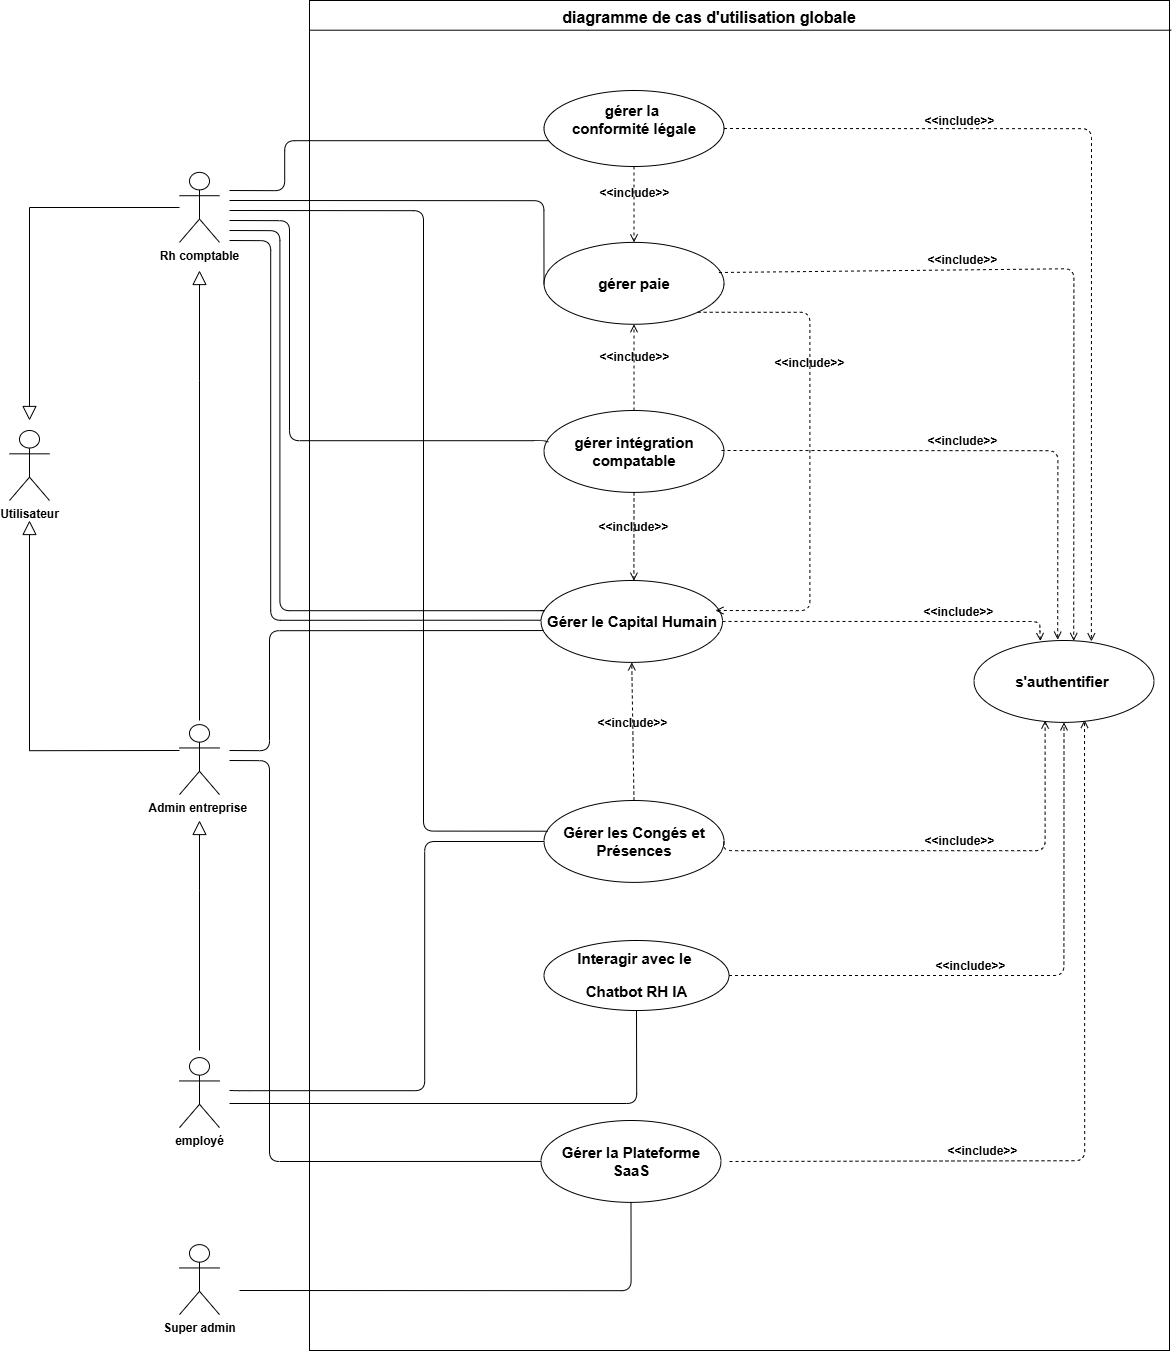
\includegraphics[width=0.9\textwidth]{diagramme-globale-F.png}
    \caption{Diagramme de cas d'utilisation global de PaieZone RH}
    \label{fig:use_case_global}
\end{figure}
\newpage

% ─────────────────────────────────────────────────────────
\section{Planification préliminaire des sprints}\label{sec:planif_sprints}
% ─────────────────────────────────────────────────────────
La planification des sprints a été établie en tenant compte de deux contraintes majeures : les dépendances techniques entre les modules et la valeur métier livrable à chaque itération. Le projet est découpé en 4 sprints de 3 semaines chacun conformément aux recommandations de Scrum~\cite{scrum}.
\newpage
\begin{table}[h]
    \centering
    \renewcommand{\arraystretch}{1.8}
    \begin{tabularx}{\textwidth}{|>{\raggedright\arraybackslash\bfseries}p{4.5cm}|X|}
        \hline
        \rowcolor[HTML]{EFEFEF}
        Sprint / Itération & Objectifs et Fonctionnalités \\ \hline
        \vspace{0.5cm}\centering
        
\includegraphics[width=2.5cm, valign=m]{sprint1.png} \par
        \textbf{Socle \& Sécurité}  &
        \begin{itemize}[label=--, nosep, leftmargin=0.4cm] \setstretch{1.6}
            \item Authentification (JWT~\cite{jwt})
            \item Inscription des entreprises
            \item Gestion des rôles et permissions (RBAC~\cite{rbac})
            \item Approbation du compte utilisateur (2FA~\cite{totp})
            \item Gestion du profil utilisateur
            \item Gestion des départements et postes
        \end{itemize} \\ \hline
        \vspace{0.1cm}\centering
        
\includegraphics[width=2.5cm, valign=m]{sprint 2.png}\par
        \textbf{Gestion Administrative} &
        \setstretch{1.6}
        \begin{itemize}[label=--, nosep, leftmargin=0.4cm]
            \item Création et suivi des dossiers employés
            \item Gestion des contrats de travail~\cite{cdt}
            \item Alertes d'expiration de contrats
            \item Historique des modifications
        \end{itemize} \\ \hline
        \vspace{0.2cm}\centering
        
\includegraphics[width=2.5cm, valign=m]{sprint 3.png}\par
        \textbf{Paie \& Congés}   &
        \begin{itemize}[label=--, nosep, leftmargin=0.4cm] \setstretch{1.6}
            \item Calcul automatique de la paie~\cite{loifinance}
            \item Gestion des congés et absences
            \item Génération des bulletins de paie
            \item Workflow de validation des congés
        \end{itemize} \\ \hline
        \vspace{0.2cm}\centering
        
\includegraphics[width=2.5cm, valign=m]{sprint 4.png} \par
        \textbf{Conformité \& IA} &
        \begin{itemize}[label=--, nosep, leftmargin=0.4cm] \setstretch{1.6}
            \item Déclarations sociales (CNSS~\cite{cnss_reg}, IRPP~\cite{loifinance})
            \item Génération des écritures comptables
            \item Chatbot RH intelligent~\cite{rag_paper,chatbot_hr}
            \item Recommandations et assistance intelligente
        \end{itemize} \\ \hline
    \end{tabularx}
    \caption{Tableau de planification préliminaire des sprints}
\end{table}
\vspace{1cm}

% ─────────────────────────────────────────────────────────
\section{Environnement de travail}\label{sec:env_tech}
% ─────────────────────────────────────────────────────────
Cette section présente l'environnement global dans lequel le projet a été conçu, développé et testé. 

Elle détaille d'une part l'infrastructure matérielle utilisée pour supporter la charge de calcul, et d'autre part l'écosystème logiciel et technique ayant servi à l'implémentation de la solution.

\subsection{Environnement matériel}
Le choix de l'architecture matérielle est une étape cruciale pour garantir la fluidité des cycles de compilation, la virtualisation des services de données et l'exécution locale des modules d'intelligence artificielle. Les ressources physiques mobilisées se répartissent sur les postes de travail décrits ci-dessous.
\subsubsection{Poste de travail n°1}
Le tableau \ref{tab:pc_chayma_final} détaille les caractéristiques techniques du premier poste de travail :

\begin{table}[htbp]
    \centering
    \renewcommand{\arraystretch}{1.5}
    \begin{tabular}{|>{\raggedright\arraybackslash\bfseries}p{5cm}|>{\raggedright\arraybackslash}p{4.9cm}|}
        \hline
        \rowcolor[HTML]{EFEFEF}
        Composant & Spécification \\ \hline
        Marque & ASUS TUF Gaming F15 \\ \hline
        Processeur & Intel Core i7-13620H \\ \hline
        Mémoire RAM & 16 Go DDR4 \\ \hline
        Disque dur & SSD NVMe 512 Go \\ \hline
        Système d'exploitation & Windows 11 Famille \\ \hline
        \multicolumn{2}{|c|}{
            \begin{minipage}{9.9cm}
                \centering
                \vspace{0.1cm}
                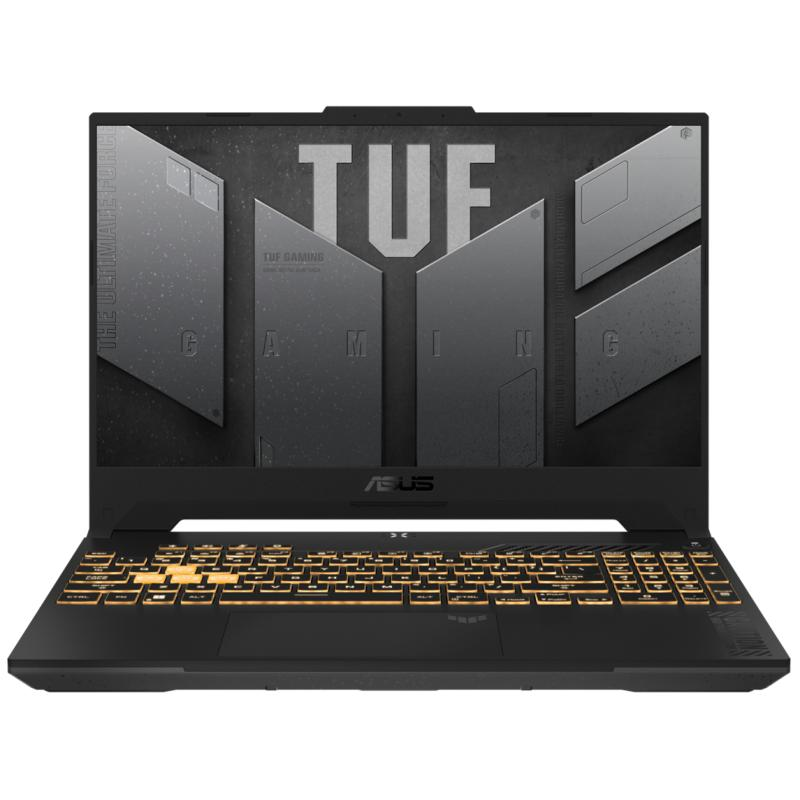
\includegraphics[height=2.5cm]{pc_chayma}
                \vspace{0.1cm}
            \end{minipage}
        } \\ \hline
    \end{tabular}
    \caption{Caractéristiques matérielles et aperçu du poste n°1}
    \label{tab:pc_chayma_final}
\end{table}

\subsubsection{Poste de travail n°2}
Le tableau \ref{tab:pc_takwa_final} détaille les caractéristiques techniques du second poste de travail :
\newpage
\begingroup
\renewcommand{\arraystretch}{1.5}
\begin{longtable}{|>{\raggedright\arraybackslash\bfseries}p{4.8cm}|>{\raggedright\arraybackslash}p{5.1cm}|}

   \hline
    \rowcolor[HTML]{EFEFEF}
    Composant & Spécification \\
    \hline
    \endfirsthead

    \endhead
    \footnotetext{}
    \endfoot
    \endfoot

    %% ── PIED DERNIÈRE PAGE ──
    \hline
    \caption{Caractéristiques matérielles et aperçu du poste n°2}
    \label{tab:pc_takwa_final}
    \endlastfoot

    Marque               & ASUS VivoBook X515EP  \\ \hline
    Processeur           & Intel Core i5-1135G7  \\ \hline
    Mémoire RAM          & 16 Go                 \\ \hline
    Disque dur           & SSD NVMe 512 Go       \\ \hline
    Système d'exploitation & Windows 11 Famille  \\ \hline

    \multicolumn{2}{|c|}{%
        \begin{minipage}{9.9cm}
            \centering
            \vspace{0.2cm}
            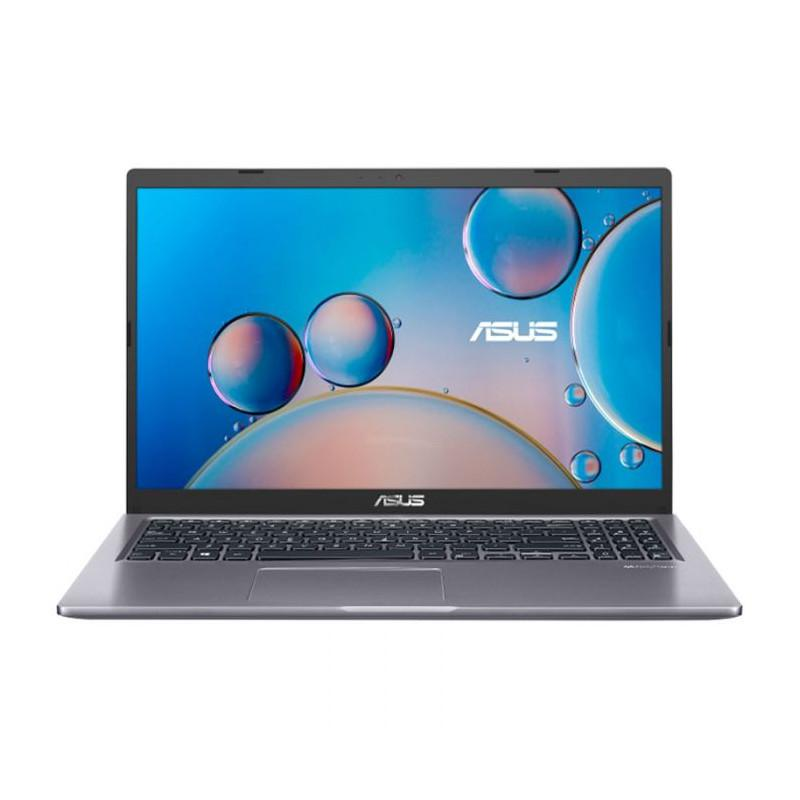
\includegraphics[height=2.5cm]{pc_takwa}
            \vspace{0.2cm}
        \end{minipage}
    } \\ \hline

\end{longtable}
\endgroup
\subsection{Environnement logiciel}

Le tableau \ref{tab:tools_logos_final} recense l'ensemble des outils et technologies utilisés pour le développement de la plateforme \pz{} :

\begingroup
\renewcommand{\arraystretch}{1.5}
% Largeur totale augmentée à 13.7 cm (parfait pour remplir l'espace de la page sans déborder)
\begin{longtable}{|>{\raggedright\arraybackslash\bfseries}p{3.2cm}|>{\raggedright\arraybackslash}p{7.5cm}|>{\centering\arraybackslash}m{3.0cm}|}
    \hline
    \rowcolor[HTML]{EFEFEF}
    Outil \& Version & Description et rôle & Logo \\
    \hline
    \endfirsthead

    \endhead
    \footnotetext{}
    \endfoot
    \endfoot

    %% ── PIED DERNIÈRE PAGE ──
    \hline
    \caption{Environnement logiciel, outils et technologies du projet}
    \label{tab:tools_logos_final}
    \endlastfoot

    JHipster 9.x~\cite{jhipster} & Générateur Full-stack utilisé pour le squelette applicatif, la sécurité JWT et les migrations Liquibase~\cite{liquibase}. & 
\includegraphics[height=1cm]{logo_jhipster} \\ \hline
    Angular 18.x~\cite{angular} & Framework frontend pour la SPA. Utilisation des \textit{signals} et de l'internationalisation FR/AR. & 
\includegraphics[height=0.9cm]{logo_angular} \\ \hline
    Spring Boot 4.0~\cite{springboot} & Backend REST sécurisé (JWT~\cite{jwt} + RBAC~\cite{rbac}). Gestion de l'audit et de l'envoi d'emails. & 
\includegraphics[height=1.2cm]{logo_springboot.png} \\ \hline
    PostgreSQL 15.x~\cite{postgresql} & Base de données relationnelle. Isolation multi-tenant~\cite{multitenant} via un schéma dédié par entreprise. & 
\includegraphics[height=1cm]{logo_postegre.png} \\ \hline
    Ollama \& Phi-3 & Environnement d'exécution de modèles de langage en local (LLM). Le modèle open-source Phi-3 (Microsoft) est exploité pour propulser le Chatbot RH intelligent, garantissant la confidentialité des données de paie sans dépendance à des API tierces payantes. & 
\includegraphics[height=1cm]{ollama.png} \\ \hline
    IntelliJ IDEA & Environnement de développement intégré (IDE) principal pour le backend Spring Boot/Java. & 
\includegraphics[height=0.9cm]{logo_intellij} \\ \hline
    GitHub & Plateforme de gestion de versions et de collaboration pour le contrôle des sources. & 
\includegraphics[height=0.9cm]{logo_github.png} \\ \hline
    Draw.io & Outil de diagrammatique en ligne utilisé pour la conception des diagrammes UML~\cite{uml} et d'architecture. & 
\includegraphics[height=0.9cm]{logo draw.png} \\ \hline
    Google Meet & Outil de visioconférence utilisé pour les réunions d'équipe et les sprints reviews. & 
\includegraphics[height=0.9cm]{google meet.png} \\ \hline
    Google Chat & Messagerie instantanée d'équipe pour les communications quotidiennes et le partage de ressources. & 
\includegraphics[height=0.9cm]{logo_intellij} \\ \hline
    Docker 24.x & Conteneurisation de tous les services pour un déploiement unifié (backend, base de données, Kafka~\cite{kafka}). & 
\includegraphics[height=1cm]{logo_docker} \\ \hline
    Lucidchart & Outil de modélisation visuelle utilisé en complément pour la conception des diagrammes de flux. & 
\includegraphics[height=0.9cm]{logo lucid.png} \\ \hline
    \LaTeX & Système de composition typographique utilisé pour la rédaction du présent rapport de PFE. & 
\includegraphics[height=0.7cm]{logo_latex.png} \\ \hline

\end{longtable}
\endgroup
% ─────────────────────────────────────────────────────────
\section{Architecture du projet}\label{sec:architectures}
% ─────────────────────────────────────────────────────────
L'architecture d'un système logiciel définit l'organisation structurelle de ses composants 
et les principes régissant leurs interactions. Pour PaieZone, deux niveaux d'architecture 
ont été définis : une architecture physique qui décrit l'organisation des composants matériels 
et réseau, et une architecture logique qui précise la structure interne du code et les couches 
applicatives.

% ── 2.8.1 ──────────────────────────────────────────────
\subsection{Architecture physique (déploiement)}
L'architecture physique de PaieZone, conforme aux principes du Cloud Computing~\cite{saas}, 
s'appuie sur un modèle trois-tiers classique, organisé en trois couches distinctes et 
indépendantes :

\begin{itemize}[label=\textbullet, leftmargin=*, itemsep=6pt, topsep=6pt, parsep=0pt]
    \item \textbf{Couche Client (Tier 1) :} Navigateurs web des utilisateurs finaux (Chrome, 
    Firefox, Edge) accédant à l'interface Angular~\cite{angular} via HTTPS. L'application est 
    une SPA : après le chargement initial, toutes les interactions avec le serveur transitent 
    par des appels API REST asynchrones (sans rechargement de page), garantissant une expérience 
    utilisateur fluide.

    \item \textbf{Couche Serveur Applicatif (Tier 2) :} Serveur hébergeant le backend Spring 
    Boot~\cite{springboot} (JAR exécutable dans un conteneur Docker). Il expose une API REST 
    documentée via Swagger/OpenAPI~3, sécurisée par tokens JWT~\cite{jwt}. Ce niveau intègre 
    également un cache applicatif assuré par Caffeine (cache en mémoire JVM) pour les données 
    fréquemment accédées (listes de tenants, paramètres réglementaires), garantissant des temps 
    de réponse optimaux sans dépendance externe, ainsi qu'Apache Kafka~\cite{kafka} comme broker 
    de messages pour le traitement asynchrone des événements non bloquants : alertes d'expiration 
    de contrats CDD, notifications de validation de congés et de demandes d'avance. Ce découplage 
    garantit la fluidité de l'application principale même sous forte charge multi-tenant.

    \item \textbf{Couche Persistance (Tier 3) :} Serveur PostgreSQL~15~\cite{postgresql}, 
    organisé en schémas multiples : un schéma public pour les données de gouvernance SaaS 
    (tenants~\cite{multitenant}, abonnements, Super Admin) et un schéma dédié 
    (ex : \texttt{tn\_acme\_sa}) pour les données métier de chaque entreprise cliente. 
    Liquibase~\cite{liquibase} assure les migrations de schéma de manière versionnée.
\end{itemize}

\begin{figure}[ht!]
    \centering
    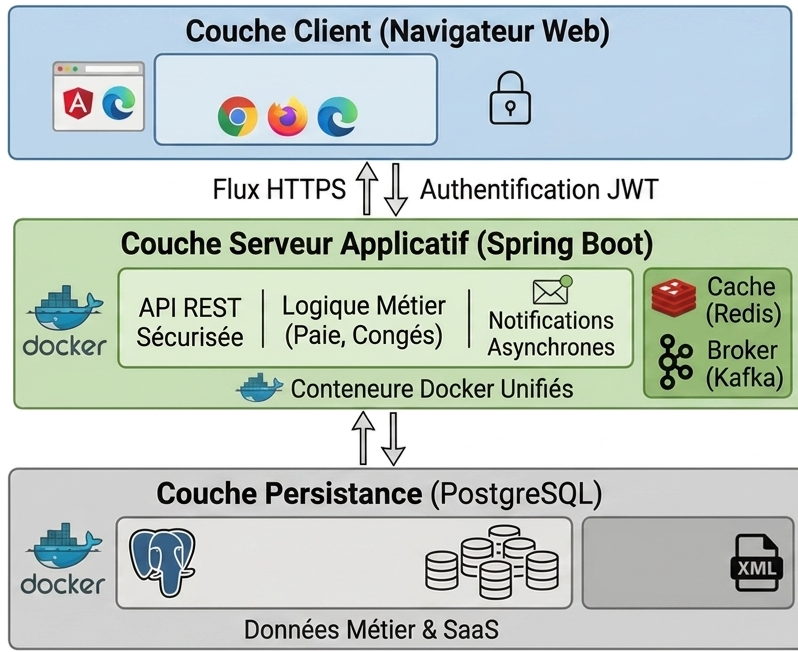
\includegraphics[width=0.87\textwidth]{architecture_logique.png}
    \caption{Architecture physique trois-tiers}
    \label{fig:architecture_physique}
\end{figure}

% ── 2.8.2 ──────────────────────────────────────────────
\subsection{Architecture logique du système}
PaieZone est développé selon une architecture N-tiers (architecture en couches), conforme 
aux recommandations JHipster~\cite{jhipster} et aux bonnes pratiques du développement Spring 
Boot~\cite{springboot}. Cette architecture s'articule autour de cinq couches verticales, 
traversées par deux couches transversales.

La figure ~\ref{fig:architecture_logique} présente les différentes couches de l'architecture 
logique du système ainsi que leurs rôles respectifs.

\begin{itemize}[label=\textbullet, leftmargin=*, itemsep=6pt, topsep=6pt, parsep=0pt]

    \item \textbf{Couche Présentation (Web Layer) :} Assurée par les contrôleurs REST Spring 
    Boot~\cite{springboot} (\texttt{@RestController}), elle expose les endpoints HTTP sous le 
    préfixe \texttt{/api/pz/}. Elle gère la validation (\texttt{@Valid}), la sérialisation 
    JSON (Jackson) et la pagination.

    \item \textbf{Couche Service (Business Layer) :} Cœur de la logique métier (annotée 
    \texttt{@Service}). Elle contient les règles de calcul de paie (Loi de Finances 
    2026~\cite{loifinance}), les workflows d'approbation et la logique 
    multi-tenant~\cite{multitenant}. La cohérence est garantie par \texttt{@Transactional}.

    \item \textbf{Couche Accès aux Données (Repository Layer) :} Implémentée via Spring Data 
    JPA et les repositories étendant \texttt{JpaRepository}. L'isolation multi-tenant est 
    assurée par un mécanisme en deux niveaux : (i) le \texttt{TenantContextService} extrait 
    l'identifiant du tenant depuis le token JWT~\cite{jwt} à chaque requête ; (ii) le 
    \texttt{DatabaseConfiguration} applique dynamiquement la commande 
    \texttt{SET search\_path TO <schema\_tenant>, public} sur la connexion 
    PostgreSQL~\cite{postgresql}, redirigeant toutes les requêtes JPA vers le schéma isolé 
    de l'entreprise concernée. Cette approche garantit qu'aucune requête ne peut accéder aux 
    données d'un autre tenant, même en cas de bug applicatif.

    \item \textbf{Couche Modèle (Domain Layer) :} Contient les entités JPA 
    (\textit{Employee, Contract, Payslip, etc.}) et les DTO assurant le découplage entre 
    persistance et présentation.

    \item \textbf{Couches transversales :} La \textbf{Sécurité} (Spring 
    Security~\cite{springboot}) valide les tokens JWT~\cite{jwt} et les rôles 
    RBAC~\cite{rbac} (\texttt{@PreAuthorize}), tandis que l'\textbf{Audit} (Spring AOP) 
    enregistre toutes les écritures dans un journal immuable.
\end{itemize}

\begin{figure}[ht!]
    \centering
    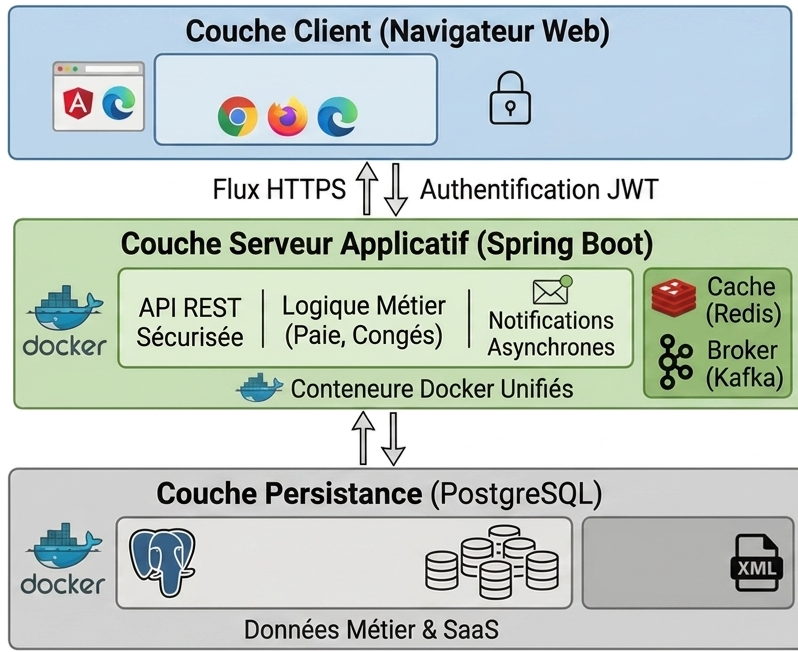
\includegraphics[width=0.85\textwidth]{architecture_logique.png}
    \caption{Architecture logique N-tiers (Spring Boot / Angular)}
    \label{fig:architecture_logique}
\end{figure}
\vfill
\newpage

% ── Conclusion ─────────────────────────────────────────
\section*{Conclusion}\label{sec:conclusion_ch2}
Ce chapitre a posé les fondements analytiques et méthodologiques du projet PaieZone RH. Nous avons défini cinq
 acteurs aux responsabilités distinctes — Visiteur, Super Admin, Admin Entreprise, RH Comptable et Employé — et
 formalisé leurs besoins à travers un Product Backlog structuré de 61 User Stories, réparties en seize épics
 fonctionnels. Les exigences non fonctionnelles identifiées — sécurité, confidentialité, performance,
 maintenabilité, portabilité et disponibilité — constituent les critères de qualité transversaux que chaque sprint
 devra respecter. L'architecture N-tiers adoptée, conforme aux recommandations JHipster, offre une séparation claire
 des responsabilités et un mécanisme multi-tenant robuste basé sur l'isolation par schéma PostgreSQL. Les choix
 technologiques retenus — Spring Boot 4.0, Angular 18, PostgreSQL 15, Kafka et Ollama — positionnent PaieZone comme
 une solution SaaS moderne, performante et évolutive. Fort de ces fondations, le chapitre suivant présente les
 travaux du premier sprint, consacré à l'implémentation du socle de sécurité, de la gestion multi-tenant et de la
 traçabilité par journal d'audit.


% ==========================================
% CHAPITRE 3
% ==========================================
\newpage
\chapter{Étude et Réalisation du Premier Sprint}
\vspace{2.5cm}

\noindent \textbf{\Large Plan}
\vspace{0.8cm}
\begin{enumerate}[label=\textbf{\arabic*}, leftmargin=1.5cm, labelsep=0.8cm]
    \item[] \hspace*{-1.5cm}\textbf{Introduction} \dotfill \pageref{sec:s1-intro}
    \item \textbf{User Stories du premier sprint} \dotfill \pageref{sec:s1-userstories}
    \item \textbf{Backlog du premier Sprint} \dotfill \pageref{sec:s1-backlog}
    \item \textbf{Spécification fonctionnelle} \dotfill \pageref{sec:s1-specification}
    \item \textbf{Conception du premier Sprint} \dotfill \pageref{sec:s1-conception}
    \item \textbf{Etude et réalisation} \dotfill \pageref{sec:s1-realisation}
    \item \textbf{Tests et Validation} \dotfill \pageref{sec:s1-tests}
    \item \textbf{Rituels Agiles } \dotfill \pageref{sec:s1-rituels}
    \item[] \hspace*{-1.5cm}\textbf{Conclusion} \dotfill \pageref{sec:s1-conclusion}
\end{enumerate}
\vfill
\newpage

\section*{Introduction}
\label{sec:s1-intro}

\addcontentsline{toc}{section}{Introduction}
Ce chapitre détaille les travaux réalisés lors du premier sprint de développement de
  PaieZone~RH. L'objectif de ce sprint était de construire le socle technique et fonctionnel
  de la plateforme, couvrant six domaines prioritaires~: le mécanisme d'authentification
  multi-rôles avec redirection contextuelle, le provisionnement automatique des espaces
  société (Tenant Provisioning), la gestion des abonnements SaaS, l'administration des
  comptes utilisateurs avec flux d'invitation par e-mail, le journal d'audit automatique par
  interception AOP, et la structuration organisationnelle (départements et postes).

  La démarche adoptée pour ce sprint suit le cycle Scrum~: planification via les User Stories,
  spécification par diagrammes de cas d'utilisation UML, conception technique par diagrammes
  de classes et de séquences, réalisation des interfaces Angular, puis validation par un plan
  de tests multiniveaux et clôture agile (Sprint Review et Rétrospective).
% ============================================================
\section{User Stories du premier sprint}
\label{sec:s1-userstories}
% ============================================================

Conformément aux méthodologies agiles, l'équipe Scrum a initié ce sprint par une réunion de planification dédiée à la formulation de l'objectif du sprint. Cet objectif, exprimé en termes métier, vise à garantir une compréhension unifiée et partagée par toutes les parties prenantes, internes comme externes à l'équipe de développement.

La question fondamentale à laquelle ce sprint répond est « Quelle valeur métier ce sprint apporte-t-il ? ». Pour ce premier incrément, l'objectif était de concrétiser les six éléments suivants du backlog, jugés prioritaires pour établir les fondations du système :

\begin{itemize}[label=\textbullet, leftmargin=0.6cm]
    \item Authentification Multi-Rôles
    \item Gestion des Entreprises
    \item Gestion des Abonnements SaaS
    \item Gestion des Utilisateurs
    \item Journal d'Audit et Traçabilité
    \item Gestion de la Structure Organisationnelle
\end{itemize}
Les besoins fonctionnels du premier sprint ont été formalisés sous forme de User Stories. 
L'intégralité de ces User Stories, incluant leurs identifiants, critères d'acceptation et 
niveaux de priorité, est détaillée dans le Tableau~\ref{tab:sprint1-us}.

\renewcommand{\arraystretch}{1.4}
\begin{small}
\begin{longtable}{|p{1.2cm}|p{9.5cm}|p{2.3cm}|}

\hline
\rowcolor[gray]{0.9}
\textbf{ID} & \textbf{User Story} & \textbf{Priorité} \\
\hline
\endfirsthead

\hline
\rowcolor[gray]{0.9}
\textbf{ID} & \textbf{User Story} & \textbf{Priorité} \\
\hline
\endhead

\hline
\endfoot
\endfoot

1.1 & En tant qu'utilisateur, je veux m'authentifier afin d'accéder au système. & Critique \\ \hline
1.2 & En tant qu'Admin, je veux m'inscrire en fournissant mes informations et celles de ma société, 
afin de créer mon espace de gestion isolé et d'en devenir le responsable. & Critique \\ \hline
2.1 & En tant qu'Admin, je veux modifier une entreprise, afin de mettre à jour ses informations 
légales. & Haute \\ \hline
2.2 & En tant qu'Admin, je veux désactiver une entreprise, afin de suspendre l'accès de l'ensemble 
de ses utilisateurs. & Haute \\ \hline
2.3 & En tant que Super Admin, je veux affecter un abonnement, afin de définir les droits et quotas 
d'une entreprise cliente. & Critique \\ \hline
2.4 & En tant que Super Admin, je veux modifier un abonnement, afin de changer le plan souscrit par 
une entreprise. & Moyenne \\ \hline
2.5 & En tant que Super Admin, je veux résilier un abonnement, afin d'arrêter le service pour une 
entreprise cliente. & Moyenne \\ \hline
3.1 & En tant qu'Admin, je veux créer un utilisateur, afin de lui donner un accès direct à la 
plateforme. & Critique \\ \hline
3.2 & En tant qu'Admin, je veux inviter un utilisateur par e-mail, afin qu'il puisse définir son 
mot de passe et activer son compte de façon sécurisée. & Haute \\ \hline
3.3 & En tant qu'Admin, je veux modifier un utilisateur, afin de mettre à jour ses données et ses 
droits d'accès. & Haute \\ \hline
3.4 & En tant qu'Admin, je veux désactiver un utilisateur, afin de retirer immédiatement son accès 
à la plateforme. & Haute \\ \hline
4.1 & En tant qu'Admin, je veux consulter le journal d'audit, afin de superviser l'ensemble des 
actions effectuées sur le système. & Haute \\ \hline
4.2 & En tant qu'Admin, je veux filtrer le journal d'audit, afin de rechercher des événements 
spécifiques par date, utilisateur ou type d'action. & Moyenne \\ \hline
5.1 & En tant qu'Admin/RH, je veux créer un département, afin de structurer la hiérarchie de 
l'entreprise. & Haute \\ \hline
5.2 & En tant qu'Admin/RH, je veux modifier un département, afin de mettre à jour ses 
informations. & Haute \\ \hline
5.3 & En tant qu'Admin/RH, je veux désactiver un département, afin de le retirer de la structure 
active. & Moyenne \\ \hline
5.4 & En tant qu'Admin/RH, je veux créer un poste, afin de définir un rôle au sein d'un 
département. & Haute \\ \hline
5.5 & En tant qu'Admin/RH, je veux modifier un poste, afin d'adapter ses attributs. & Moyenne \\ \hline
5.6 & En tant qu'Admin/RH, je veux désactiver un poste, afin de le retirer de la structure 
organisationnelle. & Moyenne \\ \hline

\caption{User Stories sélectionnées pour le premier sprint}
\label{tab:sprint1-us}
\end{longtable}
\end{small}
\renewcommand{\arraystretch}{1}
% ============================================================
\section{Backlog du premier Sprint}
\label{sec:s1-backlog}
% ============================================================

Le Backlog du produit de PaieZone, regroupant fonctionnalités et améliorations, est formalisé 
en User Stories organisées par thèmes fonctionnels. Le Tableau~\ref{tab:backlog-sprint1} détaille 
ce backlog pour le premier sprint, incluant les tâches techniques et leurs estimations en jours.
\begin{small}
\renewcommand{\arraystretch}{1.4}
\setlength{\LTleft}{\fill}
\setlength{\LTright}{\fill}
\begin{longtable}{|p{2.5cm}|p{6.0cm}|p{6.0cm}|c|}
\hline
\rowcolor[gray]{0.9} \textbf{Item} & \textbf{User Story} & \textbf{Tâches} & 
\makecell{\textbf{Est.}\\\textbf{(j)}} \\ \hline
\endfirsthead

\hline
\rowcolor[gray]{0.9} \textbf{Item} & \textbf{User Story} & \textbf{Tâches} & 
\makecell{\textbf{Est.}\\\textbf{(j)}} \\ \hline
\endhead

\hline
\endfoot
\endfoot
\endlastfoot

% ── Authentification & Inscription (2 lignes) ────────────────
\multirow{2}{*}{\centering\makecell[c]{\textbf{Authentifica-}\\ \textbf{tion \&}\\ \textbf{Inscription}}}
& \textbf{1.1} En tant qu'utilisateur, je souhaite m'authentifier à travers un login 
et un mot de passe afin d'accéder au système.
& - Créer l'interface de la page de connexion (formulaire).\newline
- Implémenter la logique d'authentification (JWT / Spring Security).\newline
- Tester l'authentification selon les différents rôles.
& \textbf{2} \\ \cline{2-4}

& \textbf{1.2} En tant qu'Admin, je souhaite m'inscrire en fournissant mes informations 
et celles de ma société afin de créer mon espace de gestion et d'en devenir le responsable.
& - Créer l'interface de la page d'inscription (formulaire).\newline
- Gérer la logique de création simultanée du compte Admin et de la Société 
(Tenant Provisioning).\newline
- Tester la procédure d'inscription complète.
& \textbf{3} \\ \hline

% ── Gestion de l'Entreprise (2 lignes) ──────────────────────
\multirow{2}{*}{\makecell[c]{\textbf{Gestion de} \\ \textbf{l'Entreprise}}}
& \textbf{2.1} En tant qu'Admin, je souhaite modifier une entreprise afin de mettre 
à jour ses informations.
& - Développer l'interface de mise à jour des données de l'entreprise.\newline
- Implémenter l'API backend pour la modification des informations de la société.\newline
- Tester la persistance des modifications en base de données.
& \textbf{1.5} \\ \cline{2-4}

& \textbf{2.2} En tant qu'Admin, je souhaite désactiver une entreprise afin de 
suspendre son accès.
& - Implémenter la logique de désactivation / blocage de l'accès au niveau backend.\newline
- Tester l'impact de la désactivation sur les accès de l'ensemble des utilisateurs 
de cette entreprise.
& \textbf{1.5} \\ \hline

% ── Gestion des Abonnements (3 lignes) ──────────────────────
\multirow{3}{*}{\centering\makecell[c]{\textbf{Gestion des}\\ \textbf{Abonnements}\\ \textbf{(SaaS)}}}
& \textbf{2.3} En tant que Super Admin, je souhaite affecter un abonnement afin de 
gérer les droits.
& - Concevoir l'interface de gestion des plans d'abonnements pour le Super Admin.\newline
- Implémenter la logique d'affectation initiale d'un plan à une entreprise.
& \textbf{1.5} \\ \cline{2-4}

& \textbf{2.4} En tant que Super Admin, je souhaite modifier un abonnement afin de 
changer le plan.
& - Ajouter les contrôles de modification de forfait sur l'interface.\newline
- Implémenter les règles de gestion des paliers et des restrictions d'accès selon 
le nouveau plan.\newline
- Tester le passage fonctionnel d'un plan à un autre (upgrade/downgrade).
& \textbf{1.5} \\ \cline{2-4}

& \textbf{2.5} En tant que Super Admin, je souhaite résilier un abonnement afin 
d'arrêter le service.
& - Développer la logique backend de coupure ou suspension des droits d'accès 
après résiliation.\newline
- Tester le blocage effectif des fonctionnalités de la plateforme.
& \textbf{1} \\ \hline

% ── Gestion des Utilisateurs (4 lignes) ─────────────────────
\multirow{4}{*}{\centering\makecell[c]{\textbf{Gestion des}\\ \textbf{Utilisateurs}}}
& \textbf{3.1} En tant qu'Admin, je souhaite créer un utilisateur afin de lui donner 
un accès direct à la plateforme.
& - Concevoir l'interface du formulaire d'ajout d'un nouvel utilisateur.\newline
- Développer l'API REST pour l'insertion de l'utilisateur lié à la société.
& \textbf{1.5} \\ \cline{2-4}

& \textbf{3.2} En tant qu'Admin, je souhaite inviter un utilisateur par e-mail afin 
qu'il puisse définir son mot de passe lors de sa première connexion.
& - Implémenter le service de génération de token d'invitation (validité~: 7 jours).\newline
- Développer l'API REST \texttt{/api/invitations/accept}.\newline
- Tester le flux complet~: envoi email $\rightarrow$ activation du compte 
$\rightarrow$ définition du mot de passe.
& \textbf{2} \\ \cline{2-4}

& \textbf{3.3} En tant qu'Admin, je souhaite modifier un utilisateur afin de mettre 
à jour ses données et ses accès.
& - Concevoir l'interface de modification et la table de consultation des utilisateurs.\newline
- Développer l'API REST pour la mise à jour des profils.\newline
- Tester l'attribution et la modification des rôles.
& \textbf{1.5} \\ \cline{2-4}

& \textbf{3.4} En tant qu'Admin, je souhaite désactiver un utilisateur afin de 
retirer immédiatement son accès à la plateforme.
& - Implémenter la logique backend de désactivation du compte utilisateur.\newline
- Tester le refus d'accès pour un utilisateur désactivé.
& \textbf{1} \\ \hline

% ── Journal d'Audit (2 lignes) ───────────────────────────────
\multirow{2}{*}{\centering\makecell[c]{\textbf{Journal}\\ \textbf{d'Audit}}}
& \textbf{4.1} En tant qu'Admin, je souhaite consulter le journal d'audit afin de 
voir les actions effectuées.
& - Créer le composant d'affichage de l'historique des actions (tableau UI).\newline
- Implémenter le système d'interception et d'enregistrement automatique des 
actions (AOP / Spring).
& \textbf{1.5} \\ \cline{2-4}

& \textbf{4.2} En tant qu'Admin, je souhaite filtrer le journal d'audit afin de 
rechercher des actions spécifiques.
& - Mettre en place les composants graphiques des filtres (par date, par utilisateur, 
par action).\newline
- Développer la logique de filtrage des requêtes côté backend.
& \textbf{1.5} \\ \hline

% ── Gestion Organisationnelle (6 lignes) ─────────────────────
\multirow{4}{*}{\centering\makecell[c]{\textbf{Gestion des}\\ \textbf{Utilisateurs}}}
& \textbf{5.1} En tant qu'Admin/RH, je souhaite créer un département afin de 
structurer l'entreprise.
& - Concevoir l'interface de création d'un département.\newline
- Développer le service backend d'insertion avec les validations nécessaires.
& \textbf{1} \\ \cline{2-4}

& \textbf{5.2} En tant qu'Admin/RH, je souhaite modifier un département afin de 
mettre à jour la structure.
& - Créer l'interface de modification des informations d'un département.\newline
- Mettre à jour le service backend correspondant.
& \textbf{1} \\ \cline{2-4}

& \textbf{5.3} En tant qu'Admin/RH, je souhaite désactiver un département afin de 
le retirer de la structure.
& - Implémenter la logique de désactivation logique d'un département.\newline
- Tester la désactivation d'un département contenant encore des postes actifs.
& \textbf{1} \\ \cline{2-4}

& \textbf{5.4} En tant qu'Admin/RH, je souhaite créer un poste afin de définir 
un rôle au sein d'un département.
& - Concevoir l'interface de création d'un poste (rattaché à un département).\newline
- Développer le service d'insertion backend pour les postes.
& \textbf{1} \\ \cline{2-4}

& \textbf{5.5} En tant qu'Admin/RH, je souhaite modifier un poste afin d'adapter 
ses attributs.
& - Créer l'interface de modification des données d'un poste.\newline
- Implémenter la mise à jour des données en base.
& \textbf{1} \\ \cline{2-4}

& \textbf{5.6} En tant qu'Admin/RH, je souhaite désactiver un poste afin de le 
retirer de la structure organisationnelle.
& - Implémenter la logique backend de retrait/désactivation d'un poste.\newline
- Tester la cohérence de l'organigramme suite à cette suppression.
& \textbf{1} \\ \hline

\caption{Backlog détaillé du premier Sprint}
\label{tab:backlog-sprint1}
\end{longtable}
\end{small}
\renewcommand{\arraystretch}{1.0}
\normalsize
% ============================================================
\section{Spécification fonctionnelle du premier Sprint}
\label{sec:s1-specification}
% ============================================================
La modélisation fonctionnelle de PaieZone a été réalisée via des diagrammes de cas 
d'utilisation UML, offrant une vue globale des fonctionnalités du Sprint~1, complétés 
par des descriptions textuelles détaillant les scénarios d'interaction. Cette approche 
permet de représenter visuellement le périmètre du système et les interactions clés.

% -----------------------------------------------------------
\subsection{Diagramme de cas d'utilisation du premier Sprint}
% -----------------------------------------------------------
La figure~\ref{fig:use-case-s1} présente le diagramme de cas d'utilisation raffiné 
du Sprint~1 de PaieZone~RH, structuré autour de cinq acteurs et de six packages 
fonctionnels.

\begin{figure}[htbp]
    \centering
    \vspace*{-0.18cm}
    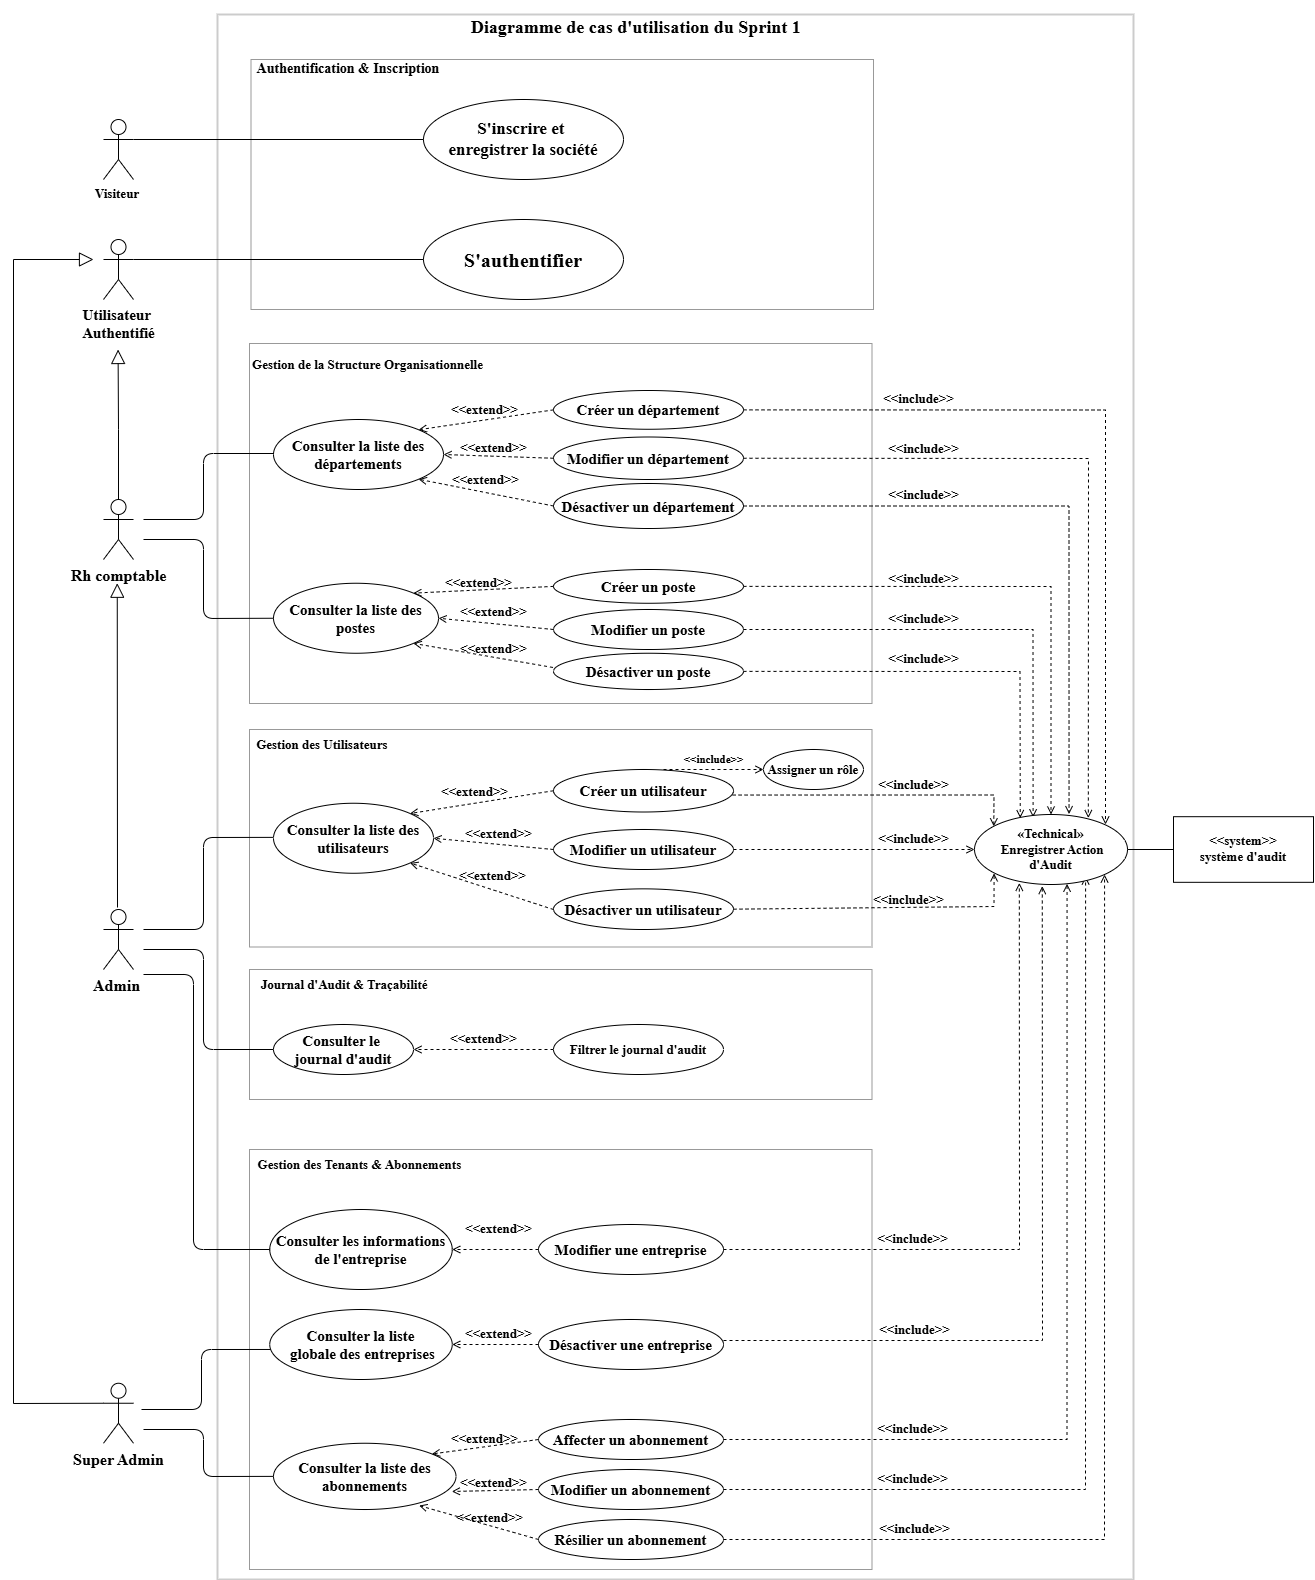
\includegraphics[width=0.95\textwidth]{use-case-sp1}
    \caption{Diagramme de cas d'utilisation raffiné du Sprint~1}
    \label{fig:use-case-s1}
\end{figure}

Le diagramme s'organise comme suit :

\medskip
\noindent\textbf{Relations structurelles UML :}
Le cas d'utilisation \og{}S'authentifier\fg{} est en relation \texttt{<<include>>} 
avec l'ensemble des cas d'utilisation protégés, matérialisant la précondition d'accès 
obligatoire. La vérification 2FA étend (\texttt{<<extend>>}) le flux nominal 
d'authentification pour les comptes Super Admin et Admin. Une relation de 
généralisation unit les acteurs \textsc{Admin} et \textsc{RH}~: l'Admin hérite de 
tous les cas d'utilisation du RH et dispose en sus de ses propres prérogatives.
\medskip
\noindent\textbf{Responsabilités par acteur :}

\begin{itemize}[label=\textbullet, leftmargin=0.6cm]

  \item \textbf{Visiteur :} Unique acteur non authentifié. Déclenche le cas 
  d'utilisation \og{}S'inscrire et enregistrer la société\fg{}, qui initie 
  automatiquement le Tenant Provisioning (création du schéma PostgreSQL dédié). 
  À l'issue de ce flux, le Visiteur acquiert le rôle Admin Entreprise.

  \item \textbf{Utilisateur (rôle générique) :} Regroupe tout compte authentifié, 
  quel que soit son rôle. Il peut s'authentifier, activer la 2FA et gérer son profil.

  \item \textbf{Admin Entreprise :} Gère les informations légales de la société, 
  administre les comptes utilisateurs (création directe ou invitation par e-mail), 
  configure la structure organisationnelle et consulte le journal d'audit.

  \item \textbf{Super Admin :} Supervise les entreprises clientes et pilote les 
  abonnements SaaS (affectation, modification, résiliation).

  \item \textbf{RH Comptable :} Dans le périmètre du Sprint~1, intervient 
  uniquement dans la définition de la structure organisationnelle (départements 
  et postes).

\end{itemize}

% -----------------------------------------------------------
\subsection{Description textuelle des cas d'utilisation}
% -----------------------------------------------------------
Les descriptions textuelles détaillent les préconditions et scénarios (nominaux et 
alternatifs) des cas d'utilisation. Elles servent de référence contractuelle pour 
valider les fonctionnalités du sprint avec le Product Owner.

% -----------------------------------------------------------
\subsubsection{Cas d'utilisation 1 : S'authentifier}
% -----------------------------------------------------------
Le tableau~\ref{tab:uc_authentification} présente la description textuelle détaillée 
du cas d'utilisation \og{}S'authentifier\fg{}.

\vspace{0.2cm}
\begin{xltabular}{\textwidth}{|l|X|}
    \hline
    \rowcolor[gray]{0.9} \textbf{Élément} & \textbf{Description} \\ \hline
    \endfirsthead
    \hline
    \rowcolor[gray]{0.9} \textbf{Élément} & \textbf{Description} \\ \hline
    \endhead
    \hline
    \endfoot
    \endfoot
    \endlastfoot
    \textbf{Titre} & S'authentifier \\ \hline
    \textbf{Acteur principal} & Utilisateur (Admin, RH Comptable, Super Admin, Employé) \\ \hline
    \textbf{Préconditions} & L'utilisateur dispose d'un compte actif, non suspendu, 
    et de ses identifiants de connexion (e-mail et mot de passe). \\ \hline
    \textbf{Postconditions} & Un token JWT est généré et transmis au client. 
    L'utilisateur est redirigé vers le tableau de bord correspondant à son rôle. \\ \hline
    \textbf{Scénario principal} &
    \begin{enumerate}[nosep, leftmargin=*]
        \item L'utilisateur accède à l'interface de connexion.
        \item Il saisit son adresse e-mail et son mot de passe.
        \item Le système vérifie les identifiants et contrôle le statut du compte 
              (actif / suspendu).
        \item Un token JWT signé (durée de vie limitée) est généré et retourné 
              au client Angular.
        \item Le système identifie le rôle et le tenant de l'utilisateur depuis 
              le payload du token.
        \item L'utilisateur est redirigé vers le tableau de bord correspondant 
              à son rôle (\texttt{ROLE\_SUPER\_ADMIN}, \texttt{ROLE\_ADMIN}, 
              \texttt{ROLE\_RH\_COMPTABLE} ou \texttt{ROLE\_EMPLOYE}).
    \end{enumerate} \\ \hline
    \textbf{Scénarios alternatifs}
    & \textbf{A1 : Identifiants incorrects} $\rightarrow$ Le système affiche un 
      message d'erreur générique et invite à une nouvelle saisie (sans préciser 
      si c'est l'e-mail ou le mot de passe qui est erroné, pour éviter 
      l'énumération de comptes). \\ \cline{2-2}
    & \textbf{A2 : Compte suspendu} $\rightarrow$ Le système informe l'utilisateur 
      que son accès a été désactivé et l'invite à contacter l'administrateur. \\ \cline{2-2}
    & \textbf{A3 : Authentification 2FA requise} $\rightarrow$ Pour les comptes 
      Super Admin et Admin, après validation du mot de passe, le système exige 
      la saisie d'un code TOTP (Time-based One-Time Password) généré par 
      l'application d'authentification de l'utilisateur. \\ \hline
      \caption{Description textuelle du cas d'utilisation S'authentifier}
    \label{tab:uc_authentification}
\end{xltabular}

% -----------------------------------------------------------
\subsubsection{Cas d'utilisation 2 : S'inscrire et enregistrer la société}
% -----------------------------------------------------------
Le tableau~\ref{tab:uc_inscription} présente la description textuelle détaillée du 
cas d'utilisation \og{}S'inscrire et enregistrer la société\fg{}.

\vspace{0.2cm}
\begin{xltabular}{\textwidth}{|l|X|}
    
    \hline
    \rowcolor[gray]{0.9} \textbf{Élément} & \textbf{Description} \\ \hline
    \endfirsthead
    \hline
    \rowcolor[gray]{0.9} \textbf{Élément} & \textbf{Description} \\ \hline
    \endhead
    \hline
    \endfoot
    \endfoot
    \endlastfoot

    \textbf{Titre} & S'inscrire et enregistrer la société \\ \hline
    \textbf{Acteur principal} & Visiteur \\ \hline
    \textbf{Préconditions} & Le visiteur ne possède pas de compte PaieZone. 
    L'adresse e-mail et le matricule fiscal de la société renseignés ne sont 
    pas déjà enregistrés dans le système. \\ \hline
    \textbf{Postconditions} & Un schéma PostgreSQL isolé est créé pour la société 
    (Tenant Provisioning). Les migrations Liquibase sont appliquées automatiquement. 
    Le visiteur devient l'Administrateur responsable de cet espace et son compte 
    est activé. Un e-mail de confirmation est envoyé. \\ \hline
    \textbf{Scénario principal} &
    \begin{enumerate}[nosep, leftmargin=*]
        \item Le visiteur accède au formulaire d'inscription.
        \item Il renseigne ses informations personnelles (nom, prénom, e-mail, 
              mot de passe) et les informations légales de sa société 
              (raison sociale, matricule fiscal, adresse).
        \item Le système valide les données transmises (format, unicité).
        \item Un schéma PostgreSQL dédié est créé pour la société et les migrations 
              Liquibase sont appliquées, initialisant la structure de la base de 
              données du tenant.
        \item Un compte Administrateur est créé et associé à la société.
        \item Un e-mail de confirmation d'inscription est envoyé à l'adresse fournie.
        \item Le visiteur (désormais Administrateur) est redirigé vers la page 
              de connexion.
    \end{enumerate} \\ \hline
    \textbf{Scénarios alternatifs}
    & \textbf{A1 : Adresse e-mail déjà utilisée} $\rightarrow$ Le système affiche 
      un message d'erreur indiquant que l'e-mail est déjà associé à un compte 
      existant. \\ \cline{2-2}
    & \textbf{A2 : Données invalides} $\rightarrow$ Le système affiche les erreurs 
      de validation spécifiques sur les champs concernés. \\ \cline{2-2}
    & \textbf{A3 : Matricule fiscal déjà enregistré} $\rightarrow$ Le système 
      bloque la création et indique que cette société est déjà inscrite sur 
      la plateforme. 
      \\ \hline
    \caption{Description textuelle du cas d'utilisation S'inscrire et enregistrer la société}
    \label{tab:uc_inscription}
\end{xltabular}

% -----------------------------------------------------------
\subsubsection{Cas d'utilisation 3 : Gérer les utilisateurs}
% -----------------------------------------------------------
Le tableau~\ref{tab:uc_gestion_utilisateurs} présente la description textuelle 
détaillée du cas d'utilisation \og{}Gérer les utilisateurs\fg{}.

\vspace{0.2cm}
\begin{xltabular}{\textwidth}{|l|X|}
    
    \hline
    \rowcolor[gray]{0.9} \textbf{Élément} & \textbf{Description} \\ \hline
    \endfirsthead
    \hline
    \rowcolor[gray]{0.9} \textbf{Élément} & \textbf{Description} \\ \hline
    \endhead
    \hline
    \endfoot
    \endfoot
    \endlastfoot

    \textbf{Titre} & Gérer les utilisateurs (Créer / Inviter / Modifier / 
    Désactiver) \\ \hline
    \textbf{Acteur principal} & Admin \\ \hline
    \textbf{Préconditions} & L'Administrateur est authentifié et dispose des droits 
    de gestion des utilisateurs sur son tenant. \\ \hline
    \textbf{Postconditions} & L'utilisateur ciblé est créé, invité, modifié ou 
    désactivé. L'action est enregistrée automatiquement dans le journal d'audit 
    (interception AOP). \\ \hline
    \textbf{Scénario principal} &
    \begin{enumerate}[nosep, leftmargin=*]
        \item L'Administrateur accède à l'interface de gestion des utilisateurs.
        \item Il consulte la liste paginée des utilisateurs de sa société.
        \item Il sélectionne l'action souhaitée :
        \begin{itemize}[nosep, leftmargin=*]
            \item \textbf{Création directe :} renseigne les informations 
                  (nom, e-mail, rôle) et confirme ; un compte activé est créé.
            \item \textbf{Invitation par e-mail :} saisit l'e-mail et le rôle ; 
                  le système génère un token d'invitation (validité 7~jours) et 
                  envoie un lien d'activation ; le compte reste inactif jusqu'à 
                  l'acceptation.
            \item \textbf{Modification :} met à jour les informations ou le rôle 
                  d'un compte existant.
            \item \textbf{Désactivation :} révoque immédiatement les droits d'accès.
        \end{itemize}
        \item Le système valide les données et applique les changements en base 
              de données ; l'action est tracée automatiquement dans le journal 
              d'audit (horodatage, identité de l'auteur, valeurs avant/après).
        \item Un message de confirmation est affiché.
    \end{enumerate} \\ \hline
    \textbf{Scénarios alternatifs}
    & \textbf{A1 : Utilisateur introuvable} $\rightarrow$ Le système affiche 
      un message d'erreur. \\ \cline{2-2}
    & \textbf{A2 : Droits insuffisants} $\rightarrow$ Exception 403 levée 
      par Spring Security. \\ \cline{2-2}
    & \textbf{A3 : E-mail déjà utilisé} $\rightarrow$ Le système bloque 
      l'enregistrement. \\ \cline{2-2}
    & \textbf{A4 : Token d'invitation expiré} $\rightarrow$ Le système invalide 
      le lien et invite l'utilisateur à contacter l'administrateur pour 
      un renvoi.
    \\ \hline
    \caption{Description textuelle du cas d'utilisation Gérer les utilisateurs}
    \label{tab:uc_gestion_utilisateurs} 
\end{xltabular}
% ============================================================
\section{Conception du premier Sprint}
\label{sec:s1-conception}
% ============================================================
La conception technique de PaieZone~RH matérialise les besoins métiers à travers des 
modèles structurants guidant le développement. Cette section s'articule autour de deux 
axes complémentaires~: le diagramme de classes, qui décrit l'architecture statique des 
entités, et les diagrammes de séquences, qui modélisent la dynamique des interactions.

% ============================================================
\subsection{Diagramme de classes}
% ============================================================
Le diagramme de classes modélise l'architecture statique du système. Il définit la 
structure des données en précisant les entités, leurs attributs et les relations de 
dépendance qui les unissent, offrant ainsi une vue d'ensemble de l'organisation logique 
de PaieZone.

\begin{figure}[htbp]
    \centering
    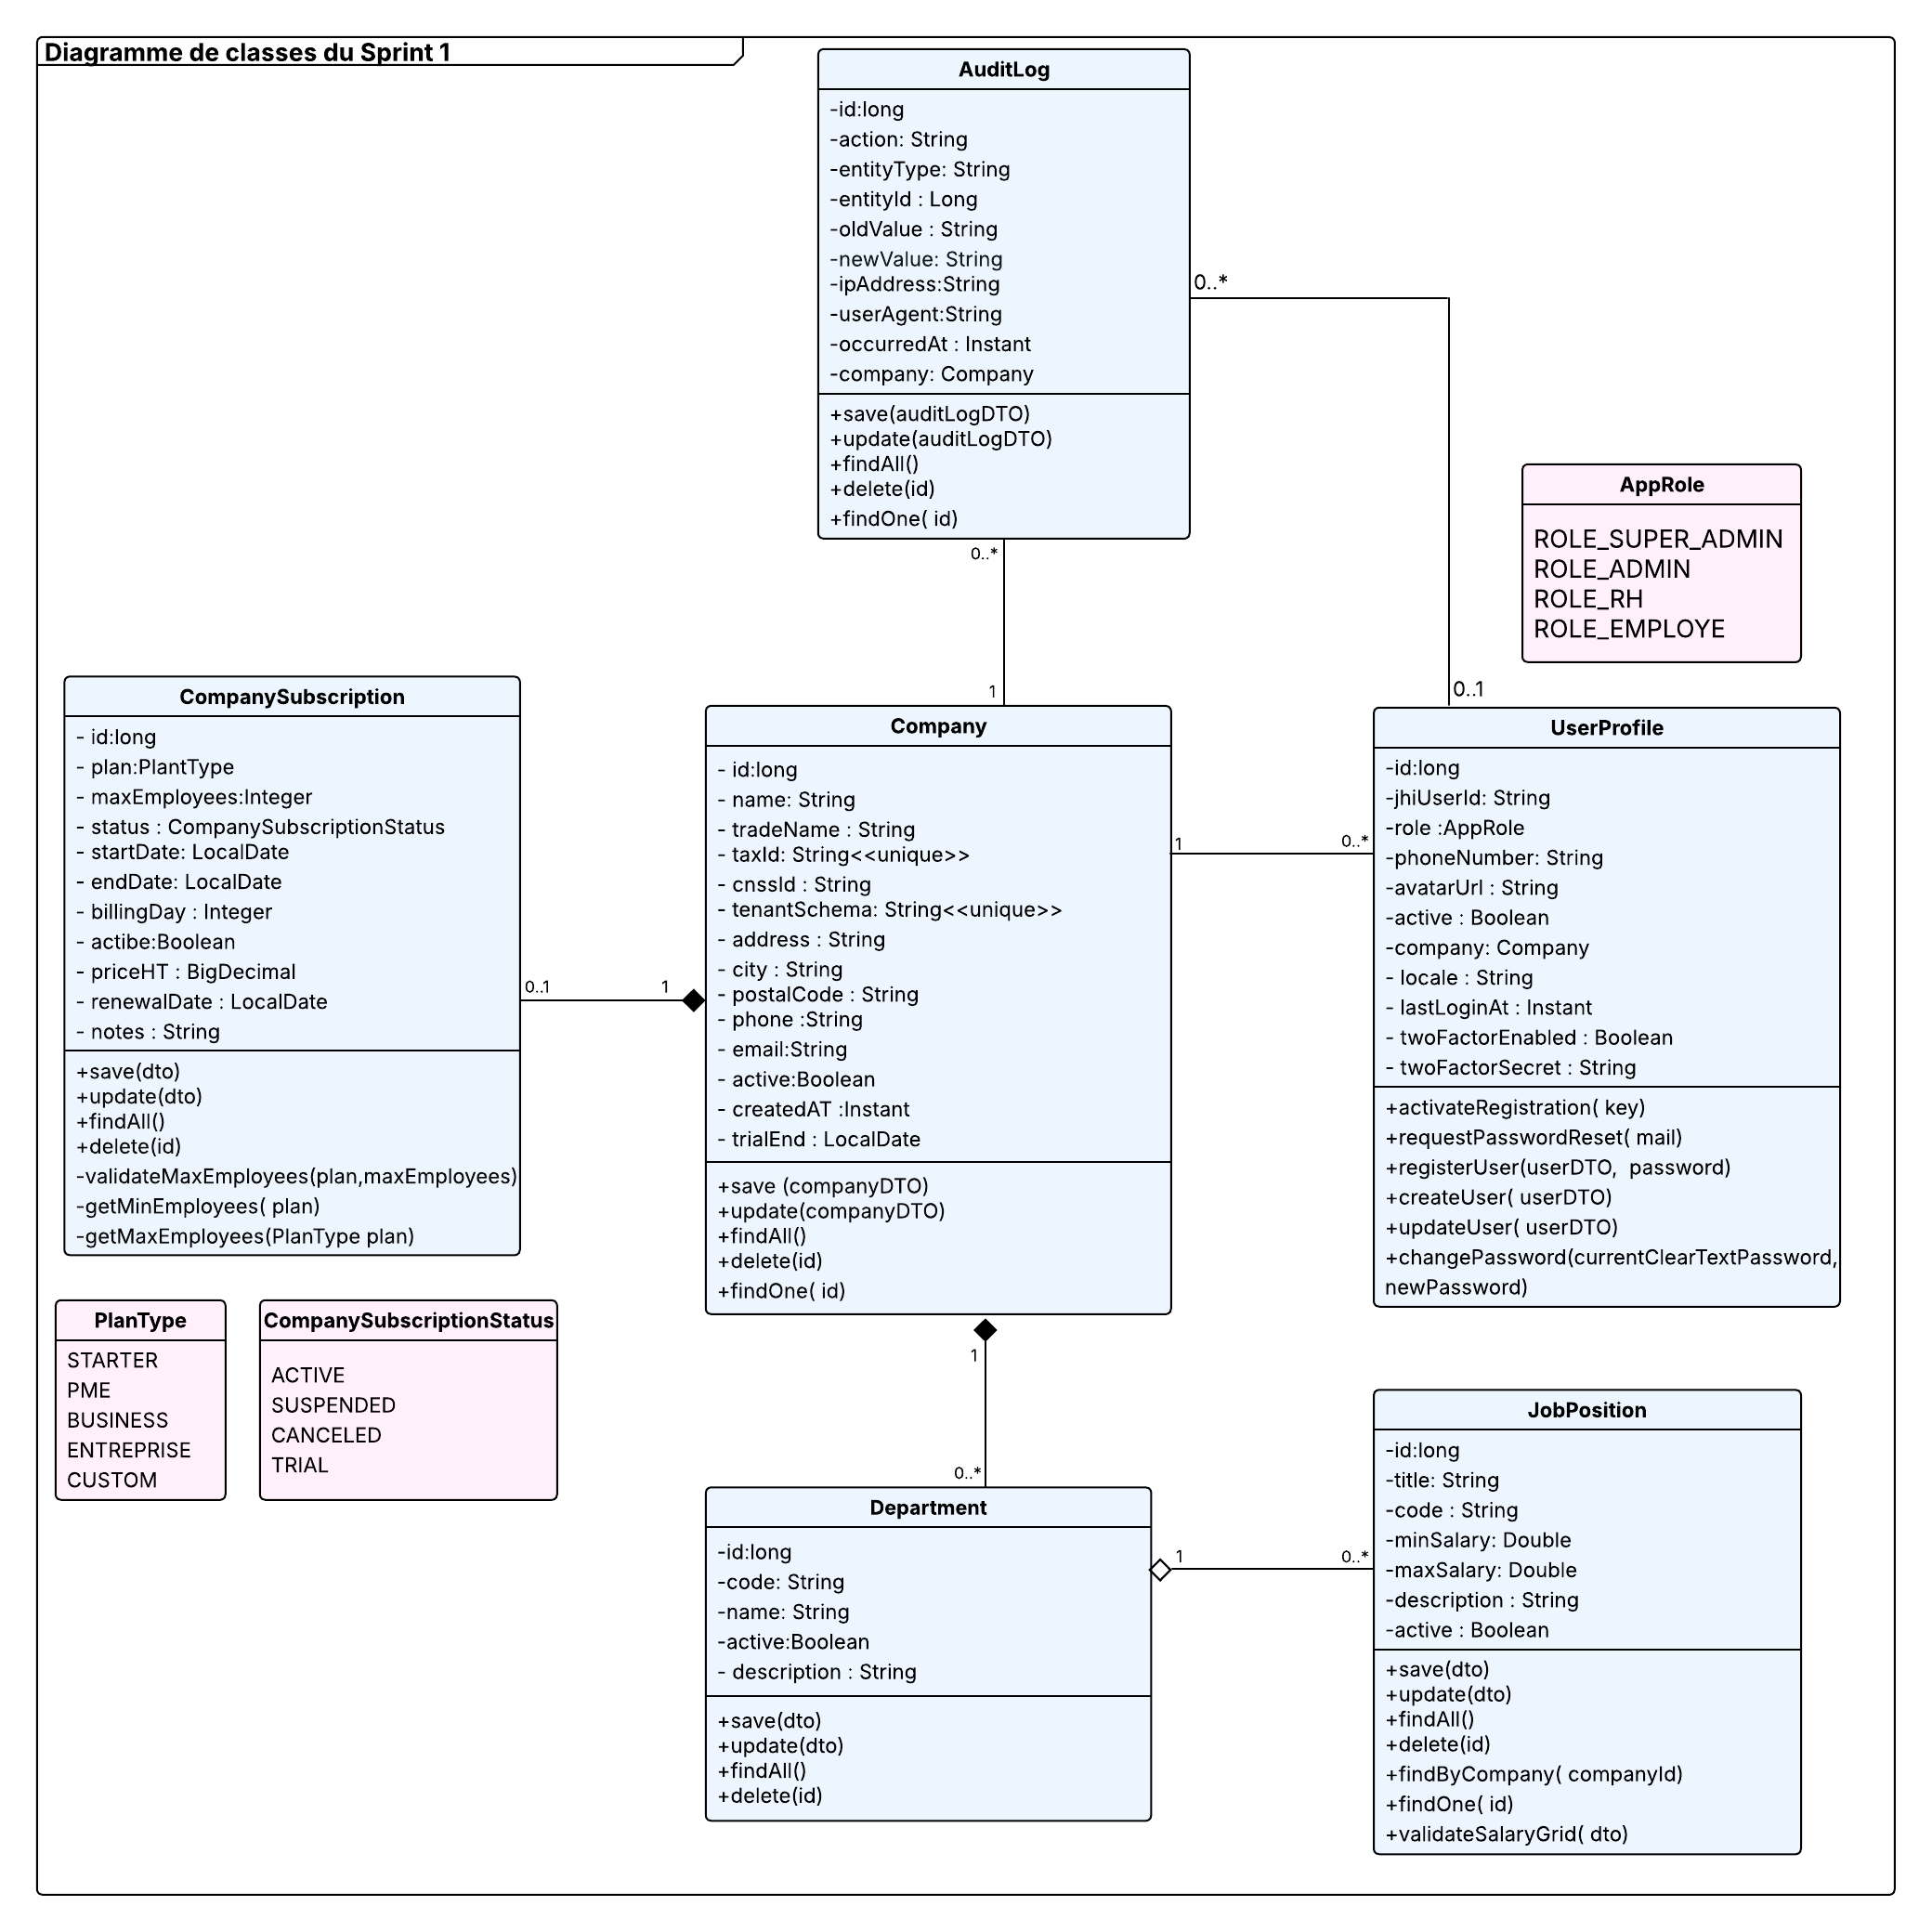
\includegraphics[width=0.99\textwidth]{classes-sprint1}
    \caption{Diagramme de classes du Sprint~1}
    \label{fig:classes-sprint1}
\end{figure}
La structure statique des données pour ce premier sprint est modélisée par le diagramme de classes illustré en Figure~\ref{fig:classes-sprint1}. Ce schéma expose les entités fondamentales de PaieZone ainsi que les liens logiques qui les unissent, constituant ainsi le socle du modèle de données applicatif. Les composants majeurs et leurs interactions se présentent comme suit :
\begin{itemize}[label=\textbullet, leftmargin=0.6cm]

    \item \textbf{Company~:} représente un tenant (entreprise cliente). Elle porte 
    l'identifiant fiscal (\texttt{taxId}), le schéma PostgreSQL dédié 
    (\texttt{tenantSchema}) et la référence à son abonnement SaaS 
    (\texttt{CompanySubscription}).

    \item \textbf{CompanySubscription~:} modélise le plan souscrit par l'entreprise 
    (type, statut, dates de début/fin). Elle est liée à \texttt{Company} par une 
    association~1-1.

    \item \textbf{User~:} entité JHipster standard gérant l'authentification (login, 
    password hashé, authorities). Elle est liée à \texttt{UserProfile} par une 
    association~1-1.

    \item \textbf{UserProfile~:} étend \texttt{User} avec les informations métier 
    (nom, prénom, e-mail professionnel) et rattache l'utilisateur à une 
    \texttt{Company}.

    \item \textbf{Department~:} département de l'entreprise, rattaché à 
    \texttt{Company} par une association de composition.

    \item \textbf{JobPosition~:} poste de travail rattaché à un \texttt{Department}. 
    Chaque employé (Sprint~2) sera associé à un \texttt{JobPosition}.

    \item \textbf{AuditLog~:} enregistre chaque action sensible avec l'action, le 
    type et l'identifiant de l'entité cible, les valeurs avant/après, l'adresse IP 
    et l'horodatage.
\end{itemize}

% ============================================================
\subsection{Diagrammes de séquences}
% ============================================================
Le diagramme de séquences illustre la dynamique du système en détaillant les 
interactions chronologiques entre les objets. Il permet de visualiser le flux de 
messages échangés pour réaliser un cas d'utilisation spécifique, précisant ainsi le 
comportement temporel des composants.
\newpage

% -----------------------------------------------------------
\subsubsection{Diagramme de séquence : Authentification}
% -----------------------------------------------------------
La figure~\ref{fig:seq-auth} illustre le flux d'authentification, 
couvrant la validation des identifiants, la génération du token JWT et la 
redirection vers le tableau de bord selon le rôle de l'utilisateur.
\vspace{1cm}
\begin{figure}[htbp]
    \centering
    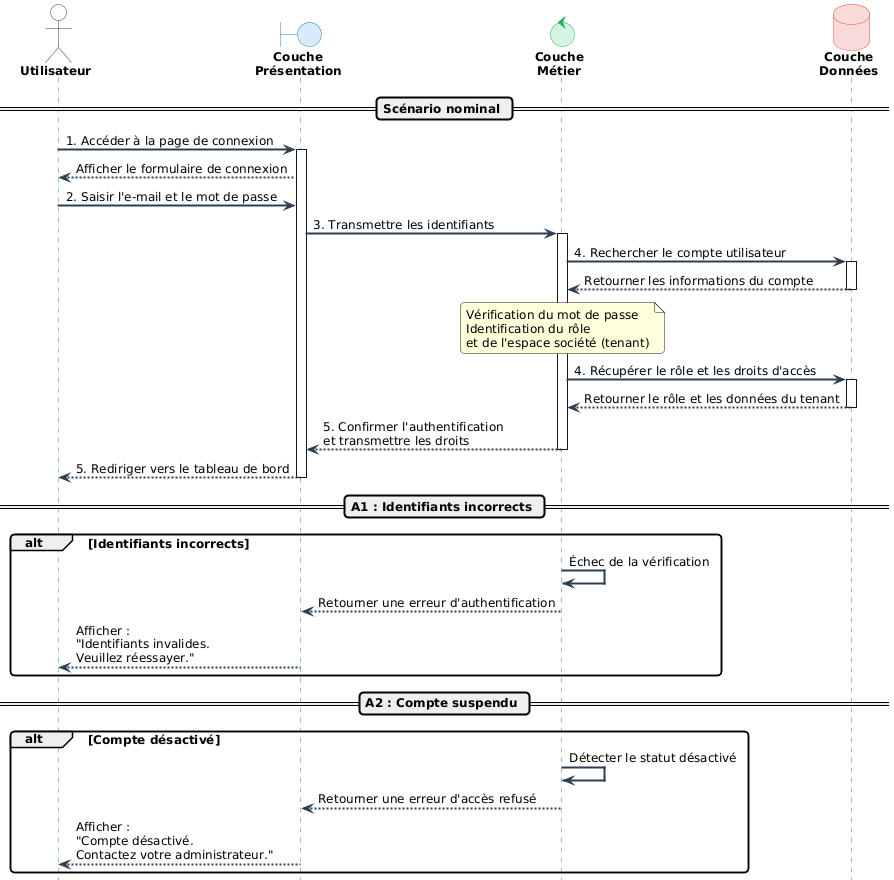
\includegraphics[width=0.99\textwidth]{seq-sp1-uc1.png}
    \caption{Diagramme de séquence — Authentification}
    \label{fig:seq-auth}
\end{figure}
\newpage

% -----------------------------------------------------------
\subsubsection{Diagramme de séquence : Création d'un utilisateur 
avec enregistrement d'audit}
% -----------------------------------------------------------
La figure~\ref{fig:seq-create-user} illustre le flux de création d'un utilisateur, incluant le déclenchement automatique de l'enregistrement dans le 
journal d'audit via l'interception AOP Spring. Le flux modélisé couvre~:

\vspace{1cm}

\begin{figure}[htbp]
    \centering
    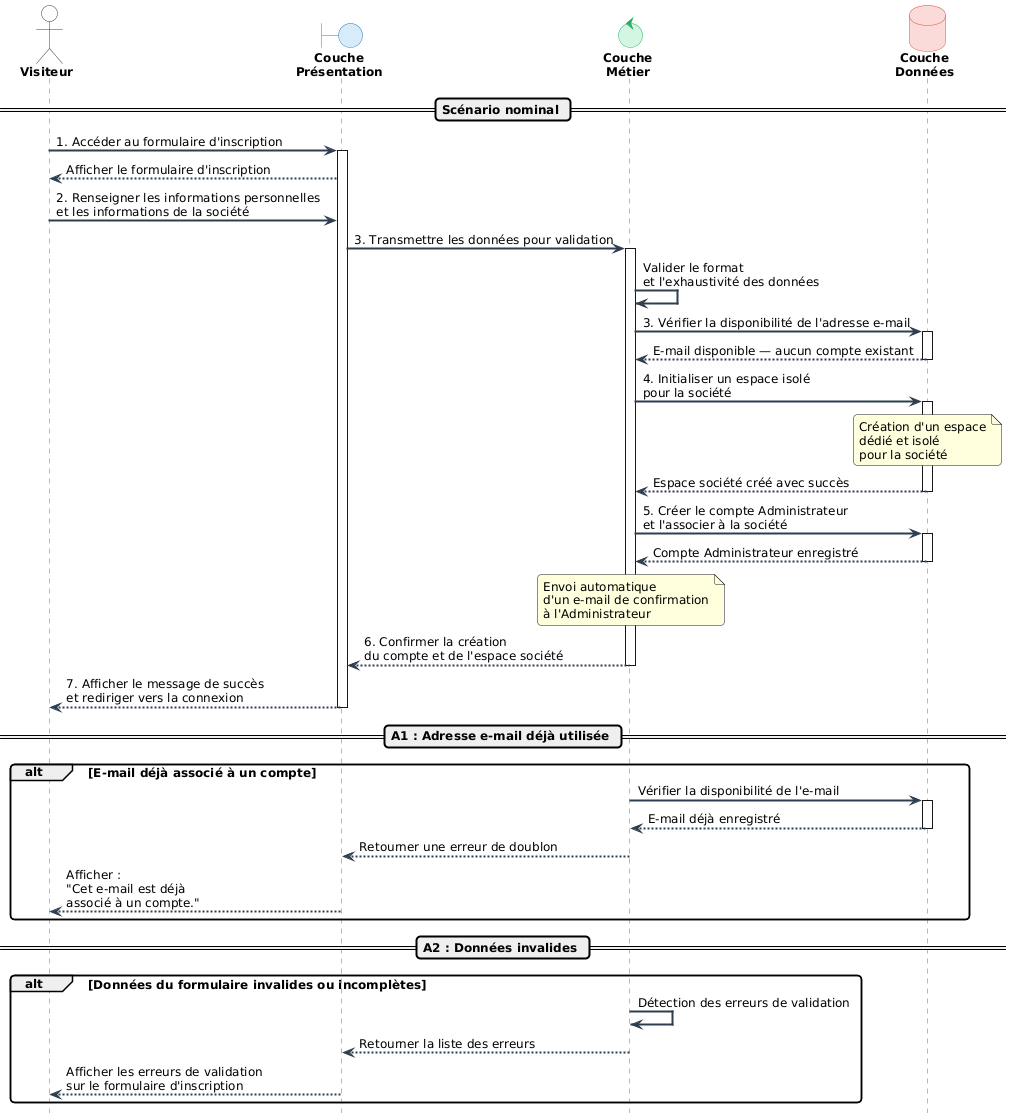
\includegraphics[width=0.99\textwidth]{seq-sp1-uc2.png}
    \caption{Diagramme de séquence — Création d'un utilisateur avec 
    enregistrement d'audit}
    \label{fig:seq-create-user}
\end{figure}

% ============================================================
\section{Réalisation du premier Sprint}
\label{sec:s1-realisation}
% ============================================================
Cette section détaille les réalisations concrètes du premier sprint, marquant le 
passage des spécifications à une solution logicielle fonctionnelle. Les travaux ont 
porté sur la mise en place de l'infrastructure technique, l'implémentation du socle 
de sécurité et le développement des premières interfaces utilisateurs. Cette étape 
matérialise la validation des User Stories prioritaires, notamment la gestion des 
accès et l'isolation des données, posant ainsi les fondations robustes de la 
plateforme PaieZone.

% -----------------------------------------------------------
\subsection{Inscription et initialisation de l'espace société}
% -----------------------------------------------------------
Le flux d'inscription de PaieZone est conçu pour permettre à un nouveau client 
(Visiteur) de créer simultanément son compte administrateur et l'espace isolé de 
sa société en une seule démarche guidée.

\begin{figure}[htbp]
    \centering
    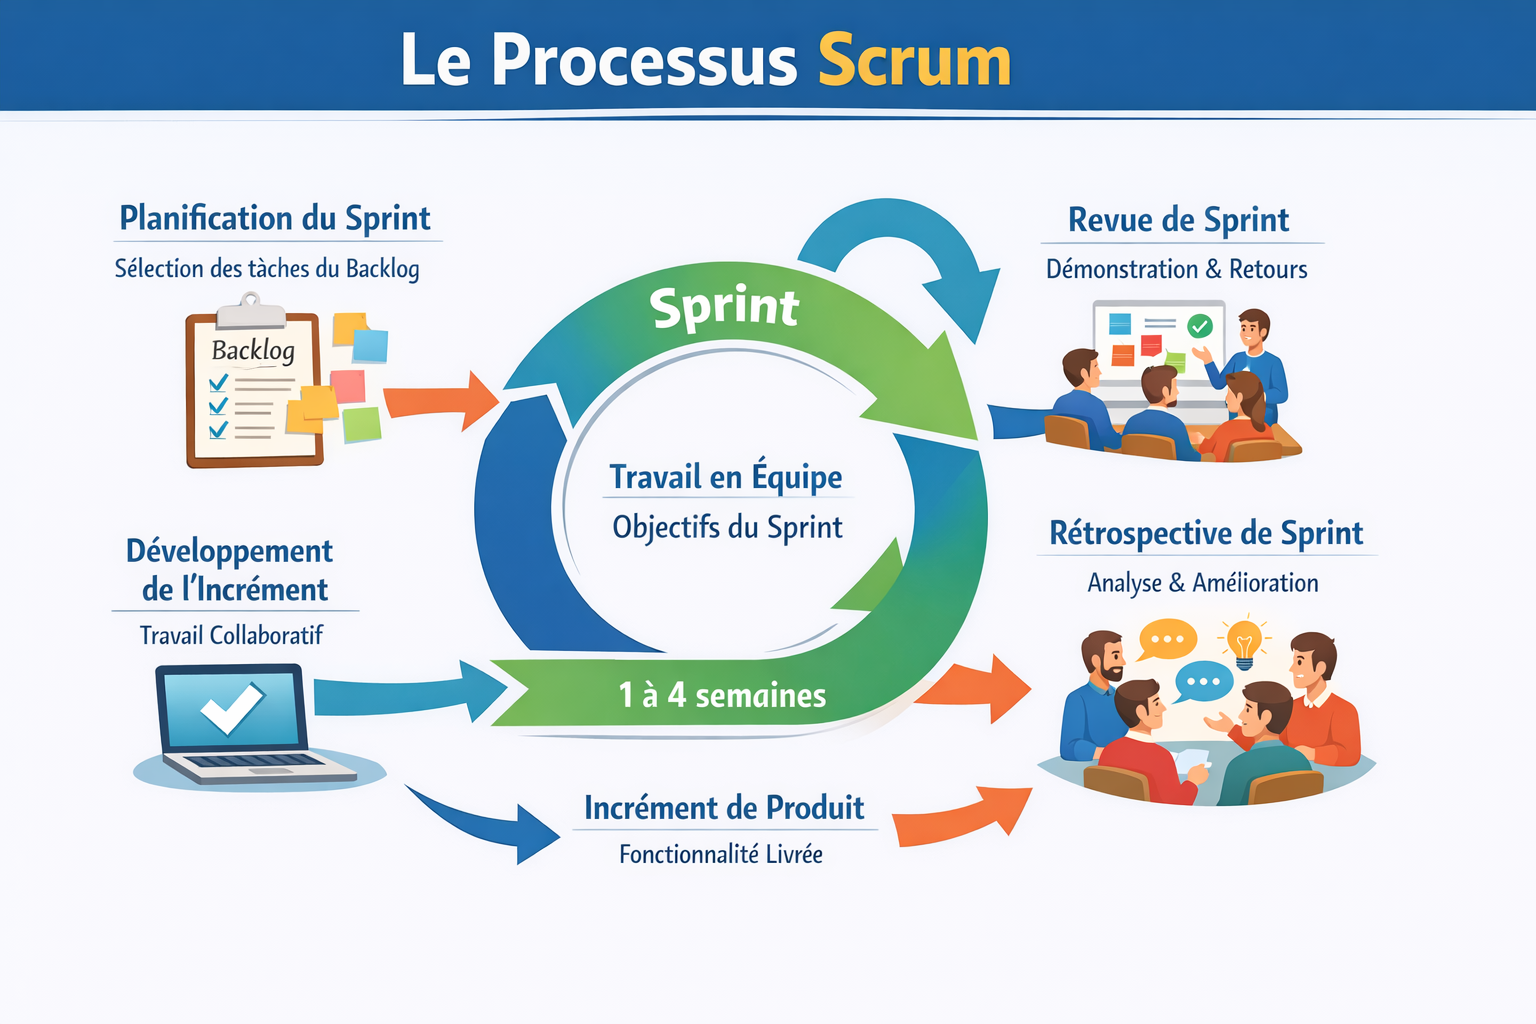
\includegraphics[width=0.7\textwidth]{scrum.png}
    \caption{Formulaire d'inscription — Informations personnelles et informations 
    de la société}
    \label{fig:ui-inscription}
\end{figure}

La figure~\ref{fig:ui-inscription} illustre le formulaire d'inscription, 
regroupant les données personnelles de l'administrateur et les informations légales 
de l'entreprise. La validation de ce formulaire déclenche automatiquement le 
provisionnement d'un schéma PostgreSQL dédié et l'application des migrations 
Liquibase, garantissant l'isolation complète des données de la société au sein de 
la base de données.

% -----------------------------------------------------------
\subsection{Authentification et accès}
% -----------------------------------------------------------
L'authentification constitue le point d'entrée unique de la plateforme PaieZone. 
Le système implémente un mécanisme de connexion sécurisé basé sur le standard JWT 
(JSON Web Token), complété par une redirection intelligente vers le tableau de bord 
correspondant au rôle de l'utilisateur connecté.

\begin{figure}[htbp]
    \centering
    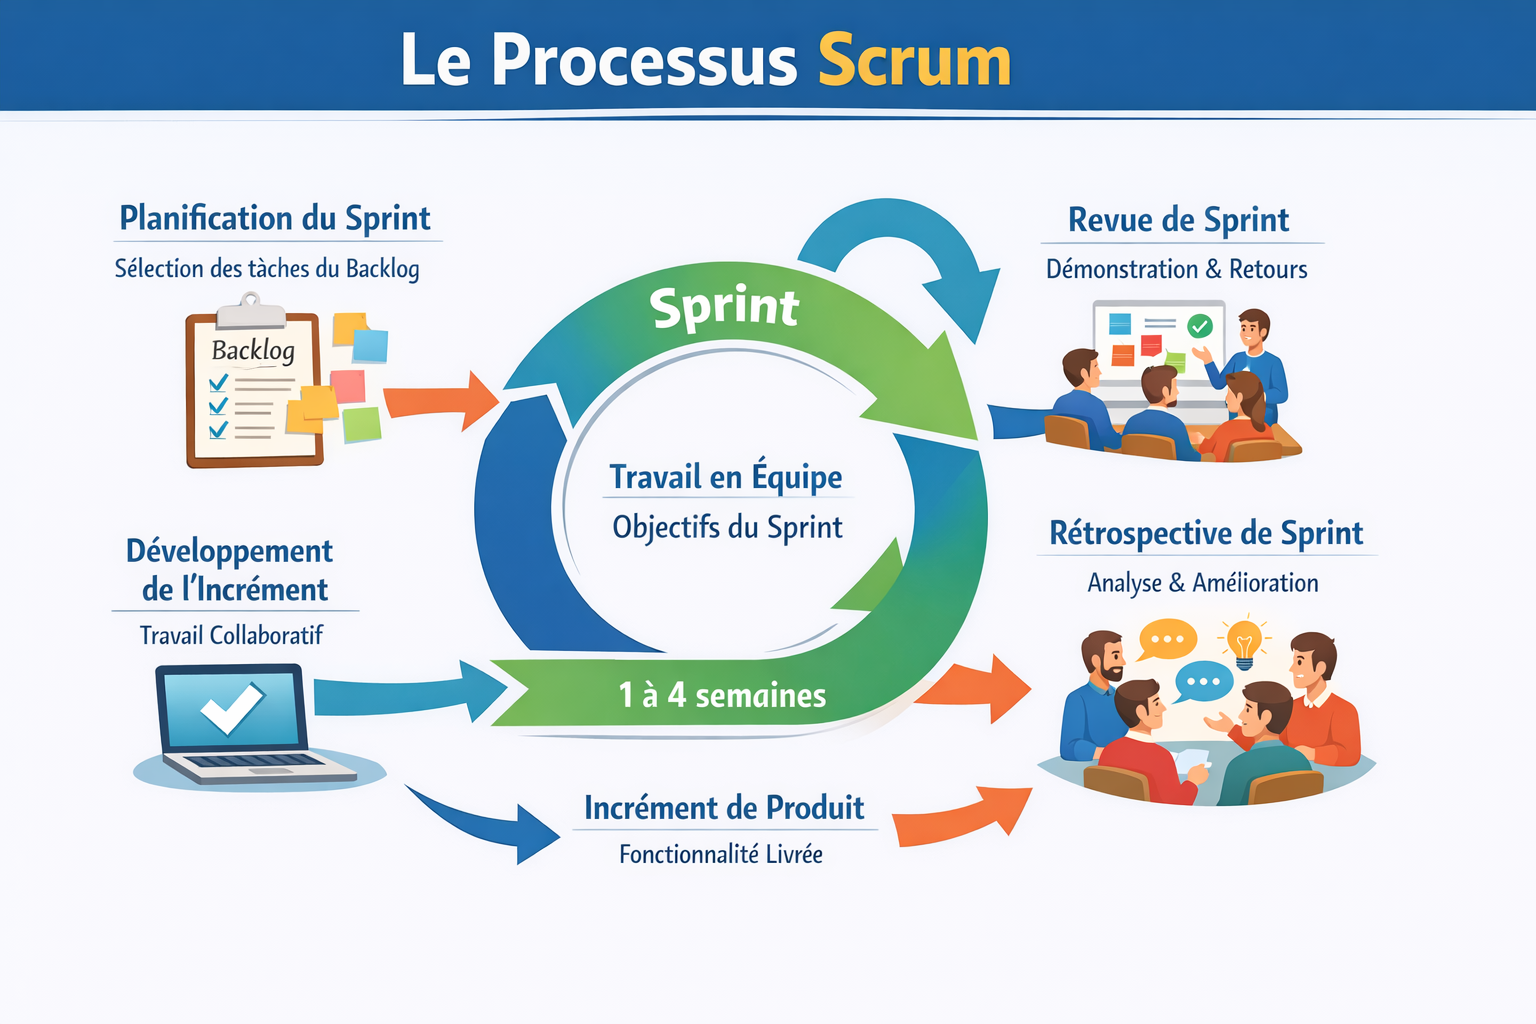
\includegraphics[width=0.75\textwidth]{scrum.png}
    \caption{Page de connexion de \pz}
    \label{fig:ui-login}
\end{figure}

La figure~\ref{fig:ui-login} présente la page de connexion d. Le formulaire 
collecte l'adresse e-mail et le mot de passe de l'utilisateur. En cas d'échec 
d'authentification, un message d'erreur générique est affiché, sans préciser si 
c'est l'e-mail ou le mot de passe qui est erroné, conformément aux bonnes pratiques 
de sécurité.

\begin{figure}[htbp]
    \centering
    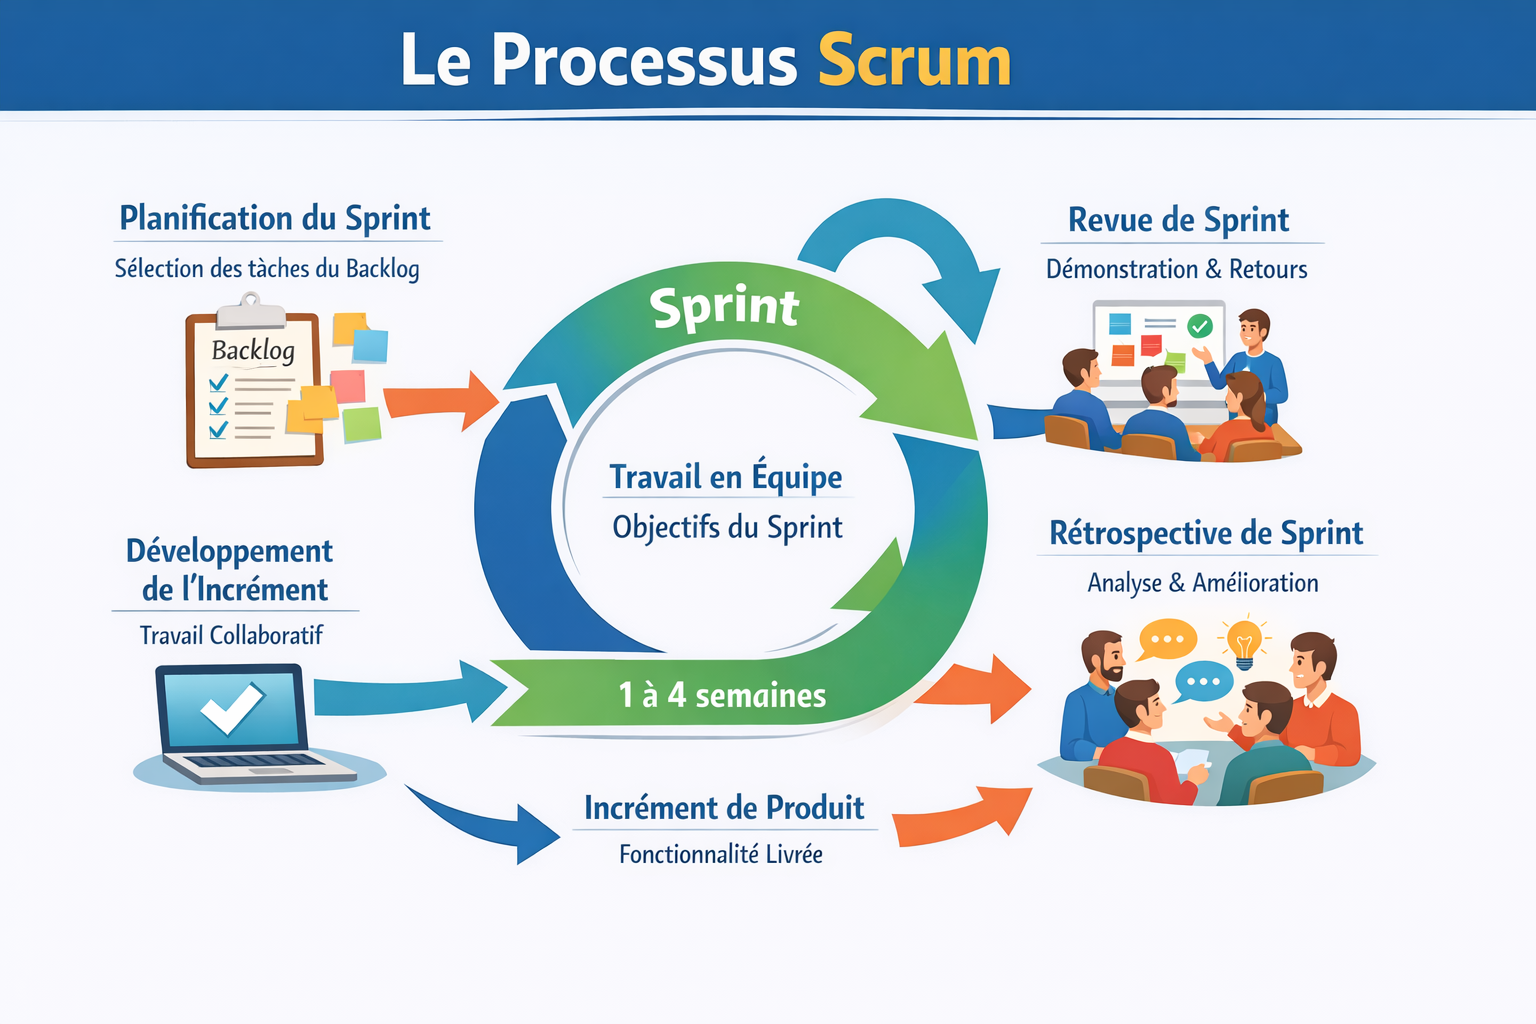
\includegraphics[width=0.75\textwidth]{scrum.png}
    \caption{Tableau de bord — Vue SuperAdmin après authentification}
    \label{fig:ui-dashboard-Superadmin}
\end{figure}

\begin{figure}[htbp]
    \centering
    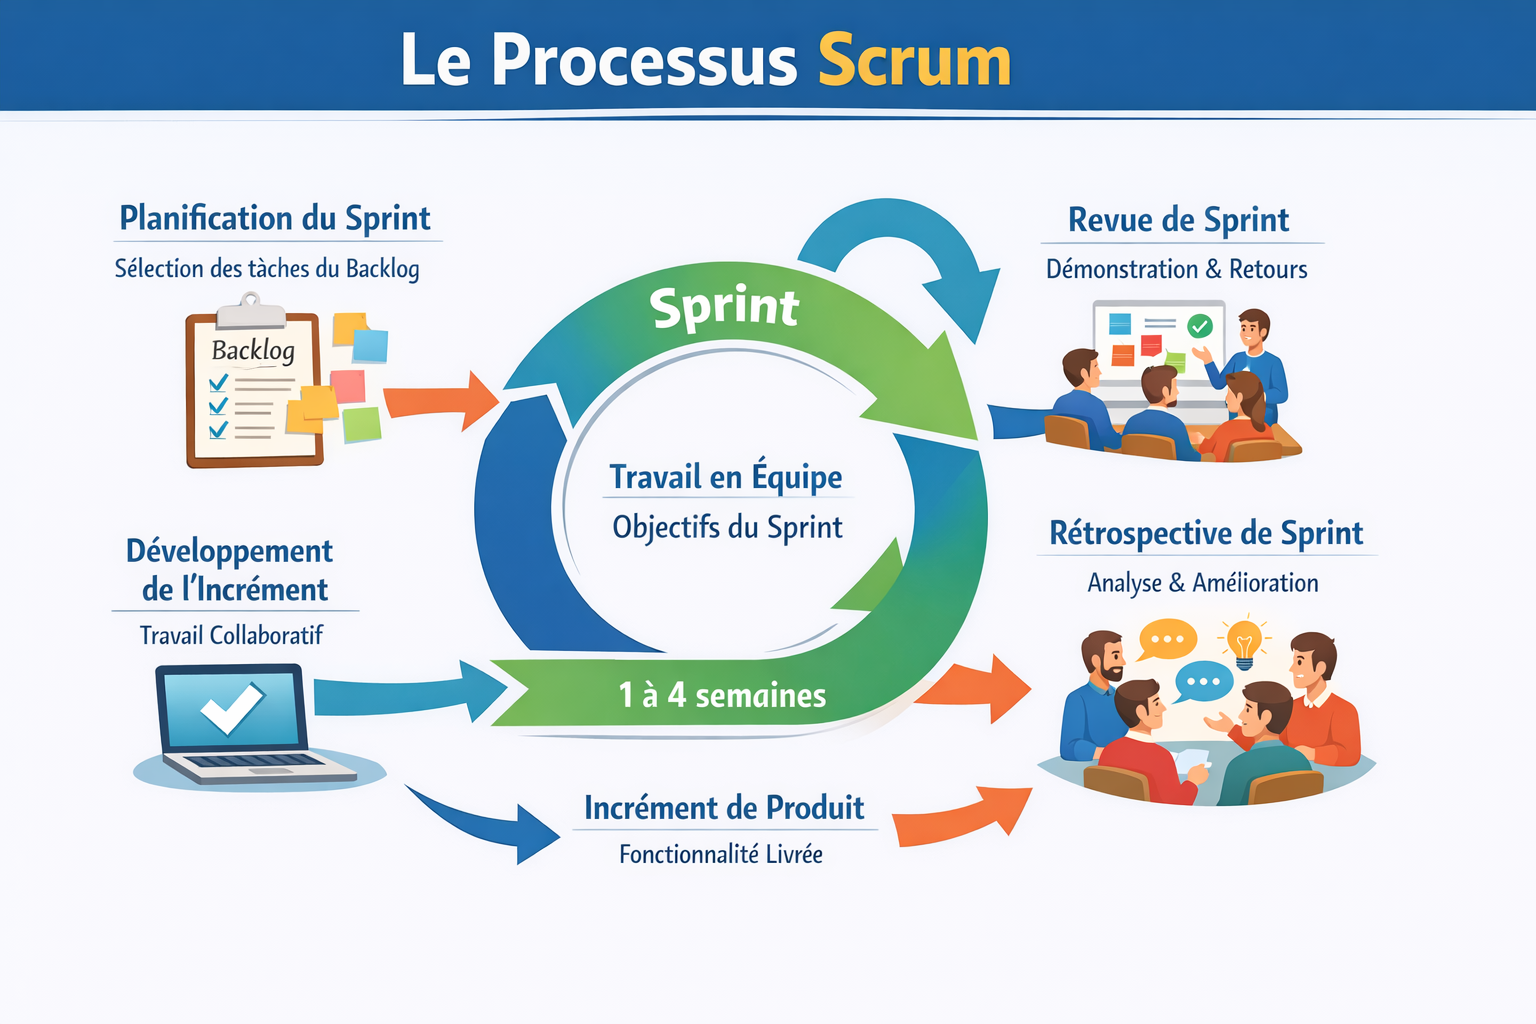
\includegraphics[width=0.75\textwidth]{scrum.png}
    \caption{Tableau de bord — Vue Administrateur après authentification}
    \label{fig:ui-dashboard-admin}
\end{figure}

\newpage

\begin{figure}[htbp]
    \centering
    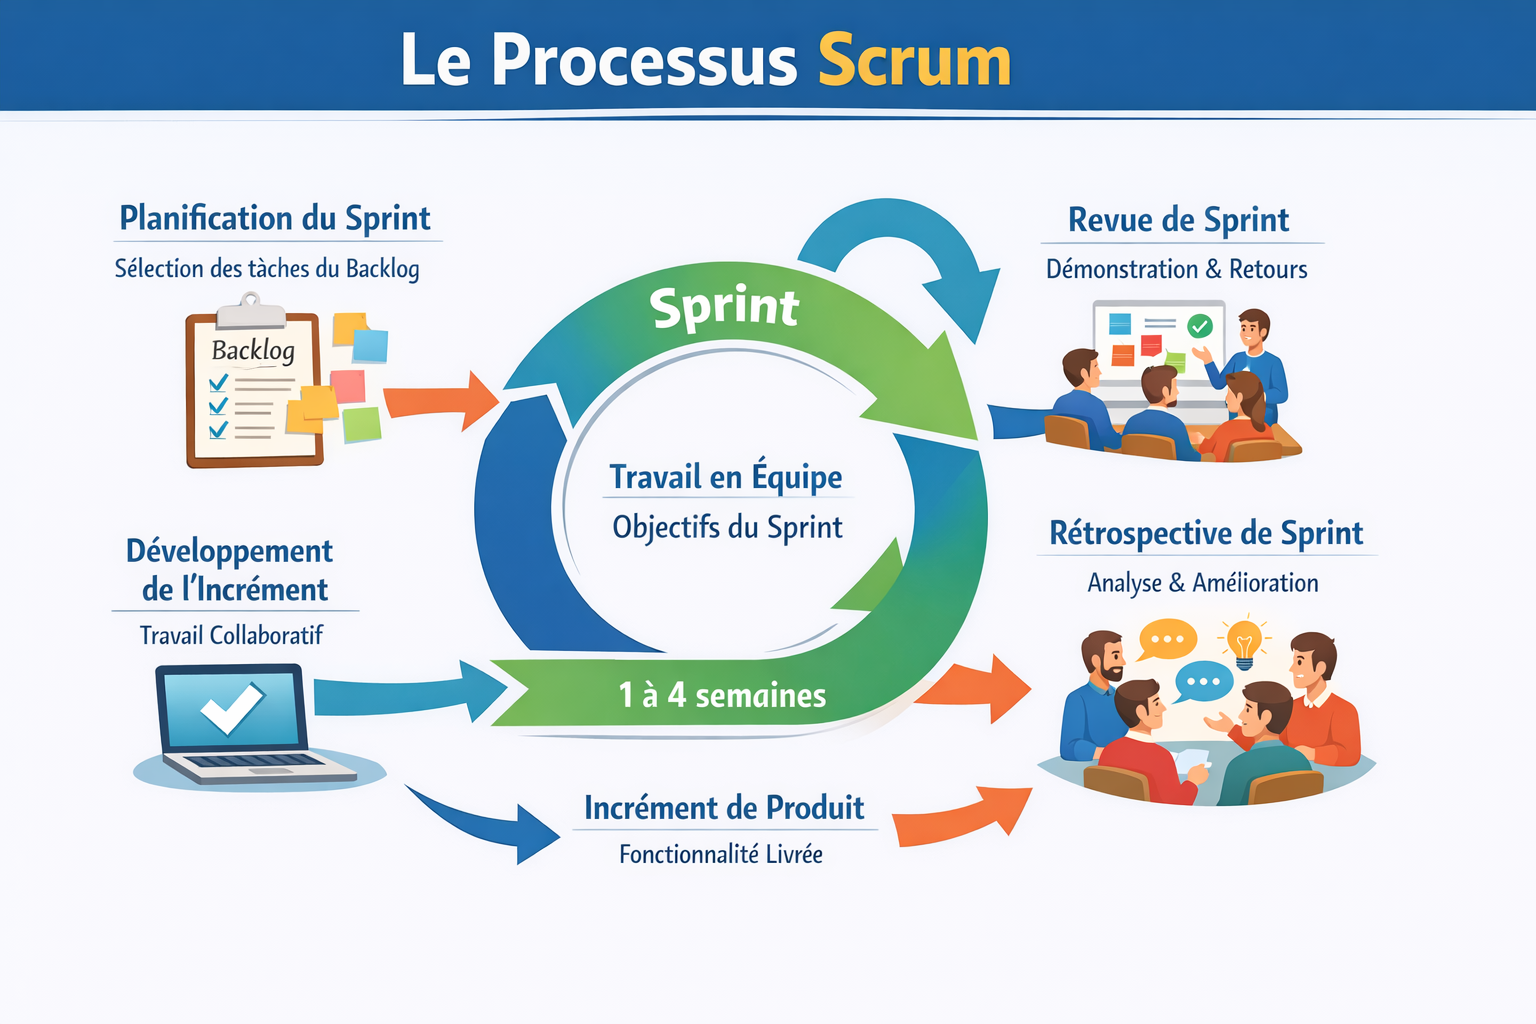
\includegraphics[width=0.75\textwidth]{scrum.png}
    \caption{Tableau de bord — Vue Employé après authentification}
    \label{fig:ui-dashboard-employe}
\end{figure}

\begin{figure}[htbp]
    \centering
    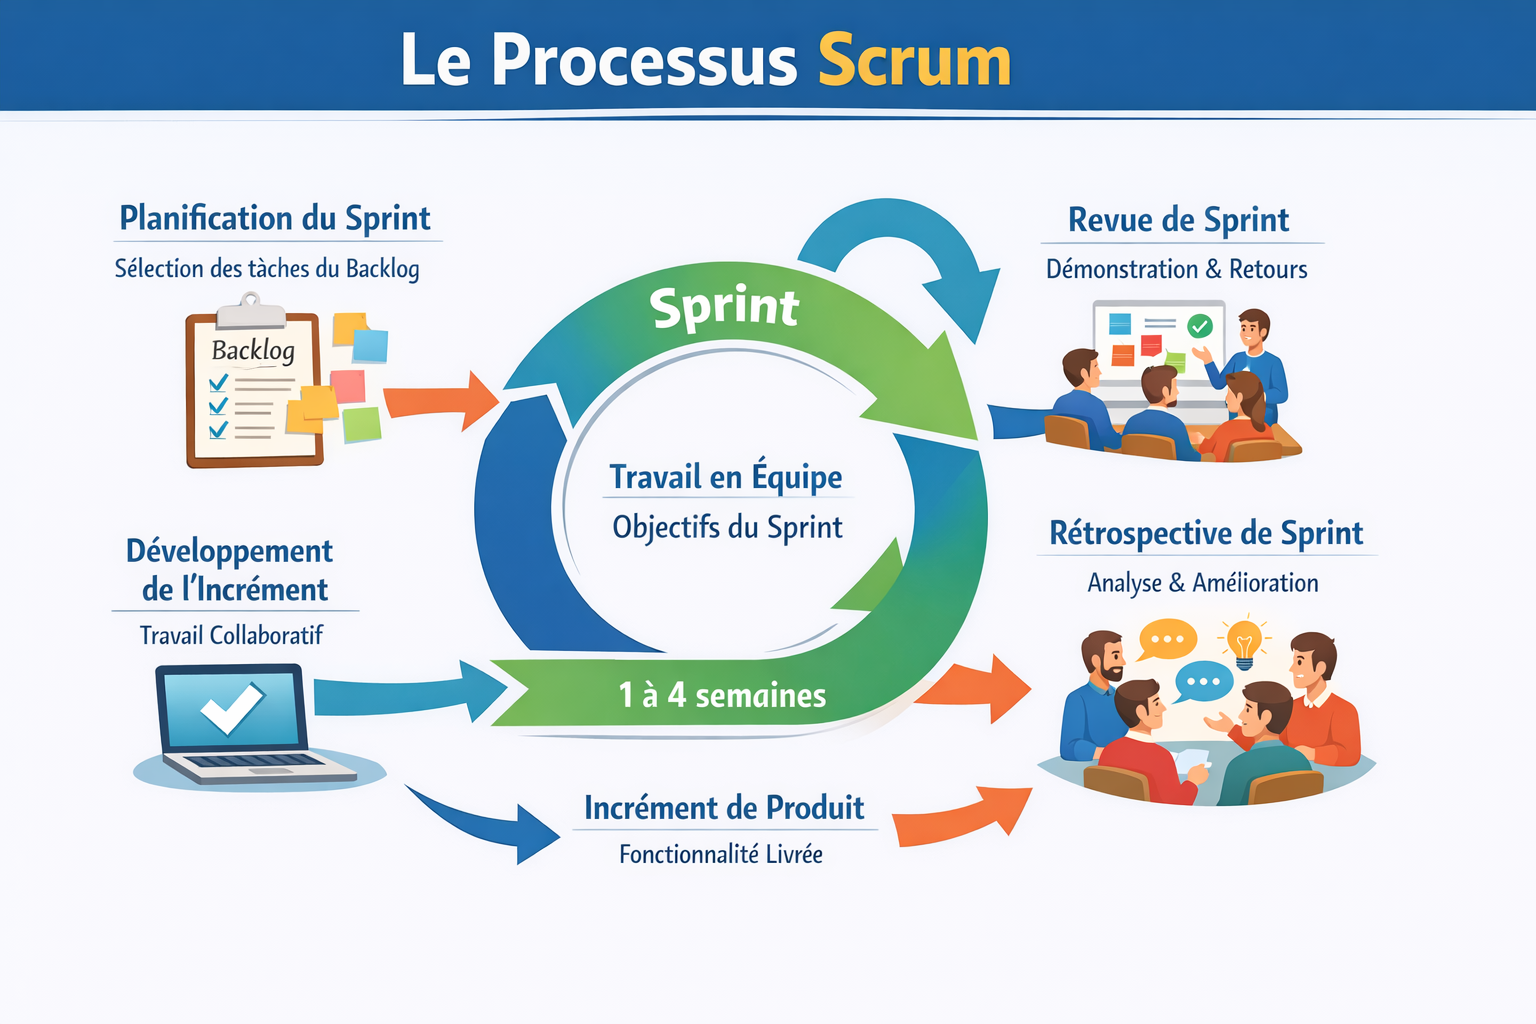
\includegraphics[width=0.75\textwidth]{scrum.png}
    \caption{Tableau de bord — Vue RH après authentification}
    \label{fig:ui-dashboard-rh}
\end{figure}

\newpage
Les figures \ref{fig:ui-dashboard-admin} à \ref{fig:ui-dashboard-rh} illustrent la redirection basée sur le modèle RBAC. Une fois authentifié, l'utilisateur est orienté vers un tableau de bord spécifique à son rôle (Super Admin, Admin, RH Comptable ou Employé), garantissant un accès sécurisé aux seuls modules autorisés.

% -----------------------------------------------------------
\subsection{Gestion des utilisateurs}
% -----------------------------------------------------------
Le module de gestion des utilisateurs, pilier central du premier sprint, permet à 
l'Administrateur de piloter l'ensemble des comptes collaborateurs (création, 
invitation, modification et désactivation).

\begin{figure}[htbp]
    \centering
    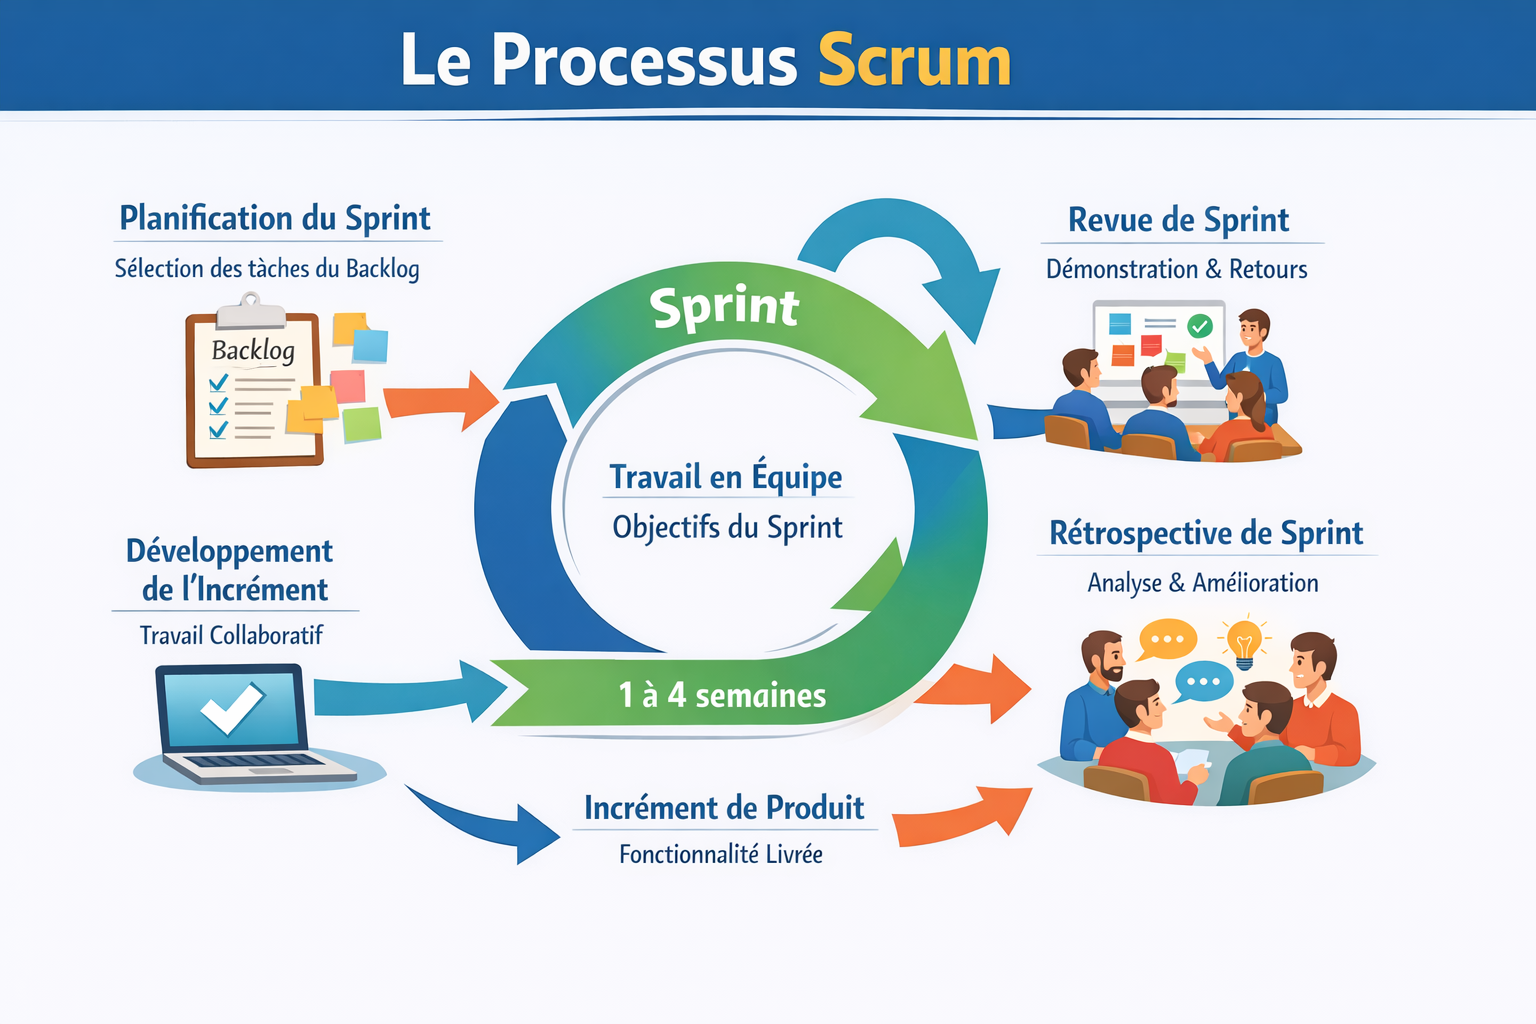
\includegraphics[width=0.70\textwidth]{scrum.png}
    \caption{Liste des utilisateurs}
    \label{fig:ui-users-list}
\end{figure}

\newpage
La figure~\ref{fig:ui-users-list} illustre l'interface de consultation, où les 
utilisateurs sont listés avec leurs informations clés~: identité, rôle et statut. 
Pour optimiser l'expérience de gestion, cette table intègre des fonctions de 
recherche et de pagination, facilitant la navigation au sein des effectifs de 
l'entreprise.

\begin{figure}[htbp]
    \centering
    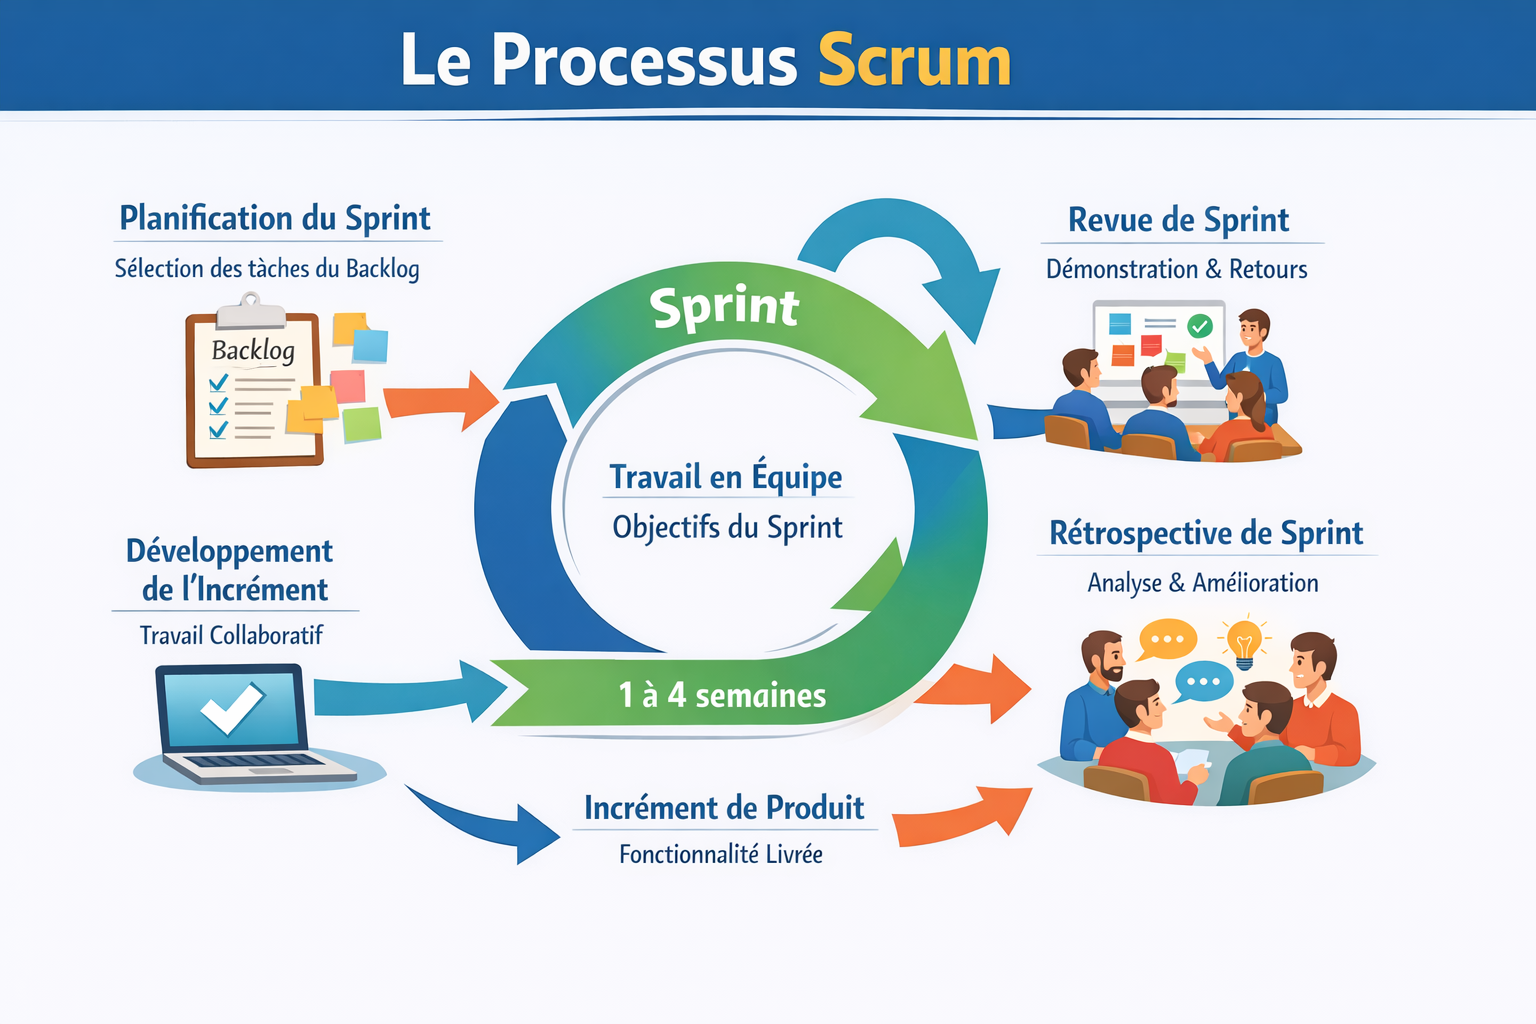
\includegraphics[width=0.7\textwidth]{scrum.png}
    \caption{Formulaire d'ajout et de modification d'un utilisateur}
    \label{fig:ui-users-form}
\end{figure}

La Figure \ref{fig:ui-users-form} illustre l'interface de gestion des profils où l'Administrateur renseigne les coordonnées et assigne les rôles. La cohérence des données est garantie par une double validation systématique 
% -----------------------------------------------------------
\subsection{Journal d'audit}
% -----------------------------------------------------------
Le module d'audit \ref{fig:ui-audit-list} assure la traçabilité complète en enregistrant automatiquement chaque action sensible. Pour chaque opération, le système archive l'identité de l'auteur, la nature de la modification (valeurs avant/après) et l'horodatage, garantissant ainsi l'intégrité et la surveillance du système.
\newpage
\begin{figure}[htbp]
    \centering
    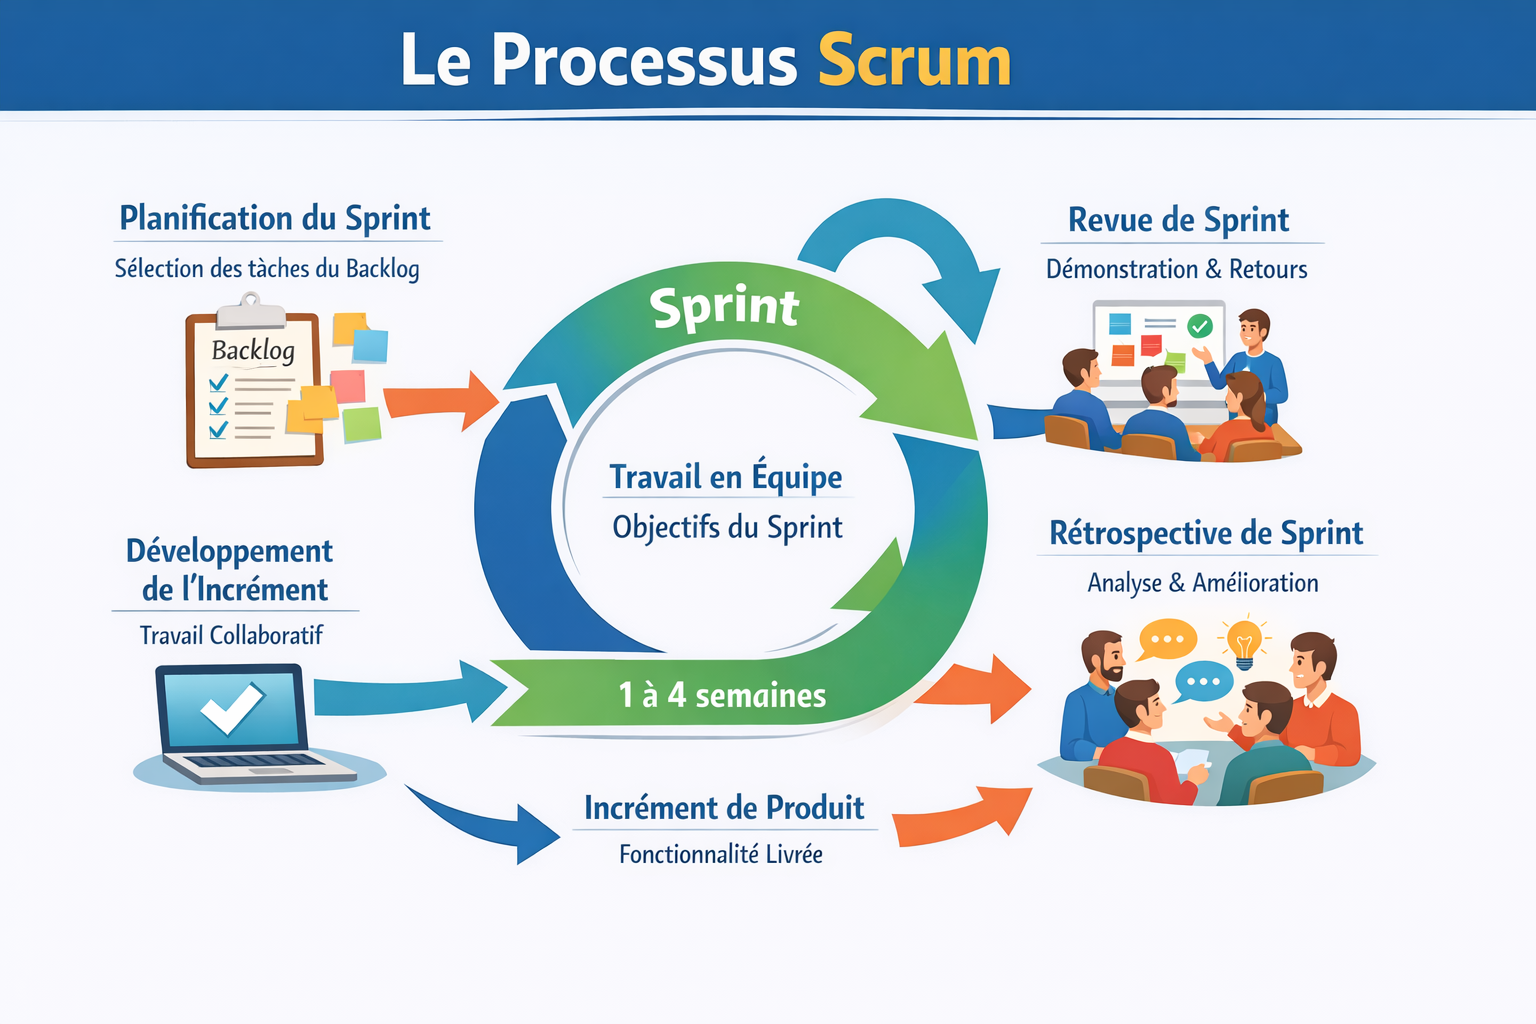
\includegraphics[width=0.70\textwidth]{scrum.png}
    \caption{Journal d'audit — Liste des actions enregistrées}
    \label{fig:ui-audit-list}
\end{figure}

La figure~\ref{fig:ui-audit-list} illustre l'interface de consultation du journal 
d'audit, accessible aux rôles Admin et RH. Les entrées peuvent être filtrées par 
date, par utilisateur et par type d'action, permettant un audit ciblé et rapide 
des événements système.

% -----------------------------------------------------------
\subsection{Gestion Organisationnelle}
% -----------------------------------------------------------
Le module de gestion organisationnelle permet aux Administrateurs 
et au RH de définir et de maintenir la structure hiérarchique de l'entreprise.

\begin{figure}[htbp]
    \centering
    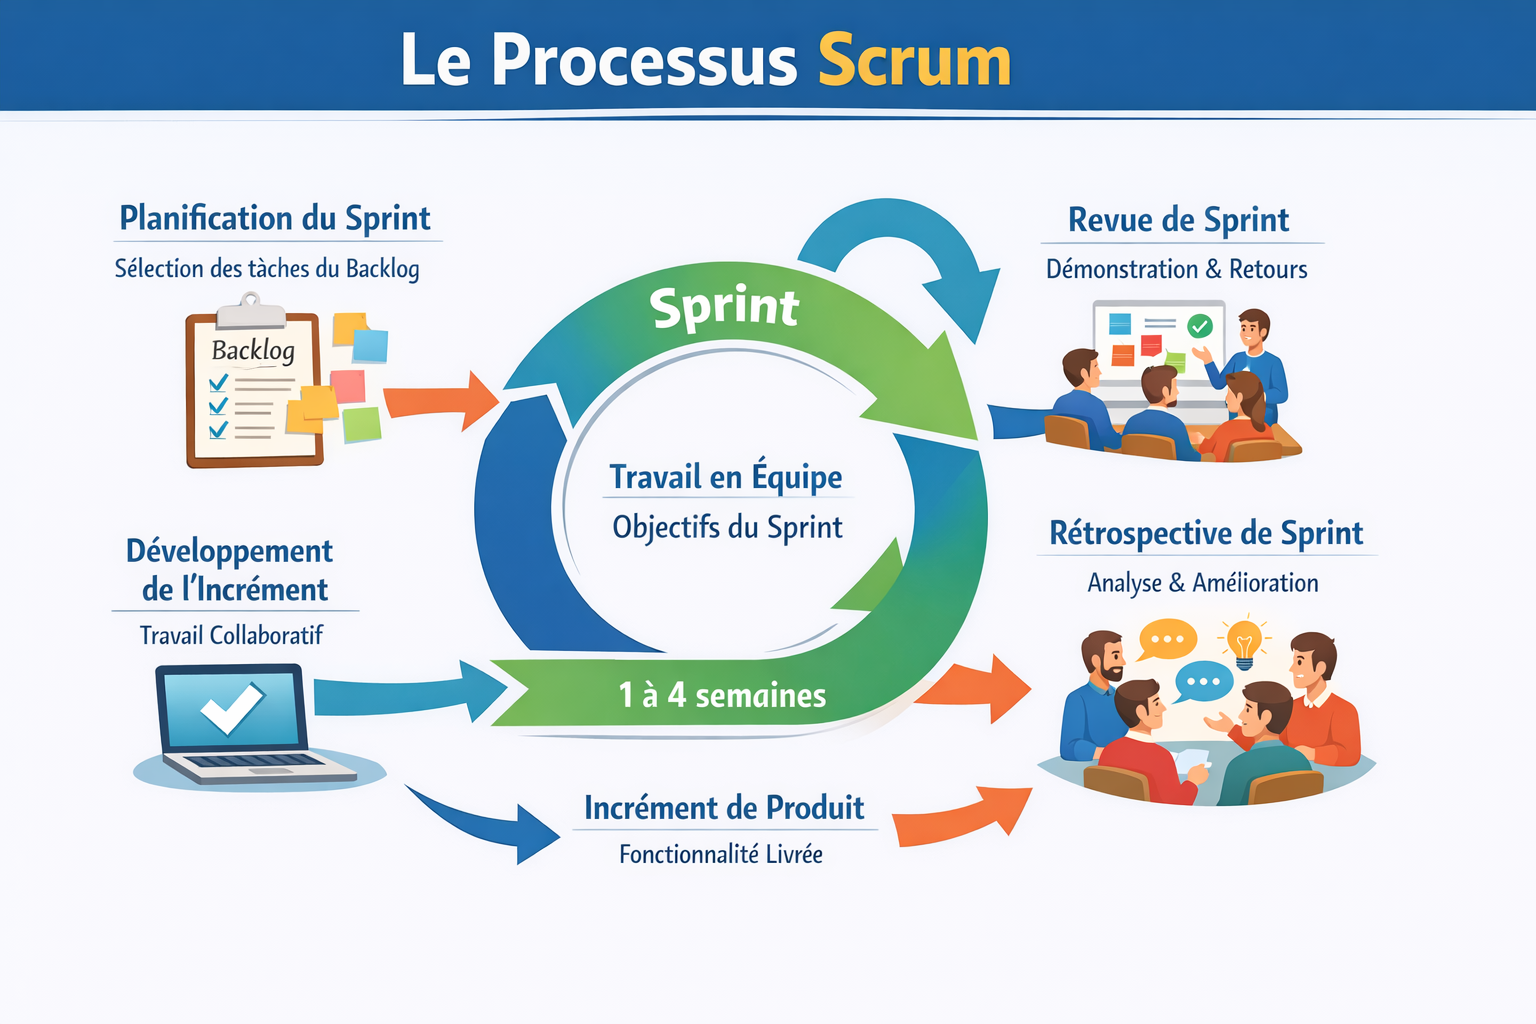
\includegraphics[width=0.70\textwidth]{scrum.png}
    \caption{Interface de gestion des départements et postes}
    \label{fig:ui-org}
\end{figure}

La Figure \ref{fig:ui-org} présente l'interface de gestion des départements et des postes. Elle permet aux administrateurs et RH de piloter la structure organisationnelle, tout en garantissant l'intégrité des données par un contrôle strict des dépendances lors de la désactivation d'un service.
% ============================================================
\section{Tests et Validation}
\label{sec:s1-tests}
% ============================================================
La phase de tests et de validation constitue une composante essentielle du cycle 
de développement agile. Elle vise à vérifier la conformité des fonctionnalités 
implémentées par rapport aux User Stories initialement définies, à identifier et 
corriger les anomalies avant la livraison au Product Owner, et à garantir la 
fiabilité, la robustesse et la qualité globale de la solution PaieZone.

% -----------------------------------------------------------
\subsection{Plan de tests}
% -----------------------------------------------------------
Afin de garantir la qualité logicielle du projet \pz, une stratégie de test 
multiniveaux a été adoptée lors du Sprint~1. Cette approche s'articule autour 
des axes suivants~:

\begin{itemize}[label=\textbullet, leftmargin=0.6cm]

    \item \textbf{Tests unitaires~:} Validation de la logique métier isolée, 
    notamment les mécanismes d'authentification JWT (génération, validation, 
    expiration du token), le Tenant Provisioning (création du schéma PostgreSQL) 
    et la génération des tokens d'invitation.

    \item \textbf{Tests d'intégration~:} Vérification de la cohérence des flux 
    entre les couches applicatives et la base de données de test~: inscription 
    multi-tenant avec isolation des schémas, persistance des journaux d'audit 
    et contrôle des accès RBAC.

    \item \textbf{Tests fonctionnels~:} Évaluation du comportement des interfaces 
    Angular~: formulaires d'inscription et de connexion, gestion des erreurs de 
    validation, redirection différenciée par rôle et filtrage du journal d'audit.
\end{itemize}

Cette approche rigoureuse garantit la fiabilité technique de la solution ainsi que sa conformité aux besoins métiers identifiés. Le Tableau \ref{tab:tests-sprint1} récapitule les principaux scénarios de test exécutés durant ce sprint pour valider ces exigences.

\renewcommand{\arraystretch}{1.3}
\begin{small}
\begin{xltabular}{\textwidth}{|c|>{\raggedright\arraybackslash}X|>{\raggedright\arraybackslash}p{4cm}|c|}
\hline
\rowcolor[gray]{0.9}
\textbf{ID} & \textbf{Description} & \textbf{Résultat attendu} & \textbf{Statut} \\
\hline
\endfirsthead
\hline
\rowcolor[gray]{0.9}
\textbf{ID} & \textbf{Description} & \textbf{Résultat attendu} & \textbf{Statut} \\
\hline
\endhead
\hline
\endfoot
\hline
\caption{Récapitulatif des cas de test du Sprint~1}
\label{tab:tests-sprint1}
\endlastfoot

T-1.1 & Authentification avec identifiants valides
& Token JWT généré, redirection vers le tableau de bord du rôle
& \textcolor{green!60!black}{\textbf{OK}} \\ \hline
T-1.2 & Authentification avec un compte désactivé ou identifiants invalides
& Accès refusé, message d'erreur générique affiché
& \textcolor{green!60!black}{\textbf{OK}} \\ \hline
T-1.3 & Authentification avec code 2FA invalide (Super Admin)
& Accès refusé, invitation à ressaisir le code TOTP
& \textcolor{green!60!black}{\textbf{OK}} \\ \hline
T-2.1 & Inscription d'une nouvelle entreprise (Tenant Provisioning)
& Schéma PostgreSQL créé, migrations Liquibase appliquées
& \textcolor{green!60!black}{\textbf{OK}} \\ \hline
T-2.2 & Inscription avec un matricule fiscal déjà enregistré
& Blocage avec message d'erreur explicite
& \textcolor{green!60!black}{\textbf{OK}} \\ \hline
T-3.1 & Création d'un utilisateur avec attribution de rôle
& Compte persisté en base avec les droits associés
& \textcolor{green!60!black}{\textbf{OK}} \\ \hline
T-3.2 & Envoi d'une invitation par e-mail et acceptation
& Token généré, e-mail envoyé, compte activé après définition du mot de passe
& \textcolor{green!60!black}{\textbf{OK}} \\ \hline
T-3.3 & Désactivation d'un utilisateur actif
& Accès révoqué immédiatement, statut mis à jour en base
& \textcolor{green!60!black}{\textbf{OK}} \\ \hline
T-4.1 & Enregistrement automatique des actions dans le journal d'audit
& Entrée créée avec (action, entité, auteur, IP, date, valeurs avant/après)
& \textcolor{green!60!black}{\textbf{OK}} \\ \hline
T-5.1 & Création d'un département et d'un poste rattaché
& Structure organisationnelle mise à jour avec succès
& \textcolor{green!60!black}{\textbf{OK}} \\ \hline
T-5.2 & Tentative de désactivation d'un département contenant des postes actifs
& Désactivation bloquée, message d'alerte affiché
& \textcolor{green!60!black}{\textbf{OK}} \\ \hline
\end{xltabular}
\end{small}
\renewcommand{\arraystretch}{1.0}

% -----------------------------------------------------------
\subsection{Tests automatisés}
% -----------------------------------------------------------

Afin de renforcer la fiabilité du Sprint~1, des tests automatisés ont été
mis en place pour valider les deux composantes les plus critiques de cette
itération~: l'isolation multi-tenant et la sécurité des accès.

\paragraph{Tests unitaires --- TenantContextService (JUnit~5 + Mockito)}
Le service \texttt{TenantContextService} est le gardien de l'architecture
multi-tenant de \pz{}~: il résout le \texttt{companyId} de chaque utilisateur
connecté et filtre toutes les requêtes JPA en conséquence. Quatorze cas de test
ont été écrits et exécutés~:

\begin{itemize}[label=\textbullet, leftmargin=0.6cm, itemsep=2pt]
    \item \textbf{Super Admin~:} \texttt{getCurrentCompanyId()} retourne \texttt{null}
    (accès global, aucun filtre appliqué sur les données).
    \item \textbf{Admin avec profil~:} le \texttt{companyId} est correctement résolu
    depuis son \texttt{UserProfile} en base.
    \item \textbf{Fallback~:} sans \texttt{UserProfile}, résolution via le champ
    \texttt{adminLogin} de la table \texttt{Company}.
    \item \textbf{Fail-closed~:} un utilisateur sans entreprise résolue reçoit
    \texttt{companyId = -1L}, bloquant tout accès aux données --- aucune fuite
    par défaut.
    \item \textbf{Accès croisé~:} \texttt{canAccessCompany(autreId)} retourne
    \texttt{false} pour toute entreprise n'appartenant pas à l'utilisateur.
\end{itemize}

\textbf{Résultat~:} 14/14 tests passés (\textcolor{green!60!black}{\textbf{OK}}).

\paragraph{Tests End-to-End --- Cypress}
Des scénarios Cypress ont automatisé la vérification de la couche sécurité~:
connexion avec identifiants valides (redirection vers le tableau de bord du rôle),
connexion échouée (maintien sur la page login), accès direct à \texttt{/paiezone/saas-dash}
sans authentification (redirection vers login), et vérification que les endpoints
\texttt{/api/companies} et \texttt{/api/dashboard/stats} retournent HTTP~401 sans token.

% ============================================================
\section{Rituels Agiles et Clôture du Sprint}
\label{sec:s1-rituels}
% ============================================================
La méthodologie Scrum impose, à la fin de chaque sprint, la tenue de deux rituels 
essentiels~: la Sprint Review et la Sprint Retrospective. Ces cérémonies garantissent 
la transparence et l'amélioration continue au sein de l'équipe PaieZone, en 
permettant respectivement d'inspecter le travail accompli et d'adapter les pratiques 
pour le sprint suivant.

% -----------------------------------------------------------
\subsection{Revue du Sprint (Sprint Review)}
% -----------------------------------------------------------

La Sprint Review a réuni l'équipe de développement, le Product Owner et les parties
prenantes. Les démonstrations ont couvert le flux d'authentification avec provisionnement
multi-tenant, la gestion des départements et postes, le journal d'audit ainsi que
l'interface Super Admin de gestion des abonnements SaaS. L'ensemble des 19 User Stories
planifiées a été validé par le Product Owner, confirmant la conformité des livrables
aux critères d'acceptation.

% -----------------------------------------------------------
\subsection{Rétrospective du Sprint (Sprint Retrospective)}
% -----------------------------------------------------------

La rétrospective a permis à l'équipe de réfléchir sur trois axes :

\begin{itemize}
    \item \textbf{Ce qui a bien fonctionné :}
    Une bonne collaboration entre les équipes front-end et back-end, assurant
    une intégration fluide et une traçabilité complète des actions.

    \item \textbf{Problèmes rencontrés :}
    La mise en place du multi-tenant s'est révélée plus complexe que prévu,
    retardant légèrement les tests d'intégration.

    \item \textbf{Actions d'amélioration :}
    Anticiper les tâches techniques en début de sprint et renforcer
    les tests d'intégration pour détecter les anomalies plus tôt.
\end{itemize}

% ============================================================
\section*{Conclusion}
\label{sec:s1-conclusion}
\addcontentsline{toc}{section}{Conclusion}
% ============================================================
Ce chapitre a présenté la réalisation du Sprint~1 de PaieZone~RH,
qui marque l'établissement du socle technique et fonctionnel de la
  plateforme. Les dix-neuf User Stories validées (authentification
  sécurisée , Tenant Provisioning, gestion des abonnements
  SaaS, administration des utilisateurs avec flux d'invitation, journal
  d'audit automatique et structuration organisationnelle )constituent
  les fondations sur lesquelles s'appuieront tous les sprints ultérieurs.

  La cohérence entre la conception UML, les interfaces Angular livrées
  et les entités JPA garantit
  une architecture robuste et extensible. Le chapitre suivant présente
  les travaux du Sprint~2, consacré à la gestion du capital humain~:
  création et administration des dossiers employés, cycle de vie des
  contrats de travail et gestion documentaire.

% ==========================================
% CHAPITRE 4
% ==========================================
\newpage
\chapter{Étude et Réalisation du Deuxième Sprint}
\vspace{2.5cm}

\noindent \textbf{\Large Plan}
\vspace{0.8cm}

\begin{enumerate}[label=\textbf{\arabic*}, leftmargin=1.5cm, labelsep=0.8cm]
    \item[] \hspace*{-1.5cm}\textbf{Introduction}                          \dotfill \pageref{sec:s2-intro}
    \item \textbf{User Stories du deuxième sprint}       \dotfill \pageref{sec:s2-userstories}
    \item \textbf{Backlog du deuxième Sprint}            \dotfill \pageref{sec:s2-backlog}
    \item \textbf{Spécification fonctionnelle}           \dotfill \pageref{sec:s2-specification}
    \item \textbf{Conception du deuxième Sprint}         \dotfill \pageref{sec:s2-conception}
    \item \textbf{Étude et réalisation}                  \dotfill \pageref{sec:s2-realisation}
    \item \textbf{Tests et Validation}                   \dotfill \pageref{sec:s2-tests}
    \item \textbf{Rituels Agiles et Clôture du Sprint}   \dotfill \pageref{sec:s2-rituels}
    \item[] \hspace*{-1.5cm}\textbf{Conclusion}                            \dotfill \pageref{sec:s2-conclusion}
\end{enumerate}

\vfill
\newpage

% ============================================================
\section*{Introduction}
\label{sec:s2-intro}
\addcontentsline{toc}{section}{Introduction}
% ============================================================

S'appuyant sur les bases techniques consolidées lors du premier sprint, ce chapitre expose les réalisations du Sprint 2, véritable pivot opérationnel de la plateforme PaieZone RH. Cette itération est dédiée à la gestion du capital humain, intégrant l'administration des dossiers collaborateurs, le pilotage des cycles contractuels et la dématérialisation des documents administratifs. La méthodologie demeure rigoureuse : elle s'articule autour de la spécification par User Stories, d'une modélisation UML approfondie (classes et séquences), du développement des interfaces Angular, et se conclut par une phase de validation stricte suivie des rituels agiles de clôture.

% ============================================================
\section{User Stories du deuxième sprint}
\label{sec:s2-userstories}
% ============================================================

Lors de la réunion de planification du Sprint~2, l'équipe Scrum a défini
l'objectif du sprint autour de la valeur métier suivante~: «~Permettre à
l'équipe RH de gérer l'intégralité du dossier administratif d'un employé,
de son recrutement à la formalisation de sa relation contractuelle~». Trois
épics prioritaires ont été sélectionnés dans le backlog produit~:

\begin{itemize}[label=\textbullet, leftmargin=0.6cm]
    \item Gestion du Capital Humain
    \item Gestion du Cycle de Vie des Contrats de Travail
    \item Gestion des Documents Administratifs
\end{itemize}

Les besoins fonctionnels ont été formalisés sous forme de User Stories
détaillées dans le Tableau~\ref{tab:user-stories-sprint2}.
\renewcommand{\arraystretch}{1.4}
\begin{small}
\begin{longtable}{|p{1.2cm}|p{9.5cm}|p{2.3cm}|}

\hline
\rowcolor[gray]{0.9}
\textbf{ID} & \textbf{User Story} & \textbf{Priorité} \\
\hline
\endfirsthead

\hline
\rowcolor[gray]{0.9}
\textbf{ID} & \textbf{User Story} & \textbf{Priorité} \\
\hline
\endhead

\hline
\endfoot
\endfoot

6.1 & En tant qu'Admin/RH, je veux consulter la liste des employés,
      afin d'avoir une vue d'ensemble du personnel.
    & Haute \\ \hline

6.2 & En tant qu'Admin/RH, je veux créer un employé, afin de l'ajouter
      au système avec toutes ses données administratives et fiscales.
    & Critique \\ \hline

6.3 & En tant qu'Admin/RH, je veux consulter le profil d'un employé,
      afin de voir son dossier complet (informations, contrats,
      documents, historique).
    & Haute \\ \hline

6.4 & En tant qu'Admin/RH, je veux modifier un employé, afin de mettre
      à jour ses données personnelles ou contractuelles.
    & Haute \\ \hline

6.5 & En tant qu'Admin/RH, je veux désactiver un employé, afin de
      gérer sa sortie de l'organisation.
    & Haute \\ \hline

7.1 & En tant que RH, je veux associer un contrat à un employé, afin
      de formaliser la relation de travail (CDI, CDD, CIVP, KARAMA,
      Intérimaire ou Stage).
    & Critique \\ \hline

7.2 & En tant que RH, je veux modifier un contrat, afin de mettre à
      jour ses conditions avant résiliation.
    & Haute \\ \hline

7.3 & En tant que RH, je veux résilier un contrat, afin de terminer
      formellement une relation de travail.
    & Haute \\ \hline

8.1 & En tant que RH, je veux déposer un document administratif dans
      le dossier d'un employé, afin de constituer son dossier numérique.
    & Moyenne \\ \hline
\caption{User Stories du deuxième Sprint}   
\label{tab:user-stories-sprint2}    
\end{longtable}
\end{small}
\renewcommand{\arraystretch}{1.0}

% ============================================================
\section{Backlog du deuxième Sprint}
\label{sec:s2-backlog}
% ============================================================

Le Backlog du produit est formalisé en User Stories organisées
par thèmes fonctionnels. Le Tableau~\ref{tab:backlog-sprint2} détaille ce
backlog pour le deuxième sprint, incluant les tâches techniques et leurs
estimations en jours.

\begin{small}
\renewcommand{\arraystretch}{1.4}
\setlength{\LTleft}{\fill}
\setlength{\LTright}{\fill}
\begin{longtable}{|p{2.5cm}|p{6.0cm}|p{6.0cm}|c|}
\hline
\rowcolor[gray]{0.9} \textbf{Item} & \textbf{User Story} & \textbf{Tâches} & 
\makecell{\textbf{Est.}\\\textbf{(j)}} \\ \hline
\endfirsthead

\hline
\rowcolor[gray]{0.9} \textbf{Item} & \textbf{User Story} & \textbf{Tâches} & 
\makecell{\textbf{Est.}\\\textbf{(j)}} \\ \hline
\endhead
\hline
\endfoot
\hline
\caption{Backlog détaillé du deuxième Sprint}
\label{tab:backlog-sprint2}
\endlastfoot
% ── Gestion du Capital Humain ─────────────────────────────
\multirow{5}{*}{\makecell[c]{\textbf{Gestion du}\\ \textbf{Capital}\\ \textbf{Humain}}}
& \textbf{6.1} En tant qu'Admin/RH, je souhaite consulter la liste des
  employés afin d'avoir une vue d'ensemble du personnel.
& \begin{itemize}[leftmargin=*, noitemsep, topsep=0pt]
    \item Concevoir l'interface de la liste des employés (tableau paginé
          avec filtres et recherche).
    \item Développer l'API REST de récupération des employés liés à la
          société.
  \end{itemize}
& \textbf{1} \\ \cline{2-4}

& \textbf{6.2} En tant qu'Admin/RH, je souhaite créer un employé afin
  de l'ajouter au système.
& \begin{itemize}[leftmargin=*, noitemsep, topsep=0pt]
    \item Développer le formulaire de création du profil employé
          (informations personnelles, données fiscales et sociales,
          poste, département).
    \item Implémenter la génération automatique du matricule unique.
    \item Développer l'API REST d'insertion de l'employé.
  \end{itemize}
& \textbf{2} \\ \cline{2-4}

& \textbf{6.3} En tant qu'Admin/RH, je souhaite consulter le profil
  d'un employé afin de voir ses informations détaillées.
& \begin{itemize}[leftmargin=*, noitemsep, topsep=0pt]
    \item Implémenter la vue détaillée du profil employé (informations,
          contrats, documents, historique).
    \item Développer l'API REST de récupération du profil complet.
  \end{itemize}
& \textbf{1} \\ \cline{2-4}

& \textbf{6.4} En tant qu'Admin/RH, je souhaite modifier un employé
  afin de mettre à jour ses données.
& \begin{itemize}[leftmargin=*, noitemsep, topsep=0pt]
    \item Créer l'interface de modification du profil employé.
    \item Implémenter la mise à jour des données en base.
  \end{itemize}
& \textbf{1} \\ \cline{2-4}

& \textbf{6.5} En tant qu'Admin/RH, je souhaite désactiver un employé
  afin de gérer sa sortie de l'organisation.
& \begin{itemize}[leftmargin=*, noitemsep, topsep=0pt]
    \item Implémenter la logique de désactivation du profil.
    \item Gérer la désactivation du compte utilisateur associé.
    \item Tester l'impact sur les contrats actifs et les accès.
  \end{itemize}
& \textbf{1} \\ \hline

% ── Gestion des Contrats de Travail ──────────────────────
\multirow{3}{*}{\makecell[c]{\textbf{Gestion des}\\ \textbf{Contrats}\\ \textbf{de Travail}}}
& \textbf{7.1} En tant que RH, je souhaite associer un contrat à un
  employé afin de formaliser la relation de travail.
& \begin{itemize}[leftmargin=*, noitemsep, topsep=0pt]
    \item Concevoir l'interface de création et d'association d'un contrat.
    \item Implémenter les six types de contrats tunisiens~:
          \textbf{CDI}, \textbf{CDD} (date de fin obligatoire),
          \textbf{CIVP} (durée max.~1~an), \textbf{KARAMA},
          \textbf{Intérimaire}, \textbf{Stage} avec leurs règles de
          gestion spécifiques.
    \item Développer l'API REST de création de contrat.
    \item Implémenter la contrainte d'unicité~: un seul contrat actif
          par employé à un instant donné.
  \end{itemize}
& \textbf{2} \\ \cline{2-4}

& \textbf{7.2} En tant que RH, je souhaite modifier un contrat afin
  de mettre à jour ses conditions.
& \begin{itemize}[leftmargin=*, noitemsep, topsep=0pt]
    \item Créer l'interface de modification du contrat (formulaire
          pré-rempli).
    \item Implémenter la mise à jour des données du contrat.
    \item Tester les transitions de statut et la cohérence des dates.
  \end{itemize}
& \textbf{1.5} \\ \cline{2-4}

& \textbf{7.3} En tant que RH, je souhaite résilier un contrat afin
  de terminer une relation de travail.
& \begin{itemize}[leftmargin=*, noitemsep, topsep=0pt]
    \item Développer la logique de résiliation (motif obligatoire,
          date effective).
    \item Implémenter le passage du statut \texttt{ACTIF} à
          \texttt{RÉSILIÉ} en base.
    \item Tester le blocage de toute modification post-résiliation.
  \end{itemize}
& \textbf{1.5} \\ \hline

% ── Gestion des Documents Administratifs ─────────────────
\multirow{1}{*}{\makecell[c]{\textbf{Gestion des}\\ \textbf{Documents}\\ \textbf{Administratifs}}}
& \textbf{8.1} En tant que RH, je souhaite déposer un document afin
  de le stocker dans le dossier de l'employé.
& \begin{itemize}[leftmargin=*, noitemsep, topsep=0pt]
    \item Concevoir l'interface de dépôt et de consultation des
          documents du dossier.
    \item Développer le service de stockage de fichiers (PDF, images)
          avec gestion des types de documents.
    \item Implémenter les contrôles d'accès selon le rôle.
    \item Tester le dépôt, la consultation et la validation des formats.
  \end{itemize}
& \textbf{3} \\ \hline

\end{longtable}
\end{small}
\renewcommand{\arraystretch}{1.0}
\normalsize

% ============================================================
\section{Spécification fonctionnelle du deuxième Sprint}
\label{sec:s2-specification}
% ============================================================

La modélisation fonctionnelle du Sprint~2 repose sur des diagrammes de
cas d'utilisation UML, offrant une représentation visuelle du périmètre
fonctionnel, complétés par des descriptions textuelles structurées
détaillant les scénarios d'interaction pour chaque cas d'utilisation
majeur.

% -----------------------------------------------------------
\subsection{Diagramme de cas d'utilisation du deuxième Sprint}
% -----------------------------------------------------------

La Figure~\ref{fig:use-case-sp2} présente le diagramme de cas
d'utilisation global du Sprint~2 de PaieZone.
\newpage

\begin{figure}[H]
    \centering
    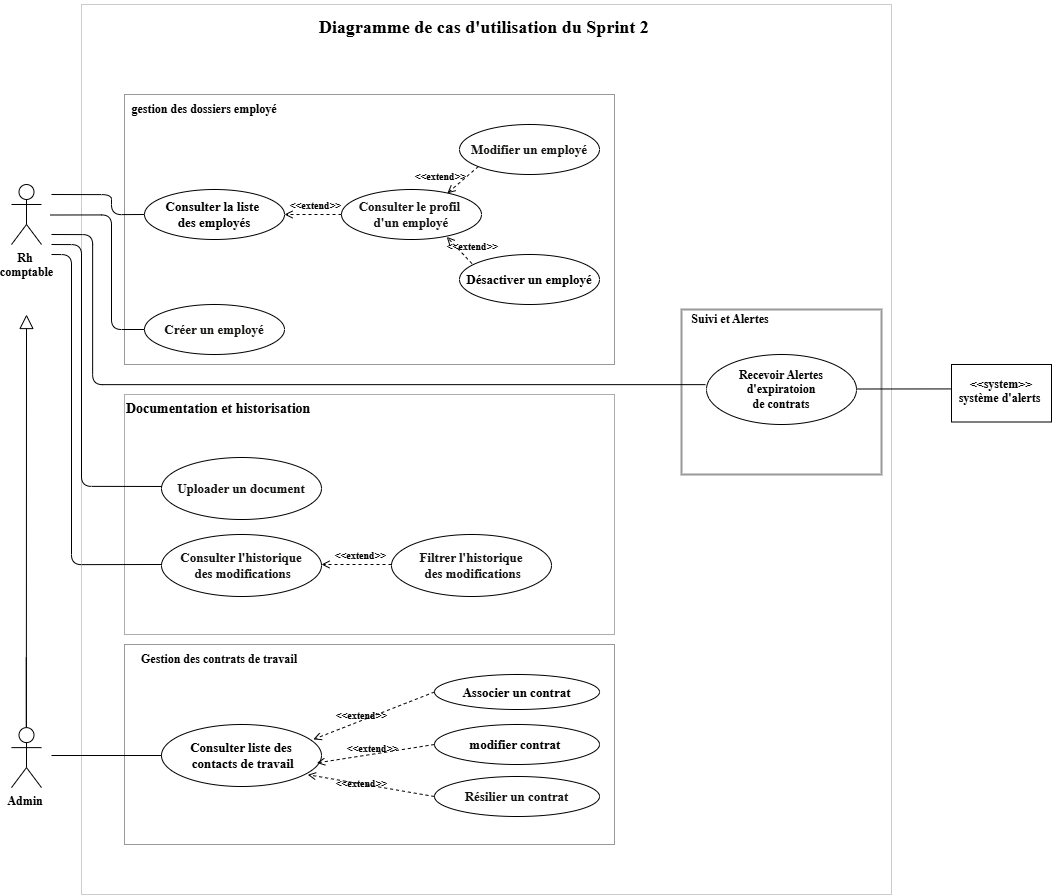
\includegraphics[width=0.95\textwidth]{use-case-sp2.png}
    \caption{Diagramme de cas d'utilisation du Sprint~2}
    \label{fig:use-case-sp2}
\end{figure}

Le diagramme de cas d'utilisation du Sprint~2 (Figure~\ref{fig:uc-sprint2})
  organise les fonctionnalités en trois packages fonctionnels distincts,
  reflétant les trois domaines couverts~: gestion du capital humain,
  gestion des contrats et gestion documentaire.

  \textbf{Relations UML~:} Le cas d'utilisation \og{}Consulter le profil
  employé\fg{} est en relation \texttt{<<include>>} avec
  \og{}Gérer les contrats\fg{} et \og{}Gérer les documents\fg{}, car le
  profil constitue le point d'entrée unique vers ces sous-modules. La
  relation de généralisation \textsc{Admin}~$\rightarrow$~\textsc{RH}
  héritée du Sprint~1 reste active~: l'Admin dispose de l'ensemble des
  droits du RH.

  \textbf{Responsabilités par acteur~:}

  \begin{itemize}
    \item \textbf{Admin Entreprise~:}
          Dispose de tous les droits du RH par héritage~; peut en sus
          superviser l'ensemble du personnel sans restriction de département.

    \item \textbf{RH Comptable~:}
          \begin{itemize}
            \item Gérer l'intégralité du dossier employé (créer, consulter,
                  modifier, désactiver).
            \item Associer, modifier et résilier les contrats de travail
                  (CDI, CDD, CIVP, KARAMA, Intérimaire, Stage).
            \item Déposer et consulter les documents administratifs
                  (\texttt{HrDocument}) dans le dossier employé.
            \item Consulter l'historique des modifications
                  (\texttt{EmployeeHistory}) pour tout dossier employé.
          \end{itemize}
  \end{itemize}

% -----------------------------------------------------------
\subsection{Description textuelle des cas d'utilisation}
% -----------------------------------------------------------

Les descriptions textuelles suivantes formalisent les préconditions,
scénarios nominaux et alternatifs des cas d'utilisation les plus
critiques du Sprint~2. Elles constituent la référence contractuelle de
validation avec le Product Owner.

% -----------------------------------------------------------
\subsubsection{Cas d'utilisation 1 : Créer un employé}
% -----------------------------------------------------------

Le tableau~\ref{tab:uc_creer_employe} présente la description textuelle
détaillée du cas d'utilisation «~Créer un employé~».
% ── CU 1 : Créer un employé ───────────────────────────────
\vspace{0.2cm}
\begin{xltabular}{\textwidth}{|l|X|}
    \hline
    \rowcolor[gray]{0.9} \textbf{Élément} & \textbf{Description} \\ \hline
    \endfirsthead
    \hline
    \rowcolor[gray]{0.9} \textbf{Élément} & \textbf{Description} \\ \hline
    \endhead
    \hline
    \endfoot
    \endlastfoot

    \textbf{Titre} & Créer un employé \\ \hline
    \textbf{Acteur principal} & Admin / RH Comptable \\ \hline
    \textbf{Préconditions} & L'utilisateur est authentifié (rôle Admin ou RH).
        Au moins un département et un poste actifs existent dans le système. \\ \hline
    \textbf{Postconditions} & Un nouveau profil employé est enregistré avec un
        matricule unique auto-généré. L'employé apparaît dans la liste du personnel
        de la société. L'action est tracée dans le journal d'audit. \\ \hline
    \textbf{Scénario principal} &
    \begin{enumerate}[nosep, leftmargin=*]
        \item L'acteur accède au formulaire de création d'un employé.
        \item Il renseigne les informations d'identité~: nom, prénom
              (en français et en arabe), date et lieu de naissance,
              genre, nationalité, numéro CIN, numéro CNSS.
        \item Il renseigne les informations fiscales et sociales~:
              situation familiale (\texttt{maritalStatus}), nombre
              d'enfants à charge (\texttt{numberOfChildren}), statut
              de chef de famille (\texttt{chefDeFamille}) ---
              ces données conditionnent le calcul de l'IRPP.
        \item Il renseigne les informations de contact~: adresse,
              ville, e-mail professionnel, téléphone, RIB bancaire.
        \item Il sélectionne le département, le poste et la catégorie
              de l'employé.
        \item Il renseigne la date d'embauche et la date de fin de
              période d'essai (optionnelle).
        \item Le système valide toutes les données saisies.
        \item Le système génère un matricule unique (format~: préfixe
              société + séquence auto-incrémentée).
        \item Le profil est enregistré en base et un message de
              confirmation est affiché.
    \end{enumerate} \\ \hline
    \textbf{Scénarios alternatifs}
    & \textbf{A1~: Données obligatoires manquantes} $\rightarrow$
      Erreurs de validation affichées sur les champs concernés~;
      la création est bloquée. \\ \cline{2-2}
    & \textbf{A2~: CIN déjà enregistré} $\rightarrow$
      Le système affiche un message d'unicité~; la création est bloquée. \\ \cline{2-2}
    & \textbf{A3~: Département ou poste inactif} $\rightarrow$
      Message d'erreur indiquant que la structure organisationnelle
      sélectionnée est inactive. \\ \hline
    \caption{Description textuelle du CU~: Créer un employé}
    \label{tab:uc_creer_employe}
\end{xltabular}
% -----------------------------------------------------------
\subsubsection{Cas d'utilisation 2 : Gérer les contrats de travail}
% -----------------------------------------------------------

Le tableau~\ref{tab:uc_gestion_contrats} présente la description
textuelle détaillée du cas d'utilisation «~Gérer les contrats de
travail~».
% ── CU 2 : Gérer les contrats de travail ─────────────────
\vspace{0.2cm}
\begin{xltabular}{\textwidth}{|l|X|}
    \hline
    \rowcolor[gray]{0.9} \textbf{Élément} & \textbf{Description} \\ \hline
    \endfirsthead
    \hline
    \rowcolor[gray]{0.9} \textbf{Élément} & \textbf{Description} \\ \hline
    \endhead
    \hline
    \endfoot
    \endlastfoot

    \textbf{Titre} & Gérer les contrats de travail
        (Associer / Modifier / Résilier) \\ \hline
    \textbf{Acteur principal} & RH Comptable \\ \hline
    \textbf{Préconditions} & L'utilisateur est authentifié (rôle RH).
        L'employé cible est actif dans le système et ne possède pas de
        contrat actif (pour une association). \\ \hline
    \textbf{Postconditions} & Le contrat est créé, modifié ou résilié.
        L'action est enregistrée dans le journal d'audit. \\ \hline
    \textbf{Scénario principal} &
    \begin{enumerate}[nosep, leftmargin=*]
        \item Le RH accède au profil de l'employé, onglet «~Contrats~».
        \item Il sélectionne l'action souhaitée~: association,
              modification ou résiliation.
        \item \textbf{Association~:} il sélectionne le type de contrat
              parmi les six types tunisiens supportés~:
              \textbf{CDI}, \textbf{CDD},
              \textbf{CIVP}, \textbf{KARAMA}, \textbf{Intérimaire} ou \textbf{Stage}~;
              il renseigne les conditions (date de début, salaire brut
              de base, heures hebdomadaires, convention collective)
              et confirme.
        \item \textbf{Modification~:} il met à jour les champs autorisés
              sur le contrat actif (hors type et date de début) et confirme.
        \item \textbf{Résiliation~:} il renseigne le motif de résiliation
              (champ obligatoire) et la date effective, puis confirme.
        \item Le système valide, applique les changements, met à jour
              le statut (ACTIF ~$\rightarrow$~ RÉSILIÉ)
              et enregistre l'action en base.
        \item Un message de confirmation est affiché.
    \end{enumerate} \\ \hline
    \textbf{Scénarios alternatifs}
    & \textbf{A1~: Contrat actif déjà existant} $\rightarrow$
      Le système bloque la création et affiche un message d'erreur. \\ \cline{2-2}
    & \textbf{A2~: Date de fin antérieure à la date de début (CDD)}
      $\rightarrow$ Erreur de validation bloquante. \\ \cline{2-2}
    & \textbf{A3~: Motif de résiliation absent} $\rightarrow$
      Erreur de validation~; le champ est obligatoire. \\ \cline{2-2}
    & \textbf{A4~: Durée CIVP dépassant 12~mois} $\rightarrow$
      Le système alerte que ce type de contrat est limité à un an. \\ \hline
    \caption{Description textuelle du CU~: Gérer les contrats de travail}
    \label{tab:uc_gestion_contrats}
\end{xltabular}
% -----------------------------------------------------------
\subsubsection{Cas d'utilisation 3 : Déposer un document administratif}
% -----------------------------------------------------------

Le tableau~\ref{tab:uc_deposer_document} présente la description
textuelle détaillée du cas d'utilisation «~Déposer un document
administratif~».
% ── CU 3 : Déposer un document administratif ─────────────
\vspace{0.2cm}
\begin{xltabular}{\textwidth}{|l|X|}
    \hline
    \rowcolor[gray]{0.9} \textbf{Élément} & \textbf{Description} \\ \hline
    \endfirsthead
    \hline
    \rowcolor[gray]{0.9} \textbf{Élément} & \textbf{Description} \\ \hline
    \endhead
    \hline
    \endfoot
    \endlastfoot

    \textbf{Titre} & Déposer un document administratif \\ \hline
    \textbf{Acteur principal} & RH \\ \hline
    \textbf{Préconditions} & L'utilisateur est authentifié avec le rôle RH.
        L'employé cible est enregistré dans le système. \\ \hline
    \textbf{Postconditions} & Le document est stocké et associé au dossier
        de l'employé. Le dépôt est tracé automatiquement dans le journal
        d'audit. \\ \hline
    \textbf{Scénario principal} &
    \begin{enumerate}[nosep, leftmargin=*]
        \item Le RH accède au profil de l'employé, section «~Documents~».
        \item Il clique sur «~Ajouter un document~».
        \item Il sélectionne le type de document (CONTRAT, ATTESTATION,
              DIPLOME, AUTRE).
        \item Il joint le fichier à déposer.
        \item Le système valide le format et la taille du fichier.
        \item Le document est enregistré avec ses métadonnées
              (type, auteur, horodatage).
        \item Un message de confirmation est affiché.
    \end{enumerate} \\ \hline
    \textbf{Scénarios alternatifs}
    & \textbf{A1~: Format de fichier non supporté} $\rightarrow$
      Un message d'erreur liste les formats acceptés~;
      le dépôt est bloqué. \\ \cline{2-2}
    & \textbf{A2~: Taille du fichier dépassant la limite autorisée}
      $\rightarrow$ Un message d'erreur indique la taille maximale
      autorisée~; le dépôt est bloqué. \\ \hline
    \caption{Description textuelle du CU~: Déposer un document administratif}
    \label{tab:uc_deposer_document}
\end{xltabular}

% ============================================================
\section{Conception du deuxième Sprint}
\label{sec:s2-conception}
% ============================================================

La conception technique du Sprint~2 traduit les besoins métiers en
modèles structurants guidant le développement. Cette section s'articule
autour de deux axes complémentaires~: le diagramme de classes, qui
modélise l'architecture statique des nouvelles entités, et les
diagrammes de séquence, qui illustrent les interactions dynamiques entre
les composants du système.

% -----------------------------------------------------------
\subsection{Diagramme de classes}
% -----------------------------------------------------------

Le diagramme de classes du Sprint~2 étend le modèle établi lors du
Sprint~1 en introduisant les nouvelles entités du domaine RH. Il définit
la structure des données --- employés, contrats et documents
--- ainsi que les relations de dépendance qui les unissent avec les
entités existantes (UserProfile, Company, Department,JobPosition).

La figure~\ref{fig:classes-sprint2} présente le diagramme de classes du
Sprint~2, illustrant l'extension du modèle de données.

\begin{figure}[H]
    \centering
    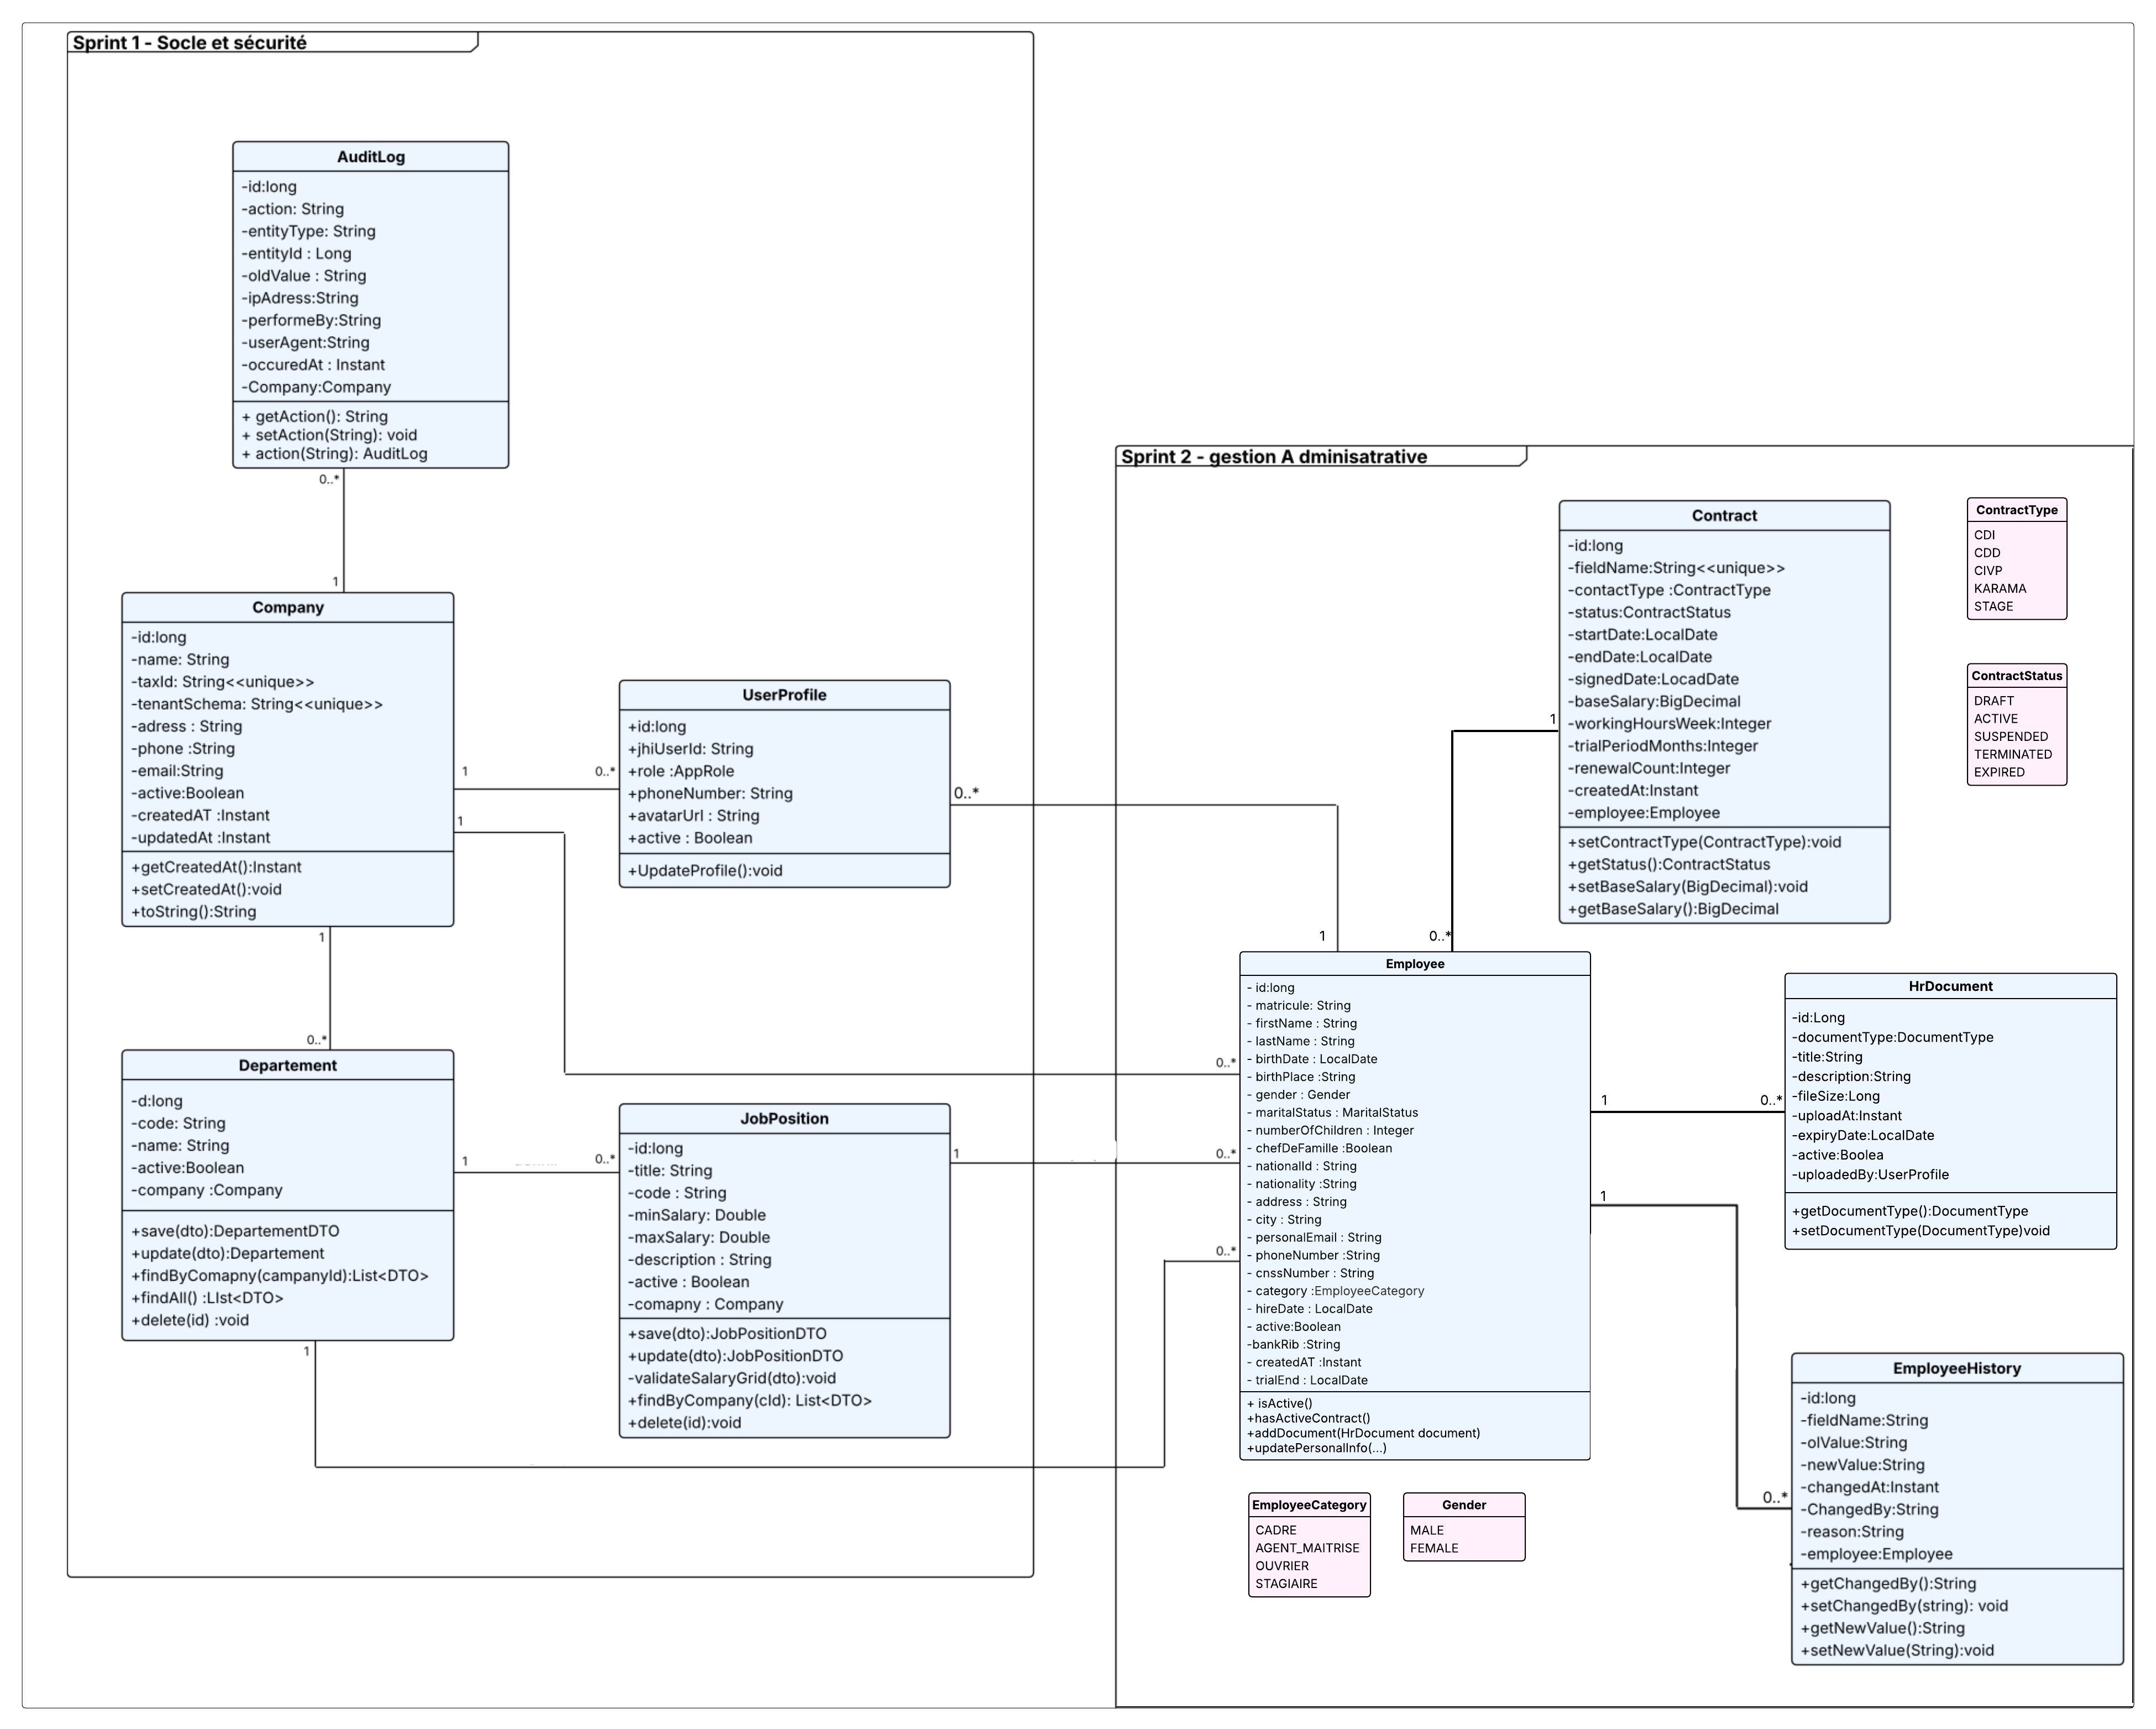
\includegraphics[width=1\textwidth]{classes-sprint2}
    \caption{Diagramme de classes du Sprint~2}
    \label{fig:classes-sprint2}
\end{figure}

Les entités principales introduites dans ce sprint sont les suivantes~:

\begin{itemize}
    \item \textbf{Employee}~: entité centrale du sprint.
          Outre les informations d'identité (matricule, nom, prénom, CIN,
          date de naissance, genre, nationalité, numéro CNSS), elle stocke
          les données fiscales et sociales indispensables au moteur de paie
          du Sprint~3~: la situation familiale, le nombre d'enfants à charge,
          le statut de chef de famille (déductible IRPP), le RIB bancaire
          pour virement et le solde de congés. Elle est associée à la société,
          au département et au poste, et peut être liée au compte
          d'authentification de l'utilisateur. Une auto-association
          optionnelle modélise la relation hiérarchique entre un employé
          et son responsable.

    \item \textbf{Contract}~: représente le contrat de travail d'un employé.
          Elle porte une référence unique, le type de contrat (CDI, CDD,
          CIVP, KARAMA, Intérimaire, Stage), le statut (actif, résilié
          ou suspendu), les dates clés (début et fin), le salaire brut
          de base, la durée hebdomadaire de travail, la convention
          collective applicable et la durée de la période d'essai.

    \item \textbf{HrDocument}~: modélise les pièces administratives attachées
          au dossier d'un employé (CV, diplômes, scans de contrats,
          attestations manuelles). Elle est identifiée par son type
          (contrat, attestation, diplôme ou autre), son titre et les
          métadonnées de dépôt (auteur, horodatage, taille).
\end{itemize}
% -----------------------------------------------------------
\subsection{Diagrammes de séquences}
% -----------------------------------------------------------

Les diagrammes de séquences illustrent la dynamique du système en
détaillant les interactions chronologiques entre les composants pour
les cas d'utilisation les plus critiques.

\subsubsection{Diagramme de séquence : Création d'un employé}

La figure~\ref{fig:seq-create-employe} illustre le flux de création
d'un employé dans PaieZone, incluant la génération du matricule et le
déclenchement automatique de l'enregistrement dans l'historique.

\begin{figure}[H]
    \centering
    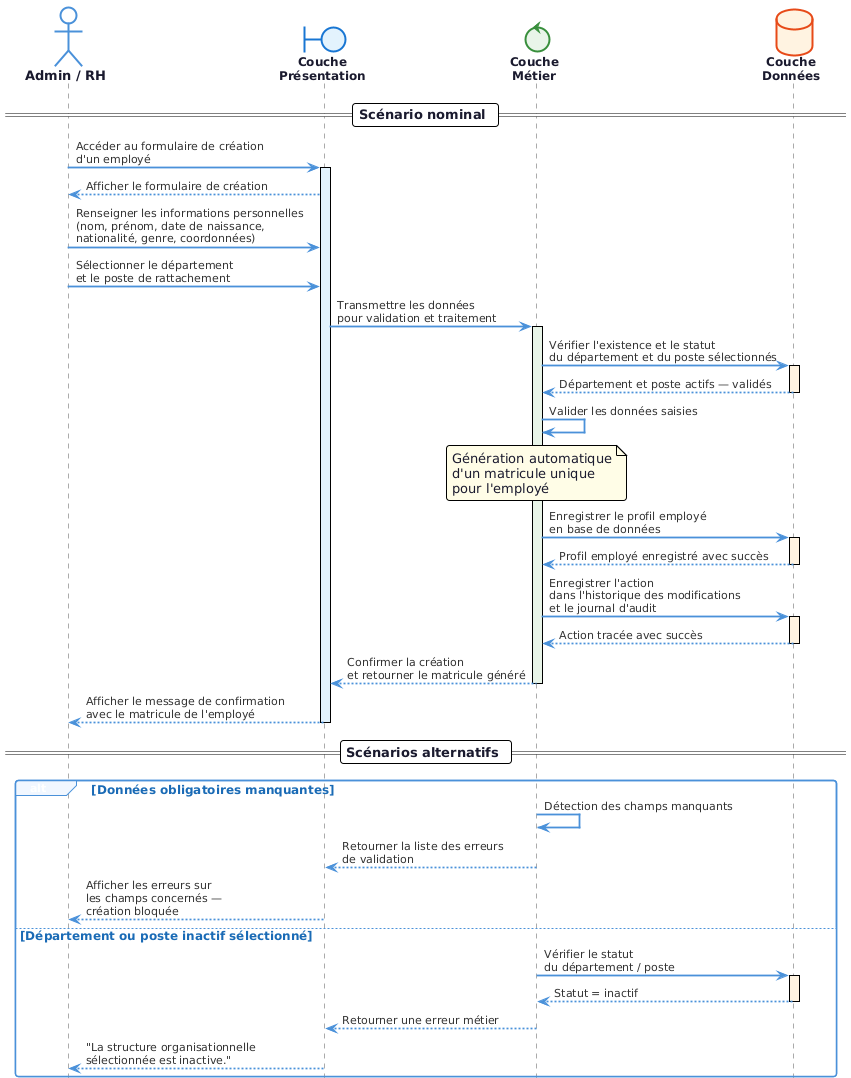
\includegraphics[width=0.91\textwidth]{seq-sp2-uc1.png}
    \caption{Diagramme de séquence --- Création d'un employé}
    \label{fig:seq-create-employe}
\end{figure}
\subsubsection{Diagramme de séquence : Association d'un contrat}

La figure~\ref{fig:seq-create-contrat} illustre le flux d'association
d'un contrat de travail à un employé dans PaieZone, incluant les
validations métier et la mise à jour du statut.

\begin{figure}[H]
    \centering
    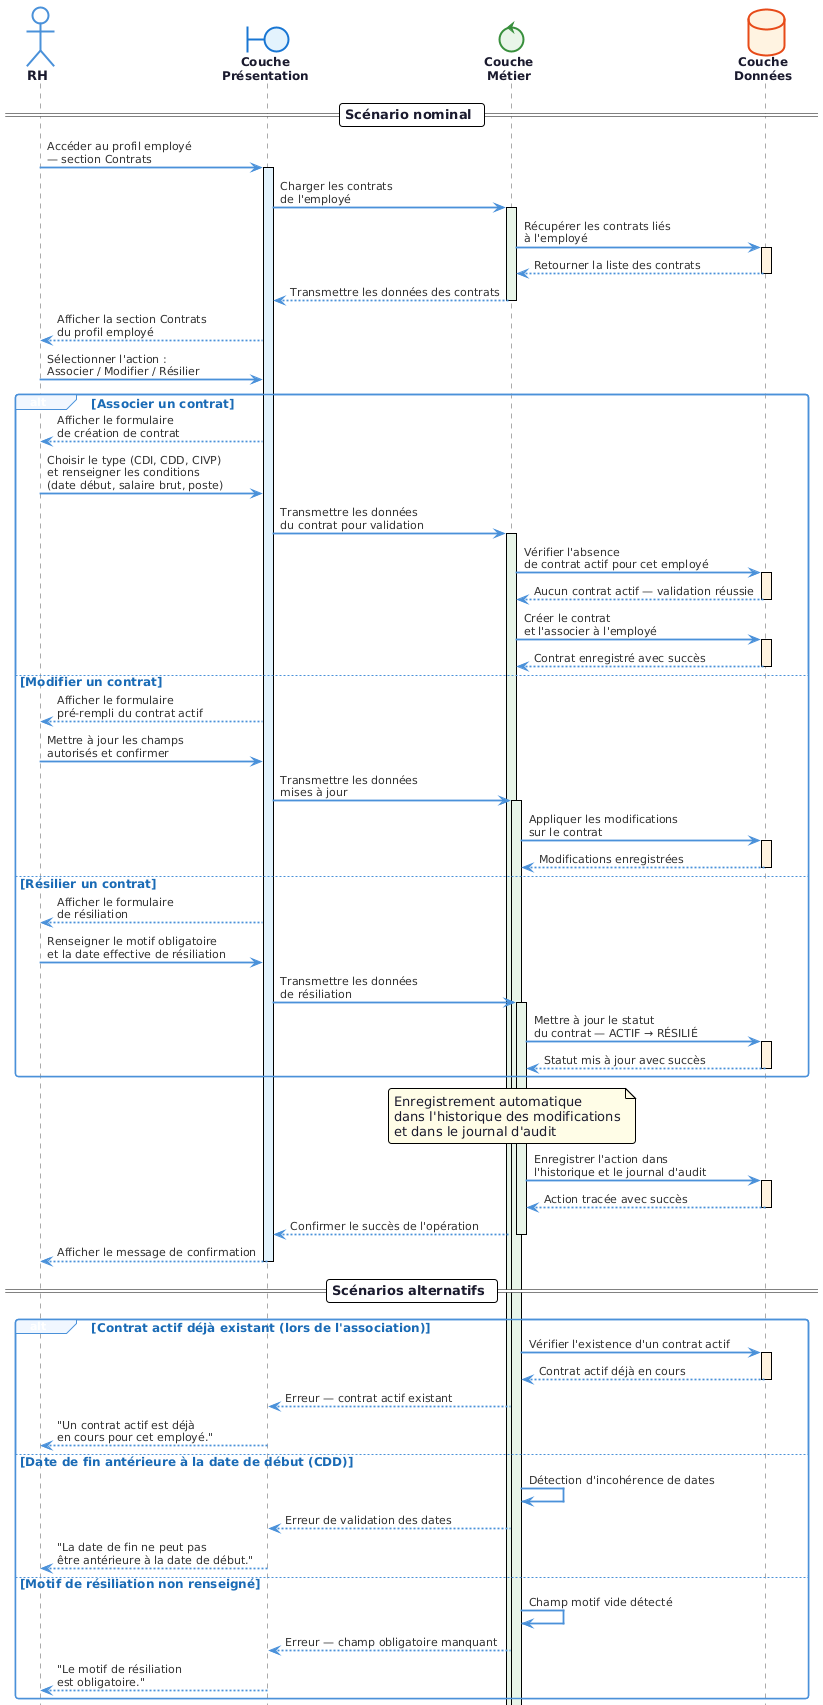
\includegraphics[width=0.69\textwidth]{seq-sp2-uc2.png}
    \caption{Diagramme de séquence --- Association d'un contrat à un
             employé}
    \label{fig:seq-create-contrat}
\end{figure}



% ============================================================
\section{Étude et réalisation du deuxième sprint}
\label{sec:s2-realisation}
% ============================================================

Cette section présente les réalisations concrètes du Sprint~2, marquant
le passage des spécifications à des fonctionnalités opérationnelles
livrées. Les travaux ont porté sur l'implémentation du module de gestion
des employés, le cycle de vie des contrats de travail, la gestion
documentaire et le système d'historisation. Ces développements
matérialisent la validation des 10 User Stories planifiées et
constituent le c\oe{}ur métier RH de la plateforme PaieZone.

% -----------------------------------------------------------
\subsection{Gestion des employés}
% -----------------------------------------------------------

Le module de gestion des employés constitue l'épine dorsale du
Sprint~2. Il offre à l'équipe RH et aux Administrateurs un contrôle
complet sur les dossiers du personnel de la société.

\begin{figure}[H]
    \centering
    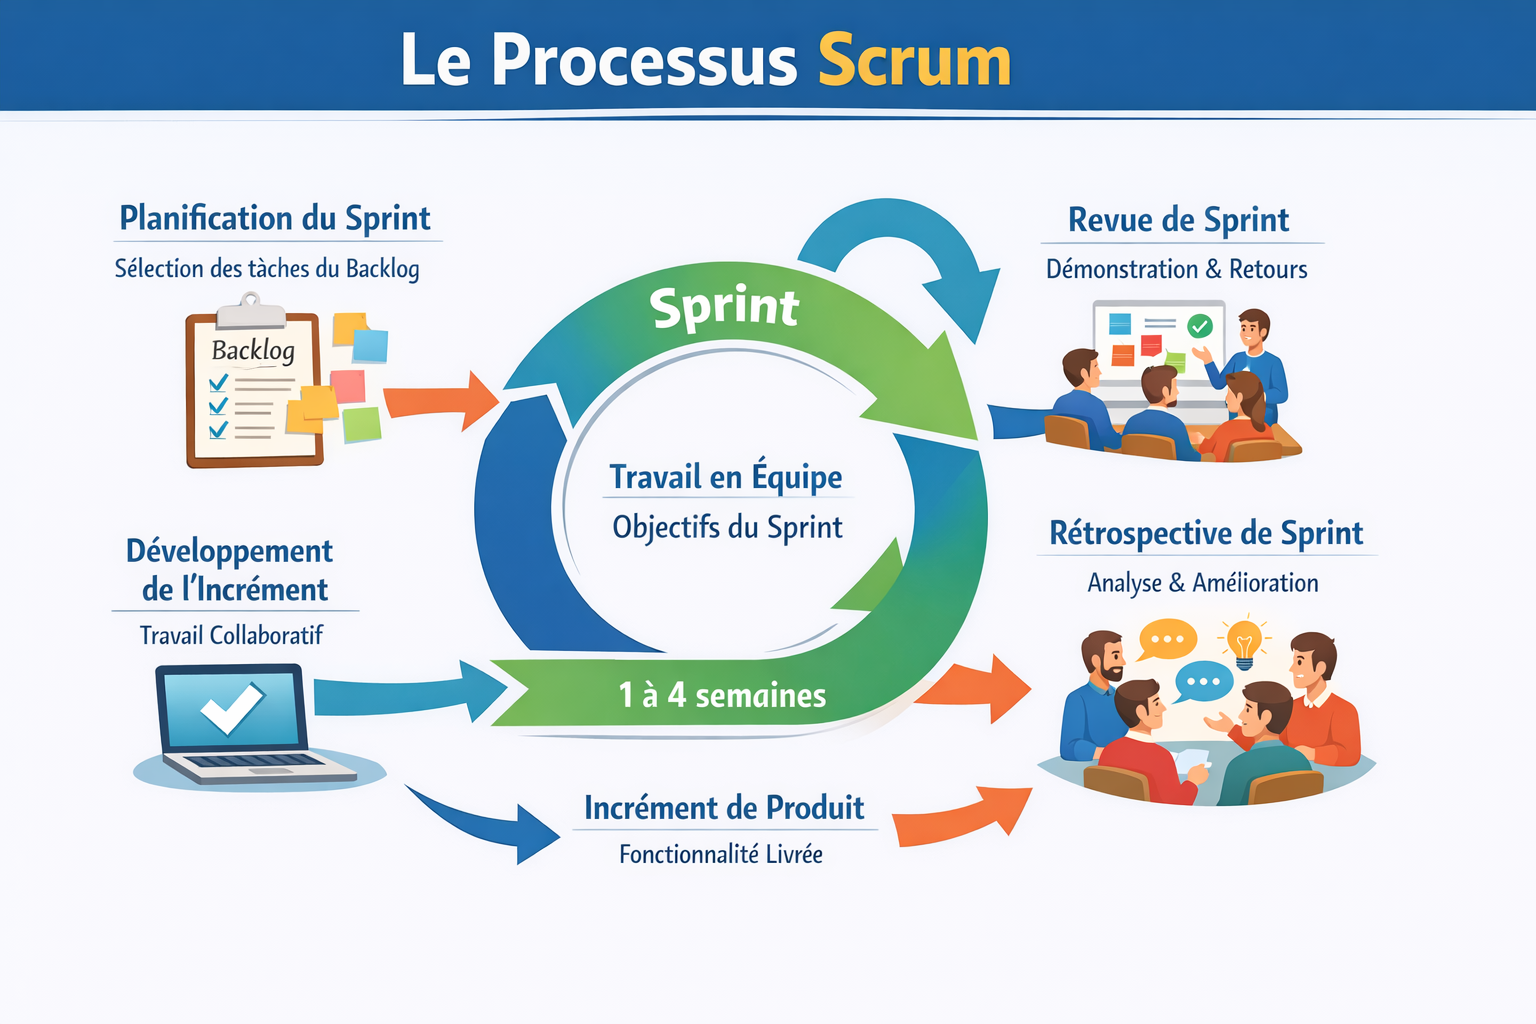
\includegraphics[width=0.70\textwidth]{scrum.png}
    \caption{Liste des employés --- Vue d'ensemble du personnel}
    \label{fig:ui-employees-list}
\end{figure}

La figure~\ref{fig:ui-employees-list} illustre l'interface de
consultation de la liste des employés. Les collaborateurs sont présentés
avec leurs informations clés~: matricule, identité, département, poste
et statut. La table intègre des fonctions de recherche multicritère et
de pagination pour faciliter la navigation au sein des effectifs.

\newpage

\begin{figure}[H]
    \centering
    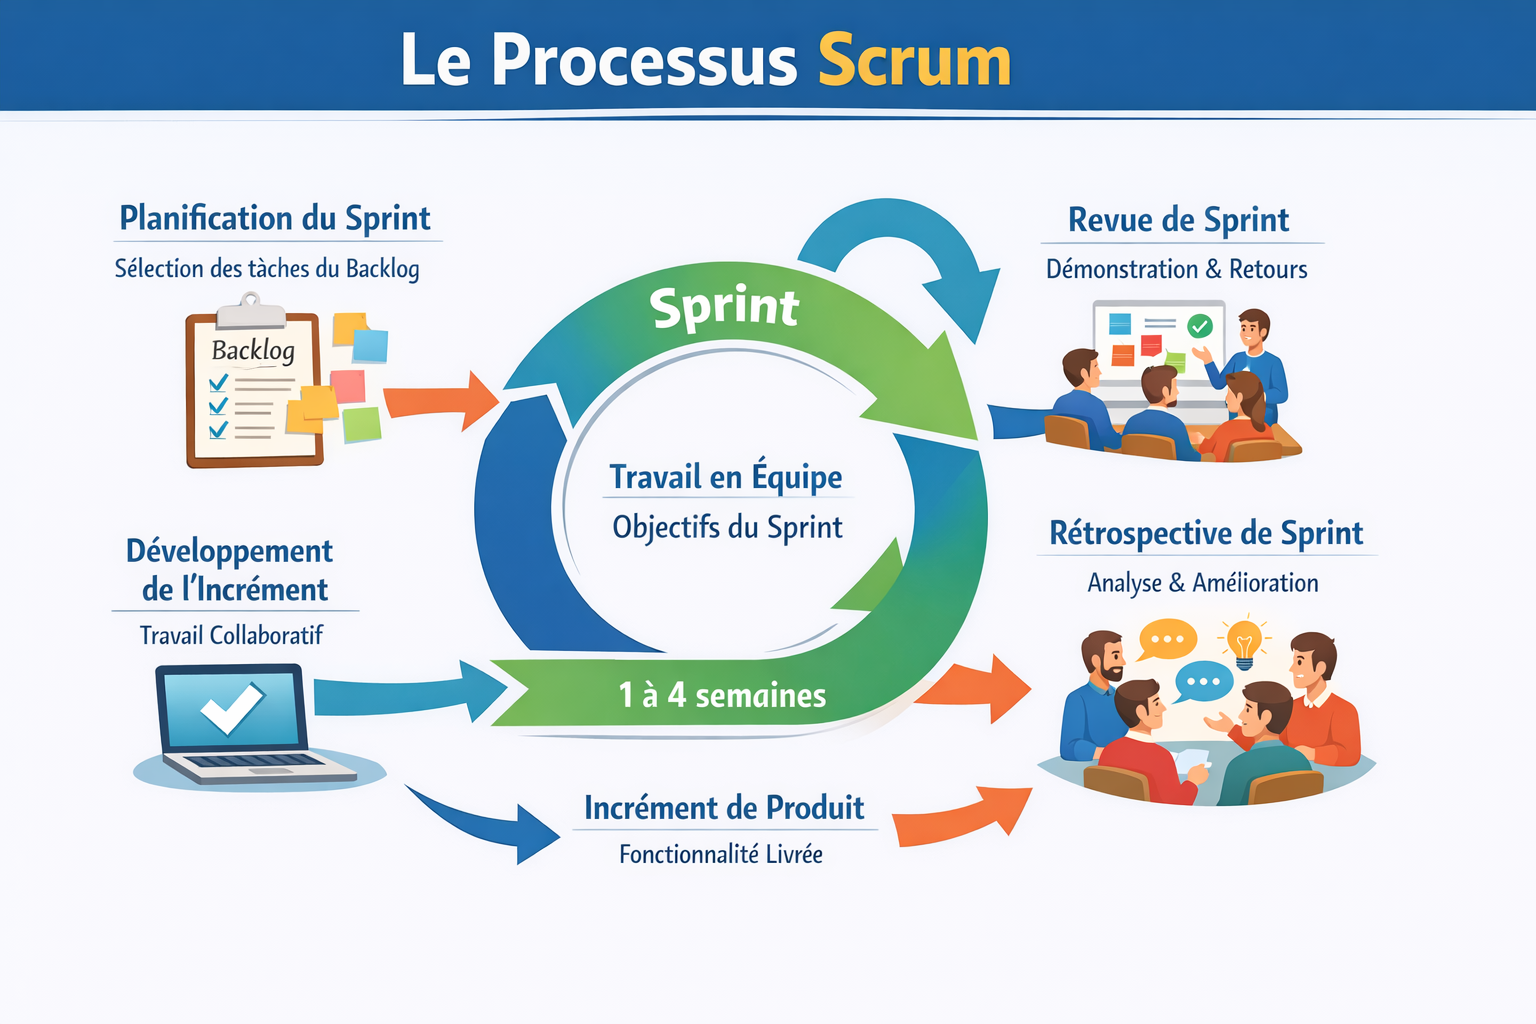
\includegraphics[width=0.70\textwidth]{scrum.png}
    \caption{Formulaire de création et de modification d'un employé}
    \label{fig:ui-employee-form}
\end{figure}

La Figure~\ref{fig:ui-employee-form} présente l'interface dédiée à la gestion 
des dossiers employés. Ce formulaire permet de renseigner l'ensemble des informations personnelles, fiscales et administratives nécessaires au suivi du collaborateur. Pour garantir la fiabilité du système, chaque saisie fait l'objet d'un contrôle automatique rigoureux, empêchant ainsi les erreurs de format ou la création de profils en double.

\begin{figure}[H]
    \centering
    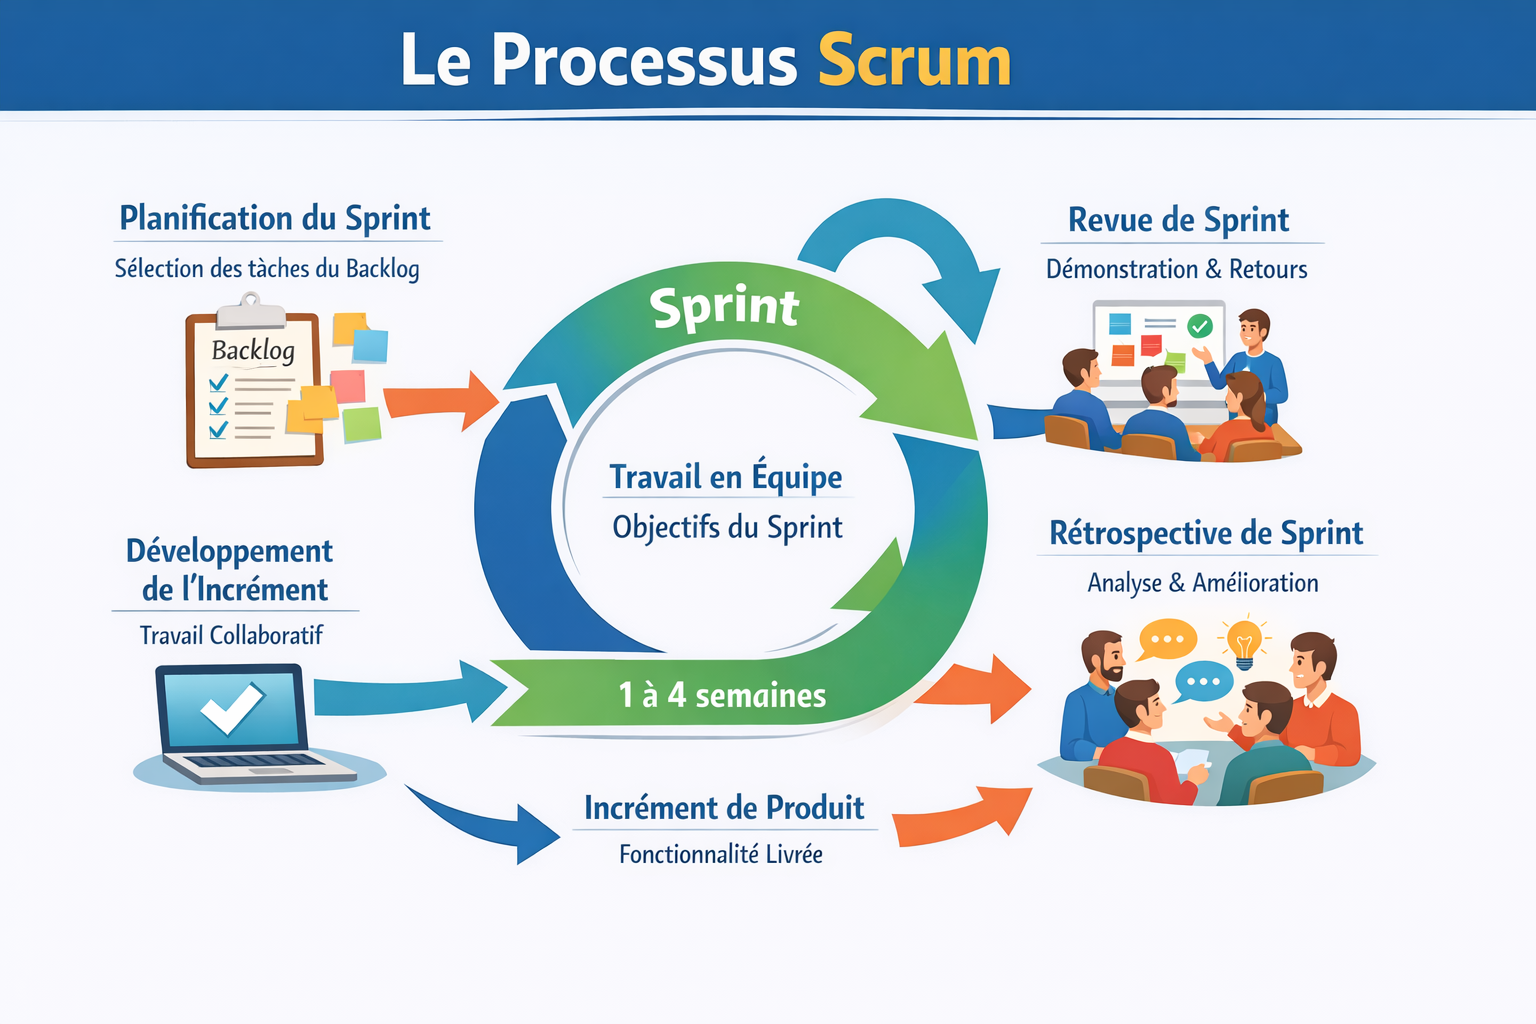
\includegraphics[width=0.70\textwidth]{scrum.png}
    \caption{Vue détaillée du profil employé}
    \label{fig:ui-employee-profile}
\end{figure}

La figure~\ref{fig:ui-employee-profile} illustre la vue détaillée du
profil d'un employé, centralisant l'ensemble de son dossier
administratif~: informations personnelles, contrats associés, documents
stockés et historique des modifications. Cette vue constitue le point
d'entrée unique pour toutes les opérations liées au dossier d'un
collaborateur.

% -----------------------------------------------------------
\subsection{Gestion des contrats de travail}
% -----------------------------------------------------------

Le module de gestion des contrats formalise la relation de travail entre
l'employé et la société. Il couvre l'intégralité du cycle de vie
contractuel~: association, modification et résiliation.

\begin{figure}[H]
    \centering
    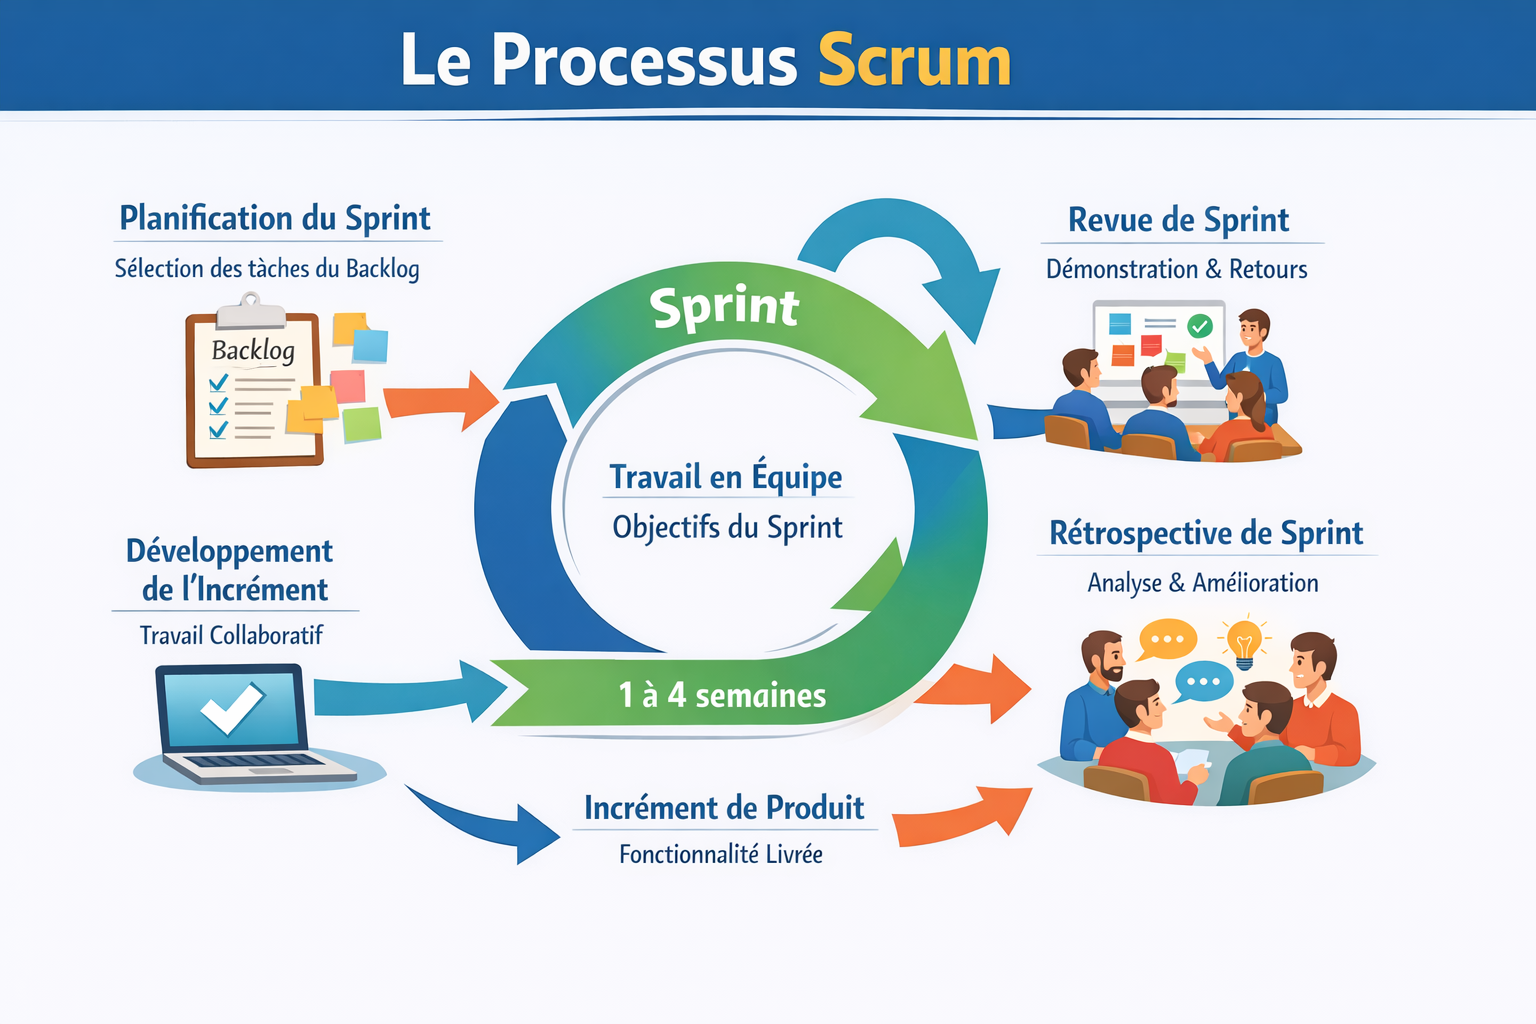
\includegraphics[width=0.70\textwidth]{scrum.png}
    \caption{Section Contrats du dossier employé}
    \label{fig:ui-contracts-list}
\end{figure}

La figure~\ref{fig:ui-contracts-list} présente la section «~Contrats~»
du dossier employé, affichant l'historique contractuel avec le type, le
statut, les dates clés et le salaire brut. Les actions disponibles
(modifier, résilier) sont conditionnées au statut courant du contrat,
empêchant toute opération incohérente.

% -----------------------------------------------------------
\subsection{Gestion des documents administratifs}
% -----------------------------------------------------------

Le module de gestion documentaire permet à l'équipe RH de constituer un
dossier numérique complet pour chaque employé, en stockant de manière
sécurisée l'ensemble des pièces administratives.
\newpage

\begin{figure}[H]
    \centering
    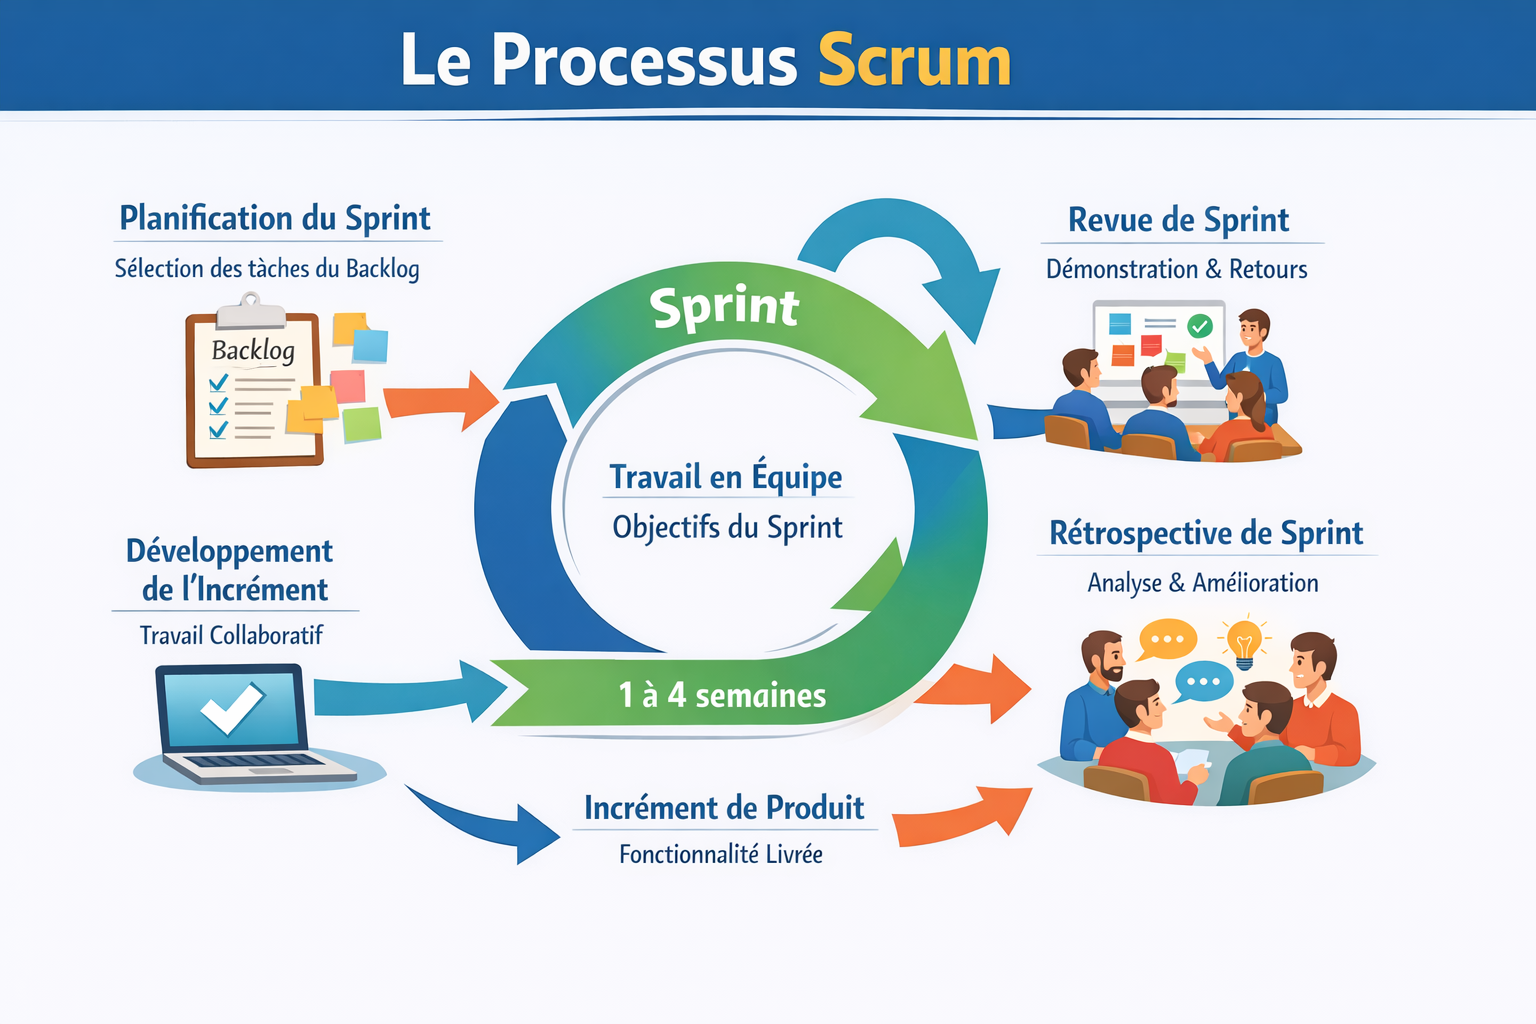
\includegraphics[width=0.70\textwidth]{scrum.png}
    \caption{Section Documents du dossier employé --- Dépôt et
             consultation}
    \label{fig:ui-documents}
\end{figure}

La figure~\ref{fig:ui-documents} présente la section «~Documents~» du
dossier employé. Le RH peut déposer des fichiers en sélectionnant leur
type parmi une liste prédéfinie (CONTRAT, ATTESTATION, DIPLOME, AUTRE).
Chaque document est référencé avec son nom, son type et la date de dépôt.


% ============================================================
\section{Tests et Validation}
\label{sec:s2-tests}
% ============================================================

La phase de tests et de validation du Sprint~2 vise à garantir la
conformité des fonctionnalités implémentées aux exigences des User
Stories et à assurer la robustesse des modules métier livrés. Trois
niveaux de tests ont été mis en œuvre de manière complémentaire.

% -----------------------------------------------------------
\subsection{Plan de tests}
% -----------------------------------------------------------

\begin{itemize}[label=\textbullet, leftmargin=0.6cm]
    \item \textbf{Tests unitaires :} Sécurisent les règles de gestion internes (statuts des contrats, formats documentaires).
    \item \textbf{Tests d'intégration:} Confirment l'interopérabilité entre les différents modules (employés, postes, contrats).
    \item \textbf{Tests fonctionnels:} Valident l'ergonomie des formulaires et la fiabilité des affichages dynamiques sous Angular.
\end{itemize}
Cette démarche rigoureuse assure que chaque fonctionnalité développée est strictement conforme aux critères d'acceptation des User Stories. Le Tableau~\ref{tab:tests-sprint2} récapitule les principaux scénarios de test exécutés, confirmant ainsi la stabilité et la validité du système pour ce sprint.
principaux réalisés pour ce sprint.
\renewcommand{\arraystretch}{1.3}
\begin{xltabular}{\textwidth}{|p{1.5cm}|X|p{4cm}|p{1.5cm}|}
\hline
\rowcolor[gray]{0.9}
\textbf{ID} & \textbf{Description} & \textbf{Résultat attendu} & \textbf{Statut} \\ \hline
\endfirsthead
\hline
\rowcolor[gray]{0.9}
\textbf{ID} & \textbf{Description} & \textbf{Résultat attendu} & \textbf{Statut} \\ \hline
\endhead
\hline
\endfoot
\hline
\caption{Récapitulatif des cas de test du Sprint~2}
\label{tab:tests-sprint2}
\endlastfoot

T-6.1 & Création d'un employé avec tous les champs valides
       & Employé créé avec matricule auto-généré, persisté en base
       & \textcolor{green!60!black}{\textbf{OK}} \\ \hline

T-6.2 & Création d'un employé avec CIN déjà existant
       & Erreur d'unicité, création bloquée
       & \textcolor{green!60!black}{\textbf{OK}} \\ \hline

T-6.3 & Désactivation d'un employé possédant un contrat actif
       & Avertissement affiché, désactivation conditionnelle
       & \textcolor{green!60!black}{\textbf{OK}} \\ \hline

T-7.1 & Association d'un contrat CDI à un employé sans contrat actif
       & Contrat créé avec statut ACTIF
       & \textcolor{green!60!black}{\textbf{OK}} \\ \hline

T-7.2 & Association d'un contrat CIVP avec une durée supérieure à 12~mois
       & Alerte de durée maximale affichée
       & \textcolor{green!60!black}{\textbf{OK}} \\ \hline

T-7.3 & Tentative d'association d'un second contrat actif sur un employé
        déjà sous contrat
       & Blocage avec message d'erreur explicite
       & \textcolor{green!60!black}{\textbf{OK}} \\ \hline

T-7.4 & Résiliation d'un contrat sans motif renseigné
       & Erreur de validation, résiliation bloquée
       & \textcolor{green!60!black}{\textbf{OK}} \\ \hline

T-8.1 & Dépôt d'un fichier PDF valide dans le dossier employé
       & Document enregistré et visible dans la liste des documents
       & \textcolor{green!60!black}{\textbf{OK}} \\ \hline

T-8.2 & Dépôt d'un fichier de format non supporté (ex.~: .exe)
       & Rejet avec message listant les formats acceptés
       & \textcolor{green!60!black}{\textbf{OK}} \\ \hline

\end{xltabular}
\renewcommand{\arraystretch}{1.0}

% -----------------------------------------------------------
\subsection{Tests automatisés}
% -----------------------------------------------------------

Pour le Sprint~2, les tests automatisés ont ciblé le flux d'approbation
des avances sur salaire --- l'un des processus métier à changements d'état
les plus sensibles de la plateforme.

\paragraph{Tests unitaires --- AdvanceWorkflowTest (JUnit~5 + Mockito)}
Quatre cas de test valident les transitions d'état du service \texttt{AdvanceServiceImpl}~:

\renewcommand{\arraystretch}{1.2}
\begin{small}
\begin{xltabular}{\textwidth}{|c|X|p{4cm}|c|}
\hline
\rowcolor[gray]{0.9}
\textbf{ID} & \textbf{Scénario} & \textbf{Résultat attendu} & \textbf{Statut} \\ \hline
\endfirsthead \hline
\rowcolor[gray]{0.9}
\textbf{ID} & \textbf{Scénario} & \textbf{Résultat attendu} & \textbf{Statut} \\ \hline
\endhead \hline \endfoot \hline
\caption{Tests automatisés --- AdvanceWorkflowTest}\label{tab:auto-s2}\endlastfoot
TA-S2-01 & Approbation d'une avance au statut \texttt{REQUESTED}
    & Statut passe à \texttt{APPROVED} & \textcolor{green!60!black}{\textbf{OK}} \\ \hline
TA-S2-02 & Refus d'une avance au statut \texttt{REQUESTED}
    & Statut passe à \texttt{REJECTED} & \textcolor{green!60!black}{\textbf{OK}} \\ \hline
TA-S2-03 & Approbation d'une avance déjà \texttt{APPROVED}
    & Exception levée (\textit{transition interdite}) & \textcolor{green!60!black}{\textbf{OK}} \\ \hline
TA-S2-04 & Avance introuvable en base
    & Exception \texttt{404 Not Found} & \textcolor{green!60!black}{\textbf{OK}} \\ \hline
\end{xltabular}
\end{small}
\renewcommand{\arraystretch}{1.0}

\textbf{Résultat~:} 4/4 tests passés (\textcolor{green!60!black}{\textbf{OK}}).

% ============================================================
\section{Rituels Agiles et Clôture du Sprint}
\label{sec:s2-rituels}
% ============================================================

Conformément à la méthodologie Scrum adoptée par l'équipe PaieZone,
le Sprint~2 s'est clôturé par la tenue des deux rituels essentiels~:
la Sprint Review et la Sprint Retrospective. Ces cérémonies assurent
la transparence du travail accompli et l'amélioration continue des
pratiques d'équipe.
% -----------------------------------------------------------
\subsection{Revue du Sprint (Sprint Review)}
% -----------------------------------------------------------

La Sprint Review a réuni l'équipe de développement, le Product Owner
et les parties prenantes. Les démonstrations ont couvert la gestion
du capital humain (création, modification et désactivation des profils
employés), l'association des six types de contrats tunisiens (CDI, CDD,
CIVP, KARAMA, Intérimaire et Stage), ainsi que le dépôt et la
consultation des documents administratifs. L'ensemble des 9 User
Stories planifiées a été validé par le Product Owner, confirmant la
conformité des livrables aux critères d'acceptation.
% -----------------------------------------------------------
\subsection{Rétrospective du Sprint (Sprint Retrospective)}
% -----------------------------------------------------------

La rétrospective a permis à l'équipe de réfléchir sur trois axes~:

\begin{itemize}[label=\textbullet, leftmargin=0.6cm]
    \item \textbf{Ce qui a bien fonctionné~:} La synergie entre les
          équipes front-end et back-end a garanti une livraison fluide
          des fonctionnalités. La réutilisation des composants Angular
          existants a accéléré le développement des interfaces de
          gestion des employés et des contrats.

    \item \textbf{Problèmes rencontrés~:} La gestion du stockage des
          fichiers (formats, tailles, types) a engendré des contraintes
          techniques imprévues, nécessitant des ajustements de la
          configuration du service de stockage en cours de sprint.

    \item \textbf{Actions d'amélioration pour le Sprint~3~:} Anticiper
          l'analyse des dépendances techniques entre les modules dès
          le début du sprint afin de réduire les blocages en cours de
          développement et de garantir une livraison dans les délais
          prévus.
\end{itemize}
\section*{Conclusion}
\label{sec:s2-conclusion}
\addcontentsline{toc}{section}{Conclusion}

Ce chapitre a détaillé la mise en œuvre du cœur métier RH de PaieZone RH. La validation des User Stories liées à la gestion des employés, des contrats tunisiens et de la GED (Gestion Électronique des Documents) a permis de consolider le référentiel de données avec les entités clés.

Ces acquis constituent le socle indispensable pour le Sprint 3 : les paramètres fiscaux et sociaux ainsi que les conditions contractuelles seront directement exploités par le moteur de calcul.

Le chapitre suivant sera consacré au Sprint 3, portant sur l'automatisation de la paie, les déclarations sociales et la gestion des absences.



% ==========================================
% CHAPITRE 5 — ÉTUDE DU SPRINT 3
% Corrigé selon rapport de jury
% ==========================================
\newpage
\chapter{ÉTUDE DU SPRINT 3}

\noindent \textbf{\Large Plan}
\vspace{0.8cm}

\begin{enumerate}[label=\textbf{\arabic*}, leftmargin=1.5cm, labelsep=0.8cm]
    \item[] \hspace*{-1.5cm}\textbf{Introduction}                        \dotfill \pageref{sec:s3-intro}
    \item \textbf{User Stories du troisième sprint}                       \dotfill \pageref{sec:s3-userstories}
    \item \textbf{Backlog du troisième Sprint}                            \dotfill \pageref{sec:s3-backlog}
    \item \textbf{Spécification fonctionnelle}                            \dotfill \pageref{sec:s3-specification}
    \item \textbf{Conception du Sprint 3}                                 \dotfill \pageref{sec:s3-conception}
    \item \textbf{Étude et réalisation}                                   \dotfill \pageref{sec:s3-realisation}
    \item \textbf{Tests et Validation}                                    \dotfill \pageref{sec:s3-tests}
    \item \textbf{Rituels Agiles et Clôture du Sprint}                    \dotfill \pageref{sec:s3-rituels}
    \item[] \hspace*{-1.5cm}\textbf{Conclusion}                          \dotfill \pageref{sec:s3-conclusion}
\end{enumerate}
\vfill
\newpage

% ============================================================
\section*{Introduction}
\label{sec:s3-intro}
\addcontentsline{toc}{section}{Introduction}
% ============================================================

S'appuyant sur le référentiel de données consolidé lors des phases
précédentes, ce chapitre présente les réalisations du Sprint~3, qui
constitue le c\oe{}ur métier différenciant de la plateforme PaieZone~RH.
Cette itération est dédiée à l'automatisation de la paie et à la gestion
du temps, intégrant le paramétrage réglementaire tunisien, le calcul des
bulletins de paie, les déclarations sociales (CNSS) ainsi que le suivi
des congés et des absences.

Le présent chapitre suit la structure agile standard des chapitres
précédents~: spécification via les User Stories et le Sprint Backlog,
modélisation UML (cas d'utilisation, classes, séquences), réalisation
des interfaces Angular, validation par plan de tests multiniveaux,
puis clôture agile (Sprint Review et Rétrospective).

% ============================================================
\section{User Stories du troisième sprint}
\label{sec:s3-userstories}
% ============================================================

Le tableau~\ref{tab:us-sprint3} présente les vingt-deux User Stories
identifiées pour le Sprint~3 de PaieZone, réparties sur trois domaines
fonctionnels~: la gestion des paramètres réglementaires, la gestion
de la paie et la gestion des congés et des absences.

\begin{small}
\renewcommand{\arraystretch}{1.4}
\begin{longtable}{|>{\bfseries}p{1.2cm}|p{9.5cm}|>{\centering\arraybackslash}p{2.5cm}|}
\hline
\rowcolor[gray]{0.9} \textbf{ID} & \textbf{User Story} & \textbf{Priorité} \\ \hline
\endfirsthead
\hline
\rowcolor[gray]{0.9} \textbf{ID} & \textbf{User Story} & \textbf{Priorité} \\ \hline
\endhead
\hline
\endfoot
\hline
\caption{User Stories du Sprint 3 }
\label{tab:us-sprint3}
\endlastfoot

10.1 & En tant que Super Admin, je souhaite \textbf{consulter la liste des paramètres réglementaires} afin de vérifier les taux légaux en vigueur. & Haute \\ \hline
10.2 & En tant que Super Admin, je souhaite \textbf{ajouter un nouveau paramètre réglementaire} afin d'intégrer une nouvelle règle légale dans le système. & Haute \\ \hline
10.3 & En tant que Super Admin, je souhaite \textbf{modifier un paramètre réglementaire} afin de mettre à jour les taux conformément aux évolutions législatives. & Haute \\ \hline
10.4 & En tant que Super Admin, je souhaite \textbf{consulter l'historique des modifications des paramètres} afin de garantir la traçabilité des changements réglementaires. & Moyenne \\ \hline
11.1 & En tant que RH, je souhaite \textbf{créer une période de paie} afin de lancer le cycle de traitement des salaires. & Critique \\ \hline
11.2 & En tant que RH, je souhaite \textbf{modifier une période de paie} afin de corriger les données avant la clôture. & Haute \\ \hline
11.3 & En tant que RH, je souhaite \textbf{clôturer une période de paie} afin de valider les calculs et de bloquer toute modification ultérieure. & Critique \\ \hline
11.4 & En tant que RH, je souhaite \textbf{lancer le calcul de tous les bulletins d'une période} afin de générer automatiquement les salaires nets de l'ensemble du personnel. & Critique \\ \hline
11.5 & En tant que RH, je souhaite \textbf{créer une rubrique de paie} afin de structurer les éléments de calcul du salaire. & Haute \\ \hline
11.6 & En tant que RH, je souhaite \textbf{modifier une rubrique de paie} afin de l'adapter aux besoins de la société. & Moyenne \\ \hline
11.7 & En tant que RH, je souhaite \textbf{ajouter une prime} à un employé afin d'augmenter sa rémunération pour une période donnée. & Haute \\ \hline
11.8 & En tant que RH, je souhaite \textbf{modifier une prime} afin d'ajuster son montant avant le calcul de la paie. & Moyenne \\ \hline
11.9 & En tant que RH, je souhaite \textbf{valider une demande d'avance} afin d'accorder le soutien financier sollicité par l'employé. & Haute \\ \hline
11.10 & En tant que RH, je souhaite \textbf{refuser une demande d'avance} afin d'informer l'employé du rejet de sa demande. & Haute \\ \hline
11.11 & En tant qu'Employé, je souhaite \textbf{demander une avance sur salaire} afin de recevoir un soutien financier ponctuel. & Haute \\ \hline
11.12 & En tant que RH, je souhaite \textbf{générer un bulletin de paie} afin de le distribuer à l'employé concerné. & Critique \\ \hline
11.13 & En tant que RH, je souhaite \textbf{générer un fichier CNSS} afin de déclarer les salariés auprès de la Caisse Nationale de Sécurité Sociale. & Critique \\ \hline
12.1 & En tant que RH, je souhaite \textbf{créer un type de congé} afin de définir les règles et les quotas associés. & Haute \\ \hline
12.2 & En tant qu'Employé, je souhaite \textbf{demander un congé} afin de m'absenter légitimement de mon poste de travail. & Haute \\ \hline
12.3 & En tant que RH, je souhaite \textbf{valider une demande de congé} afin de gérer la disponibilité et la continuité du service. & Haute \\ \hline
12.4 & En tant qu'Employé, je souhaite \textbf{consulter mon solde de congé} afin de planifier mes absences en connaissance de cause. & Haute \\ \hline
12.5 & En tant que RH, je souhaite \textbf{gérer les jours fériés} afin de les intégrer automatiquement dans le calcul de la paie et dans la gestion des congés. & Moyenne \\

\end{longtable}
\end{small}
\renewcommand{\arraystretch}{1.0}

% ============================================================
\section{Backlog du troisième Sprint}
\label{sec:s3-backlog}
% ============================================================

Le Tableau~\ref{tab:backlog-sprint3} détaille le backlog complet du
troisième Sprint, regroupant la gestion des paramètres réglementaires,
le traitement de la paie, ainsi que le suivi des congés et des absences.

\begin{small}
\renewcommand{\arraystretch}{1.4}
\begin{longtable}{|>{\raggedright\arraybackslash}p{2.8cm}|>{\raggedright\arraybackslash}p{6.2cm}|>{\raggedright\arraybackslash}p{6.2cm}|c|}

\hline
\rowcolor[gray]{0.9} \textbf{Item} & \textbf{User Story} & \textbf{Tâches} & \makecell{\textbf{Est.}\\\textbf{(j)}} \\ \hline
\endfirsthead
\hline
\rowcolor[gray]{0.9} \textbf{Item} & \textbf{User Story} & \textbf{Tâches} & \makecell{\textbf{Est.}\\\textbf{(j)}} \\ \hline
\endhead
\hline
\endfoot
\hline
\caption{Backlog détaillé du troisième Sprint}
\label{tab:backlog-sprint3} 
\endlastfoot

\multirow{4}{*}{\makecell[c]{\textbf{Gestion des}\\ \textbf{Paramètres}\\ \textbf{Réglementaires}}}
& \textbf{10.1} En tant que Super Admin, je souhaite consulter la liste des paramètres réglementaires afin de vérifier les taux légaux en vigueur.
& - Concevoir l'interface de consultation des paramètres réglementaires.\newline
- Développer l'API REST de récupération des paramètres actifs.
& \textbf{1} \\ \cline{2-4}

& \textbf{10.2} En tant que Super Admin, je souhaite ajouter un nouveau paramètre réglementaire afin d'intégrer une nouvelle règle légale.
& - Développer le formulaire d'ajout d'un paramètre (taux, date d'entrée en vigueur).\newline
- Implémenter l'API REST d'insertion avec versionnage.\newline
- Tester la prise en compte du nouveau taux dans les calculs de paie.
& \textbf{1} \\ \cline{2-4}

& \textbf{10.3} En tant que Super Admin, je souhaite modifier un paramètre réglementaire afin de mettre à jour les taux conformément aux évolutions législatives.
& - Développer l'interface de modification du paramètre.\newline
- Implémenter la traçabilité des modifications dans le journal d'audit.\newline
- Tester l'impact de la mise à jour sur les calculs historiques.
& \textbf{1} \\ \cline{2-4}

& \textbf{10.4} En tant que Super Admin, je souhaite consulter l'historique des modifications des paramètres afin de garantir la traçabilité des changements réglementaires.
& - Créer l'interface de consultation de l'historique des paramètres.\newline
- Développer l'API REST de récupération des versions antérieures.
& \textbf{1} \\ \hline

\multirow{3}{*}{\makecell[c]{\textbf{Gestion des}\\ \textbf{Périodes}\\ \textbf{de Paie}}}
& \textbf{11.1} En tant que RH, je souhaite créer une période de paie afin de lancer le cycle de traitement des salaires.
& - Concevoir l'interface de création d'une période de paie (mois, année).\newline
- Développer l'API REST de création de la période.\newline
- Tester les contraintes de dates et l'unicité de la période.
& \textbf{1} \\ \cline{2-4}

& \textbf{11.2} En tant que RH, je souhaite modifier une période de paie afin de corriger les données avant la clôture.
& - Développer l'interface de modification de la période.\newline
- Implémenter les contrôles de modification (période non clôturée uniquement).\newline
- Tester les transitions de statut.
& \textbf{1} \\ \cline{2-4}

& \textbf{11.3} En tant que RH, je souhaite clôturer une période de paie afin de valider les calculs et de bloquer toute modification ultérieure.
& - Implémenter le verrouillage de la période et de tous ses bulletins.\newline
- Développer l'API REST de clôture avec horodatage .\newline
- Tester le blocage effectif des modifications post-clôture.
& \textbf{1} \\ \hline

\multirow{1}{*}{\makecell[c]{\textbf{Calcul des}\\ \textbf{Bulletins}\\ \textbf{de Paie}}}
& \textbf{11.4} En tant que RH, je souhaite lancer le calcul de tous les bulletins d'une période afin de générer automatiquement les salaires nets de l'ensemble du personnel.
& - Implémenter le moteur de calcul du salaire net (rubriques, cotisations CNSS/CAVIS/CSS, IRPP, primes, avances).\newline
- Implémenter le traitement en lot.\newline

- Intégrer les paramètres réglementaires dans le moteur de calcul.\newline
- Tester les cas limites (prime, avance, mi-temps).
& \textbf{5} \\ \hline

\multirow{4}{*}{\makecell[c]{\textbf{Rubriques}\\ \textbf{\& Primes}}}
& \textbf{11.5} En tant que RH, je souhaite créer une rubrique de paie afin de structurer les éléments de calcul du salaire.
& - Concevoir l'interface de création d'une rubrique (type, montant, nature : gain/retenue).\newline
- Développer l'API REST d'insertion de la rubrique.\newline
- Tester la prise en compte de la rubrique dans le calcul du bulletin.
& \textbf{1} \\ \cline{2-4}

& \textbf{11.6} En tant que RH, je souhaite modifier une rubrique de paie afin de l'adapter aux besoins de la société.
& - Développer l'interface de modification de la rubrique.\newline
- Implémenter la mise à jour en base avec contrôle de cohérence.
& \textbf{1} \\ \cline{2-4}

& \textbf{11.7} En tant que RH, je souhaite ajouter une prime à un employé afin d'augmenter sa rémunération pour une période donnée.
& - Développer l'interface et l'API REST de création d'une prime individuelle.\newline
- Tester l'intégration de la prime dans le calcul du bulletin.
& \textbf{1} \\ \cline{2-4}

& \textbf{11.8} En tant que RH, je souhaite modifier une prime afin d'ajuster son montant avant le calcul de la paie.
& - Développer l'interface de modification de la prime.\newline
- Implémenter la mise à jour avec contrôle du statut de la période.
& \textbf{1} \\ \hline

\multirow{3}{*}{\makecell[c]{\textbf{Gestion}\\ \textbf{des Avances}}}
& \textbf{11.9} En tant que RH, je souhaite valider une demande d'avance afin d'accorder le soutien financier sollicité par l'employé.
& - Implémenter le workflow de validation par le RH.\newline
- Mettre à jour le statut en "APPROVED".\newline
- Tester la déduction automatique de l'avance dans le bulletin.
& \textbf{1} \\ \cline{2-4}

& \textbf{11.10} En tant que RH, je souhaite refuser une demande d'avance afin d'informer l'employé du rejet.
& - Implémenter le workflow de refus avec saisie obligatoire d'une raison.\newline
- Mettre à jour le statut en "REJECTED".\newline
- Tester la notification de refus à l'employé.
& \textbf{1} \\ \cline{2-4}

& \textbf{11.11} En tant qu'Employé, je souhaite demander une avance sur salaire afin de recevoir un soutien financier ponctuel.
& - Développer l'interface de demande d'avance (formulaire employé : montant, raison).\newline
- Implémenter les contrôles (contrat actif, plafond autorisé).\newline
- Tester le cycle complet de la demande à la déduction.
& \textbf{1} \\ \hline

\multirow{2}{*}{\makecell[c]{\textbf{Génération}\\ \textbf{des Documents}\\ \textbf{de Paie}}}
& \textbf{11.12} En tant que RH, je souhaite générer un bulletin de paie afin de le distribuer à l'employé concerné.
& - Concevoir et implémenter le template PDF du bulletin de paie.\newline
- Développer le service de génération PDF.\newline
- Implémenter la mise à disposition du bulletin dans l'espace employé.\newline
- Tester la conformité du PDF avec les paramètres réglementaires.
& \textbf{2} \\ \cline{2-4}

& \textbf{11.13} En tant que RH, je souhaite générer un fichier CNSS afin de déclarer les salariés auprès de la Caisse Nationale de Sécurité Sociale.
& - Développer le service de génération du fichier CNSS au format réglementaire.\newline
- Agréger les montants CNSS salarié et patronal par employé.\newline
- Tester la conformité du fichier généré avec les exigences légales.
& \textbf{2} \\ \hline

\multirow{5}{*}{\makecell[c]{\textbf{Gestion des}\\ \textbf{Congés \&}\\ \textbf{Absences}}}
& \textbf{12.1} En tant que RH, je souhaite créer un type de congé afin de définir les règles et les quotas associés.
& - Concevoir l'interface de création d'un type de congé (annuel, maladie, sans solde).\newline
- Développer l'API REST d'insertion avec gestion des quotas.
& \textbf{1} \\ \cline{2-4}

& \textbf{12.2} En tant qu'Employé, je souhaite demander un congé afin de m'absenter légitimement de mon poste de travail.
& - Développer l'interface de demande de congé (formulaire, calendrier).\newline
- Implémenter les contrôles de solde et de chevauchement.\newline
- Tester la création de la demande avec le statut \texttt{PENDING}.
& \textbf{1} \\ \cline{2-4}

& \textbf{12.3} En tant que RH, je souhaite valider une demande de congé afin de gérer la disponibilité et la continuité du service.
& - Implémenter le workflow de validation/refus par le RH avec notification.\newline
- Mettre à jour automatiquement le solde après approbation.\newline
- Tester la décrémentation du solde.
& \textbf{1} \\ \cline{2-4}

& \textbf{12.4} En tant qu'Employé, je souhaite consulter mon solde de congé afin de planifier mes absences en connaissance de cause.
& - Développer l'interface de consultation du solde de congé par type.\newline
- Développer l'API REST de récupération du solde en temps réel.
& \textbf{1} \\ \cline{2-4}

& \textbf{12.5} En tant que RH, je souhaite gérer les jours fériés afin de les intégrer automatiquement dans le calcul de la paie et dans la gestion des congés.
& - Implémenter la gestion des jours fériés (ajout, suppression).\newline
- Intégrer l'exclusion automatique des jours fériés dans le décompte des congés.\newline
- Tester la prise en compte des jours fériés dans le calcul de paie.
& \textbf{1} \\ \hline

\end{longtable}
\end{small}
\renewcommand{\arraystretch}{1.0}
\normalsize

% ============================================================
\section{Spécification fonctionnelle}
\label{sec:s3-specification}
% ============================================================

La spécification fonctionnelle du Sprint~3 formalise les besoins
exprimés par le Product Owner autour des trois épopées majeures de
ce sprint. Les exigences déjà recueillies dans les User Stories et
le Backlog sont ici modélisées par les diagrammes UML correspondants
et leurs descriptions textuelles contractuelles.

% -----------------------------------------------------------
\subsection{Diagramme de cas d'utilisation du Sprint 3}
% -----------------------------------------------------------

\begin{figure}[H]
  \centering
  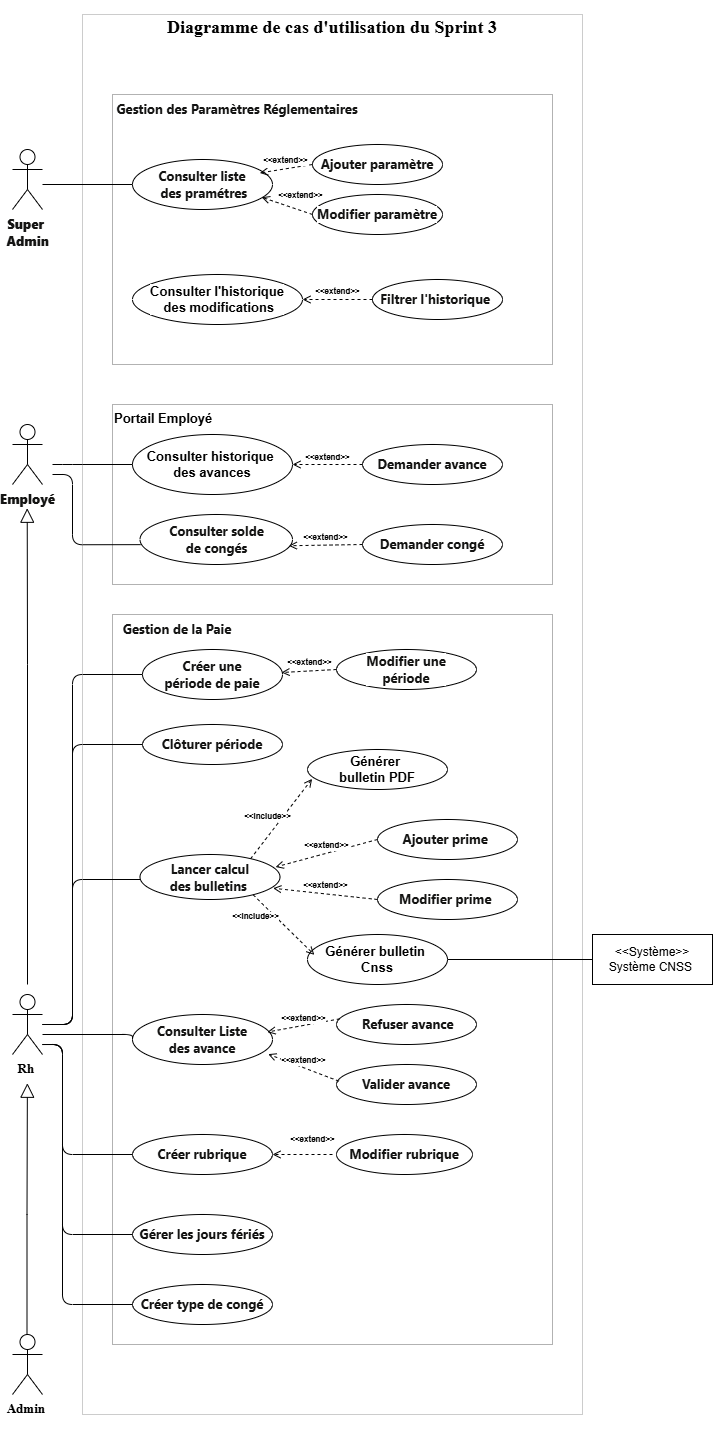
\includegraphics[width=0.69\textwidth]{use-case-sp3.png}
  \caption{Diagramme de cas d'utilisation du Sprint~3}
  \label{fig:uc-sprint3}
\end{figure}

Le diagramme de cas d'utilisation du Sprint~3 organise les fonctionnalités
en trois packages distincts, chacun associé à des acteurs définis~:

\begin{itemize}[label=\textbullet, leftmargin=0.6cm]
    \item \textbf{Gestion des paramètres réglementaires~:}
          Réservé exclusivement au Super Admin, 
          ce module gère les constantes légales configurables 
          sans redéploiement : le taux CNSS salarié, le taux CNSS
           patronal, le taux CAVIS, la CSS, la TFP, le barème IRPP
            progressif (Loi de Finances), et le SMIG. Chaque modification
             est versionnée et tracée dans le journal d’audit.

    \item \textbf{Gestion de la paie~:}
          Le RH Comptable pilote l'intégralité du cycle~:
          création et gestion des périodes de paie, configuration des
          rubriques et des éléments variables (primes, rubriques gain/
          retenue), lancement du calcul en lot, génération des bulletins
          PDF et du fichier de déclaration CNSS.
          L'Employé dispose d'un accès limité pour soumettre
          ses demandes d'avance sur salaire.

    \item \textbf{Gestion des congés et des absences~:}
          Le RH Comptable administre les types de congés
          (annuel, maladie, sans solde) et les jours fériés, et valide
          ou refuse les demandes soumises. L'Employé peut
          soumettre une demande de congé et consulter son solde en temps réel.
\end{itemize}

% -----------------------------------------------------------
\subsection{Description textuelle des cas d'utilisation}
% -----------------------------------------------------------

Les descriptions textuelles suivantes formalisent les scénarios des
cas d'utilisation principaux du Sprint~3. Elles constituent la
référence contractuelle de validation avec le Product Owner lors de
la Sprint Review.
\subsubsection{Cas d'utilisation 1 : Lancer le calcul de tous les bulletins d'une période}

Le tableau~\ref{tab:cu-calcul} présente la description textuelle détaillée
du cas d'utilisation « Lancer le calcul des bulletins de paie ».
\mbox{}\\

\begin{xltabular}{\textwidth}{|l|X|}
\hline
\rowcolor[gray]{0.9} \textbf{Élément} & \textbf{Description} \\ \hline
\endfirsthead
\hline
\caption{Description textuelle du CU~: Lancer le calcul des bulletins de paie}
\label{tab:cu-calcul} 
\endlastfoot
\textbf{Titre} & Lancer le calcul de tous les bulletins d'une période \\ \hline
\textbf{Acteur principal} & RH Comptable \\ \hline
\textbf{Préconditions} & Une période de paie existe au statut OUVERTE
  (non clôturée). Des employés actifs sont rattachés à la société.
  Les paramètres réglementaires (taux CNSS, barème IRPP, CSS) sont
  configurés par le Super Admin. \\ \hline
\textbf{Postconditions} & Tous les bulletins  sont générés
  au statut CALCULÉ. La période de paie passe au statut
 CALCULÉE. \\ \hline
\textbf{Scénario principal} &
    \begin{enumerate}[nosep, leftmargin=*]
        \item Le RH accède au module de paie et sélectionne une période en cours.
        \item Il clique sur « Lancer le calcul ».
        \item Le système vérifie que la période est modifiable.
        \item Le système récupère les données de rémunération, de temps de travail et d'absences de chaque employé.
        \item Le système calcule automatiquement les cotisations, les impôts et le salaire net.
        \item Le système génère et enregistre les bulletins de paie de tous les employés.
        \item Le système met à jour le statut de la période.
        \item Le système affiche un résumé global de l'opération au RH.
    \end{enumerate} 
 \\\hline
\textbf{Scénarios alternatifs}
& \textbf{A1~: Période clôturée}~$\rightarrow$ Le système bloque l'action et informe le RH. \\ \cline{2-2}
& \textbf{A2~: Aucun employé actif}~$\rightarrow$ Avertissement affiché, aucun bulletin créé. \\ \cline{2-2}
& \textbf{A3~: Paramètres réglementaires manquants}~$\rightarrow$ Erreur bloquante invitant le Super Admin à configurer les taux. \\
\end{xltabular}

\subsubsection{Cas d'utilisation 2 : Clôturer une période de paie}
Le tableau~\ref{tab:cu-cloture} présente la description textuelle détaillée
du cas d'utilisation « Clôturer une période de paie ».
\mbox{}\\
\begin{xltabular}{\textwidth}{|l|X|}

\hline
\rowcolor[gray]{0.9} \textbf{Élément} & \textbf{Description} \\ \hline
\endfirsthead
\hline
\caption{Description textuelle du CU~: Clôturer une période de paie}
\label{tab:cu-cloture}
\endlastfoot
\textbf{Titre} & Clôturer une période de paie \\ \hline
\textbf{Acteur principal} & RH \\ \hline
\textbf{Préconditions} & La période est au statut CALCULÉE. Tous les bulletins sont calculés. \\ \hline
\textbf{Postconditions} & La période passe au statut CLÔTURÉE . Aucune modification n'est possible. \\ \hline
\textbf{Scénario principal} &
\begin{enumerate}[nosep, leftmargin=*]
    \item Le RH accède à la liste des périodes de paie et sélectionne une période au statut CALCULÉE.
    \item Il clique sur « Clôturer la période ».
    \item Le système vérifie que tous les bulletins associés sont au statut CALCULÉ.
    \item Il verrouille tous les bulletins (CLÔTURÉ) et la période .
    \item Un message de confirmation s'affiche.
\end{enumerate} \\ \hline
\textbf{Scénarios alternatifs}
& \textbf{A1~: Bulletins non finalisés}~$\rightarrow$ Des bulletins sont encore en statut non calculé, le système bloque l'action avec un message d'erreur. \\ \cline{2-2}
& \textbf{A2~: Période déjà clôturée}~$\rightarrow$ Le système affiche un message informatif. \\
\end{xltabular}

\subsubsection{Cas d'utilisation 3 : Demande et traitement d'une avance sur salaire}

Le tableau~\ref{tab:cu-avance} présente la description textuelle détaillée
du cas d'utilisation « Demande et traitement d'une avance sur salaire ».
\mbox{}\\
\begin{xltabular}{\textwidth}{|l|X|}

\hline
\rowcolor[gray]{0.9} \textbf{Élément} & \textbf{Description} \\ \hline
\endfirsthead
\hline
\caption{Description textuelle du CU~: Demande et traitement d'une avance sur salaire}
\label{tab:cu-avance} 
\endlastfoot
\textbf{Titre} & Demande et traitement d'une avance sur salaire \\ \hline
\textbf{Acteurs principaux} & Employé (demandeur) --- RH Comptable (valideur) \\ \hline
\textbf{Préconditions} & L'employé possède un contrat actif. La période de paie est OUVERTE. Aucune avance en statut PENDING n'est en cours. \\ \hline
\textbf{Postconditions} & L'avance est au statut APPROVED et sera déduite du prochain bulletin, ou au statut REJECTED avec une raison enregistrée. \\ \hline
\textbf{Scénario principal} &
\begin{enumerate}[nosep, leftmargin=*]
    \item L'employé accède au module « Mes demandes d'avance ».
    \item Il renseigne le montant, la raison et la date de demande.
    \item Le système vérifie le contrat actif et le plafond autorisé.
    \item L'avance est créée avec le statut PENDING.
    \item Le RH consulte la liste des demandes en attente.
    \item Il sélectionne une demande et clique sur « Approuver ».
    \item Le système met à jour le statut $\rightarrow$ APPROVED.
    \item L'avance sera marquée DEDUCTED lors du calcul du bulletin.
\end{enumerate} \\ \hline
\textbf{Scénarios alternatifs}
& \textbf{A1~: Refus par le RH}~$\rightarrow$ Le RH saisit une raison et clique sur « Refuser », le système passe le statut à REJECTED. \\ \cline{2-2}
& \textbf{A2~: Montant invalide}~$\rightarrow$ Le montant dépasse le plafond autorisé, le système bloque la validation à la soumission. \\
\end{xltabular}

% ============================================================
\section{Conception du Sprint 3}
\label{sec:s3-conception}
% ============================================================

La phase de conception du Sprint~3 traduit les exigences fonctionnelles
en structures techniques. Elle couvre le diagramme de classes enrichi
des nouvelles entités métier introduites dans ce sprint, ainsi que les
diagrammes de séquence des scénarios principaux.

% -----------------------------------------------------------
\subsection{Diagramme de classes}
\label{sec:s3-classes}
% -----------------------------------------------------------

La figure~\ref{fig:classes-sprint3} présente le diagramme de classes
du Sprint~3 de PaieZone.

\newpage
\begin{figure}[H]
  \centering
  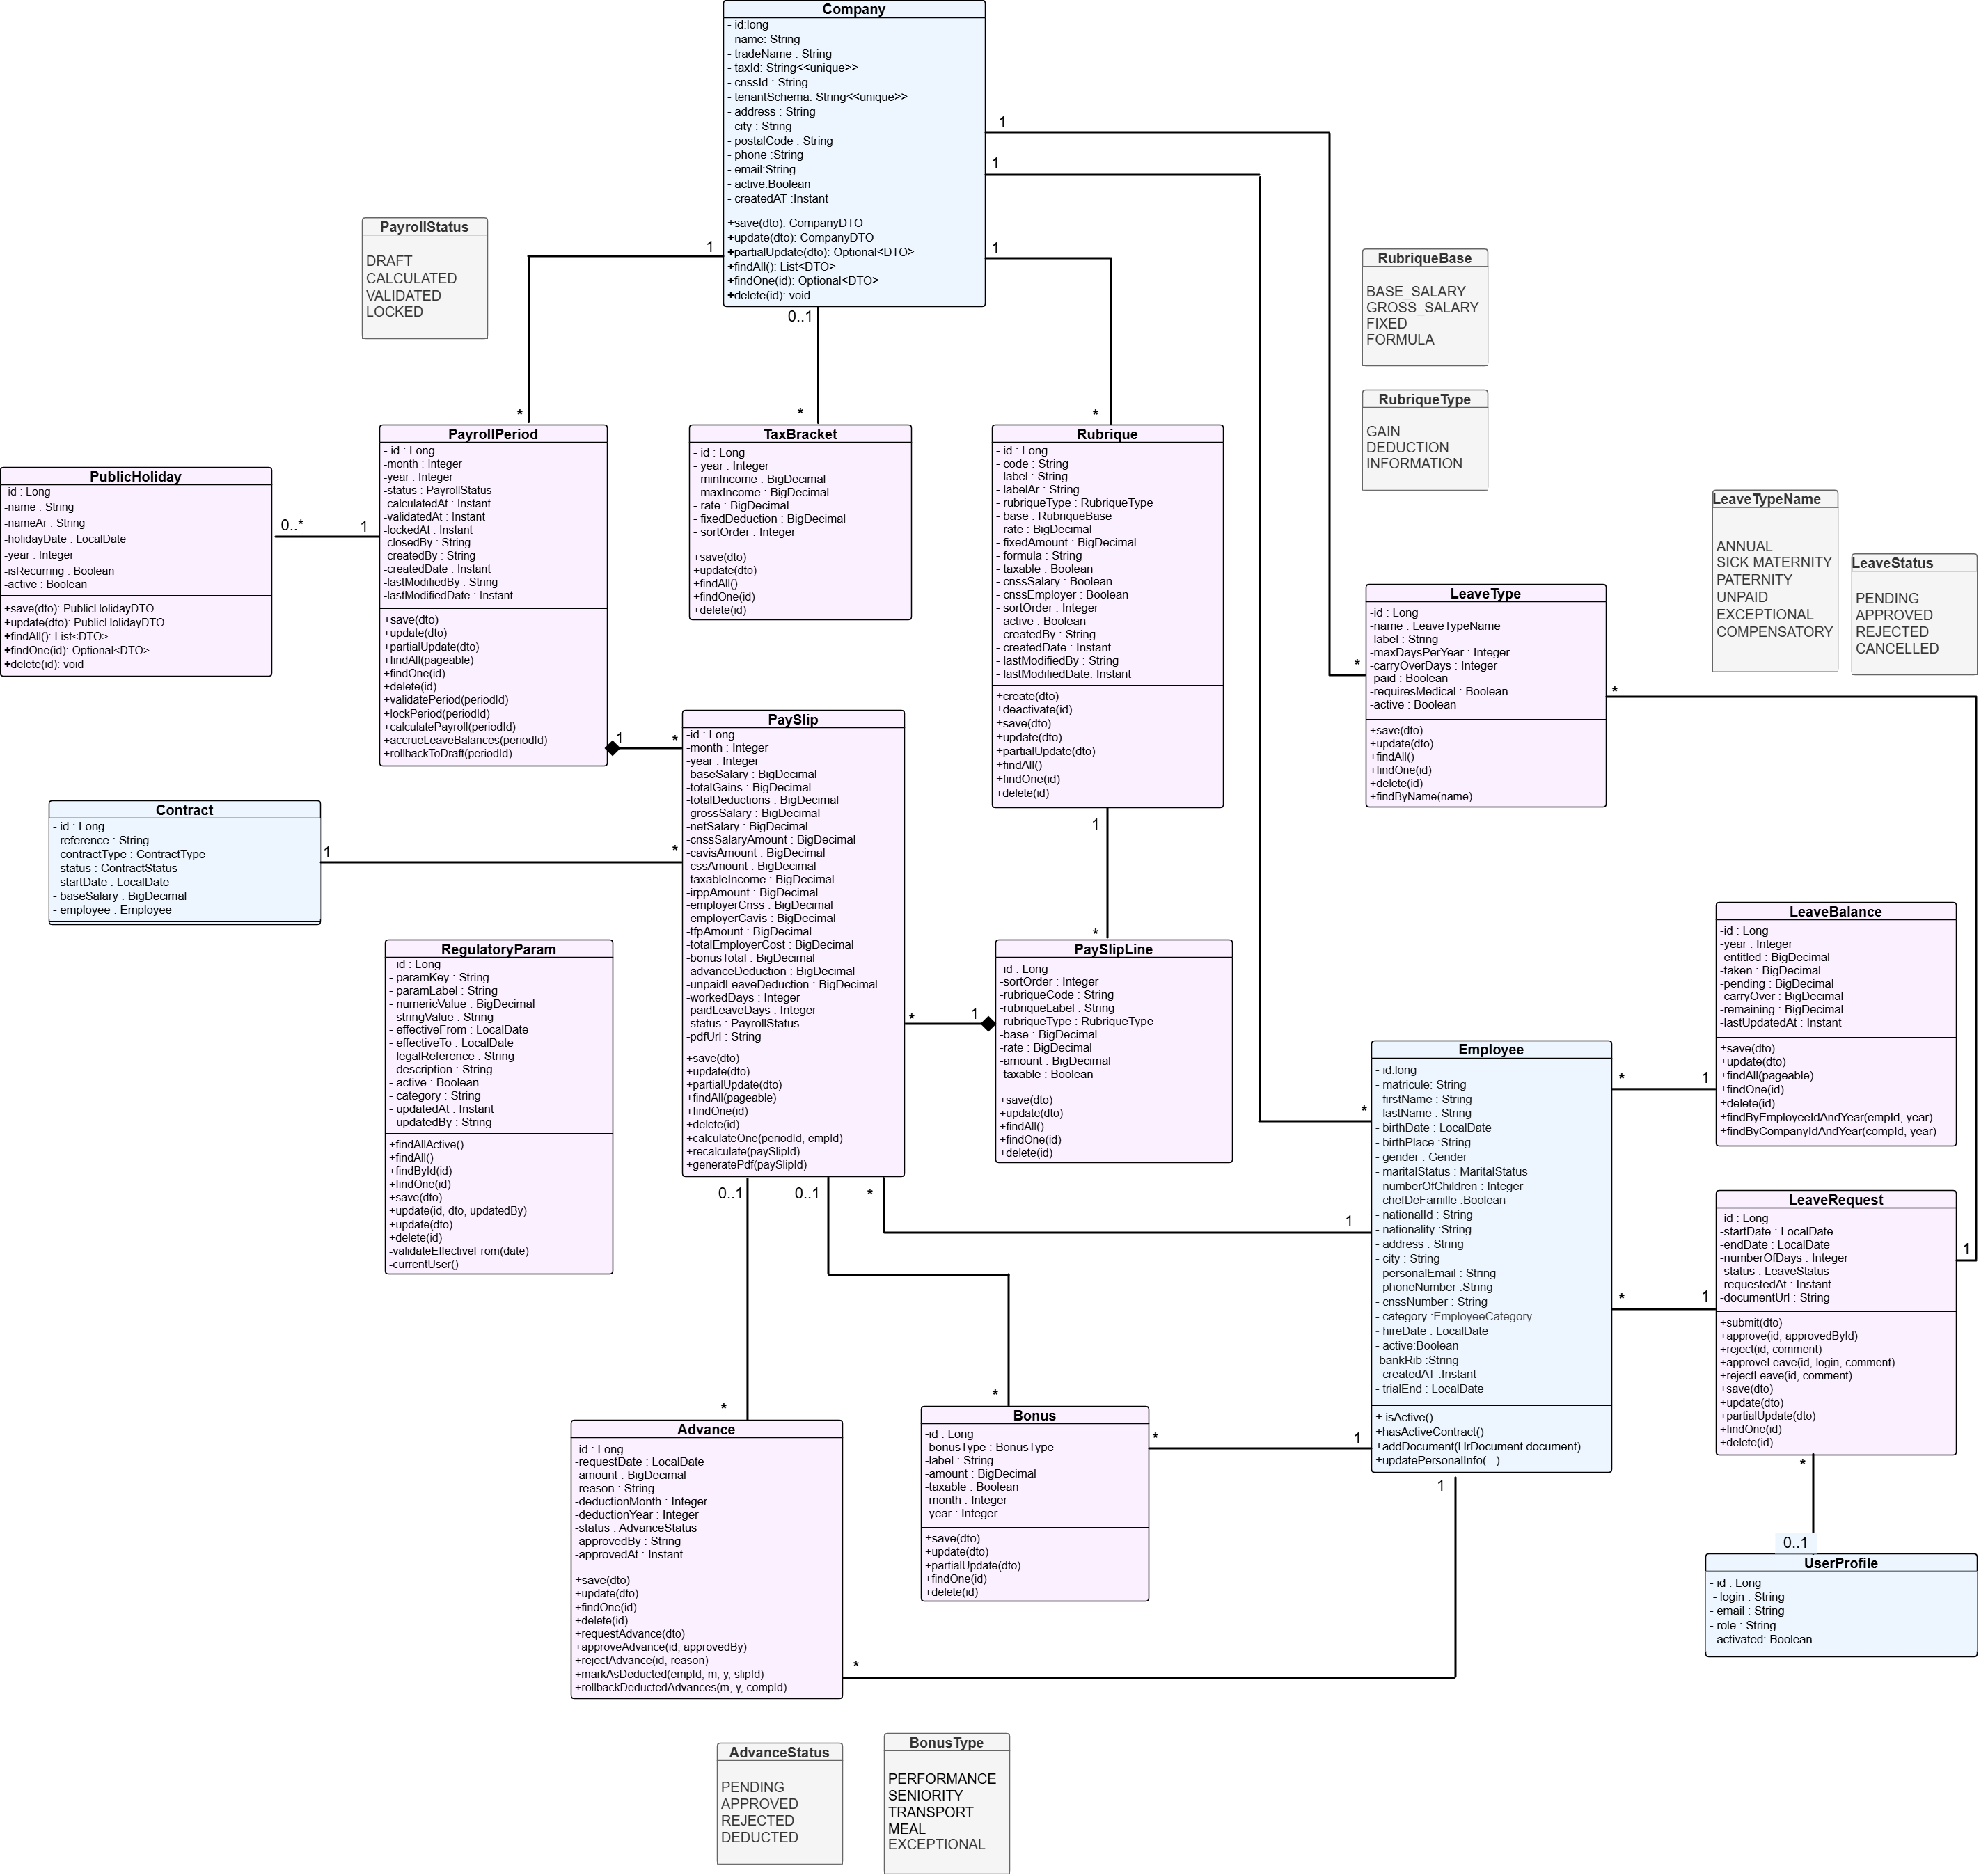
\includegraphics[width=0.99\textwidth]{classes-sprint3.png}
  \caption{Diagramme de classes du Sprint 3 --- PaieZone}
  \label{fig:classes-sprint3}
\end{figure}

Le diagramme de classes du Sprint~3 (Figure~\ref{fig:classes-sprint3})
enrichit le modèle du Sprint~2 en introduisant les entités nécessaires
au moteur de paie et à la gestion des congés.

\textbf{Entités du cycle de paie~:}
\begin{itemize}[label=\textbullet, leftmargin=0.6cm]
    \item \textbf{RegulatoryParam}~: stocke les paramètres
          réglementaires versionnés (clé, valeur numérique, date d'entrée
          en vigueur, référence légale). Plusieurs enregistrements peuvent
          coexister pour un même paramètre~; le moteur utilise toujours
          la version active à la date de la période.

    \item \textbf{TaxBracket}~: modélise les tranches progressives
          du barème IRPP (borne inférieure, borne supérieure, taux
          d'imposition, déduction fixe). Cette entité est chargée
          dynamiquement à chaque calcul de bulletin.

    \item \textbf{PayrollPeriod}~: représente une période mensuelle
          de paie (mois, année, statut~: OUVERTE /
          CALCULÉE / CLÔTURÉE, horodatage de clôture
          lockedAt). Elle est liée à la Compan
          par une association de composition.

    \item \textbf{Rubrique}~: paramètre de calcul configuré par
          la société (type~: GAIN ou RETENU, base
          de calcul, montant ou pourcentage). Elle structure les éléments
          du bulletin au-delà des cotisations légales.

    \item \textbf{Bonus}~: prime individuelle ou collective
          affectée à un employé pour une période donnée (montant, type,
          statut). Agrégée dans le brut lors du calcul.

    \item \textbf{Advance}~: demande d'avance sur salaire.
          Cycle~: PENDING~$\rightarrow$~APPROVED
          / REJECTED~$\rightarrow$~DEDUCTED lors
          du calcul du bulletin.

    \item \textbf{PaySlip}~: bulletin de paie calculé. Stocke
          tous les montants,

    \item \textbf{PaySlipLine}~: détail ligne par ligne du
          bulletin (libellé, base, taux, montant gain/retenue), permettant
          l'affichage du bulletin PDF complet.
\end{itemize}

\textbf{Entités de gestion des congés~:}
\begin{itemize}[label=\textbullet, leftmargin=0.6cm]
    \item \textbf{LeaveType}~: type de congé paramétrable
          (annuel légal, maladie, sans solde, maternité) avec quota
          annuel en jours.

    \item \textbf{LeaveBalance}~: solde de congés en temps réel
          par employé et par type de congé.

    \item \textbf{LeaveRequest}~: demande de congé soumise par
          un employé (dates, type, statut).

    \item \textbf{PublicHoliday}~: jours fériés tunisiens
          paramétrables, automatiquement exclus du décompte des jours
          de congé.
\end{itemize}

% -----------------------------------------------------------
\subsection{Diagrammes de séquences}
% -----------------------------------------------------------

Les diagrammes de séquences suivants modélisent la dynamique des
cas d'utilisation principaux du Sprint~3 selon l'architecture
N-Tiers à trois couches de PaieZone.

% -----------------------------------------------------------
\subsubsection{Diagramme de séquence : Lancer le calcul des bulletins de paie}
% -----------------------------------------------------------

La figure~\ref{fig:seq-calcul} illustre le flux de calcul automatisé
des bulletins de paie pour une période donnée.

\begin{figure}[H]
  \centering
  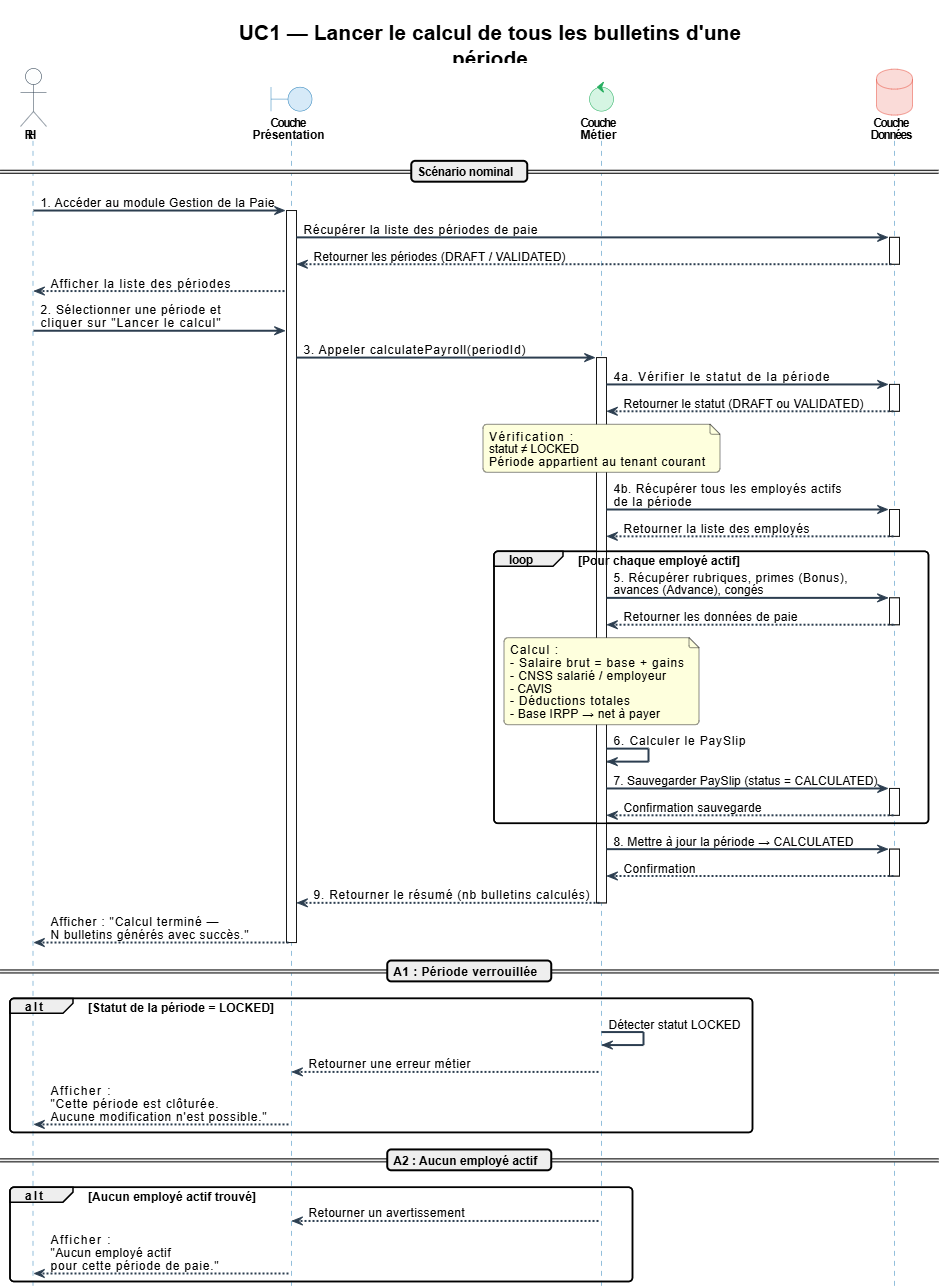
\includegraphics[width=0.78\textwidth]{seq-sp3-uc1.png}
  \caption{Diagramme de séquence --- Lancer le calcul des bulletins de paie}
  \label{fig:seq-calcul}
\end{figure}

Ce diagramme illustre l'ordonnancement du traitement de la paie,
pilier central du Sprint~3. Le moteur de calcul automatise la
transformation des données contractuelles en bulletins de paie nets,
en appliquant rigoureusement les barèmes réglementaires à l'ensemble
des employés actifs. Ce flux garantit l'intégrité des résultats
financiers ainsi que la mise à jour cohérente des statuts de la
période de paie.

% -----------------------------------------------------------
\subsubsection{Diagramme de séquence : Clôturer une période de paie}
% -----------------------------------------------------------

La figure~\ref{fig:seq-cloture} illustre le flux de clôture d'une
période de paie.

\begin{figure}[H]
  \centering
  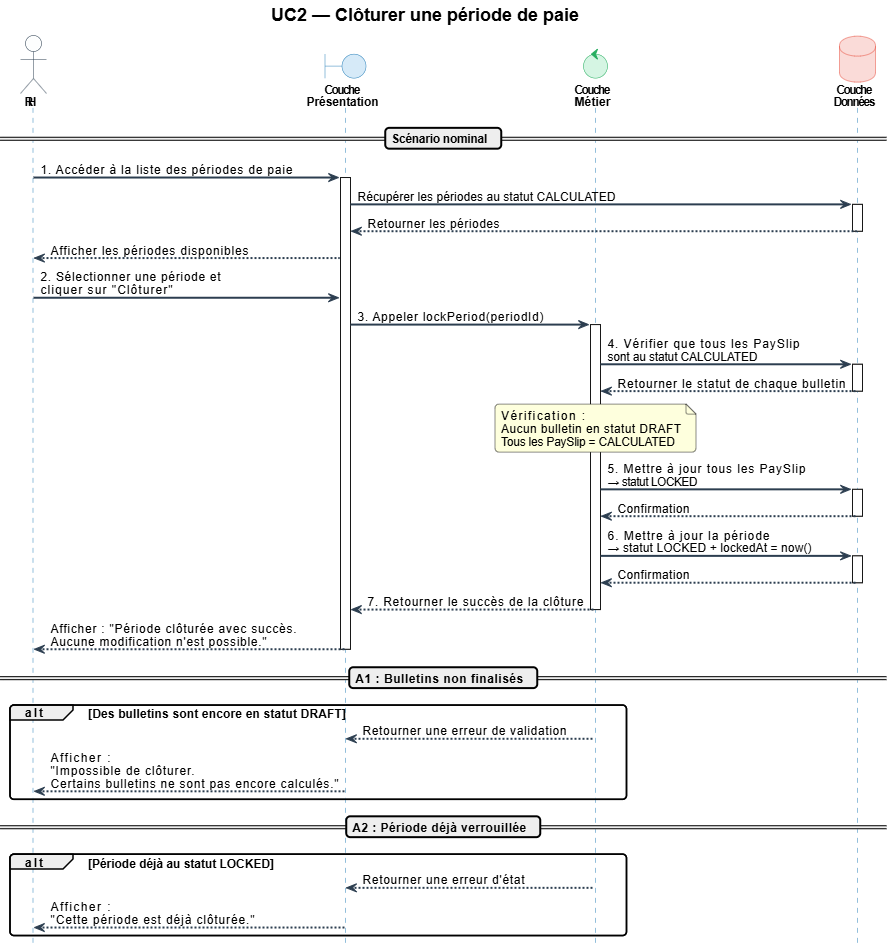
\includegraphics[width=0.90\textwidth]{seq-sp3-uc2.png}
  \caption{Diagramme de séquence --- Clôturer une période de paie }
  \label{fig:seq-cloture}
\end{figure}

Ce diagramme détaille le processus de clôture définitive d'une période
de paie, garantissant l'intégrité et l'immuabilité des résultats
financiers. Le flux assure la validation préalable de l'état des
bulletins avant d'opérer un verrouillage global, interdisant ainsi
toute modification ultérieure des données de paie.

% -----------------------------------------------------------
\subsubsection{Diagramme de séquence : Demande et traitement d’une avance sur salaire}
% -----------------------------------------------------------

La figure~\ref{fig:seq-avance2} illustre le flux de demande et de
traitement d'une avance sur salaire.

\begin{figure}[H]
  \centering
  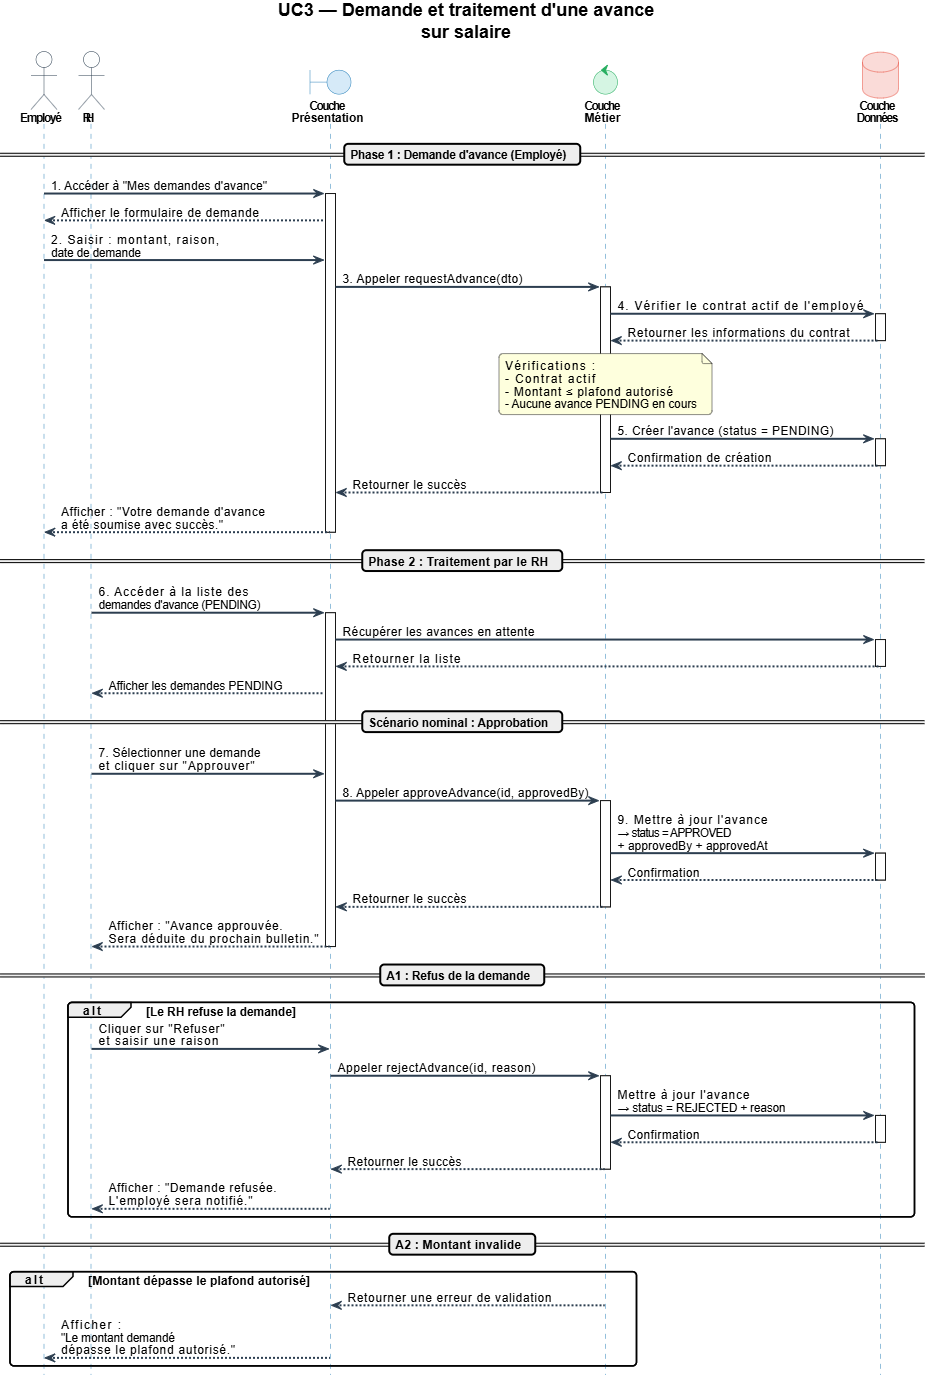
\includegraphics[width=0.775\textwidth]{seq-sp3-uc3.png}
  \caption{Diagramme de séquence --- Demande et traitement d'une avance sur salaire}
  \label{fig:seq-avance2}
\end{figure}

Ce diagramme illustre le processus de gestion des avances sur salaire.
Le flux débute par la soumission de la demande par l'\textbf{Employé},
soumise à des contrôles d'éligibilité automatiques (contrat actif,
plafond autorisé), et se conclut par la décision du \textbf{RH}
(approbation ou refus). L'approbation déclenche l'intégration automatique
de l'avance dans le prochain cycle de paie avec passage au statut DEDUCTE lors du calcul du bulletin.

% ============================================================
\section{Étude et réalisation}
\label{sec:s3-realisation}
% ============================================================

Cette section détaille les réalisations concrètes du troisième sprint,
marquant l'aboutissement du c\oe{}ur métier de la plateforme. Les travaux
ont porté sur~: l'implémentation du moteur de calcul de paie conforme
à la Loi de Finances 2026, le traitement en lot transactionnel des
bulletins, la génération PDF
des bulletins, la configuration des paramètres
réglementaires versionnés, et l'automatisation des processus de
gestion des congés avec mise à jour dynamique des soldes.

% -----------------------------------------------------------
\subsection{Gestion des paramètres réglementaires}
% -----------------------------------------------------------

\begin{figure}[H]
  \centering
  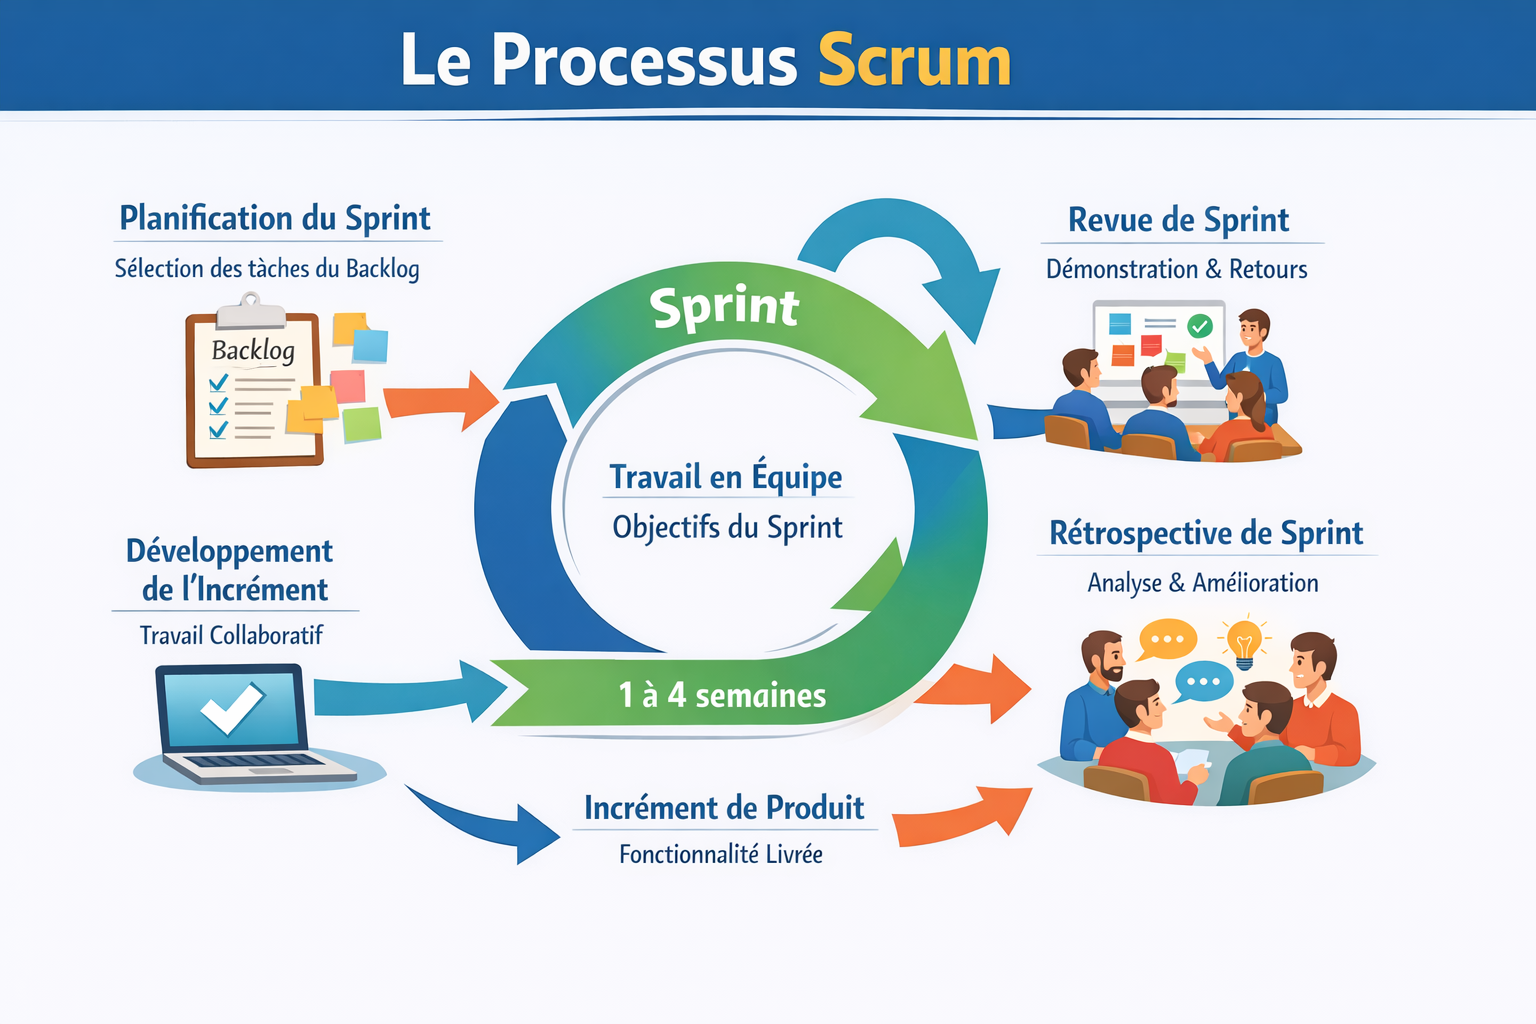
\includegraphics[width=0.70\textwidth]{scrum.png}
  \caption{Interface de gestion des paramètres réglementaires}
  \label{fig:ui-params}
\end{figure}

La figure~\ref{fig:ui-params} présente l'interface de gestion des
paramètres réglementaires, accessible exclusivement au Super Admin.
Elle permet de consulter, ajouter et modifier les constantes légales
(taux CNSS, CAVIS, CSS, TFP, barème IRPP, SMIG) sans redéploiement.
Chaque modification est horodatée et tracée dans le journal d'audit.

% -----------------------------------------------------------
\subsection{Gestion des périodes de paie}
% -----------------------------------------------------------

\begin{figure}[H]
  \centering
  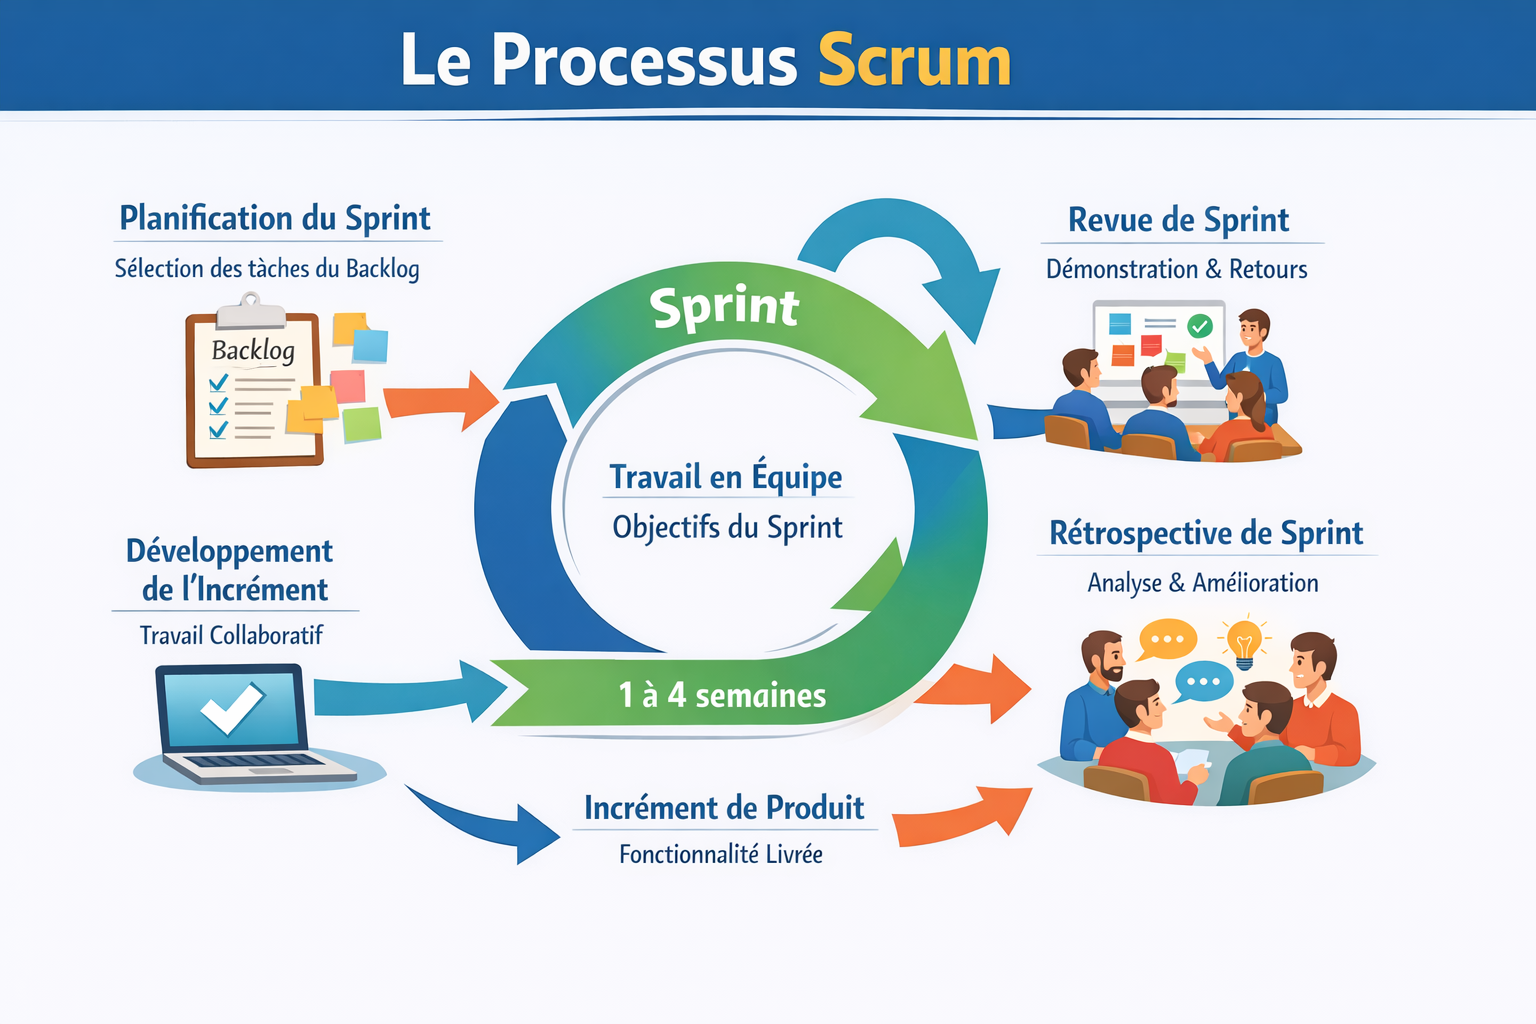
\includegraphics[width=0.70\textwidth]{scrum.png}
  \caption{Interface de gestion des périodes de paie}
  \label{fig:ui-periodes}
\end{figure}

La figure~\ref{fig:ui-periodes} présente le module de gestion des
périodes de paie. Le RH peut créer une nouvelle période mensuelle,
suivre son évolution selon trois statuts successifs~:
OUVERTE (calcul possible), CALCULÉE (bulletins
générés, clôture autorisée) et CLÔTURÉE (verrouillage
définitif). Ce mécanisme garantit
l'immuabilité des données de paie validées.

% -----------------------------------------------------------
\subsection{Calcul et visualisation des bulletins de paie}
% -----------------------------------------------------------

\begin{figure}[H]
  \centering
  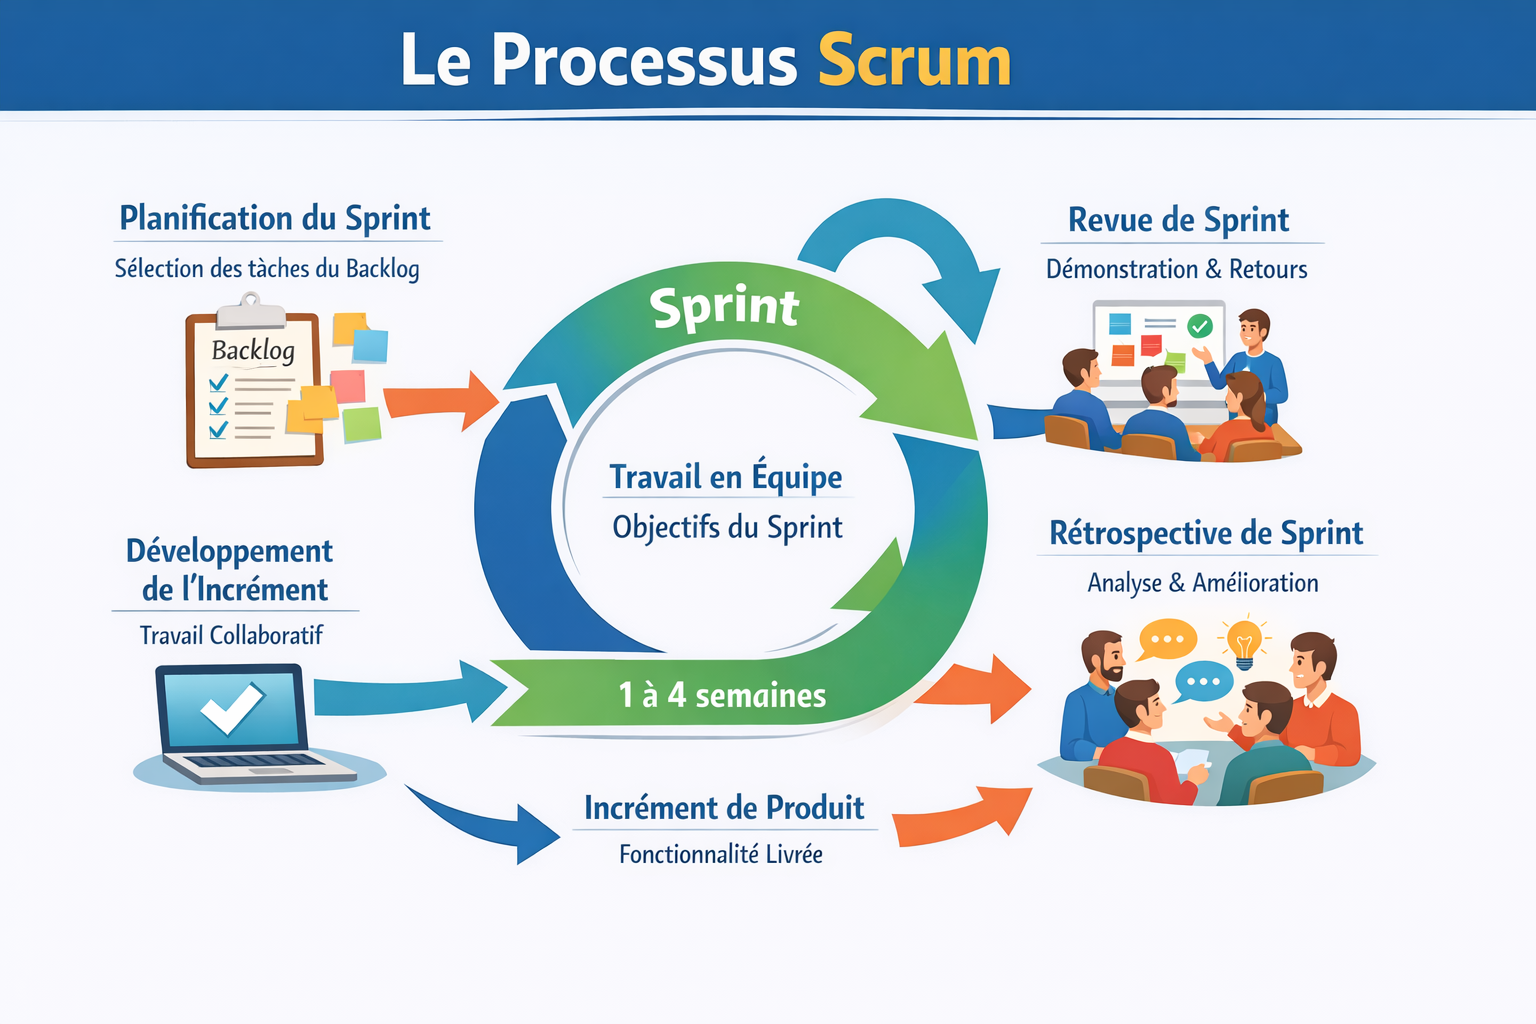
\includegraphics[width=0.70\textwidth]{scrum.png}
  \caption{Interface de calcul et de visualisation des bulletins de paie}
  \label{fig:ui-bulletins}
\end{figure}

La figure~\ref{fig:ui-bulletins} présente l'interface de calcul des
bulletins de paie. Le RH lance le calcul en lot, visualise les bulletins
générés avec le détail des cotisations et du montant net, et peut
exporter chaque bulletin en PDF ou déclencher l'envoi groupé.

% -----------------------------------------------------------
\subsection{Gestion des primes et des avances}
% -----------------------------------------------------------

\begin{figure}[H]
  \centering
  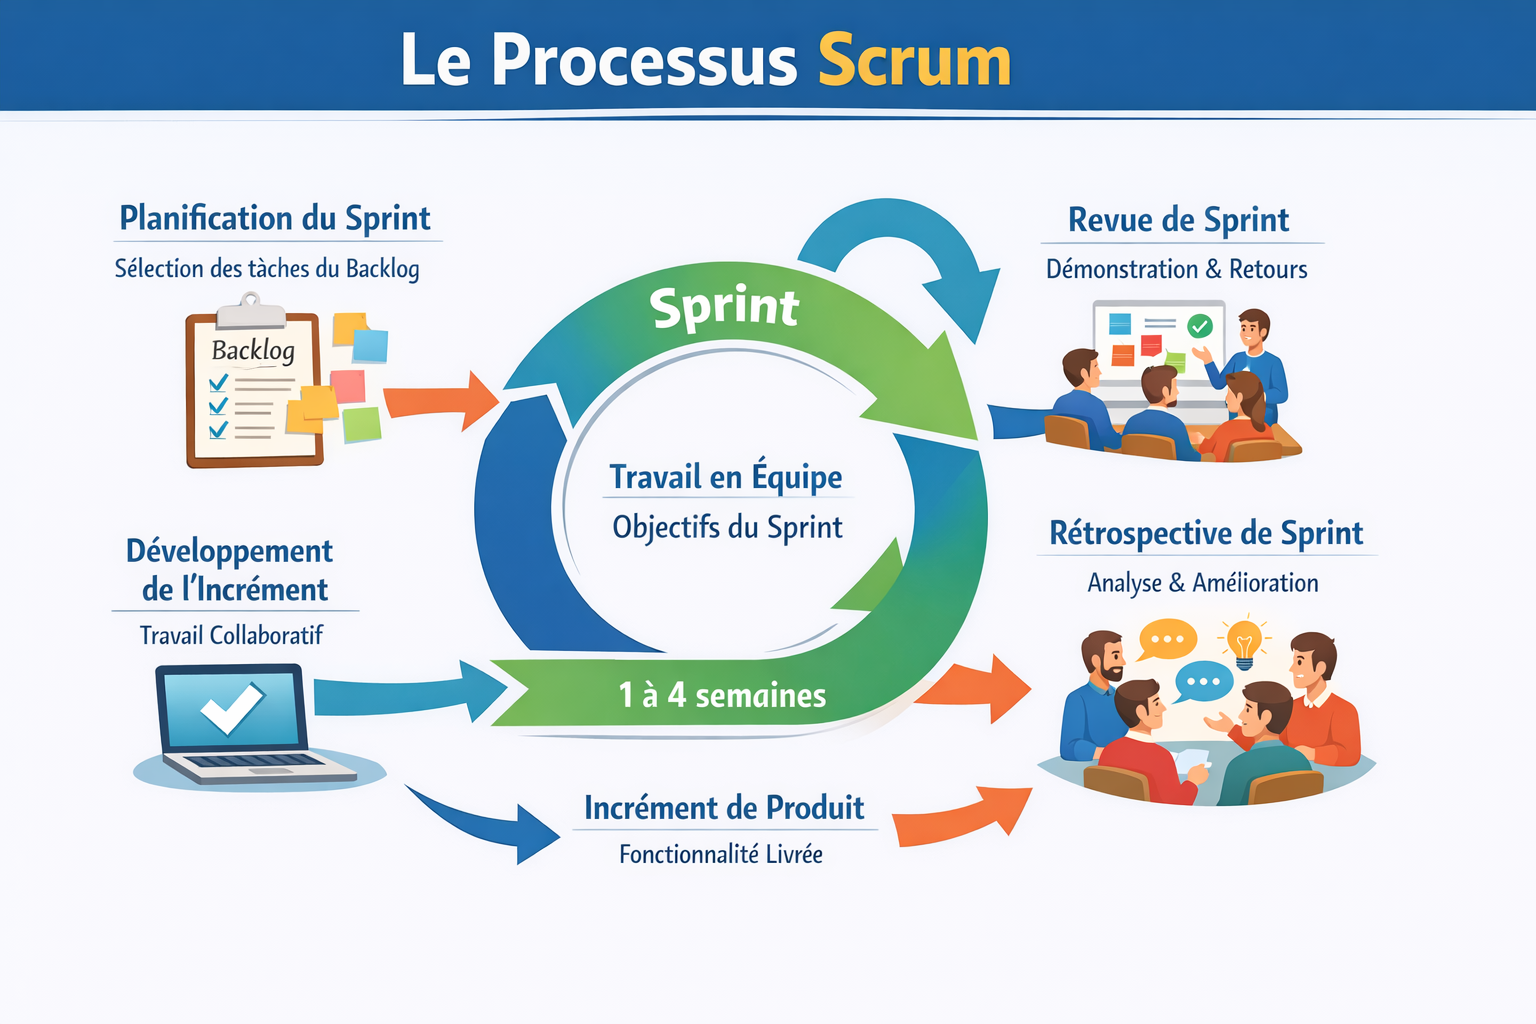
\includegraphics[width=0.70\textwidth]{scrum.png}
  \caption{Interface de gestion des primes et des avances}
  \label{fig:ui-primes}
\end{figure}

La figure~\ref{fig:ui-primes} présente le module de gestion des
éléments variables de la paie. Le RH peut ajouter des primes
individuelles ou collectives et traiter les demandes d'avance soumises
par les employés (validation ou refus). Les montants validés sont
automatiquement intégrés dans le calcul du bulletin de la période
courante.

% -----------------------------------------------------------
\subsection{Gestion des congés et des absences}
% -----------------------------------------------------------

\begin{figure}[H]
  \centering
  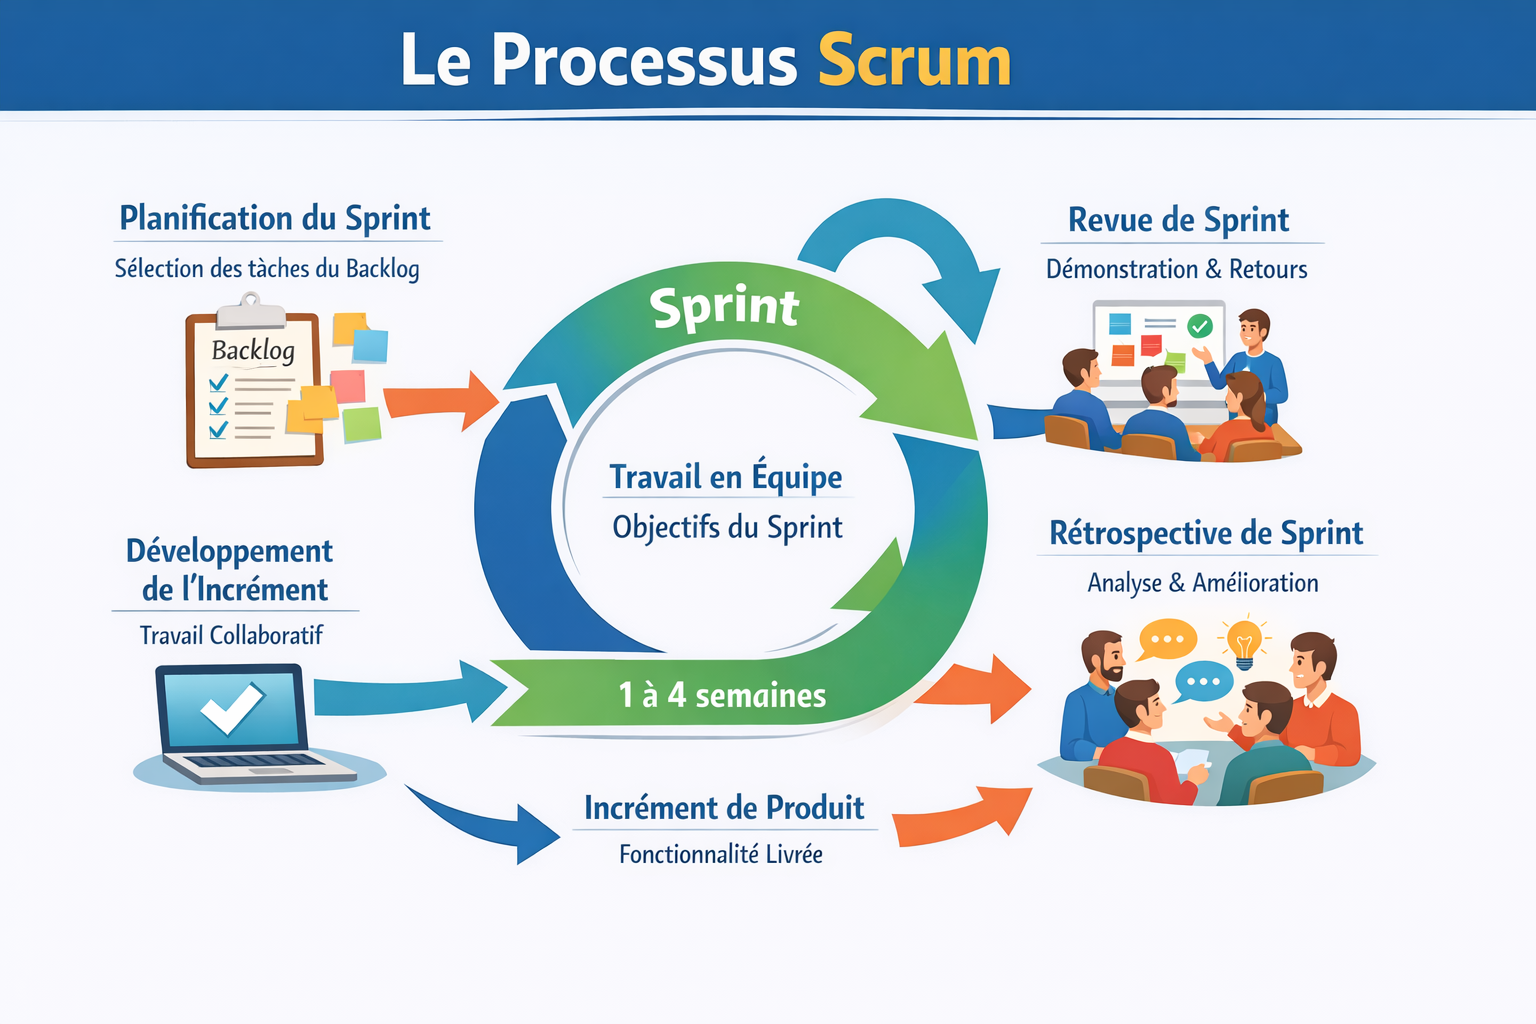
\includegraphics[width=0.70\textwidth]{scrum.png}
  \caption{Interface de gestion des congés et des absences}
  \label{fig:ui-conges}
\end{figure}

La figure~\ref{fig:ui-conges} présente le module de gestion des congés.
L'Employé dispose d'un calendrier interactif pour soumettre ses demandes
et consulter son solde en temps réel. Le RH accède à un tableau de bord
des demandes en attente, avec les actions de validation et de refus.
Les jours fériés configurés sont automatiquement exclus du décompte
des jours de congé.

% ============================================================
\section{Tests et Validation}
\label{sec:s3-tests}
% ============================================================

La phase de tests du Sprint~3 accorde une importance particulière
à la fiabilité du moteur de calcul de paie, dont les résultats ont
des implications financières et légales directes pour les sociétés
clientes de PaieZone.

% -----------------------------------------------------------
\subsection{Plan de tests}
% -----------------------------------------------------------

Trois types de tests ont été mis en \oe{}uvre~: les \textbf{tests
unitaires} du moteur de calcul, les \textbf{tests
d'intégration} des flux métier complets, et les \textbf{tests
fonctionnels} des interfaces Angular.

Le tableau~\ref{tab:tests-sprint3} présente le plan de tests du Sprint~3.

\begin{small}
\renewcommand{\arraystretch}{1.3}
\begin{longtable}{|>{\bfseries}p{1.5cm}|p{1.2cm}|p{2cm}|p{4.5cm}|p{2.5cm}|p{1.5cm}|}

\hline
\rowcolor[gray]{0.9}\textbf{ID} & \textbf{US} & \textbf{Type} &
\textbf{Description} & \textbf{Résultat attendu} & \textbf{Statut} \\ \hline
\endfirsthead
\hline
\rowcolor[gray]{0.9}\textbf{ID} & \textbf{US} & \textbf{Type} &
\textbf{Description} & \textbf{Résultat attendu} & \textbf{Statut} \\ \hline
\endhead
\hline
\endfoot
\hline
\caption{Plan de tests du Sprint 3 }
\label{tab:tests-sprint3} 
\endlastfoot
TC-01 & 10.2 & Unitaire & Ajout d'un paramètre avec un taux valide & Paramètre enregistré, audit tracé & OK \\ \hline
TC-02 & 10.3 & Unitaire & Modification avec taux hors bornes & Erreur de validation bloquante & OK \\ \hline
TC-03 & 11.1 & Intégration & Création d'une période de paie & Période créée au statut \texttt{OUVERTE} & OK \\ \hline
TC-04 & 11.3 & Intégration & Clôture d'une période & Statut \texttt{CLÔTURÉE}, modifications rejetées & OK \\ \hline
TC-05 & 11.4 & Unitaire & Calcul du salaire net avec prime et avance & Net = Brut + Prime - CNSS - CAVIS - CSS - IRPP - Avance & OK \\ \hline
TC-06 & 11.4 & Intégration & Calcul par lot pour 10 employés & 10 bulletins générés sans erreur & OK \\ \hline
TC-07 & 11.4 & Intégration & Calcul sans paramètres configurés & Erreur bloquante + message explicite & OK \\ \hline
TC-08 & 11.12 & Fonctionnel & Génération du bulletin PDF & PDF conforme au template réglementaire & OK \\ \hline
TC-09 & 11.13 & Fonctionnel & Génération du fichier CNSS & Fichier au format réglementaire & OK \\ \hline
TC-10 & 12.2 & Intégration & Demande de congé avec solde insuffisant & Demande bloquée & OK \\ \hline
TC-11 & 12.3 & Intégration & Validation d'un congé & Solde décrémenté + notification envoyée & OK \\ \hline
TC-12 & 12.5 & Intégration & Congé couvrant un jour férié & Jour férié exclu du décompte & OK \\ \hline
\end{longtable}
\end{small}
\renewcommand{\arraystretch}{1.0}

La stratégie de validation du Sprint~3 s'est concentrée sur la fiabilité
du moteur de calcul et la conformité légale des documents produits. Une
attention particulière a été portée aux scénarios critiques, tels que
la gestion simultanée des éléments variables de paie, l'intégrité des
calculs en l'absence de paramètres configurés, et l'irréversibilité du
processus de clôture.

% -----------------------------------------------------------
\subsection{Tests automatisés}
% -----------------------------------------------------------

Le Sprint~3 concentre les calculs financiers les plus critiques de \pz{}
(CNSS, IRPP, CSS, génération PDF). Deux classes de tests automatisés ont
été développées avec JUnit~5 et Mockito.

\paragraph{TunisianTaxServiceTest --- 8 cas de test}
Ces tests vérifient la conformité des calculs fiscaux à la
\textbf{Loi de Finances 2026} (JORT n°3-2026). Chaque taux est testé
indépendamment pour éviter toute régression lors des mises à jour réglementaires
annuelles~:

\renewcommand{\arraystretch}{1.2}
\begin{small}
\begin{xltabular}{\textwidth}{|c|X|p{4cm}|c|}
\hline
\rowcolor[gray]{0.9}
\textbf{ID} & \textbf{Scénario} & \textbf{Résultat attendu} & \textbf{Statut} \\ \hline
\endfirsthead \hline
\rowcolor[gray]{0.9}
\textbf{ID} & \textbf{Scénario} & \textbf{Résultat attendu} & \textbf{Statut} \\ \hline
\endhead \hline \endfoot \hline
\caption{Tests automatisés --- TunisianTaxServiceTest}\label{tab:auto-tax}\endlastfoot
TA-S3-01 & CNSS salarial, salaire 1~500~TND (sous plafond)
    & 145,200 TND (9,68\,\%) & \textcolor{green!60!black}{\textbf{OK}} \\ \hline
TA-S3-02 & CNSS salarial, salaire 7~000~TND (au-dessus plafond 5~000 TND)
    & 484,000 TND (plafonné) & \textcolor{green!60!black}{\textbf{OK}} \\ \hline
TA-S3-03 & CSS à 0,5\,\% sur revenu imposable 1~806,400 TND
    & 9,032 TND & \textcolor{green!60!black}{\textbf{OK}} \\ \hline
TA-S3-04 & IRPP annuel $<$ 5~000 TND (tranche exonérée)
    & 0 TND & \textcolor{green!60!black}{\textbf{OK}} \\ \hline
TA-S3-05 & IRPP dans la tranche à 15\,\%
    & Montant conforme au barème LF 2026 & \textcolor{green!60!black}{\textbf{OK}} \\ \hline
TA-S3-06 & Chef de famille avec 2 enfants paie moins qu'un célibataire
    & IRPP chef $<$ IRPP célibataire & \textcolor{green!60!black}{\textbf{OK}} \\ \hline
TA-S3-07 & Calcul intégré : 2~000 TND, marié, 2~enfants
    & Net = 1~543,685 TND & \textcolor{green!60!black}{\textbf{OK}} \\ \hline
TA-S3-08 & IRPP mensuel dans la tranche à 25\,\%
    & Montant conforme au barème & \textcolor{green!60!black}{\textbf{OK}} \\ \hline
\end{xltabular}
\end{small}
\renewcommand{\arraystretch}{1.0}

\paragraph{PdfExportServiceTest --- 8 cas de test}
Ces tests vérifient que chaque PDF généré est un fichier valide
(signature binaire \texttt{\%PDF}) et que les cas d'erreur sont
correctement gérés (bulletin introuvable $\rightarrow$
\texttt{EntityNotFoundException}).

\renewcommand{\arraystretch}{1.2}
\begin{small}
\begin{xltabular}{\textwidth}{|c|X|p{4cm}|c|}
\hline
\rowcolor[gray]{0.9}
\textbf{ID} & \textbf{Scénario} & \textbf{Résultat attendu} & \textbf{Statut} \\ \hline
\endfirsthead \hline
\rowcolor[gray]{0.9}
\textbf{ID} & \textbf{Scénario} & \textbf{Résultat attendu} & \textbf{Statut} \\ \hline
\endhead \hline \endfoot \hline
\caption{Tests automatisés --- PdfExportServiceTest}\label{tab:auto-pdf}\endlastfoot
TA-S3-09 & Génération bulletin pour un employé valide
    & PDF non vide, commence par \texttt{\%PDF} & \textcolor{green!60!black}{\textbf{OK}} \\ \hline
TA-S3-10 & Génération bulletin, ID inexistant
    & \texttt{EntityNotFoundException} levée & \textcolor{green!60!black}{\textbf{OK}} \\ \hline
TA-S3-11 & Génération bulletin avec heures supplémentaires
    & PDF valide incluant la ligne HS & \textcolor{green!60!black}{\textbf{OK}} \\ \hline
TA-S3-12 & Génération attestation de travail
    & PDF valide & \textcolor{green!60!black}{\textbf{OK}} \\ \hline
TA-S3-13 & Génération attestation, employé inconnu
    & \texttt{EntityNotFoundException} levée & \textcolor{green!60!black}{\textbf{OK}} \\ \hline
TA-S3-14 & Journal de paie pour 1 bulletin
    & PDF valide & \textcolor{green!60!black}{\textbf{OK}} \\ \hline
TA-S3-15 & Journal de paie sans aucun bulletin
    & \texttt{IllegalStateException} levée & \textcolor{green!60!black}{\textbf{OK}} \\ \hline
TA-S3-16 & Génération en masse (bulk) pour 2 bulletins
    & PDF fusionné valide & \textcolor{green!60!black}{\textbf{OK}} \\ \hline
\end{xltabular}
\end{small}
\renewcommand{\arraystretch}{1.0}

\textbf{Résultat global Sprint~3~:} 16/16 tests automatisés passés
(\textcolor{green!60!black}{\textbf{OK}}), couverture estimée à
\textbf{85\,\%} pour \texttt{TunisianTaxService} et \textbf{65\,\%}
pour \texttt{PdfExportService}.

% ============================================================
\section{Rituels Agiles et Clôture du Sprint}
\label{sec:s3-rituels}
% ============================================================

En parfaite adéquation avec le cadre méthodologique Scrum, le Sprint 3 s'est conclu par l'exécution des rituels de clôture standards. Ces rituels incluent la revue de sprint, dédiée à la validation des livrables en présence des parties prenantes, et la rétrospective, axée sur l'analyse critique et l'amélioration continue des processus de l'équipe de développement.

% -----------------------------------------------------------
\subsection{Revue du Sprint (Sprint Review)}
% -----------------------------------------------------------

La Sprint Review a permis de valider les livrables du Sprint~3 devant
le Product Owner~: moteur de calcul de paie, génération des bulletins
PDF et du fichier CNSS, ainsi que le module de gestion des congés.
L'ensemble des vingt-deux User Stories a été accepté.

% -----------------------------------------------------------
\subsection{Rétrospective du Sprint (Sprint Retrospective)}

L'équipe a mené une réflexion collective sur le déroulement du Sprint~3~:

\begin{itemize}[label=\textbullet, leftmargin=0.6cm]

    \item \textbf{Ce qui a bien fonctionné~:}
    \begin{itemize}[label=\textbullet, leftmargin=0.8cm]
        \item Le calcul en lot transactionnel a démontré sa fiabilité pour
              le traitement simultané de l'ensemble des bulletins de paie.
        \item La communication fluide avec le Product Owner a facilité la
              validation rapide des livrables.
    \end{itemize}

    \item \textbf{Problèmes rencontrés~:}
    \begin{itemize}[label=\textbullet, leftmargin=0.8cm]
        \item La complexité du calcul IRPP par tranches progressives a été
              sous-estimée lors du Sprint Planning.
        \item La validation du format du fichier CNSS a nécessité plusieurs
              cycles de correction en fin de sprint.
    \end{itemize}

    \item \textbf{Actions d'amélioration pour le Sprint~4~:}
    \begin{itemize}[label=\textbullet, leftmargin=0.8cm]
        \item Lors des tests, la nécessité d'intégrer les conventions
              sectorielles (jours ouvrables, primes spécifiques) a été
              identifiée~; cette fonctionnalité sera implémentée dans
              le Sprint~4.
    \end{itemize}

\end{itemize}
% ============================================================
\section*{Conclusion}
\label{sec:s3-conclusion}
\addcontentsline{toc}{section}{Conclusion}
% ============================================================
Ce cinquième chapitre a présenté les travaux du Sprint~3, dédié au
c\oe{}ur métier de PaieZone~RH~: paramétrage réglementaire, calcul
automatisé de la paie et gestion des congés. Les vingt-deux User
Stories ont été validées par le Product Owner. Le chapitre suivant
présente le Sprint~4, qui finalise la plateforme avec la comptabilité
intégrée, les déclarations réglementaires, l'intégration des conventions
sectorielles et le déploiement de l'assistant conversationnel PaieBot.
% ==========================================
% CHAPITRE 6 — CORRIGÉ SELON RAPPORT DE JURY
% ==========================================
\newpage
\chapter{ÉTUDE DU SPRINT 4}


\vspace{2.5cm}

\noindent \textbf{\Large Plan}
\vspace{0.8cm}

\begin{enumerate}[label=\textbf{\arabic*}, leftmargin=1.5cm, labelsep=0.8cm]
    \item[] \hspace*{-1.5cm}\textbf{Introduction}                              \dotfill \pageref{sec:s4-intro}
    \item \textbf{User Stories du quatrième sprint}          \dotfill \pageref{sec:s4-userstories}
    \item \textbf{Backlog du quatrième Sprint}               \dotfill \pageref{sec:s4-backlog}
    \item \textbf{Spécification fonctionnelle du Sprint 4}   \dotfill \pageref{sec:s4-specification}
    \item \textbf{Conception du Sprint 4}                    \dotfill \pageref{sec:s4-conception}
    \item \textbf{Étude et réalisation du Sprint 4}          \dotfill \pageref{sec:s4-realisation}
    \item \textbf{Tests et Validation}                       \dotfill \pageref{sec:s4-tests}
    \item \textbf{Rituels Agiles et Clôture du Sprint}       \dotfill \pageref{sec:s4-rituels}
    \item[] \hspace*{-1.5cm} \textbf{Conclusion}                                \dotfill \pageref{sec:s4-conclusion}
\end{enumerate}

\vfill
\newpage

% ============================================================
\section*{Introduction}
\label{sec:s4-intro}
\addcontentsline{toc}{section}{Introduction}
% ============================================================

S'appuyant sur les acquis du Sprint 3 (moteur de paie et gestion des congés),
 ce chapitre présente les réalisations du quatrième et dernier sprint.
  Ce sprint finalise la plateforme PaieZone RH en intégrant la gestion 
  comptable (export SAGE), la conformité réglementaire (CNSS, CAVIS, IRPP), 
  la production de documents administratifs, et l'assistant conversationnel
   PaieBot, basé sur Ollama/phi3 avec architecture RAG et pipeline Text-to-SQL.
    La démarche agile (User Stories, modélisation UML, conception technique,
     interfaces Angular, tests et clôture) a été maintenue.

% ============================================================
\section{User Stories du quatrième sprint}
\label{sec:s4-userstories}
% ============================================================

Lors de la réunion de planification du Sprint 4, l'équipe Scrum a défini
l'objectif du sprint autour de la valeur métier suivante~:
«~Compléter PaieZone par les fonctionnalités de conformité, de
comptabilité, de génération documentaire et d'assistance
conversationnelle, pour offrir une solution SaaS pleinement
opérationnelle.~». Quatre épics prioritaires ont été sélectionnés
dans le backlog produit pour constituer le périmètre de ce sprint~:

\begin{itemize}[label=\textbullet, leftmargin=0.6cm]
    \item Gestion Comptable
    \item Conformité Réglementaire
    \item Documents Administratifs RH
    \item Assistant Conversationnel RH (PaieBot)
\end{itemize}

Les besoins fonctionnels ont été formalisés sous forme de User Stories
détaillées dans le Tableau~\ref{tab:user-stories-sprint4}.

% CORRECTION : Colonne "Priorité" ajoutée + 2 US chatbot manquantes (16.4, 16.5) + IDs cohérents
\begin{small}
\renewcommand{\arraystretch}{1.4}
\begin{longtable}{@{}p{1.2cm} p{9.5cm} p{2.3cm}@{}}
\caption{User Stories sélectionnées pour le quatrième sprint}
\label{tab:user-stories-sprint4} \\
\toprule
\textbf{ID} & \textbf{User Story} & \textbf{Priorité} \\
\midrule
\endfirsthead
\multicolumn{3}{c}{\tablename~\thetable{} --- suite} \\
\toprule
\textbf{ID} & \textbf{User Story} & \textbf{Priorité} \\
\midrule
\endhead
\bottomrule
\endfoot

13.1 & En tant qu'Admin/RH, je veux configurer le plan comptable,
       afin de structurer les comptes de la société et de garantir
       la cohérence des exports comptables.
     & Haute \\
\addlinespace
13.2 & En tant qu'Admin/RH, je veux exporter les données comptables
       au format SAGE (.csv), afin de les intégrer directement dans
       le logiciel comptable de la société.
     & Haute \\
\addlinespace
14.1 & En tant que RH, je veux générer la déclaration CNSS salarié
       par trimestre, afin de déclarer les cotisations salariales
       à la CNSS~\cite{cnss_reg}.
     & Critique \\
\addlinespace
14.2 & En tant que RH, je veux générer la déclaration CNSS patronal
       par trimestre, afin de déclarer les cotisations patronales~\cite{cnss_reg}.
     & Critique \\
\addlinespace
14.3 & En tant que RH, je veux générer la déclaration CAVIS par
       trimestre, afin de satisfaire aux obligations de la Caisse
       d'Assurance Vieillesse, Invalidité et Survivants.
     & Haute \\
\addlinespace
14.4 & En tant que RH, je veux générer la déclaration IRPP annuelle,
       afin de transmettre les retenues à la source à l'administration
       fiscale tunisienne (DGI)~\cite{lf2026}.
     & Critique \\
\addlinespace
15.1 & En tant que RH, je veux générer une attestation de salaire en
       PDF, afin de la remettre à l'employé à sa demande.
     & Haute \\
\addlinespace
15.2 & En tant que RH, je veux générer un certificat de travail en
       PDF, afin d'attester formellement de la relation contractuelle
       de l'employé avec la société.
     & Haute \\
\addlinespace
16.1 & En tant qu'utilisateur authentifié, je veux accéder à un
       assistant conversationnel RH (PaieBot), afin d'obtenir des
       réponses à mes questions administratives en langage naturel.
     & Haute \\
\addlinespace
16.2 & En tant qu'employé, je veux consulter mes données personnelles
       (salaire net, solde de congés, ancienneté, poste) via le
       chatbot, afin d'y accéder directement sans naviguer dans
       l'application.
     & Haute \\
\addlinespace
16.3 & En tant qu'Admin/RH, je veux interroger les données RH de
       ma société via le chatbot (effectif, masse salariale,
       répartition par département), afin d'obtenir des
       statistiques en langage naturel.
     & Moyenne \\
\addlinespace
16.4 & En tant qu'employé, je veux demander un congé via le chatbot,
       afin d'initier rapidement une demande sans naviguer dans
       les menus.
     & Moyenne \\
\addlinespace
16.5 & En tant qu'utilisateur, je veux poser des questions sur la
       réglementation tunisienne (CNSS, IRPP, code du travail) au
       chatbot, afin d'obtenir des réponses fondées sur les textes
       légaux en vigueur.
     & Moyenne \\

\end{longtable}
\end{small}
\renewcommand{\arraystretch}{1.0}

% ============================================================
\section{Backlog du quatrième Sprint}
\label{sec:s4-backlog}
% ============================================================

Le Backlog du produit de PaieZone, regroupant fonctionnalités et
améliorations, est formalisé en User Stories organisées par thèmes
fonctionnels. Le Tableau~\ref{tab:backlog-sprint4} détaille ce backlog
pour le quatrième sprint, incluant les tâches techniques et leurs
estimations en jours.

\begin{small}
\renewcommand{\arraystretch}{1.4}
\begin{longtable}{|p{2.8cm}|p{6.2cm}|p{6.2cm}|c|}
\caption{Backlog détaillé du quatrième Sprint}
\label{tab:backlog-sprint4} \\
\hline
\rowcolor[gray]{0.9} \textbf{Item} & \textbf{User Story} & \textbf{Tâches} & \makecell{\textbf{Est.}\\\textbf{(j)}} \\ \hline
\endfirsthead
\hline
\rowcolor[gray]{0.9} \textbf{Item} & \textbf{User Story} & \textbf{Tâches} & \makecell{\textbf{Est.}\\\textbf{(j)}} \\ \hline
\endhead
\hline
\endfoot
\hline
\endlastfoot

% ── Gestion Comptable ─────────────────────────────────────
\multirow{2}{*}{\makecell[c]{\textbf{Gestion}\\ \textbf{Comptable}}}
& \textbf{13.1} En tant qu'Admin/RH, je souhaite configurer le plan comptable afin de structurer les comptes de la société.
& \begin{itemize}[leftmargin=*, noitemsep, topsep=0pt]
    \item Concevoir l'interface CRUD du plan comptable (créer, modifier, supprimer des comptes).
    \item Développer l'API REST de gestion du plan comptable.
    \item Tester la cohérence des comptes avec les rubriques de paie.
  \end{itemize}
& \textbf{2} \\ \cline{2-4}

& \textbf{13.2} En tant qu'Admin/RH, je souhaite exporter les données comptables au format SAGE (.csv) afin de les intégrer dans le logiciel comptable.
& \begin{itemize}[leftmargin=*, noitemsep, topsep=0pt]
    \item Implémenter le service de génération du fichier CSV au format SAGE.
    \item Ajouter le bouton « Exporter SAGE (.csv) » dans l'onglet Comptabilité.
    \item Tester la conformité du fichier produit avec le format attendu par SAGE.
  \end{itemize}
& \textbf{2} \\ \hline

% ── Conformité Réglementaire ──────────────────────────────
\multirow{4}{*}{\makecell[c]{\textbf{Conformité}\\ \textbf{Réglementaire}}}
& \textbf{14.1} En tant que RH, je souhaite générer la déclaration CNSS salarié par trimestre.
& \begin{itemize}[leftmargin=*, noitemsep, topsep=0pt]
    \item Agréger les cotisations salariales CNSS par trimestre et par employé.
    \item Développer le service de génération du fichier déclaratif.
    \item Implémenter le bouton de déclenchement dans l'onglet Conformité.
    \item Tester la conformité des montants déclarés avec les bulletins calculés.
  \end{itemize}
& \textbf{2} \\ \cline{2-4}

& \textbf{14.2} En tant que RH, je souhaite générer la déclaration CNSS patronal par trimestre.
& \begin{itemize}[leftmargin=*, noitemsep, topsep=0pt]
    \item Agréger les cotisations patronales CNSS par trimestre et par employé.
    \item Développer le service de génération du fichier déclaratif patronal.
    \item Tester la cohérence des montants avec les paramètres réglementaires.
  \end{itemize}
& \textbf{2} \\ \cline{2-4}

& \textbf{14.3} En tant que RH, je souhaite générer la déclaration CAVIS par trimestre.
& \begin{itemize}[leftmargin=*, noitemsep, topsep=0pt]
    \item Implémenter l'agrégation des cotisations CAVIS trimestrielles.
    \item Développer le service de génération du fichier CAVIS.
    \item Tester la prise en compte correcte des taux CAVIS dans les calculs.
  \end{itemize}
& \textbf{2} \\ \cline{2-4}

& \textbf{14.4} En tant que RH, je souhaite générer la déclaration IRPP annuelle.
& \begin{itemize}[leftmargin=*, noitemsep, topsep=0pt]
    \item Agréger les retenues IRPP sur l'ensemble de l'exercice fiscal.
    \item Développer le service de génération de l'état récapitulatif annuel.
    \item Tester la conformité du document produit avec les exigences de la DGI~\cite{lf2026}.
  \end{itemize}
& \textbf{2} \\ \hline

% ── Documents Administratifs RH ───────────────────────────
\multirow{2}{*}{\makecell[c]{\textbf{Documents}\\ \textbf{Administratifs}\\ \textbf{RH}}}
% CORRECTION : "iText / JasperReports" remplacé par "Flying Saucer (ITextRenderer)"
& \textbf{15.1} En tant que RH, je souhaite générer une attestation de salaire en PDF afin de la remettre à l'employé.
& \begin{itemize}[leftmargin=*, noitemsep, topsep=0pt]
    \item Concevoir le template HTML/CSS de l'attestation de salaire (conformité aux formats légaux tunisiens).
    \item Développer le service de génération PDF via \textbf{Flying Saucer}~\cite{flyingsaucer} (\texttt{ITextRenderer}), en injectant les données du dernier bulletin calculé.
    \item Ajouter le bouton de téléchargement dans la page Employés.
    \item Tester la conformité des données affichées (salaire brut, net, poste, signature société).
  \end{itemize}
& \textbf{2} \\ \cline{2-4}

& \textbf{15.2} En tant que RH, je souhaite générer un certificat de travail en PDF afin d'attester de la relation contractuelle.
& \begin{itemize}[leftmargin=*, noitemsep, topsep=0pt]
    \item Concevoir le template HTML/CSS du certificat de travail (conformité aux formats légaux tunisiens).
    \item Développer le service de génération PDF via \textbf{Flying Saucer}~\cite{flyingsaucer} (\texttt{ITextRenderer}) avec les données contractuelles.
    \item Ajouter le bouton de téléchargement dans la page Employés.
    \item Tester la conformité des informations (dates de contrat, poste, société).
  \end{itemize}
& \textbf{2} \\ \hline

% ── Assistant Conversationnel RH (PaieBot) ────────────────
% CORRECTION : Tâches chatbot complétées avec architecture réelle (4 intentions, Text-to-SQL, RAG, sécurité)
\multirow{3}{*}{\makecell[c]{\textbf{Assistant}\\ \textbf{Conversationnel}\\ \textbf{RH (PaieBot)}}}
& \textbf{16.1} En tant qu'utilisateur authentifié, je souhaite accéder à un assistant conversationnel RH afin d'obtenir des réponses en langage naturel.
& \begin{itemize}[leftmargin=*, noitemsep, topsep=0pt]
    \item Intégrer \textbf{Ollama}~\cite{ollama} (modèle phi3~\cite{phi3}) comme moteur LLM local --- aucune donnée RH ne transite vers des services cloud externes.
    \item Implémenter le pipeline de \textbf{détection d'intention} à quatre catégories~: \texttt{PERSONAL\_SQL}, \texttt{ADMIN\_SQL}, \texttt{LEGAL\_RAG}, \texttt{GENERAL}.
    \item Développer le pipeline \textbf{Text-to-SQL} sécurisé~: génération SQL par phi3 (T=0,05), nettoyage, validation (blocage de DROP/DELETE/ALTER/...), injection CTE multi-tenant (\texttt{SET search\_path}).
    \item Implémenter le système \textbf{RAG}~\cite{rag}~: recherche par mots-clés dans \texttt{KnowledgeDocument}, injection dans le prompt système d'Ollama.
    \item Ajouter la protection anti-hallucination (détection regex sur les réponses phi3) et la protection inter-employés (blocage des requêtes inter-tenant).
    \item Concevoir et implémenter le composant Angular chatbot flottant (\texttt{ChatbotComponent}).
    \item Tester les 4 intentions et les cas limites de sécurité.
  \end{itemize}
& \textbf{3} \\ \cline{2-4}

& \textbf{16.4} En tant qu'employé, je souhaite demander un congé via le chatbot afin d'initier rapidement une demande d'absence.
& \begin{itemize}[leftmargin=*, noitemsep, topsep=0pt]
    \item Implémenter la détection de l'intention « congé » dans le chatbot.
    \item Développer la redirection vers la page de demande de congé dédiée.
    \item Tester le flux complet de détection et de redirection.
  \end{itemize}
& \textbf{2} \\ \cline{2-4}

& \textbf{16.2} En tant qu'employé, je souhaite consulter mes données personnelles via le chatbot afin d'y accéder directement.
& \begin{itemize}[leftmargin=*, noitemsep, topsep=0pt]
    \item Implémenter le pipeline \texttt{PERSONAL\_SQL} pour les requêtes personnelles (salaire, congés, ancienneté, poste).
    \item Développer le service de récupération sécurisée des données employé depuis PostgreSQL~\cite{postgresql}.
    \item Tester le formatage des résultats et l'isolation des données par tenant.
  \end{itemize}
& \textbf{2} \\ \hline

\end{longtable}
\end{small}
\renewcommand{\arraystretch}{1.0}
\normalsize

% ============================================================
\section{Spécification fonctionnelle du quatrième Sprint}
\label{sec:s4-specification}
% ============================================================

La modélisation fonctionnelle du Sprint 4 de PaieZone repose sur des
diagrammes de cas d'utilisation UML~\cite{uml}, offrant une représentation visuelle
du périmètre fonctionnel, complétés par des descriptions textuelles
structurées détaillant les scénarios d'interaction pour chaque cas
d'utilisation majeur.

% -----------------------------------------------------------
\subsection{Diagramme de cas d'utilisation du quatrième Sprint}
% -----------------------------------------------------------

La Figure~\ref{fig:use-case-sp4} présente le diagramme de cas
d'utilisation global du Sprint 4 de PaieZone.

\newpage

\begin{figure}[H]
    \vspace*{-0.18cm}
    \centering
    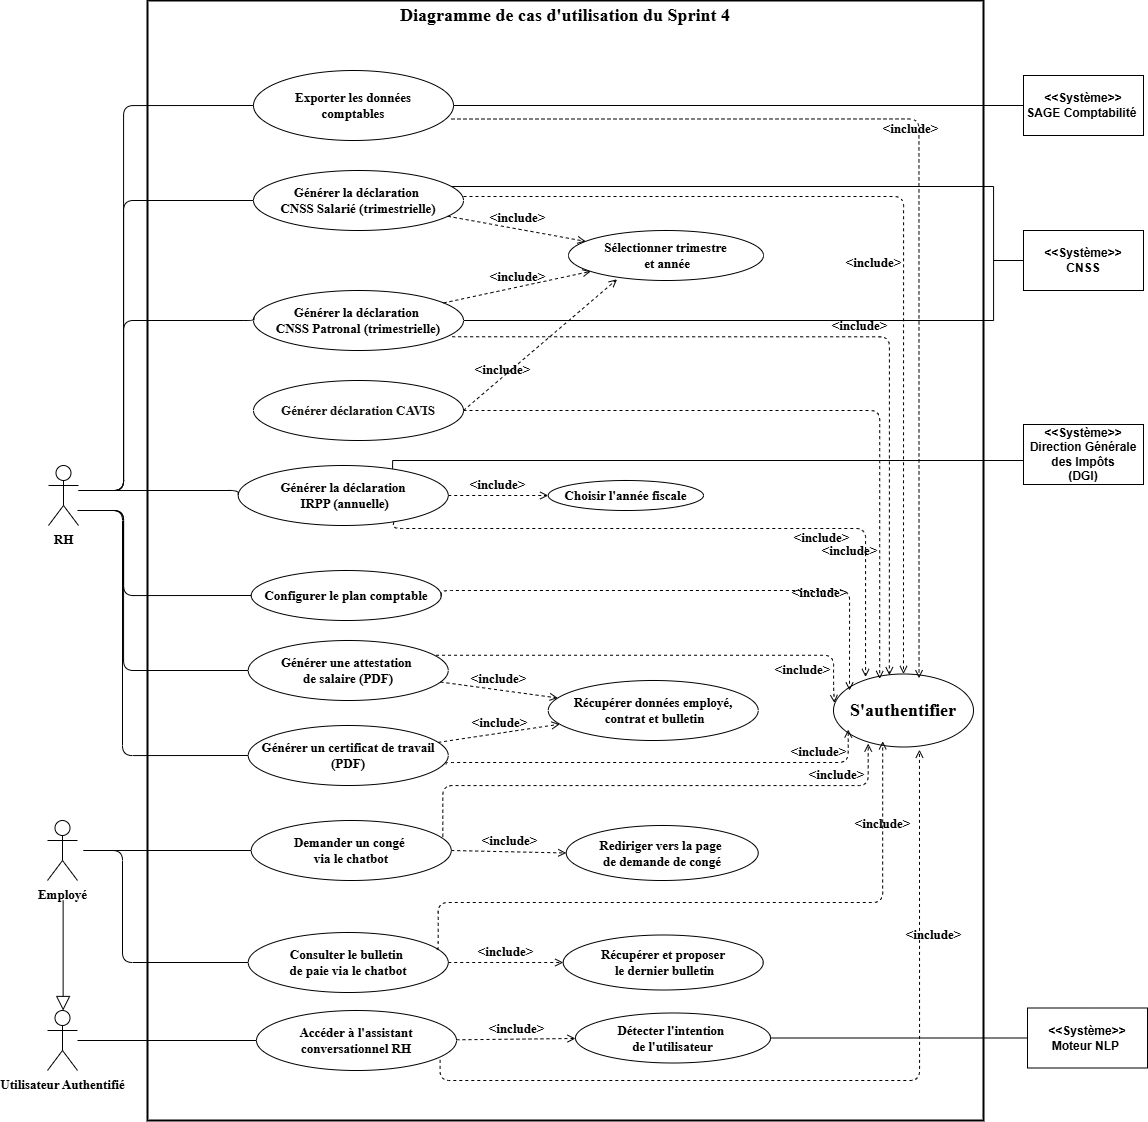
\includegraphics[width=0.95\textwidth]{use-case-sp4.png}
    \caption{Diagramme de cas d'utilisation du Sprint 4}
    \label{fig:use-case-sp4}
\end{figure}

% CORRECTION : Description UC enrichie avec relations UML et responsabilités par rôle précis
Le diagramme de cas d'utilisation du Sprint~4 (Figure~\ref{fig:use-case-sp4})
organise les fonctionnalités en quatre packages distincts, chacun
gouverné par des contraintes d'accès précises.

\textbf{Relations UML~:} Le cas d'utilisation «~Configurer le plan
comptable~» est en relation \texttt{<<include>>} avec
«~Exporter SAGE~», car l'export ne peut produire des écritures
cohérentes que si le plan est configuré. Les quatre actions de
génération de déclarations partagent une précondition commune
(\texttt{<<include>>} «~S'authentifier~» et «~Vérifier périodes
clôturées~»).

\textbf{Responsabilités par acteur~:}

\begin{itemize}[label=\textbullet, leftmargin=0.6cm]
    \item \textbf{Admin / RH Comptable~:}
          Configurer et exporter le plan comptable (CRUD +
          export SAGE). Générer les quatre déclarations
          réglementaires (CNSS salarié/patronal, CAVIS, IRPP).
          Produire les documents officiels (attestations de salaire,
          certificats de travail). Interroger les données RH
          de la société via l'intention \texttt{ADMIN\_SQL}
          du chatbot (effectif, masse salariale, statistiques).

    \item \textbf{Employé~:}
          Accéder au chatbot pour consulter ses données personnelles
          (\texttt{PERSONAL\_SQL}~: salaire, solde de congés,
          ancienneté, poste), initier une demande de congé
          (redirection) et poser des questions réglementaires
          (\texttt{LEGAL\_RAG}~: CNSS, IRPP, code du travail).

    \item \textbf{Utilisateur (tous rôles)~:}
          Accéder aux réponses conversationnelles générales
          (\texttt{GENERAL}~: salutations, questions RH génériques).
\end{itemize}

% -----------------------------------------------------------
\subsection{Description textuelle des cas d'utilisation}
% -----------------------------------------------------------

Les descriptions textuelles suivantes formalisent les préconditions,
scénarios nominaux et alternatifs des cas d'utilisation les plus
critiques du Sprint 4. Elles constituent la référence contractuelle
de validation avec le Product Owner.

% -----------------------------------------------------------
\subsubsection{Cas d'utilisation : Générer les déclarations de conformité réglementaire}
% -----------------------------------------------------------

Le tableau~\ref{tab:cu-conformite} présente la description textuelle
détaillée du cas d'utilisation « Générer les déclarations de conformité
réglementaire ».
\mbox{}\\

\begin{xltabular}{\textwidth}{|l|X|}
\caption{Description textuelle du cas d'utilisation Générer les déclarations de conformité}
\label{tab:cu-conformite} \\
\hline
\rowcolor[gray]{0.9} \textbf{Élément} & \textbf{Description} \\ \hline
\endfirsthead
\hline
\endlastfoot
\textbf{Titre} & Générer les déclarations de conformité réglementaire (CNSS / CAVIS / IRPP) \\ \hline
\textbf{Acteur principal} & RH \\ \hline
\textbf{Préconditions} & Des périodes de paie clôturées (\texttt{LOCKED}) existent pour la période concernée. Les paramètres réglementaires (taux CNSS, CAVIS, barèmes IRPP) sont configurés. \\ \hline
\textbf{Postconditions} & Un fichier déclaratif (CSV ou PDF) est généré et mis à disposition du RH pour téléchargement. \\ \hline
\textbf{Scénario principal} &
\begin{enumerate}[nosep, leftmargin=*]
    \item Le RH accède à l'onglet « Conformité » de la plateforme.
    \item Il sélectionne le type de déclaration souhaitée (CNSS Salarié, CNSS Patronal, CAVIS ou IRPP).
    \item Pour les déclarations trimestrielles, il sélectionne le trimestre et l'année cibles.
    \item Pour la déclaration IRPP, il sélectionne l'exercice fiscal annuel.
    \item Le système agrège les montants correspondants depuis les bulletins clôturés.
    \item Il génère le fichier déclaratif au format réglementaire.
    \item Le fichier est proposé en téléchargement au RH.
\end{enumerate} \\ \hline
\textbf{Scénarios alternatifs}
& \textbf{A1 : Aucune période clôturée} $\rightarrow$ Le système affiche un message indiquant l'absence de données et bloque la génération. \\ \cline{2-2}
& \textbf{A2 : Paramètres réglementaires manquants} $\rightarrow$ Le système lève une erreur bloquante invitant le Super Admin à configurer les taux. \\
\end{xltabular}

% -----------------------------------------------------------
\subsubsection{Cas d'utilisation : Interagir avec l'assistant conversationnel RH}
% -----------------------------------------------------------

Le tableau~\ref{tab:cu-chatbot} présente la description textuelle
détaillée du cas d'utilisation « Interagir avec l'assistant conversationnel RH ».
\mbox{}\\

\begin{xltabular}{\textwidth}{|l|X|}
\caption{Description textuelle du cas d'utilisation Interagir avec le chatbot RH}
\label{tab:cu-chatbot} \\
\hline
\rowcolor[gray]{0.9} \textbf{Élément} & \textbf{Description} \\ \hline
\endfirsthead
\hline
\endlastfoot
\textbf{Titre} & Interagir avec l'assistant conversationnel RH (PaieBot) \\ \hline
\textbf{Acteurs principaux} & Employé --- RH --- Admin \\ \hline
\textbf{Préconditions} & L'utilisateur est authentifié sur la plateforme PaieZone. \\ \hline
\textbf{Postconditions} & L'utilisateur obtient une réponse à sa question RH, est redirigé vers la fonctionnalité adéquate, ou reçoit des statistiques formatées. \\ \hline
\textbf{Scénario principal} &
    \begin{enumerate}[nosep, leftmargin=*]
        \item L'utilisateur clique sur le composant chatbot flottant visible après connexion.
        \item Il saisit sa question en langage naturel.
        \item Le système détecte l'intention parmi quatre catégories~: \texttt{PERSONAL\_SQL}, \texttt{ADMIN\_SQL}, \texttt{LEGAL\_RAG}, \texttt{GENERAL}.
        \item \textbf{Intention \texttt{PERSONAL\_SQL}} : Le pipeline génère une requête SQL sécurisée, l'exécute dans le schéma dédié et retourne le résultat formaté.
        \item \textbf{Intention \texttt{ADMIN\_SQL}} (Admin/RH uniquement) : Même pipeline avec droits élargis pour les statistiques de l'entreprise.
        \item \textbf{Intention \texttt{LEGAL\_RAG}} : Le pipeline RAG recherche dans \texttt{KnowledgeDocument} et génère une réponse contextualisée.
        \item \textbf{Intention \texttt{GENERAL}} : Réponse directe par phi3 en mode conversationnel.
    \end{enumerate} \\ \hline
\textbf{Scénarios alternatifs}
& \textbf{A1 : Intention non reconnue} $\rightarrow$ Le chatbot informe l'utilisateur et propose des exemples de questions reconnues. \\ \cline{2-2}
& \textbf{A2 : Tentative d'accès aux données d'un collègue} $\rightarrow$ Le système refuse avec message de confidentialité, aucune donnée exposée. \\ \cline{2-2}
& \textbf{A3 : SQL dangereux détecté} $\rightarrow$ La requête est rejetée par le validateur de sécurité. \\
\end{xltabular}

% ============================================================
\section{Conception du quatrième Sprint}
\label{sec:s4-conception}
% ============================================================

La conception technique du Sprint 4 traduit les besoins métiers en
modèles structurants guidant le développement. Cette section s'articule
autour de deux axes complémentaires~: le diagramme de classes, qui
modélise l'architecture statique des nouvelles entités, et les
diagrammes de séquence, qui illustrent les interactions dynamiques
entre les composants du système.

% -----------------------------------------------------------
\subsection{Diagramme de classes}
\label{sec:s4-classes}
% -----------------------------------------------------------

Le diagramme de classes du Sprint 4 complète le modèle établi lors du
Sprint 3 en introduisant les entités nécessaires à la comptabilité, à
la conformité, aux documents RH et à l'assistant conversationnel.
Il définit la structure des données ainsi que les relations qui les
unissent avec les entités existantes (\texttt{PayrollPeriod},
\texttt{PaySlip}, \texttt{Employee}, \texttt{Contract}).

La figure~\ref{fig:classes-sprint4} présente le diagramme de classes
du Sprint 4, illustrant l'extension finale du modèle de données de
PaieZone.

\newpage
\begin{figure}[H]
    \vspace*{-0.18cm}
    \centering
    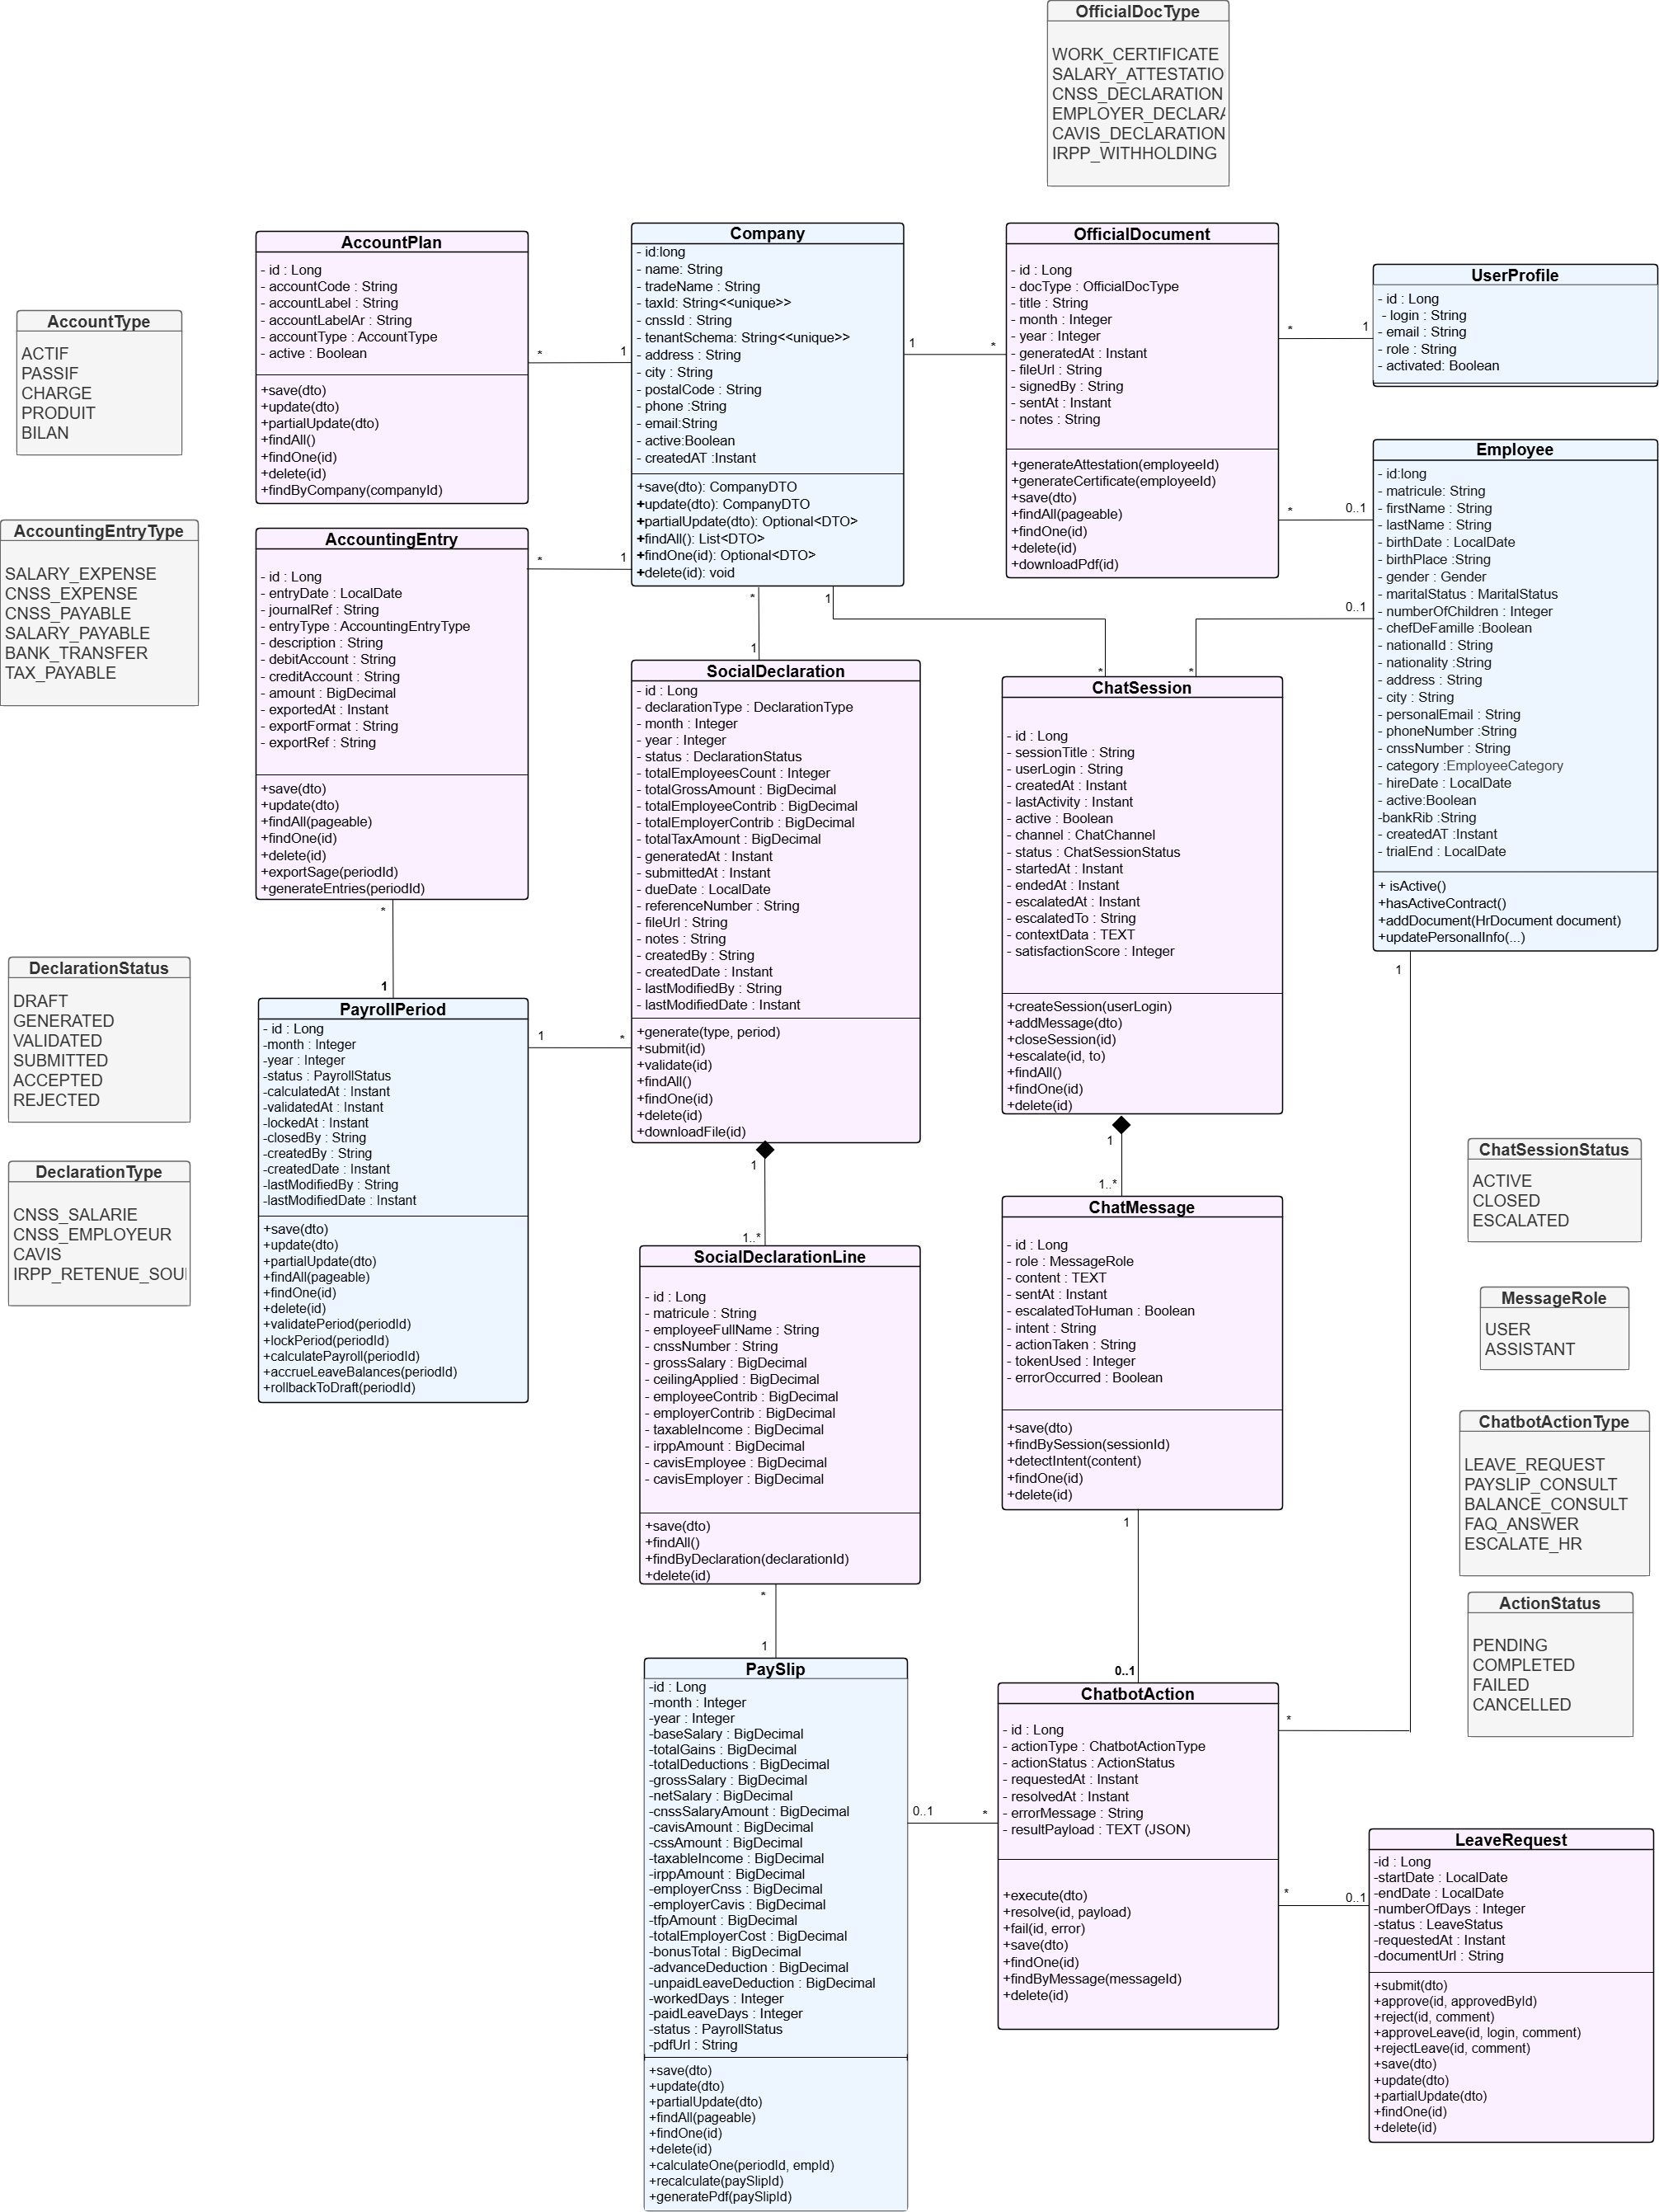
\includegraphics[width=0.95\textwidth]{classes-sprint4.png}
    \caption{Diagramme de classes du Sprint 4}
    \label{fig:classes-sprint4}
\end{figure}

% CORRECTION : Noms corrigés (PayrollPeriod, SocialDeclaration) + entités manquantes ajoutées
% (AccountingEntry, SocialDeclarationLine, ChatSession, ChatMessage, KnowledgeDocument)
Les entités principales introduites dans ce sprint sont les
suivantes~:

\begin{itemize}[label=\textbullet, leftmargin=0.6cm]

    \item \textbf{\texttt{AccountPlan}}~: modélise le plan comptable
          de la société. Chaque entrée associe un code de compte
          (\texttt{accountCode}), un libellé (\texttt{label}), un type
          (\texttt{accountType}) et optionnellement une rubrique de
          paie (\texttt{Rubrique}), permettant la génération de
          l'export comptable SAGE.

    \item \textbf{\texttt{AccountingEntry}}~: représente une écriture
          comptable individuelle générée depuis un bulletin de paie.
          Elle lie un \texttt{AccountPlan}, un \texttt{PaySlip} et
          enregistre le montant, le sens (débit/crédit) et le type
          de l'écriture (\texttt{AccountingEntryType}).

    \item \textbf{\texttt{SocialDeclaration}}~: conserve les données
          agrégées de chaque déclaration réglementaire générée
          (type~: CNSS\_SALARY, CNSS\_EMPLOYER, CAVIS, IRPP~;
          période de référence~; totaux salarié/patronal~; statut~;
          horodatage de génération~; URL du fichier produit).
          Liée à \texttt{Company} et \texttt{PayrollPeriod}.

    \item \textbf{\texttt{SocialDeclarationLine}}~: détail ligne
          par ligne de la déclaration, avec le montant individuel
          par employé, permettant la traçabilité des montants
          déclarés.

    \item \textbf{\texttt{OfficialDocument}}~: stocke les métadonnées
          des documents officiels générés automatiquement
          (attestations de salaire, certificats de travail,
          fichiers de déclaration)~; typé via \texttt{OfficialDocType}
          (WORK\_CERTIFICATE, SALARY\_ATTESTATION,
          CNSS\_DECLARATION, CAVIS\_DECLARATION,
          IRPP\_WITHHOLDING). Liée à \texttt{Employee}.

    \item \textbf{\texttt{ChatSession}}~: session de conversation
          PaieBot identifiée par \texttt{userLogin}. Porte le titre
          de la session (auto-généré depuis le premier message),
          les horodatages de création et de dernière activité,
          et le statut actif/fermé.

    \item \textbf{\texttt{ChatMessage}}~: message unitaire de la
          conversation. Stocke le rôle (\texttt{USER} ou
          \texttt{ASSISTANT}), le contenu, l'intention détectée
          (\texttt{IntentType}~: PERSONAL\_SQL, ADMIN\_SQL,
          LEGAL\_RAG, GENERAL) et un indicateur d'escalade vers
          le RH humain (\texttt{escalatedToHuman}).

    \item \textbf{\texttt{KnowledgeDocument}}~: base documentaire
          du système RAG. Chaque document porte un titre, un
          contenu textuel, une catégorie et des mots-clés indexés
          (\texttt{keywords}) utilisés pour la correspondance lors
          des requêtes \texttt{LEGAL\_RAG}.

\end{itemize}

% -----------------------------------------------------------
\subsection{Diagrammes de séquences}
% -----------------------------------------------------------

Les diagrammes de séquences illustrent la dynamique du système en
détaillant les interactions chronologiques entre les composants pour
les cas d'utilisation les plus critiques.

% -----------------------------------------------------------
\subsubsection{Diagramme de séquence : Générer une déclaration de conformité}
% -----------------------------------------------------------

La figure~\ref{fig:seq-conformite} illustre le flux de génération
d'une déclaration réglementaire (CNSS, CAVIS ou IRPP).

\begin{figure}[H]
    \vspace*{-0.18cm}
    \centering
    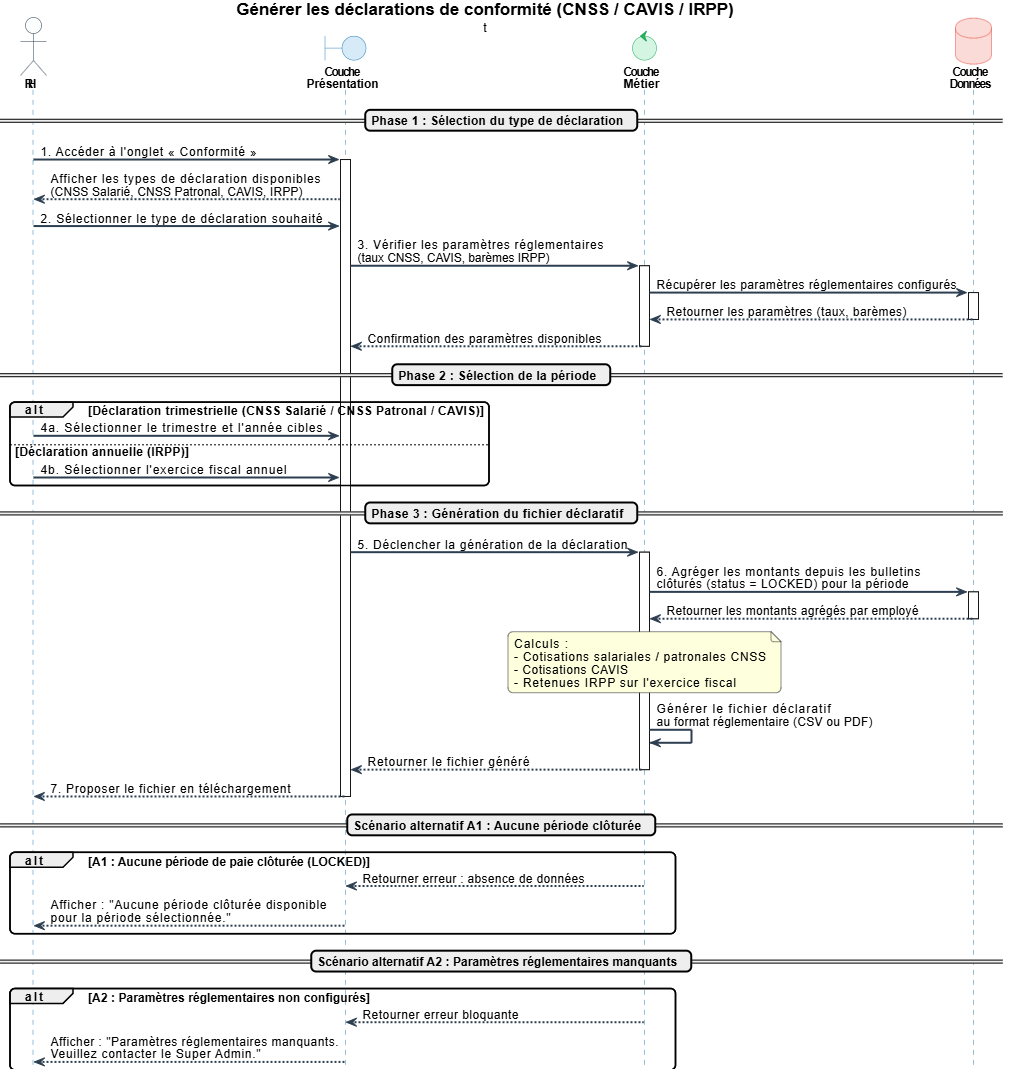
\includegraphics[width=0.85\textwidth]{seq-sp4-uc1.png}
    \caption{Diagramme de séquence --- Générer une déclaration de conformité}
    \label{fig:seq-conformite}
\end{figure}

Ce diagramme illustre l'agrégation automatique des données financières
issues des bulletins clôturés pour produire un fichier déclaratif
conforme aux exigences des organismes tunisiens~\cite{cnss_reg,lf2026}.
Le flux garantit l'intégrité des montants déclarés par rapport aux
données calculées lors du cycle de paie.

% -----------------------------------------------------------
\subsubsection{Diagramme de séquence : Interaction avec le chatbot RH}
% -----------------------------------------------------------

La figure~\ref{fig:seq-chatbot} illustre le flux d'interaction entre
un utilisateur et l'assistant conversationnel RH de PaieZone.

\begin{figure}[H]
    \vspace*{-0.18cm}
    \centering
    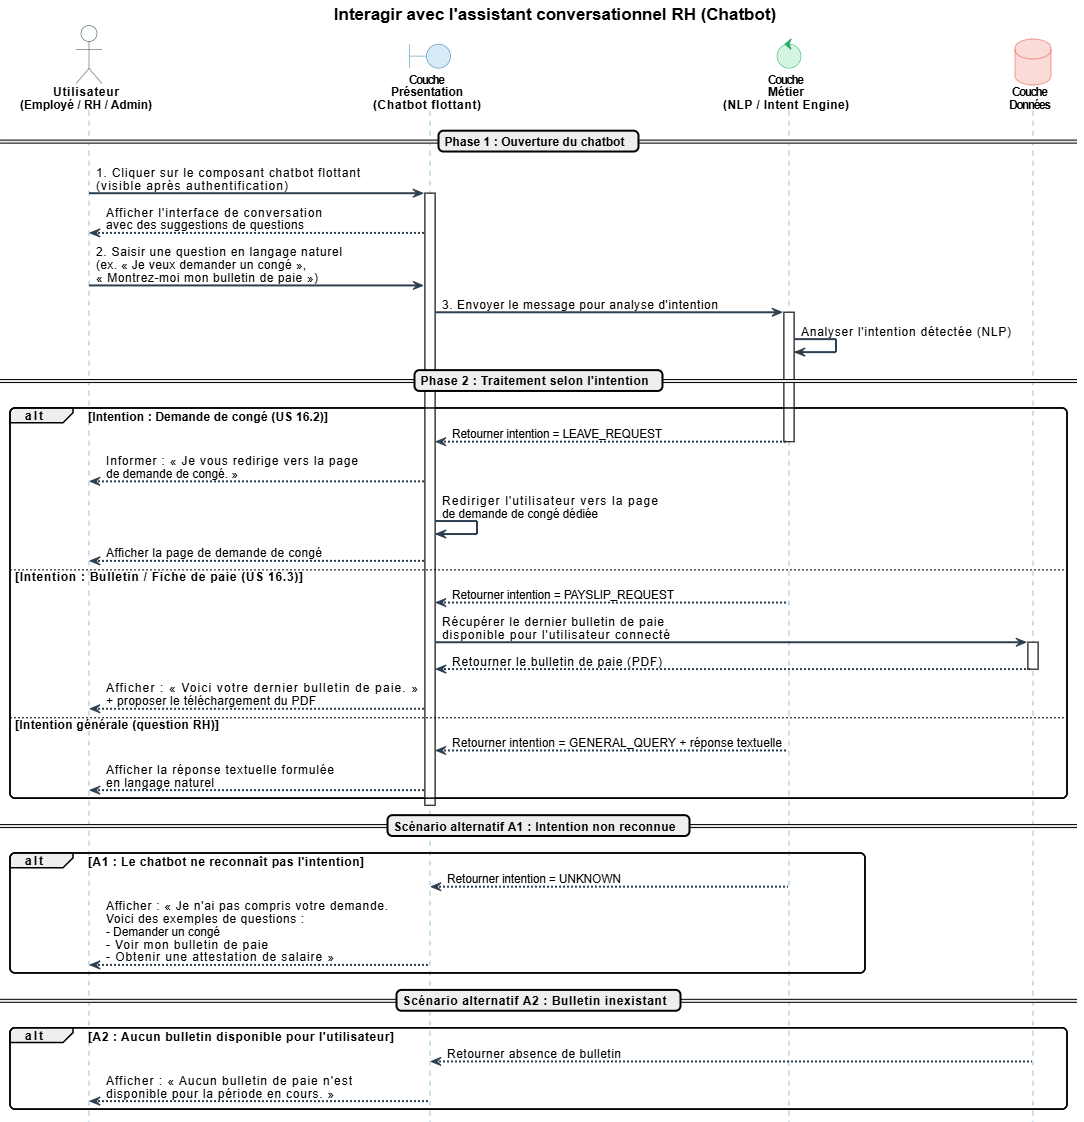
\includegraphics[width=0.80\textwidth]{seq-sp4-uc2.png}
    \caption{Diagramme de séquence --- Interaction avec le chatbot RH}
    \label{fig:seq-chatbot}
\end{figure}
\newpage

% CORRECTION : "détection légère des intentions" remplacé par description technique complète
Ce diagramme modélise le pipeline complet de traitement d'un message
utilisateur par PaieBot, l'assistant conversationnel de PaieZone~RH.

\textbf{Architecture à quatre intentions~:} À réception d'un message,
\texttt{TextToSqlService.detectIntent()} analyse le texte normalisé
et le classe parmi quatre catégories~:

\begin{itemize}[label=\textbullet, leftmargin=0.6cm]
    \item \textbf{\texttt{PERSONAL\_SQL}}~: questions de l'employé sur
          ses propres données (salaire, congés, ancienneté, poste).
          Le pipeline génère une requête SQL via Ollama~phi3
          (température 0,05 --- déterministe), la valide, l'exécute
          dans le schéma PostgreSQL~\cite{postgresql} du tenant, et formate le résultat
          en Markdown.

    \item \textbf{\texttt{ADMIN\_SQL}}~: questions RH/Admin sur les
          données de l'entreprise (effectif, masse salariale,
          répartition). Même pipeline SQL avec droits élargis
          (pas de filtre \texttt{user\_profile\_id}).

    \item \textbf{\texttt{LEGAL\_RAG}}~: questions réglementaires
          (CNSS, IRPP, code du travail, conventions collectives).
          Les documents \texttt{KnowledgeDocument} correspondant
          aux mots-clés de la question sont injectés dans le prompt
          système d'Ollama (RAG~\cite{rag}). La réponse est générée par phi3
          en mode conversationnel (température 0,7).

    \item \textbf{\texttt{GENERAL}}~: salutations et questions
          génériques traitées directement par phi3~\cite{phi3} sans base de
          connaissances.
\end{itemize}

\textbf{Garanties de sécurité~:} Avant tout traitement, le système
vérifie qu'un employé n'essaie pas d'accéder aux données d'un
collègue (protection inter-tenant). Les requêtes SQL générées
sont systématiquement validées (blocage de DROP, DELETE, ALTER,
TRUNCATE, etc.) et exécutées avec \texttt{SET search\_path} pour
l'isolation multi-tenant. Les réponses contenant des hallucinations
caractéristiques de phi3 sont détectées par analyse regex et
remplacées par un message d'erreur générique.

% ============================================================
\section{Étude et réalisation du quatrième sprint}
\label{sec:s4-realisation}
% ============================================================

Cette section présente les réalisations concrètes du Sprint 4, marquant
la finalisation de la plateforme PaieZone. Les travaux ont porté sur
l'implémentation du module comptable, la génération des déclarations
réglementaires, la production automatisée des documents administratifs
RH et le déploiement de l'assistant conversationnel PaieBot.

% ============================================================
\subsection{Gestion comptable et export SAGE}
% ============================================================

\begin{figure}[H]
    \vspace*{-0.18cm}
    \centering
    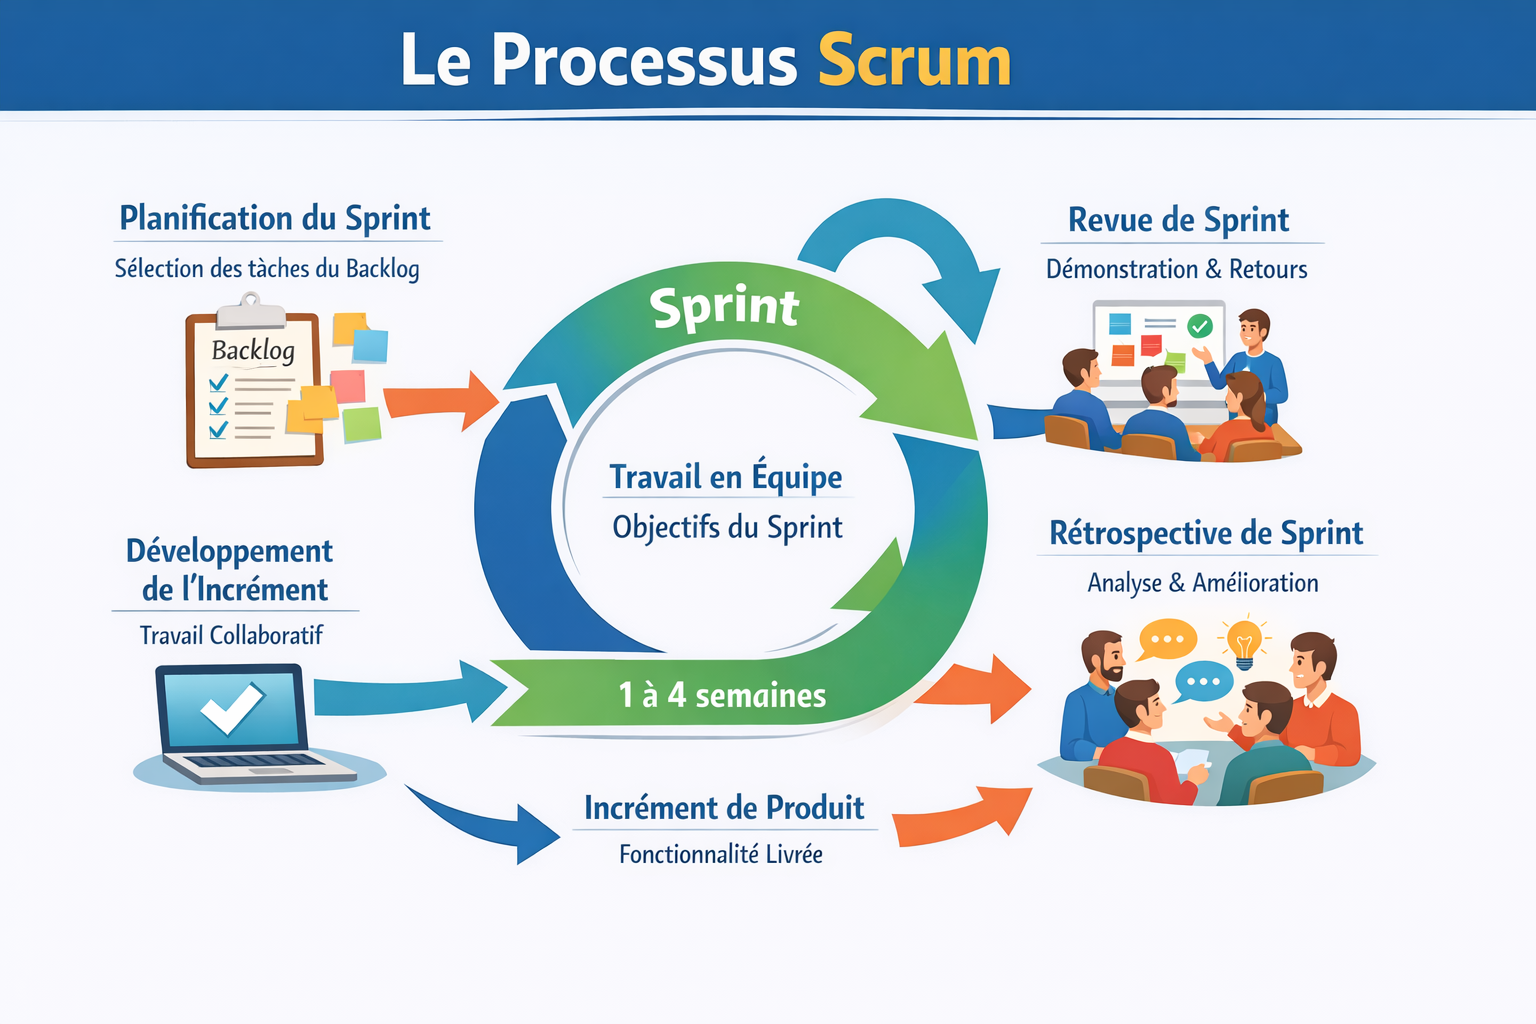
\includegraphics[width=0.70\textwidth]{scrum.png}
    \caption{Interface de gestion du plan comptable et export SAGE}
    \label{fig:ui-comptabilite}
\end{figure}

La figure~\ref{fig:ui-comptabilite} présente l'interface de l'onglet
Comptabilité de PaieZone. Le RH ou l'Administrateur dispose d'un
tableau de gestion du plan comptable offrant un CRUD complet (création,
modification, suppression de comptes). Un bouton « Exporter SAGE (.csv) »
permet de générer à la demande un fichier d'export conforme au format
attendu par les logiciels comptables SAGE, contenant les écritures
issues des bulletins de paie clôturés.

% ============================================================
\subsection{Conformité réglementaire}
% ============================================================

\begin{figure}[H]
    \vspace*{-0.18cm}
    \centering
    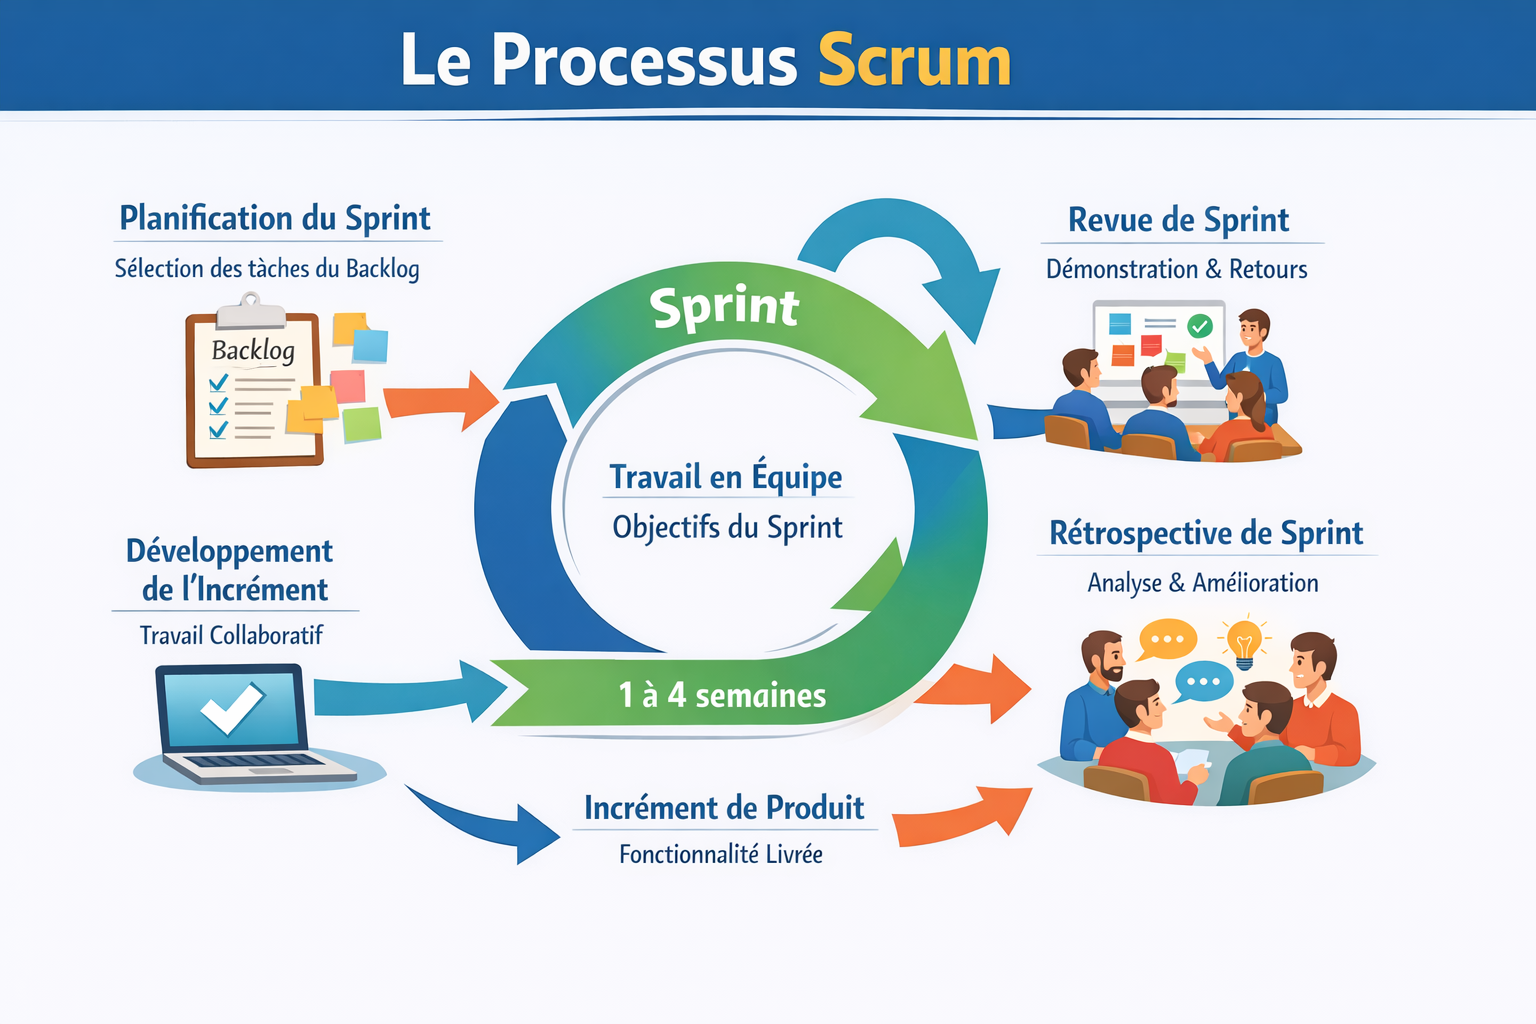
\includegraphics[width=0.70\textwidth]{scrum.png}
    \caption{Interface de l'onglet Conformité --- Déclarations CNSS, CAVIS et IRPP}
    \label{fig:ui-conformite}
\end{figure}

La figure~\ref{fig:ui-conformite} présente le module de conformité
réglementaire. Le RH accède à quatre actions de génération~:
déclaration CNSS salarié, déclaration CNSS patronal, déclaration
CAVIS (toutes trois au pas trimestriel) et déclaration IRPP
(annuelle). Chaque déclenchement agrège automatiquement les montants
depuis les bulletins clôturés de la période sélectionnée et produit
un fichier téléchargeable conforme aux exigences légales
tunisiennes~\cite{loifinance,cnss_reg}.

% ============================================================
\subsection{Documents administratifs RH}
% ============================================================

\begin{figure}[H]
    \vspace*{-0.18cm}
    \centering
    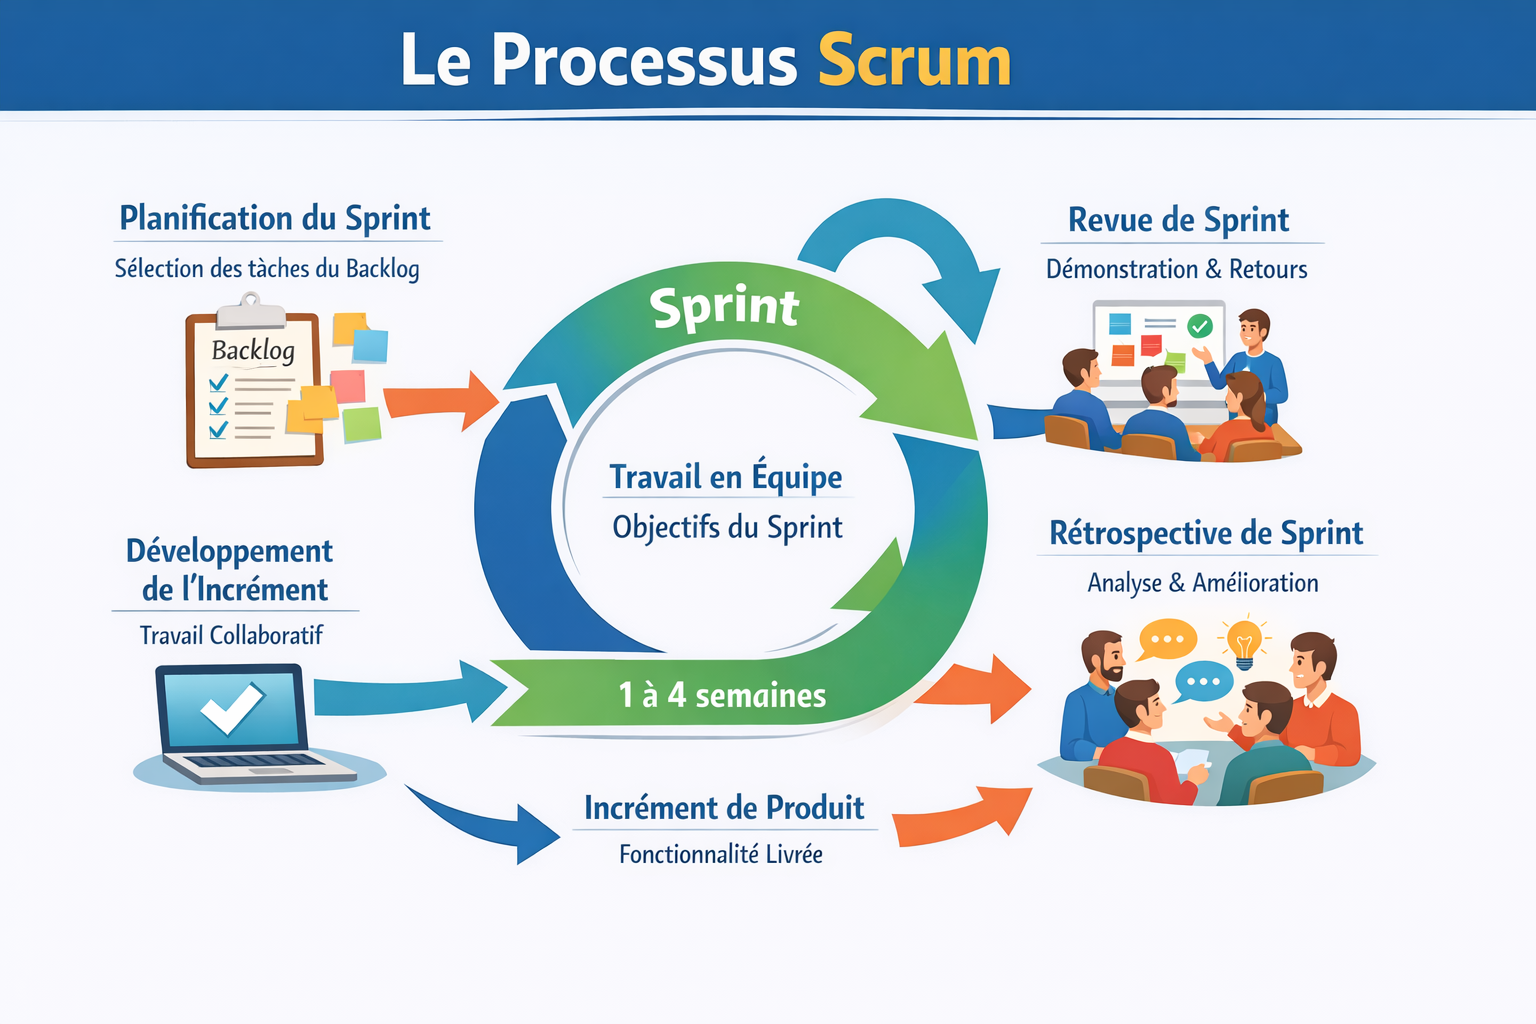
\includegraphics[width=0.70\textwidth]{scrum.png}
    \caption{Génération de l'attestation de salaire et du certificat de travail}
    \label{fig:ui-docs-rh}
\end{figure}

La figure~\ref{fig:ui-docs-rh} illustre la fonctionnalité de génération
des documents administratifs RH accessible depuis la page Employés.
Un clic sur le bouton de téléchargement PDF déclenche la génération
de l'attestation de salaire ou du certificat de travail via le moteur
\textbf{Flying Saucer}~\cite{flyingsaucer} (\texttt{ITextRenderer}),
directement alimentés par les données du dossier employé et de son
dernier bulletin calculé. Les documents respectent les templates
légaux en vigueur et sont disponibles immédiatement en téléchargement.

% ============================================================
\subsection{Assistant conversationnel RH (PaieBot)}
\label{sec:s4-chatbot}
% ============================================================

\begin{figure}[H]
    \vspace*{-0.18cm}
    \centering
    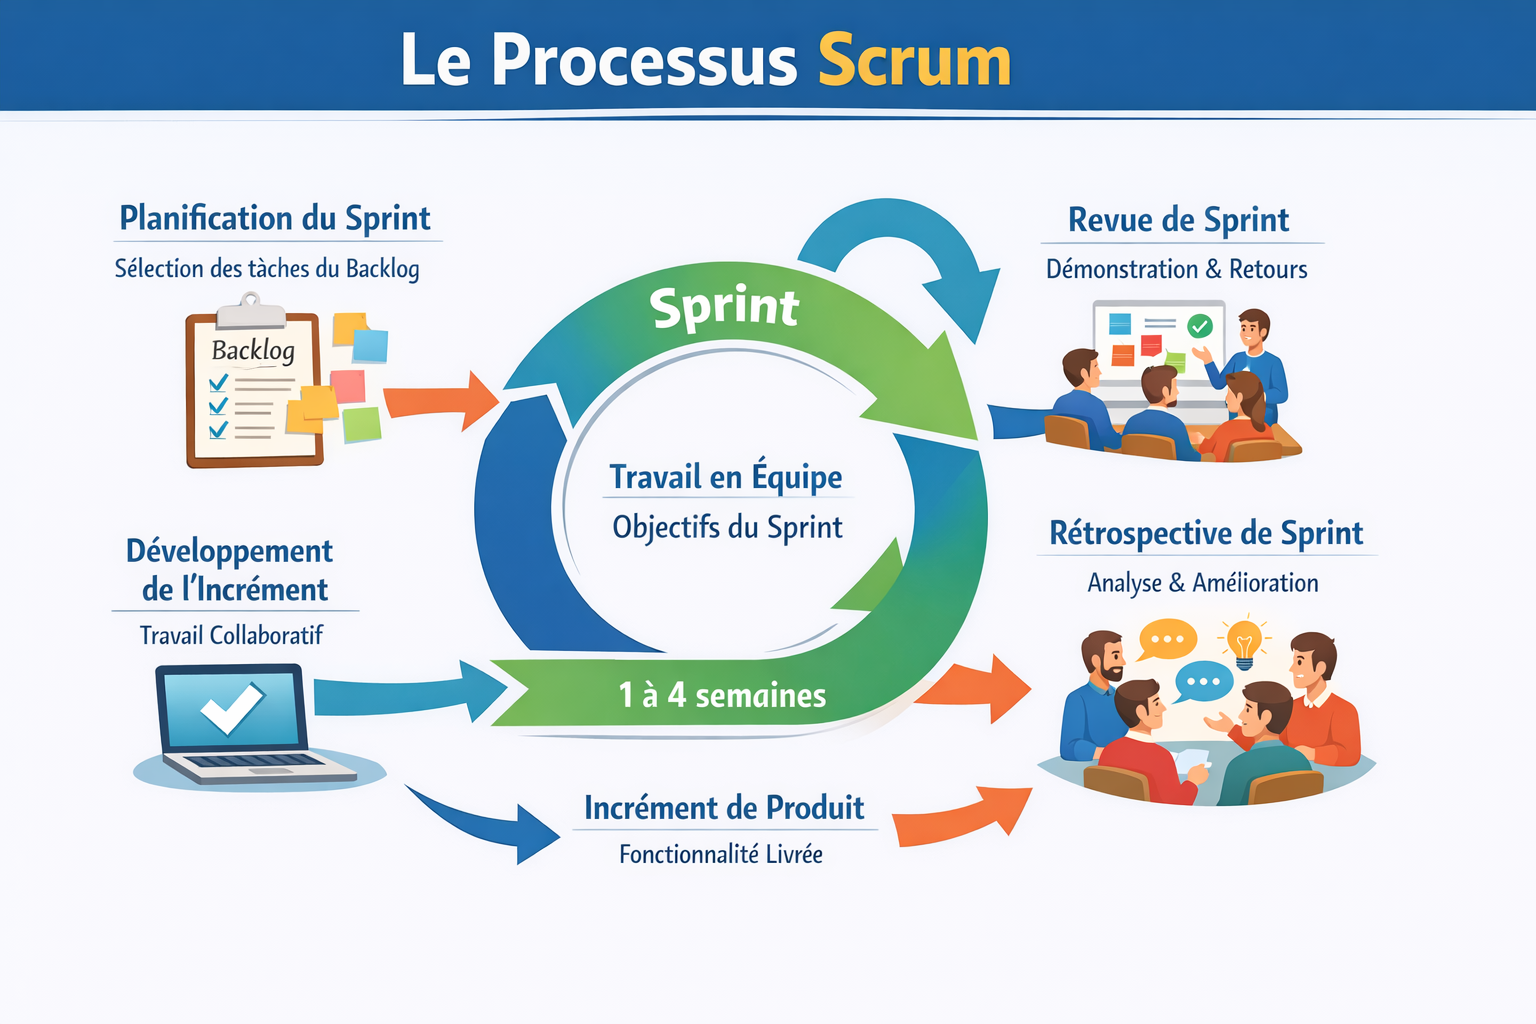
\includegraphics[width=0.70\textwidth]{scrum.png}
    \caption{Composant PaieBot --- Assistant conversationnel RH flottant}
    \label{fig:ui-chatbot}
\end{figure}

% CORRECTION : Description complète des 4 intentions + mécanismes de sécurité
La figure~\ref{fig:ui-chatbot} présente le composant chatbot flottant
PaieBot de PaieZone~RH, visible par tous les utilisateurs après
authentification. L'assistant traite quatre catégories de requêtes~:

\begin{itemize}[label=\textbullet, leftmargin=0.6cm]
    \item \textbf{Données personnelles (\texttt{PERSONAL\_SQL})~:}
          L'employé peut interroger ses propres informations en langage
          naturel («~Quel est mon salaire net~?~», «~Combien de jours de
          congé me restent~?~», «~Quel est mon poste~?~»). Le système
          génère une requête SQL sécurisée, l'exécute dans le schéma
          dédié et retourne le résultat formaté.

    \item \textbf{Statistiques RH (\texttt{ADMIN\_SQL})~:}
          Pour les rôles Admin et RH uniquement, PaieBot peut répondre
          à des questions agrégées («~Combien d'employés actifs~?~»,
          «~Quelle est la masse salariale~?~», «~Effectif par
          département~?~»).

    \item \textbf{Réglementation (\texttt{LEGAL\_RAG})~:}
          Les questions sur le code du travail tunisien, les taux CNSS
          et IRPP, les conventions collectives ou les congés légaux
          sont traitées par le pipeline RAG~\cite{rag}~: recherche dans la base
          documentaire (\texttt{KnowledgeDocument}) et génération d'une
          réponse contextualisée par le modèle phi3~\cite{phi3}.

    \item \textbf{Général (\texttt{GENERAL})~:}
          Salutations et questions courtes traitées directement par
          phi3~\cite{phi3} en mode conversationnel.
\end{itemize}

Les mécanismes de sécurité implémentés garantissent~: l'isolation
des données par tenant, le blocage des requêtes inter-employés,
la détection et la suppression des hallucinations du modèle,
et l'escalade automatique vers le service RH pour les situations
d'urgence détectées.

% ============================================================
\section{Tests et Validation}
\label{sec:s4-tests}
% ============================================================

La phase de tests et de validation du Sprint 4 vise à garantir la
conformité des fichiers déclaratifs produits et la fiabilité de
l'assistant conversationnel. Trois niveaux de tests ont été mis en
œuvre de manière complémentaire.

% -----------------------------------------------------------
\subsection{Plan de tests}
% -----------------------------------------------------------

\begin{itemize}[label=\textbullet, leftmargin=0.6cm]
    \item \textbf{Tests unitaires (JUnit~5, Mockito)} : Validation des
    services de génération --- notamment les algorithmes d'agrégation
    des montants CNSS, CAVIS et IRPP, et la cohérence des écritures
    comptables produites.
    \item \textbf{Tests d'intégration} : Validation des flux complets ---
    génération des déclarations sur des périodes clôturées réelles,
    export SAGE et vérification des montants par rapprochement avec
    les bulletins sources.
    \item \textbf{Tests fonctionnels (interface Angular~\cite{angular})} : Vérification
    du comportement des formulaires, de la conformité des PDF générés,
    et de la robustesse du chatbot face aux quatre intentions et aux
    cas limites de sécurité.
\end{itemize}

\vspace{0.4cm}
% CORRECTION : Tableau renommé 6.6 (éviter duplication avec Table 6.2 du Backlog)
% + Tests chatbot enrichis : PERSONAL_SQL, LEGAL_RAG, sécurité inter-tenant, SQL dangereux
Le Tableau~\ref{tab:tests-sprint4-recap} synthétise les cas de test principaux
réalisés pour ce sprint.

\renewcommand{\arraystretch}{1.3}
\begin{longtable}{|c|p{7.5cm}|p{4.5cm}|c|}
\caption{Récapitulatif des cas de test du Sprint~4}
\label{tab:tests-sprint4-recap} \\
\hline
\textbf{ID Test} &
\textbf{Description du cas de test} &
\textbf{Résultat attendu} &
\textbf{Statut} \\
\hline
\endfirsthead
\hline
\textbf{ID Test} &
\textbf{Description du cas de test} &
\textbf{Résultat attendu} &
\textbf{Statut} \\
\hline
\endhead
\hline
\endfoot
\hline
\endlastfoot

T-13.1 & CRUD complet du plan comptable & Opérations sans erreur, données persistées & \textcolor{green!60!black}{\textbf{OK}} \\ \hline
T-13.2 & Export SAGE sur une période clôturée & Fichier CSV conforme au format SAGE, téléchargeable & \textcolor{green!60!black}{\textbf{OK}} \\ \hline
T-14.1 & Génération CNSS salarié pour un trimestre avec 5 employés & Montants cohérents avec les bulletins calculés & \textcolor{green!60!black}{\textbf{OK}} \\ \hline
T-14.2 & Génération CNSS patronal trimestrielle & Montants patronaux conformes aux taux configurés & \textcolor{green!60!black}{\textbf{OK}} \\ \hline
T-14.3 & Génération CAVIS trimestrielle & Fichier CAVIS conforme aux exigences légales & \textcolor{green!60!black}{\textbf{OK}} \\ \hline
T-14.4 & Génération IRPP annuelle sur un exercice complet & État récapitulatif IRPP conforme aux exigences DGI & \textcolor{green!60!black}{\textbf{OK}} \\ \hline
T-14.5 & Génération d'une déclaration sans période clôturée & Erreur bloquante, aucun fichier généré & \textcolor{green!60!black}{\textbf{OK}} \\ \hline
T-15.1 & Génération de l'attestation de salaire PDF & PDF conforme au template avec données correctes & \textcolor{green!60!black}{\textbf{OK}} \\ \hline
T-15.2 & Génération du certificat de travail PDF & PDF avec données contractuelles exactes & \textcolor{green!60!black}{\textbf{OK}} \\ \hline
T-16.1 & Affichage du composant chatbot après authentification (tous rôles) & Composant flottant visible pour tous les rôles & \textcolor{green!60!black}{\textbf{OK}} \\ \hline
T-16.2 & Intention \texttt{PERSONAL\_SQL}~: «~Quel est mon salaire net~?~» & Résultat SQL formaté avec le salaire net de l'employé connecté & \textcolor{green!60!black}{\textbf{OK}} \\ \hline
T-16.3 & Intention \texttt{ADMIN\_SQL} (rôle RH)~: «~Effectif par département~» & Tableau Markdown avec les données de l'entreprise du tenant & \textcolor{green!60!black}{\textbf{OK}} \\ \hline
T-16.4 & Intention \texttt{LEGAL\_RAG}~: question sur le taux CNSS & Réponse basée sur \texttt{KnowledgeDocument}, conforme à la LF 2026 & \textcolor{green!60!black}{\textbf{OK}} \\ \hline
T-16.5 & Tentative d'accès aux données d'un autre employé & Refus avec message de confidentialité, aucune donnée exposée & \textcolor{green!60!black}{\textbf{OK}} \\ \hline
T-16.6 & Intention «~congé~» --- redirection & Redirection vers la page \texttt{/paiezone/emp-leaves} & \textcolor{green!60!black}{\textbf{OK}} \\ \hline
T-16.7 & SQL dangereux injecté dans la question (\texttt{DROP TABLE}) & Requête rejetée par le validateur de sécurité, message d'erreur & \textcolor{green!60!black}{\textbf{OK}} \\ \hline

\end{longtable}
\renewcommand{\arraystretch}{1.0}

% -----------------------------------------------------------
\subsection{Tests automatisés}
% -----------------------------------------------------------

Le Sprint~4 couvre les fonctionnalités les plus avancées de \pz{}~:
l'assistant conversationnel IA et les conventions sectorielles. Deux
risques critiques ont motivé une couverture de tests approfondie~:
la fuite d'informations cross-tenant via le chatbot et les
hallucinations du modèle phi3.

\paragraph{ChatbotServiceTest --- 13 cas de test (JUnit~5 + Mockito)}

\renewcommand{\arraystretch}{1.2}
\begin{small}
\begin{longtable}{|c|p{5.5cm}|p{3.8cm}|c|}
\hline
\rowcolor[gray]{0.9}
\textbf{ID} & \textbf{Scénario} & \textbf{Résultat attendu} & \textbf{Statut} \\ \hline
\endfirsthead \hline
\rowcolor[gray]{0.9}
\textbf{ID} & \textbf{Scénario} & \textbf{Résultat attendu} & \textbf{Statut} \\ \hline
\endhead \hline \endfoot \hline
\caption{Tests automatisés --- ChatbotServiceTest}\label{tab:auto-chatbot}\endlastfoot
TA-S4-01 & Création de session avec titre
    & DTO retourné, sauvegarde en base & \textcolor{green!60!black}{\textbf{OK}} \\ \hline
TA-S4-02 & Création de session sans titre
    & Titre = «~Nouvelle conversation~» & \textcolor{green!60!black}{\textbf{OK}} \\ \hline
TA-S4-03 & Accès à une session inexistante
    & HTTP 404 & \textcolor{green!60!black}{\textbf{OK}} \\ \hline
TA-S4-04 & Accès à la session d'un autre utilisateur
    & HTTP 404 (sécurité par obscurité) & \textcolor{green!60!black}{\textbf{OK}} \\ \hline
TA-S4-05 & Employé demande le salaire d'un collègue
    & Refus immédiat, Ollama non appelé & \textcolor{green!60!black}{\textbf{OK}} \\ \hline
TA-S4-06 & Admin envoie la même requête cross-tenant
    & Accès accordé, réponse retournée & \textcolor{green!60!black}{\textbf{OK}} \\ \hline
TA-S4-07 & Réponse phi3 contenant un email inventé
    & Email remplacé par message sûr & \textcolor{green!60!black}{\textbf{OK}} \\ \hline
TA-S4-08 & Réponse phi3 avec «~I'm sorry, but I cannot~»
    & Réponse remplacée & \textcolor{green!60!black}{\textbf{OK}} \\ \hline
TA-S4-09 & Réponse légitime phi3
    & Réponse conservée sans modification & \textcolor{green!60!black}{\textbf{OK}} \\ \hline
TA-S4-10 & Intention \texttt{ADMIN\_SQL} par un employé
    & Reclassifiée en \texttt{LEGAL\_RAG} & \textcolor{green!60!black}{\textbf{OK}} \\ \hline
TA-S4-11 & Intention \texttt{ADMIN\_SQL} par un RH Comptable
    & SQL exécuté, résultat retourné & \textcolor{green!60!black}{\textbf{OK}} \\ \hline
TA-S4-12 & Réponse contenant \texttt{[ESCALADE\_RH]}
    & \texttt{escalatedToHuman = true} & \textcolor{green!60!black}{\textbf{OK}} \\ \hline
TA-S4-13 & Tests E2E Cypress~: ouverture PaieBot, envoi message
    & Bulle utilisateur visible, réponse bot reçue & \textcolor{green!60!black}{\textbf{OK}} \\ \hline
\end{longtable}
\end{small}
\renewcommand{\arraystretch}{1.0}

\paragraph{Bug détecté et corrigé lors des tests}
L'écriture du test TA-S4-07 a révélé une anomalie~: le Signal Angular
\texttt{companiesLoaded} du \texttt{DataService} était positionné à
\texttt{true} même en cas d'erreur HTTP~500 sur l'endpoint
\texttt{/api/companies}, rendant le dashboard SaaS silencieusement vide.
Un nouveau Signal \texttt{companiesError} a été ajouté au
\texttt{DataService} et un mécanisme de retry a été intégré dans le
\texttt{SaasDashboardComponent}, garantissant que les données s'affichent
correctement après une erreur réseau transitoire.

\textbf{Résultat global Sprint~4~:} 13/13 tests automatisés passés
(\textcolor{green!60!black}{\textbf{OK}}), couverture estimée à
\textbf{72\,\%} pour \texttt{ChatbotService}.

% ============================================================
\section{Rituels Agiles et Clôture du Sprint}
\label{sec:s4-rituels}
% ============================================================

Conformément à la méthodologie Scrum~\cite{scrumguide} adoptée par l'équipe PaieZone,
le Sprint 4 s'est clôturé par la tenue des deux rituels essentiels~:
la Sprint Review et la Sprint Retrospective. Ces cérémonies assurent
la transparence du travail accompli et l'amélioration continue des
pratiques d'équipe.

% ============================================================
\subsection{Revue du Sprint (Sprint Review)}
% ============================================================

La Sprint Review a réuni l'équipe de développement, le Product Owner
et les parties prenantes. Les User Stories du sprint ont été présentées
et démontrées en conditions réelles à travers l'interface Angular~\cite{angular}~:

\begin{itemize}[label=\textbullet, leftmargin=0.6cm]
    \item \textbf{Module comptable :} Démonstration du plan comptable
    configurable et de l'export SAGE fonctionnel, validés sur un jeu de
    données représentatif.
    \item \textbf{Conformité réglementaire :} Présentation des quatre
    déclarations générées (CNSS salarié, CNSS patronal, CAVIS, IRPP),
    avec vérification des montants par rapport aux bulletins sources~\cite{cnss_reg,lf2026}.
    \item \textbf{Documents administratifs RH :} Validation des templates
    PDF de l'attestation de salaire et du certificat de travail,
    conformes aux exigences légales tunisiennes~\cite{flyingsaucer}.
    \item \textbf{Assistant conversationnel PaieBot :} Démonstration des
    quatre intentions (\texttt{PERSONAL\_SQL}, \texttt{ADMIN\_SQL},
    \texttt{LEGAL\_RAG}, \texttt{GENERAL}) et des mécanismes de
    sécurité (protection inter-tenant, validation SQL, anti-hallucination).
\end{itemize}

L'ensemble des User Stories planifiées pour ce quatrième sprint a été
validé par le Product Owner, confirmant la conformité des livrables
aux critères d'acceptation et clôturant ainsi le développement
fonctionnel de PaieZone.

% ============================================================
\subsection{Rétrospective du Sprint (Sprint Retrospective)}
% ============================================================

La Sprint Retrospective a permis à l'équipe de réfléchir collectivement
sur les pratiques du sprint écoulé autour de trois axes~:

\begin{itemize}[label=\textbullet, leftmargin=0.6cm]
    \item \textbf{Ce qui a bien fonctionné :} La réutilisation du service
    de génération PDF Flying Saucer~\cite{flyingsaucer} du Sprint 3 pour les attestations
    et certificats, qui a considérablement accéléré le développement.
    La modularité du pipeline d'intentions de PaieBot, dont l'architecture
    à quatre catégories permet d'ajouter de nouvelles capacités sans
    modifier le cœur du moteur de détection.
    \item \textbf{Ce qui peut être amélioré :} La mise en conformité des
    fichiers CNSS et CAVIS a nécessité plusieurs cycles de révision pour
    respecter précisément le format attendu par les organismes tunisiens.
    L'intégration d'Ollama/phi3~\cite{ollama,phi3} en local a demandé une
    configuration spécifique de l'environnement de déploiement.
    \item \textbf{Actions pour les projets futurs :} Intégrer des jeux
    de données de référence issus des organismes réglementaires dès la
    phase de spécification. Enrichir le chatbot pour permettre la création
    directe de demandes de congé depuis l'interface conversationnelle.
    Constituer une bibliothèque de formats d'export standardisés pour les
    outils comptables courants (SAGE, Ciel).
\end{itemize}

% ============================================================
\section*{Conclusion}
\label{sec:s4-conclusion}
\addcontentsline{toc}{section}{Conclusion}
% ============================================================

% CORRECTION : Conclusion enrichie pour valoriser l'innovation IA
Ce sixième chapitre a détaillé les réalisations du Sprint~4 de
PaieZone~RH, sprint conclusif couvrant onze User Stories et quatre
domaines complémentaires.

\textbf{Comptabilité et conformité~:} Le module de plan comptable
configurable, couplé à l'export SAGE automatisé, et les quatre
services de génération de déclarations (CNSS salarié/patronal,
CAVIS, IRPP) matérialisent la conformité totale de PaieZone au
cadre légal et fiscal tunisien --- de la Loi de Finances~2026~\cite{lf2026}
jusqu'aux formats déclaratifs des organismes sociaux~\cite{cnss_reg}.

\textbf{Documents officiels~:} La génération automatisée des
attestations de salaire et certificats de travail, via le moteur
PDF Flying Saucer~\cite{flyingsaucer}, élimine les tâches manuelles chronophages du
service RH et garantit la conformité aux templates légaux en vigueur.

\textbf{Innovation IA~:} L'assistant conversationnel PaieBot
représente la fonctionnalité différenciante de la plateforme.
Reposant sur le modèle de langage Ollama/phi3~\cite{ollama,phi3} déployé localement,
il intègre un pipeline Text-to-SQL sécurisé multi-tenant pour les
requêtes sur données structurées, une architecture RAG~\cite{rag} sur base
documentaire pour les questions réglementaires, et des mécanismes
de sécurité robustes (protection inter-tenant, anti-hallucination,
validation SQL). Aucune donnée RH ne transite vers des services
cloud tiers.

PaieZone~RH s'affirme ainsi comme une solution SaaS multi-tenant
complète et conforme, couvrant l'intégralité du cycle RH~:
du recrutement et de la gestion contractuelle jusqu'à la
déclaration réglementaire, l'export comptable et l'assistance
conversationnelle intelligente --- répondant aux exigences
du droit social tunisien et aux standards modernes d'une
plateforme RH~SaaS.

% ==========================================
% BIBLIOGRAPHIE COMPLÈTE
% ==========================================
% CORRECTION : Bibliographie complète avec références manquantes (Ollama, phi3, RAG, Flying Saucer)
% et URL Spring Boot versionnée + subsections organisées

\begin{thebibliography}{99}

\subsection*{Références Méthodologiques}

\bibitem{scrumguide}
  K.~Schwaber et J.~Sutherland.
  \emph{Le Guide Scrum~: Les règles du jeu}.
  \url{https://scrumguides.org}, 2020.

\bibitem{uml}
  G.~Booch, J.~Rumbaugh et I.~Jacobson.
  \emph{UML~: Guide de l'utilisateur}.
  Addison-Wesley, 2\textsuperscript{ème} édition, 2004.

\subsection*{Technologies Backend et Base de données}

\bibitem{springboot}
  Spring~IO.
  \emph{Spring Boot~4.0 Reference Documentation}.
  \url{https://docs.spring.io/spring-boot/docs/4.0.x/reference/html/},
  2026.

\bibitem{jhipster}
  JHipster~Team.
  \emph{JHipster~: Full-stack Platform for Modern Web Applications}.
  \url{https://www.jhipster.tech/}, 2025.

\bibitem{postgresql}
  PostgreSQL~Global~Development~Group.
  \emph{PostgreSQL~15 Documentation}.
  \url{https://www.postgresql.org/docs/15/index.html}, 2023.

\bibitem{kafka}
  Apache~Software~Foundation.
  \emph{Apache Kafka Documentation}.
  \url{https://kafka.apache.org/documentation/}, 2024.

\bibitem{liquibase}
  Liquibase~Inc.
  \emph{Liquibase Documentation~: Database Change Management}.
  \url{https://docs.liquibase.com}, 2024.

\subsection*{Technologies Frontend}

\bibitem{angular}
  Google.
  \emph{Angular~18 Documentation}.
  \url{https://angular.dev/}, 2024.

\bibitem{typescript}
  Microsoft.
  \emph{TypeScript Documentation}.
  \url{https://www.typescriptlang.org/docs/}, 2024.

\subsection*{Génération PDF}

\bibitem{flyingsaucer}
  Flying~Saucer~Project.
  \emph{Flying Saucer~: XHTML/CSS 2.1 Renderer}.
  \url{https://github.com/flyingsaucerproject/flyingsaucer}, 2024.

\subsection*{Intelligence Artificielle}

\bibitem{ollama}
  Ollama~Team.
  \emph{Ollama~: Run Large Language Models Locally}.
  \url{https://ollama.com}, 2024.

\bibitem{phi3}
  Microsoft~Research.
  \emph{Phi-3 Technical Report~: A Highly Capable Language Model
  Locally on Your Phone}.
  arXiv~:2404.14219, 2024.

\bibitem{rag}
  P.~Lewis et al.
  \emph{Retrieval-Augmented Generation for Knowledge-Intensive
  NLP Tasks}.
  arXiv~:2005.11401, 2020.

\subsection*{Réglementation}

\bibitem{loifinance}
  République~Tunisienne.
  \emph{Loi de Finances pour l'année~2026}.
  Journal Officiel de la République Tunisienne (JORT), 2025.

\bibitem{lf2026}
  République~Tunisienne.
  \emph{Loi de Finances pour l'année~2026 --- Dispositions fiscales et sociales}.
  Journal Officiel de la République Tunisienne (JORT), n\textdegree{}105, 2025.

\bibitem{cnss_reg}
  Caisse~Nationale~de~Sécurité~Sociale~(CNSS).
  \emph{Réglementation et barèmes des cotisations sociales}.
  \url{https://www.cnss.tn}, 2026.

\end{thebibliography}

% --- Conclusion Générale ---
\unchapter{Conclusion Générale}

Texte de la conclusion générale ici...
\newpage

% ==========================================
% BIBLIOGRAPHIE
% ==========================================
\begingroup
\color{black}
\small
\singlespacing

\begin{thebibliography}{99}
\addcontentsline{toc}{chapter}{Bibliographie et Webographie}

% ── 1. Méthodologies ─────────────────────────────────────
\section*{Références méthodologiques}

\bibitem{scrum}
Ken Schwaber et Jeff Sutherland.
Le Guide Scrum : Les règles du jeu.
\url{https://scrumguides.org}, 2020.

\bibitem{uml}
Grady Booch, James Rumbaugh et Ivar Jacobson.
UML : Guide de l'utilisateur.
Addison-Wesley, 2ème édition, 2004.

% ── 2. Sécurité et Architecture ──────────────────────────
\section*{Sécurité et architecture logicielle}

\bibitem{jwt}
M. Jones, J. Bradley et N. Sakimura.
JSON Web Token (JWT).
RFC 7519, IETF, mai 2015.
\url{https://www.rfc-editor.org/rfc/rfc7519}

\bibitem{rbac}
R. S. Sandhu, E. J. Coyne, H. L. Feinstein et C. E. Youman.
Role-Based Access Control Models.
IEEE Computer, vol. 29, n° 2, pp. 38-47, 1996.

\bibitem{multitenant}
F. Chong et G. Carraro.
Architecture Strategies for Catching the Long Tail.
Microsoft MSDN, 2006.
\url{https://learn.microsoft.com/en-us/azure/architecture/}

\bibitem{totp}
D. M'Raihi, S. Machani, M. Pei et J. Rydell.
TOTP: Time-Based One-Time Password Algorithm.
RFC 6238, IETF, mai 2011.
\url{https://www.rfc-editor.org/rfc/rfc6238}

\bibitem{saas}
M. Armbrust, A. Fox, R. Griffith et al.
A View of Cloud Computing.
Communications of the ACM, vol. 53, n° 4, pp. 50-58, 2010.

% ── 3. Technologies Backend et Base de données ───────────
\section*{Technologies backend et base de données}

\bibitem{springboot}
Spring IO.
Spring Boot Reference Documentation.
\url{https://docs.spring.io/spring-boot/docs/current/reference/html/}, 2026.

\bibitem{jhipster}
JHipster Team.
JHipster: Full-stack Platform for Modern Web Applications.
\url{https://www.jhipster.tech/}, 2025.

\bibitem{springbatch}
Spring IO.
Spring Batch Reference Documentation.
\url{https://docs.spring.io/spring-batch/docs/current/reference/html/}, 2025.

\bibitem{postgresql}
PostgreSQL Global Development Group.
PostgreSQL 15 Documentation.
\url{https://www.postgresql.org/docs/15/index.html}, 2023.

\bibitem{kafka}
Apache Software Foundation.
Apache Kafka Documentation.
\url{https://kafka.apache.org/documentation/}, 2026.

\bibitem{liquibase}
Liquibase Inc.
Liquibase Documentation : Database Version Control.
\url{https://docs.liquibase.com}, 2025.

% ── 4. Technologies Frontend ─────────────────────────────
\section*{Technologies frontend}

\bibitem{angular}
Google.
Angular Documentation (v18).
\url{https://angular.dev/}, 2026.

\bibitem{typescript}
Microsoft.
TypeScript Documentation.
\url{https://www.typescriptlang.org/docs/}, 2026.

% ── 5. Réglementation Tunisienne ─────────────────────────
\section*{Réglementation et droit social tunisien}

\bibitem{loifinance}
République Tunisienne.
Loi de Finances pour l'année 2026.
Journal Officiel de la République Tunisienne (JORT), 2025.

\bibitem{cdt}
République Tunisienne.
Code du Travail tunisien,
Loi n° 66-27 du 30 avril 1966 et ses amendements successifs.
Journal Officiel de la République Tunisienne (JORT).

\bibitem{cnss_reg}
Caisse Nationale de Sécurité Sociale (CNSS).
Guide des cotisations sociales et des déclarations patronales.
Tunis, 2024. \url{https://www.cnss.tn}

% ── 6. IA et Innovation ──────────────────────────────────
\section*{Intelligence artificielle et innovation}

\bibitem{rag_paper}
P. Lewis, E. Perez, A. Piktus et al.
Retrieval-Augmented Generation for Knowledge-Intensive NLP Tasks.
arXiv:2005.11401, 2020.

\bibitem{llm_survey}
W. X. Zhao, K. Zhou, J. Li et al.
A Survey of Large Language Models.
arXiv:2303.18223, 2023.

\bibitem{chatbot_hr}
A. Følstad et K. Skjuve.
Chatbots for customer service: individual vs. shared experiences.
Proceedings of the 1st International Conference on Conversational User Interfaces (CUI), ACM, 2019.

% ── 7. Tests et Qualité logicielle ───────────────────────────
\section*{Tests et qualité logicielle}

\bibitem{junit5}
JUnit Team.
JUnit~5 User Guide.
\url{https://junit.org/junit5/docs/current/user-guide/}, 2024.

\bibitem{mockito}
S. Szczepański et B. Faber.
Mockito Framework Documentation.
\url{https://javadoc.io/doc/org.mockito/mockito-core/}, 2024.

\bibitem{testcontainers}
Testcontainers Team.
Testcontainers for Java.
\url{https://testcontainers.com/}, 2024.

\bibitem{cypress}
Cypress.io.
Cypress End-to-End Testing Framework Documentation.
\url{https://docs.cypress.io/}, 2024.

\bibitem{fowler_pyramid}
M. Fowler.
The Practical Test Pyramid.
\url{https://martinfowler.com/articles/practical-test-pyramid.html}, 2018.

\end{thebibliography}
\endgroup

\end{document}